\documentclass[ignorenonframetext,]{beamer}
\usetheme{Warsaw}
\usecolortheme{fly}
\usefonttheme{serif}
\usepackage{amssymb,amsmath}
\usepackage{ifxetex,ifluatex}
\usepackage{fixltx2e} % provides \textsubscript
\usepackage{lmodern}
\ifxetex
  \usepackage{fontspec,xltxtra,xunicode}
  \defaultfontfeatures{Mapping=tex-text,Scale=MatchLowercase}
  \newcommand{\euro}{€}
\else
  \ifluatex
    \usepackage{fontspec}
    \defaultfontfeatures{Mapping=tex-text,Scale=MatchLowercase}
    \newcommand{\euro}{€}
  \else
    \usepackage[T1]{fontenc}
    \usepackage[utf8]{inputenc}
      \fi
\fi
\IfFileExists{upquote.sty}{\usepackage{upquote}}{}
% use microtype if available
\IfFileExists{microtype.sty}{\usepackage{microtype}}{}
\usepackage{letltxmacro}
\makeatletter
\def\maxwidth{\ifdim\Gin@nat@width>\linewidth\linewidth\else\Gin@nat@width\fi}
\def\maxheight{\ifdim\Gin@nat@height>\textheight0.8\textheight\else\Gin@nat@height\fi}
\makeatother
\AtBeginDocument{
  \LetLtxMacro\Oldincludegraphics\includegraphics
  \renewcommand{\includegraphics}[2][]{%
    \Oldincludegraphics[#1,width=\maxwidth,height=\maxheight,keepaspectratio]{#2}}
}

% Comment these out if you don't want a slide with just the
% part/section/subsection/subsubsection title:
\AtBeginPart{
  \let\insertpartnumber\relax
  \let\partname\relax
  \frame{\partpage}
}
\AtBeginSection{
  \let\insertsectionnumber\relax
  \let\sectionname\relax
  \frame{\sectionpage}
}
\AtBeginSubsection{
  \let\insertsubsectionnumber\relax
  \let\subsectionname\relax
  \frame{\subsectionpage}
}

\setlength{\parindent}{0pt}
\setlength{\parskip}{6pt plus 2pt minus 1pt}
\setlength{\emergencystretch}{3em}  % prevent overfull lines
\setcounter{secnumdepth}{0}

\title{Anteproyecto GLM}
\author{Carlos Petricioli, Andrea Fernández, Andrea García}
\date{02/12/2014}

\begin{document}
\frame{\titlepage}

\begin{frame}{Introducción}

\begin{itemize}
\itemsep1pt\parskip0pt\parsep0pt
\item
  Nos interesa modelar la violencia y el delito en el territorio
  mexicano enfocándonos en las zonas definidas como \emph{prioritarias}
  y teniendo como base los factores de \emph{riesgo identificados} como
  precursores de la violencia y el delito.
\end{itemize}

\end{frame}

\begin{frame}{Planteamiento del problema}

\begin{itemize}
\itemsep1pt\parskip0pt\parsep0pt
\item
  A partir de la creación del Programa Nacional para la Prevención
  Social de la Violencia y la Delincuencia 2014-2018, se ha creado la
  necesidad de tener un conjunto ordenado de indicadores que permita dar
  seguimiento, evaluar y generar las recomendaciones necesarias para que
  año a año se cumpla el objeto de atender los factores de riesgo y de
  protección vinculados a la violencia y a la delincuencia.
\end{itemize}

\end{frame}

\begin{frame}{Factores de Riesgo}

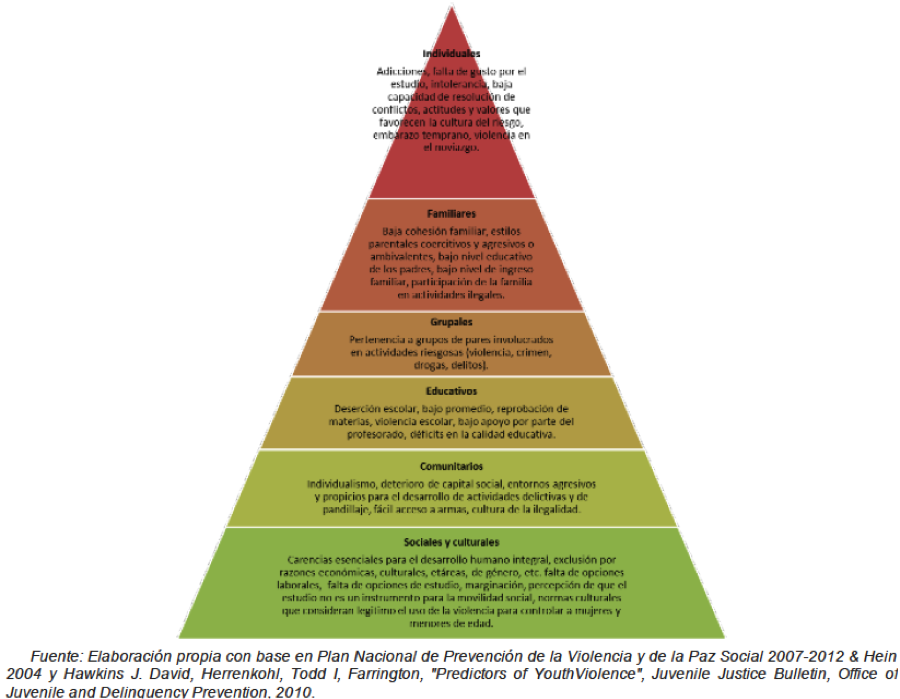
\includegraphics{img/piramide.png}

\end{frame}

\begin{frame}{Factores de Riesgo}

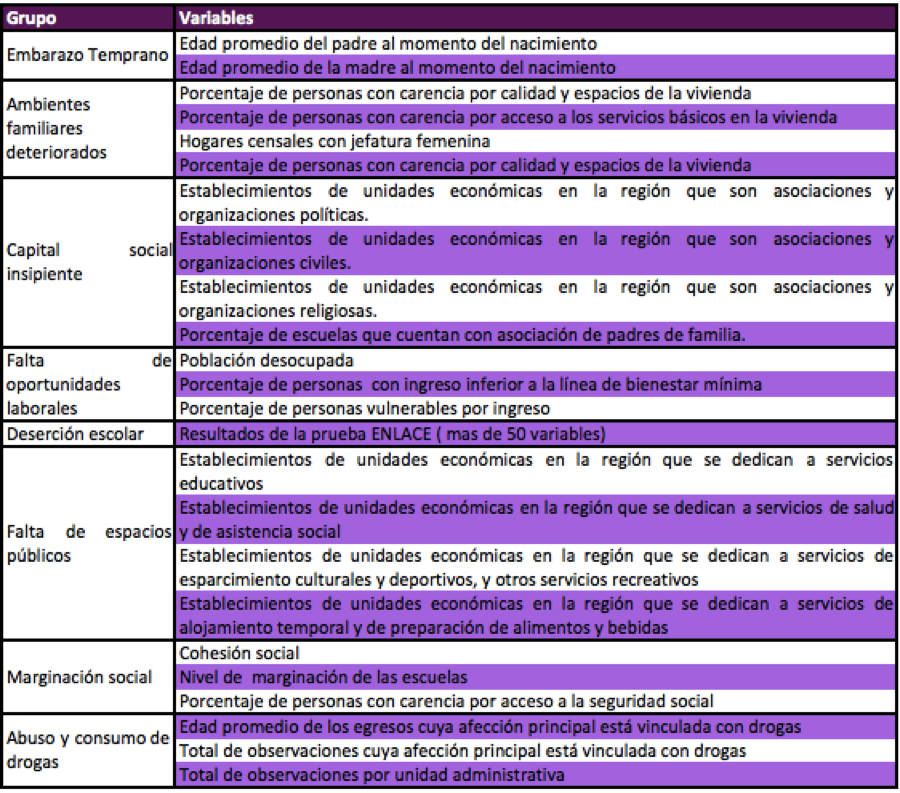
\includegraphics{img/factores_riesgo.png}

\end{frame}

\begin{frame}{Objetivo}

-El objetivo de este estudio es caracterizar los municipios del país
entorno a los diferentes factores de riesgo que el programa busca
atender. Además, se busca generar recomendaciones para identificar las
buenas prácticas y poder hacer una gestión más eficiente de los recursos
del presupuesto federal

\end{frame}

\begin{frame}{Consulta con Expertos}

\begin{itemize}
\itemsep1pt\parskip0pt\parsep0pt
\item
  México Evalúa
\item
  COLMEX Dr.Arturo Alvarado
\item
  CIDE, Dr.~Carlos Vilalta
\end{itemize}

\end{frame}

\begin{frame}{Fuentes de datos}

\begin{itemize}
\itemsep1pt\parskip0pt\parsep0pt
\item
  CONEVAL: Resago social (censo 2010).
\item
  INEGI:

  \begin{itemize}
  \itemsep1pt\parskip0pt\parsep0pt
  \item
    Censo
  \item
    Encuesta Nacional sobre la Dinaámica de las Relaciones de los
    Hogares (ENDIREH)
  \item
    Encuesta Nacional de Victimización y Percepción sobre Seguridad
    Pública (ENVIPE)
  \item
    Directorio Estadístico Nacional de Unidades Económicas (DENUE)
  \end{itemize}
\item
  SEP

  \begin{itemize}
  \itemsep1pt\parskip0pt\parsep0pt
  \item
    Censo educativo (2013).
  \item
    ENLACE (2013).
  \end{itemize}
\item
  Encuesta Nacional de Cultura Política y Prácticas Ciudadanas (ENCUP,
  Gob e INEGI).
\item
  Sistema Nacional de Información de Salud (SINAIS)

  \begin{itemize}
  \itemsep1pt\parskip0pt\parsep0pt
  \item
    Egresos hospitalarios
  \item
    Recursos de salud
  \end{itemize}
\item
  Secretariado Ejecutivo Sistema Nacional de Seguridad Pública (SESNSP,
  Variable dependiente).
\end{itemize}

\end{frame}

\begin{frame}{Problemas con los datos y modelado.}

\begin{itemize}
\itemsep1pt\parskip0pt\parsep0pt
\item
  Años.

  \begin{itemize}
  \itemsep1pt\parskip0pt\parsep0pt
  \item
    De cada fuente de los datos se toma el último año.
  \end{itemize}
\item
  Medición de los factores de riesgo.
\item
  Encuestas

  \begin{itemize}
  \itemsep1pt\parskip0pt\parsep0pt
  \item
    Son estatales.
  \item
    A todos los municipios.
  \item
    Considerar el muestreso de los municipios (No es trivial).
  \end{itemize}
\item
  Espacios públicos.
\item
  NA's.

  \begin{itemize}
  \itemsep1pt\parskip0pt\parsep0pt
  \item
    Registros admin: 0's.
  \item
    Encuestas: muestreo en todos los mun.
  \end{itemize}
\item
  Enlace:

  \begin{itemize}
  \itemsep1pt\parskip0pt\parsep0pt
  \item
    Hay menos registros públicos que los se reportan.
  \end{itemize}
\end{itemize}

\end{frame}

\begin{frame}{Correcciones}

\begin{itemize}
\itemsep1pt\parskip0pt\parsep0pt
\item
  Dadas las recomendaciones de la presentación del anteproyecto se tomo
  solamente aquellos municipios con poblaciones mayores a los 40 mil
  habitantes
\item
  A los registros administrativos censales se les imputo ceros
\item
  Se ajustaron las variables por densidad poblacional
\end{itemize}

\end{frame}

\begin{frame}{Correcciones}

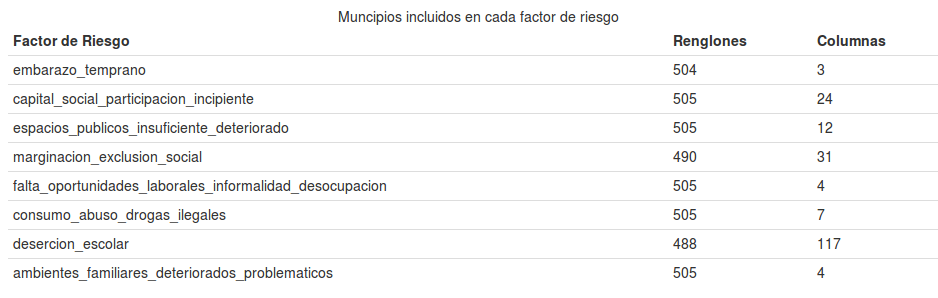
\includegraphics{img/municipios_incluidos.png}

\end{frame}

\section{Estadística Descriptiva
Inicial}\label{estadistica-descriptiva-inicial}

\begin{frame}{Embarazo temprano}

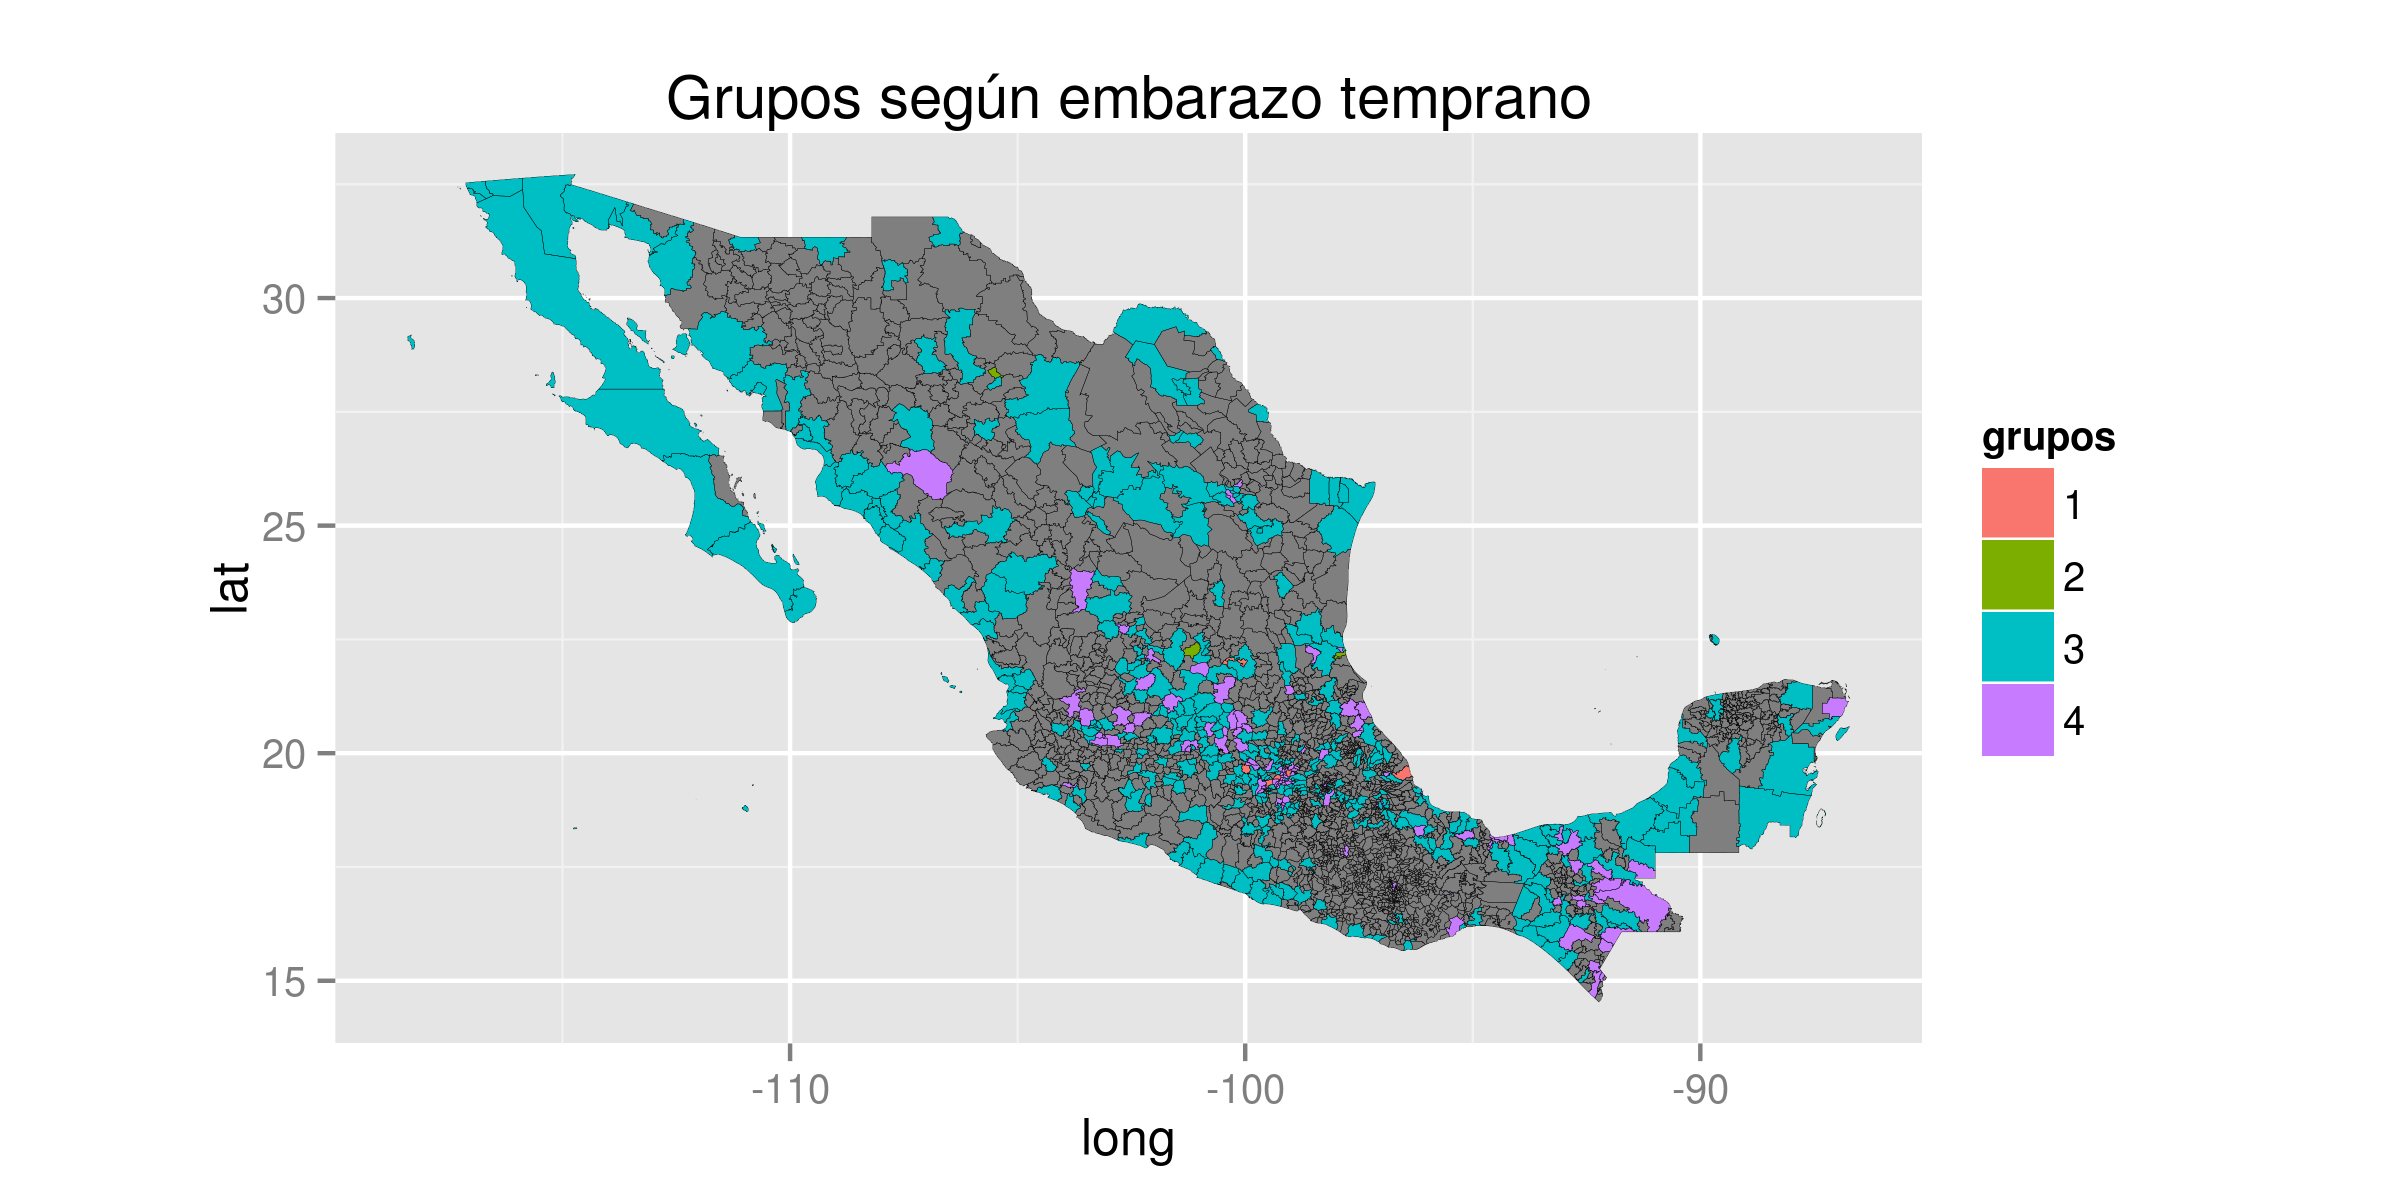
\includegraphics{img/mapa_embarazo_temprano.png}

\end{frame}

\begin{frame}{Marginación y exclusión social}

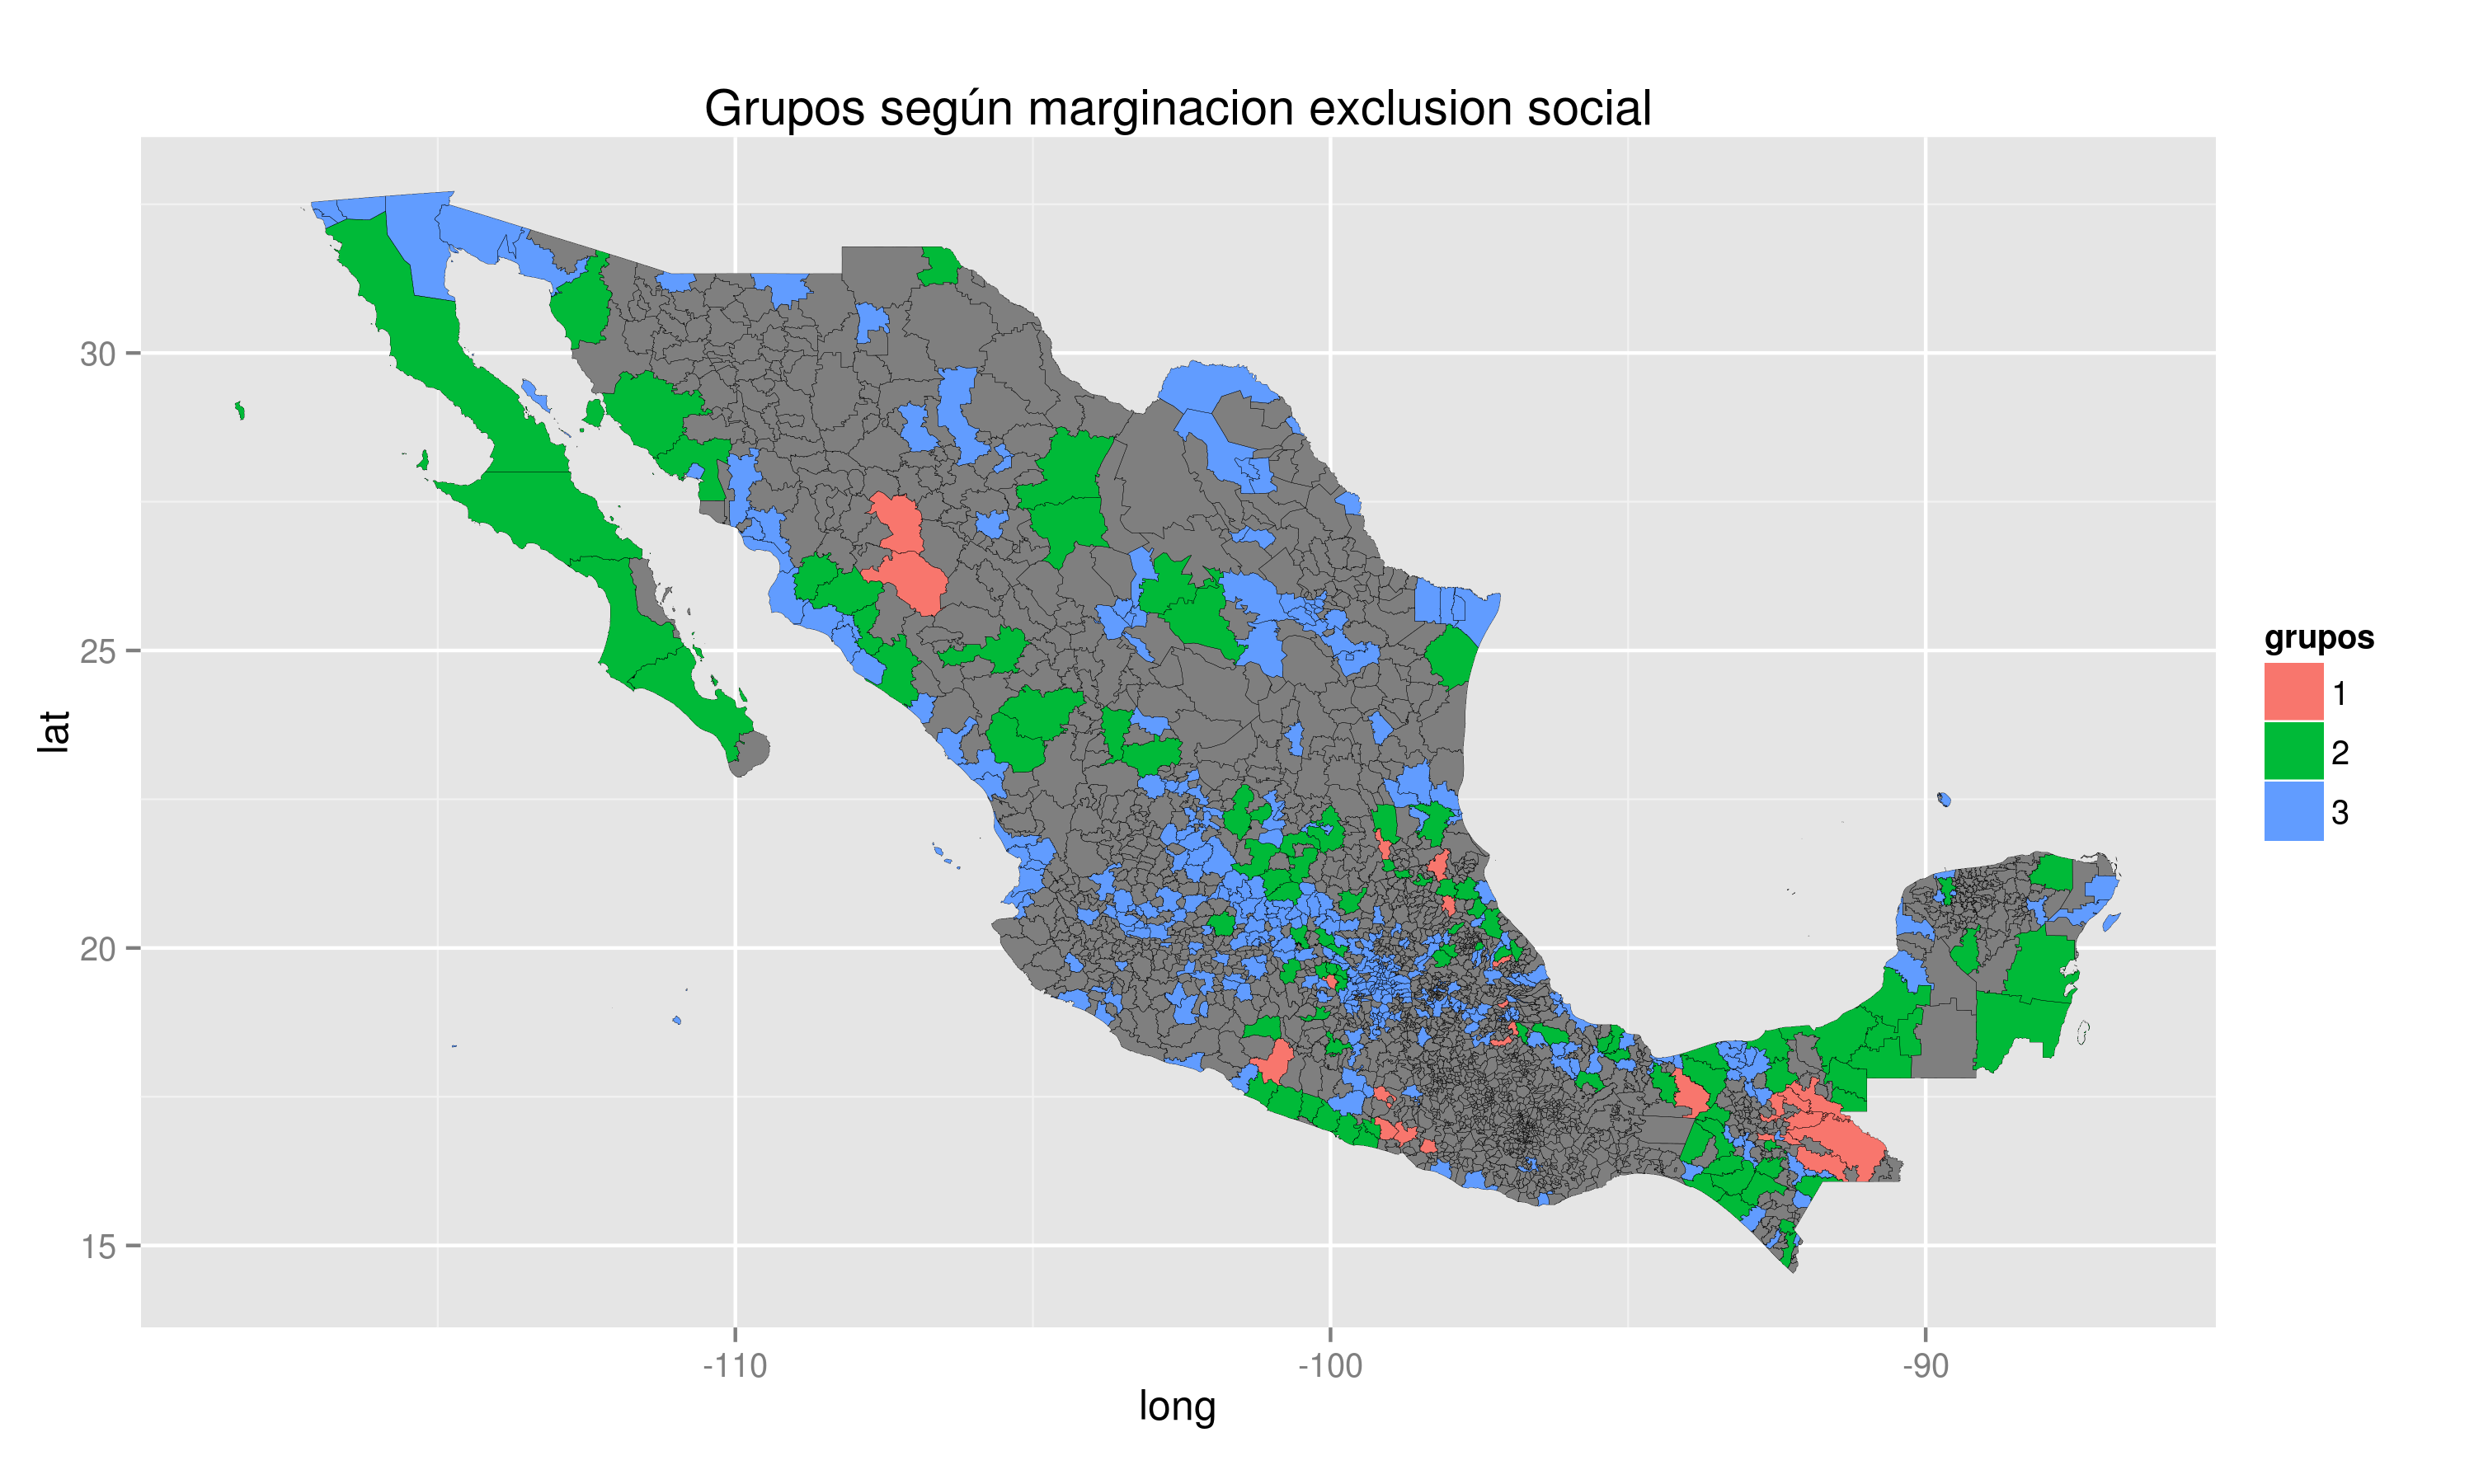
\includegraphics{img/mapa_marginacion_exclusion_social.png}

\end{frame}

\begin{frame}{Falta de oportunidades laborales, informalidad y
desocupación}

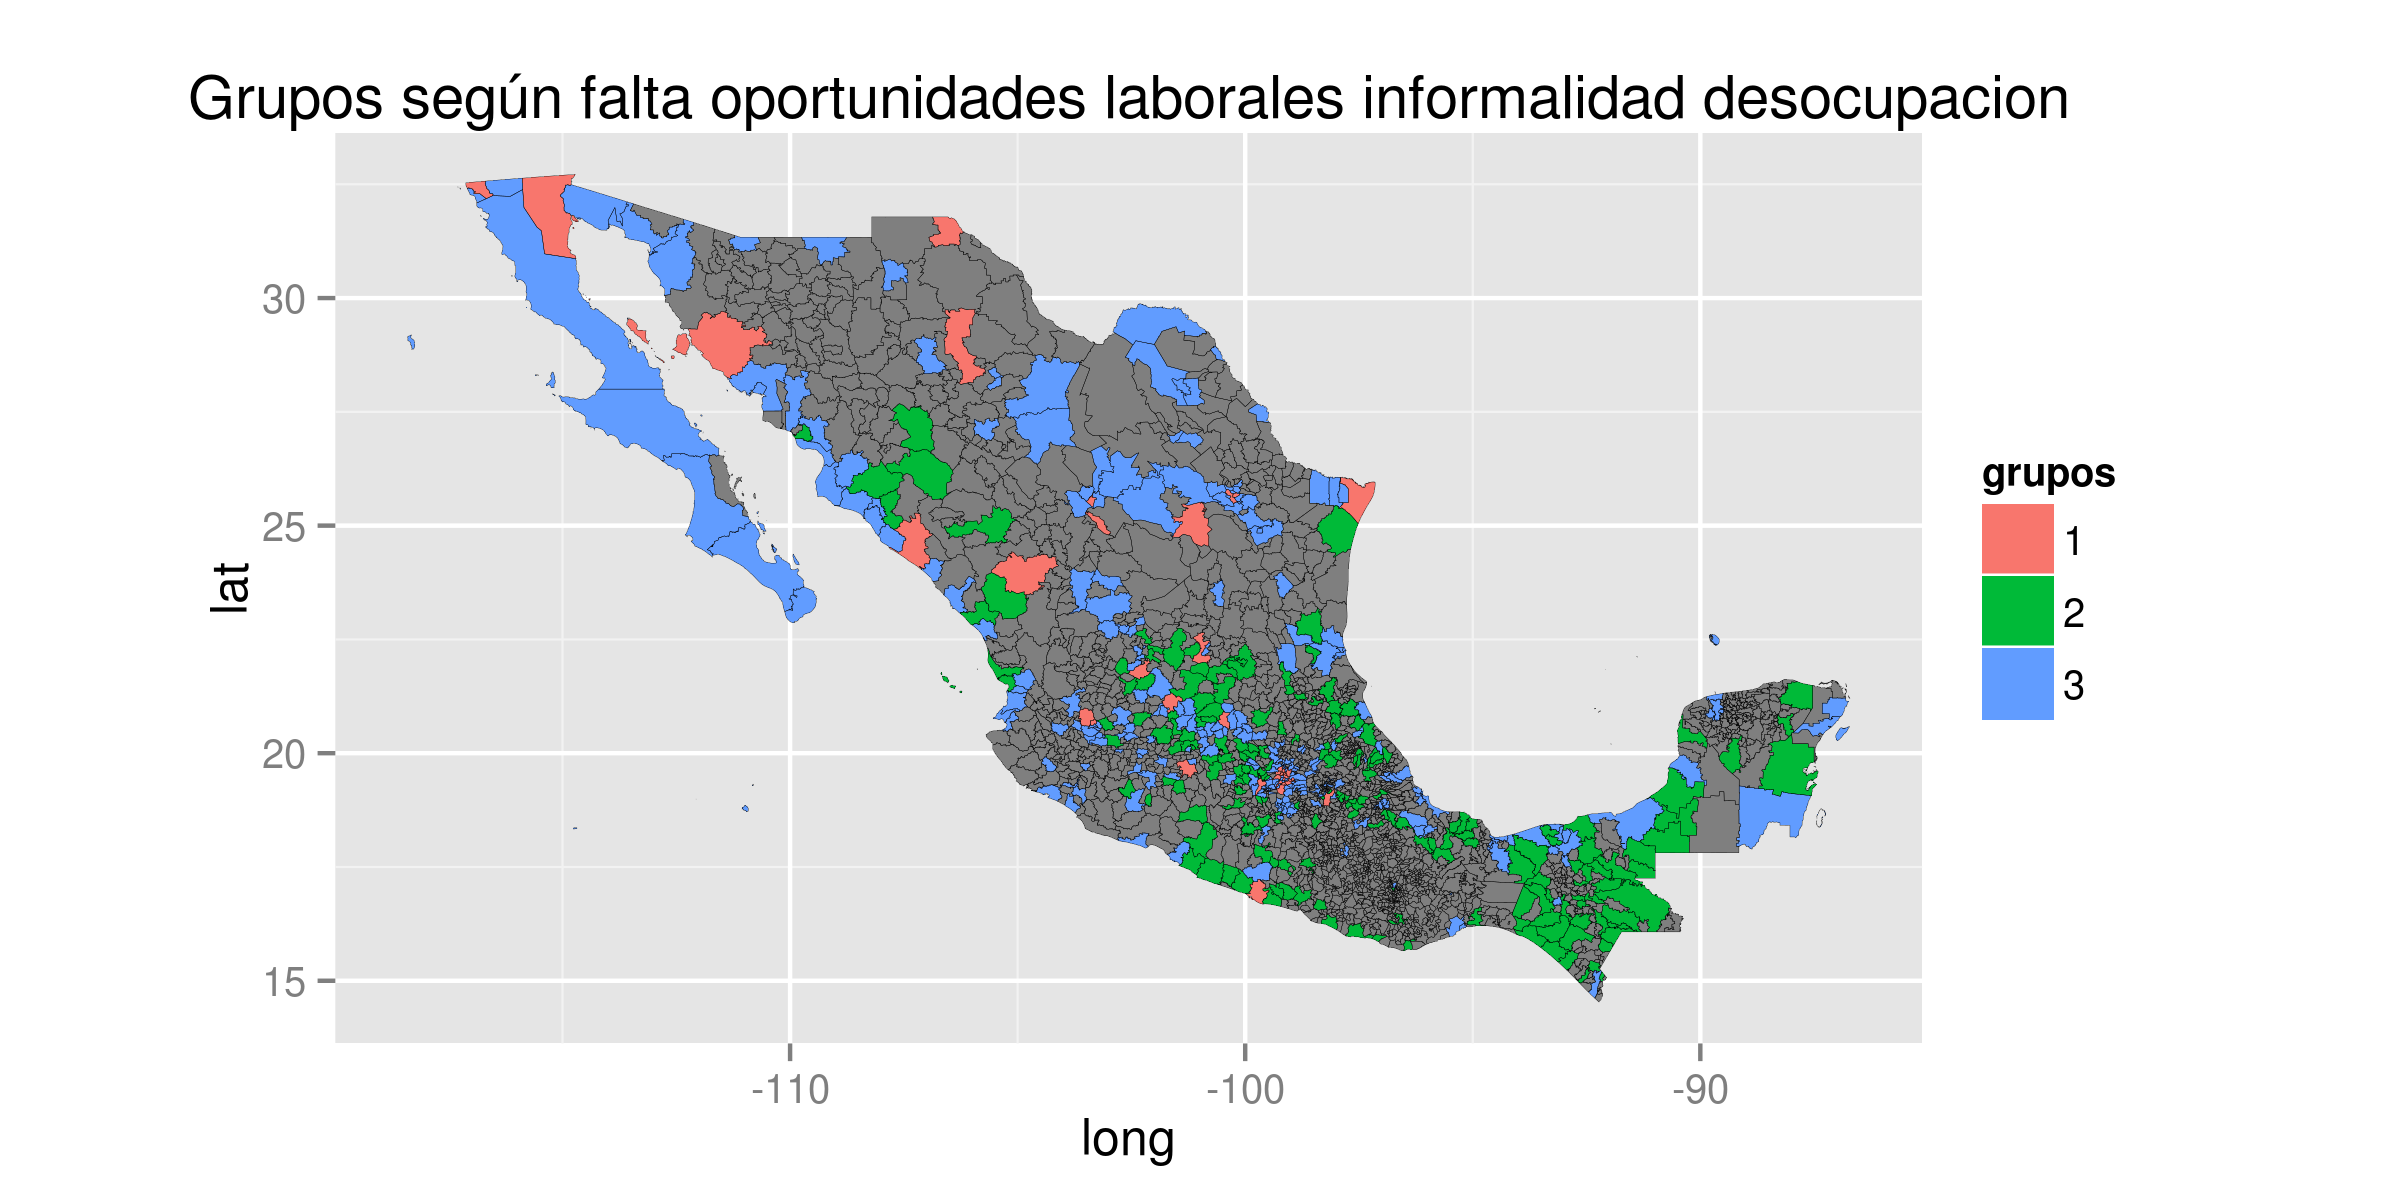
\includegraphics{img/mapa_falta_oportunidades_laborales_informalidad_desocupacion.png}

\end{frame}

\begin{frame}{Espacios públicos insuficientes y deteriorados}

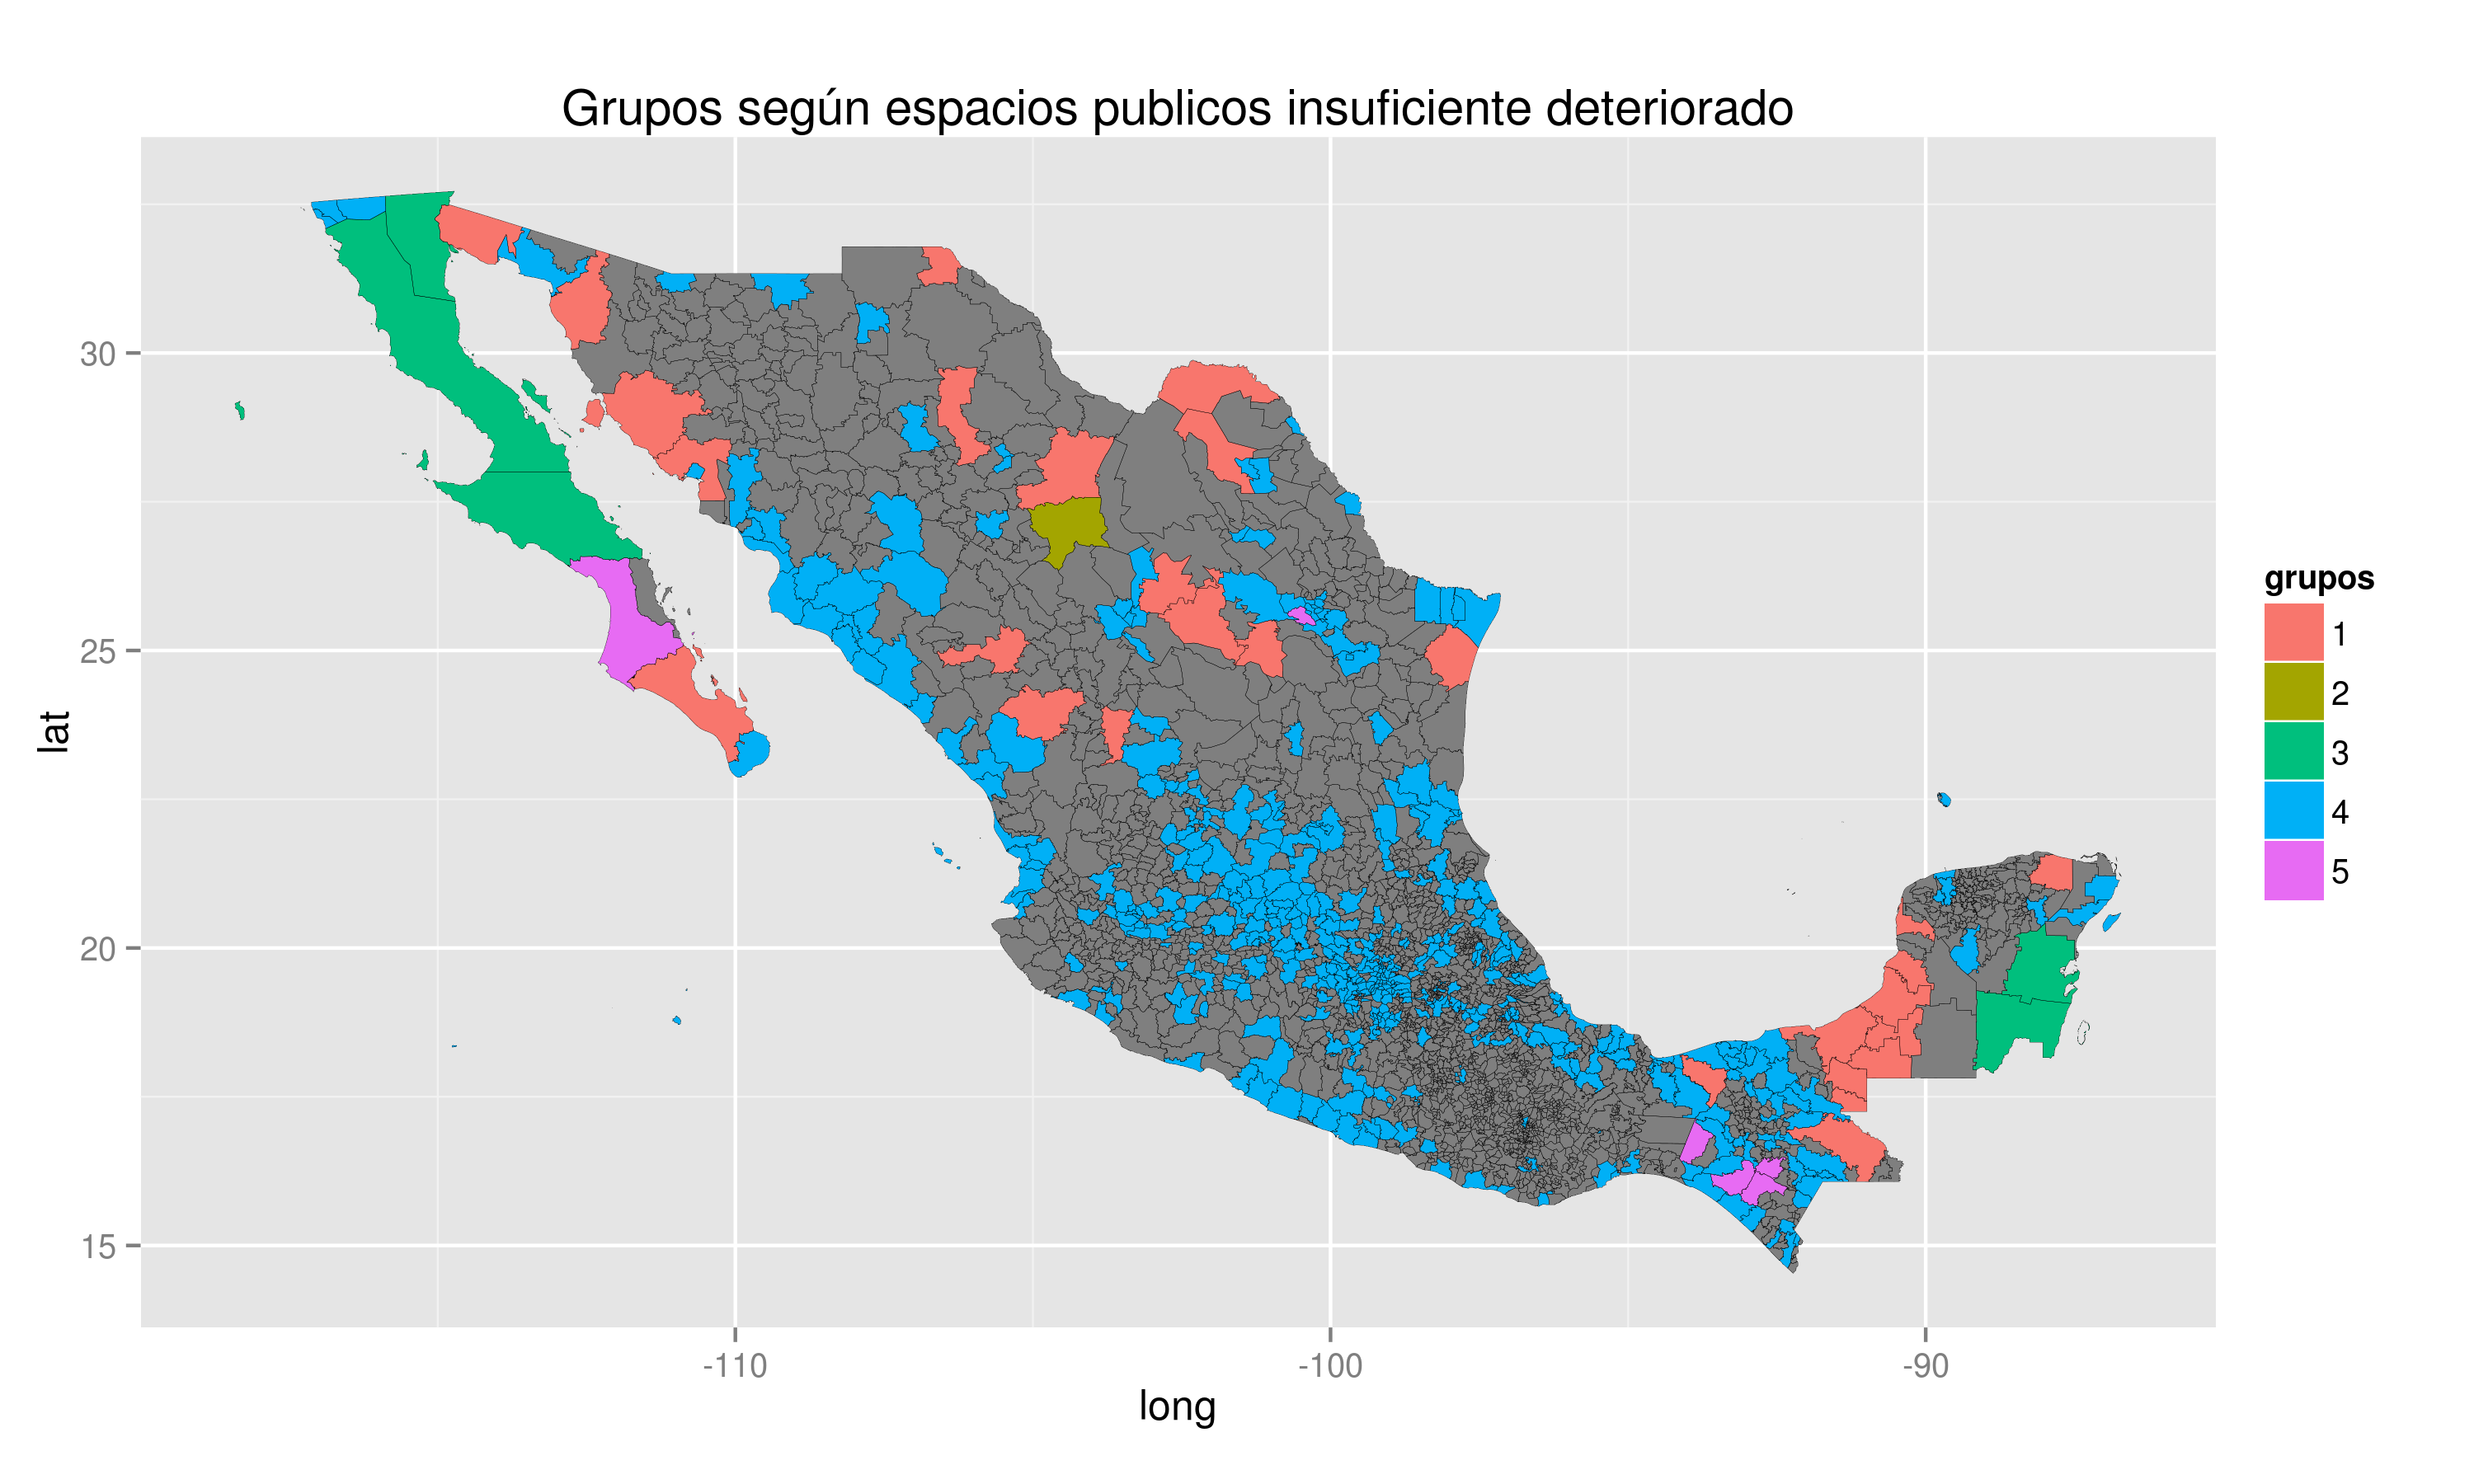
\includegraphics{img/mapa_espacios_publicos_insuficiente_deteriorado.png}

\end{frame}

\begin{frame}{Capital social y participación incipiente}

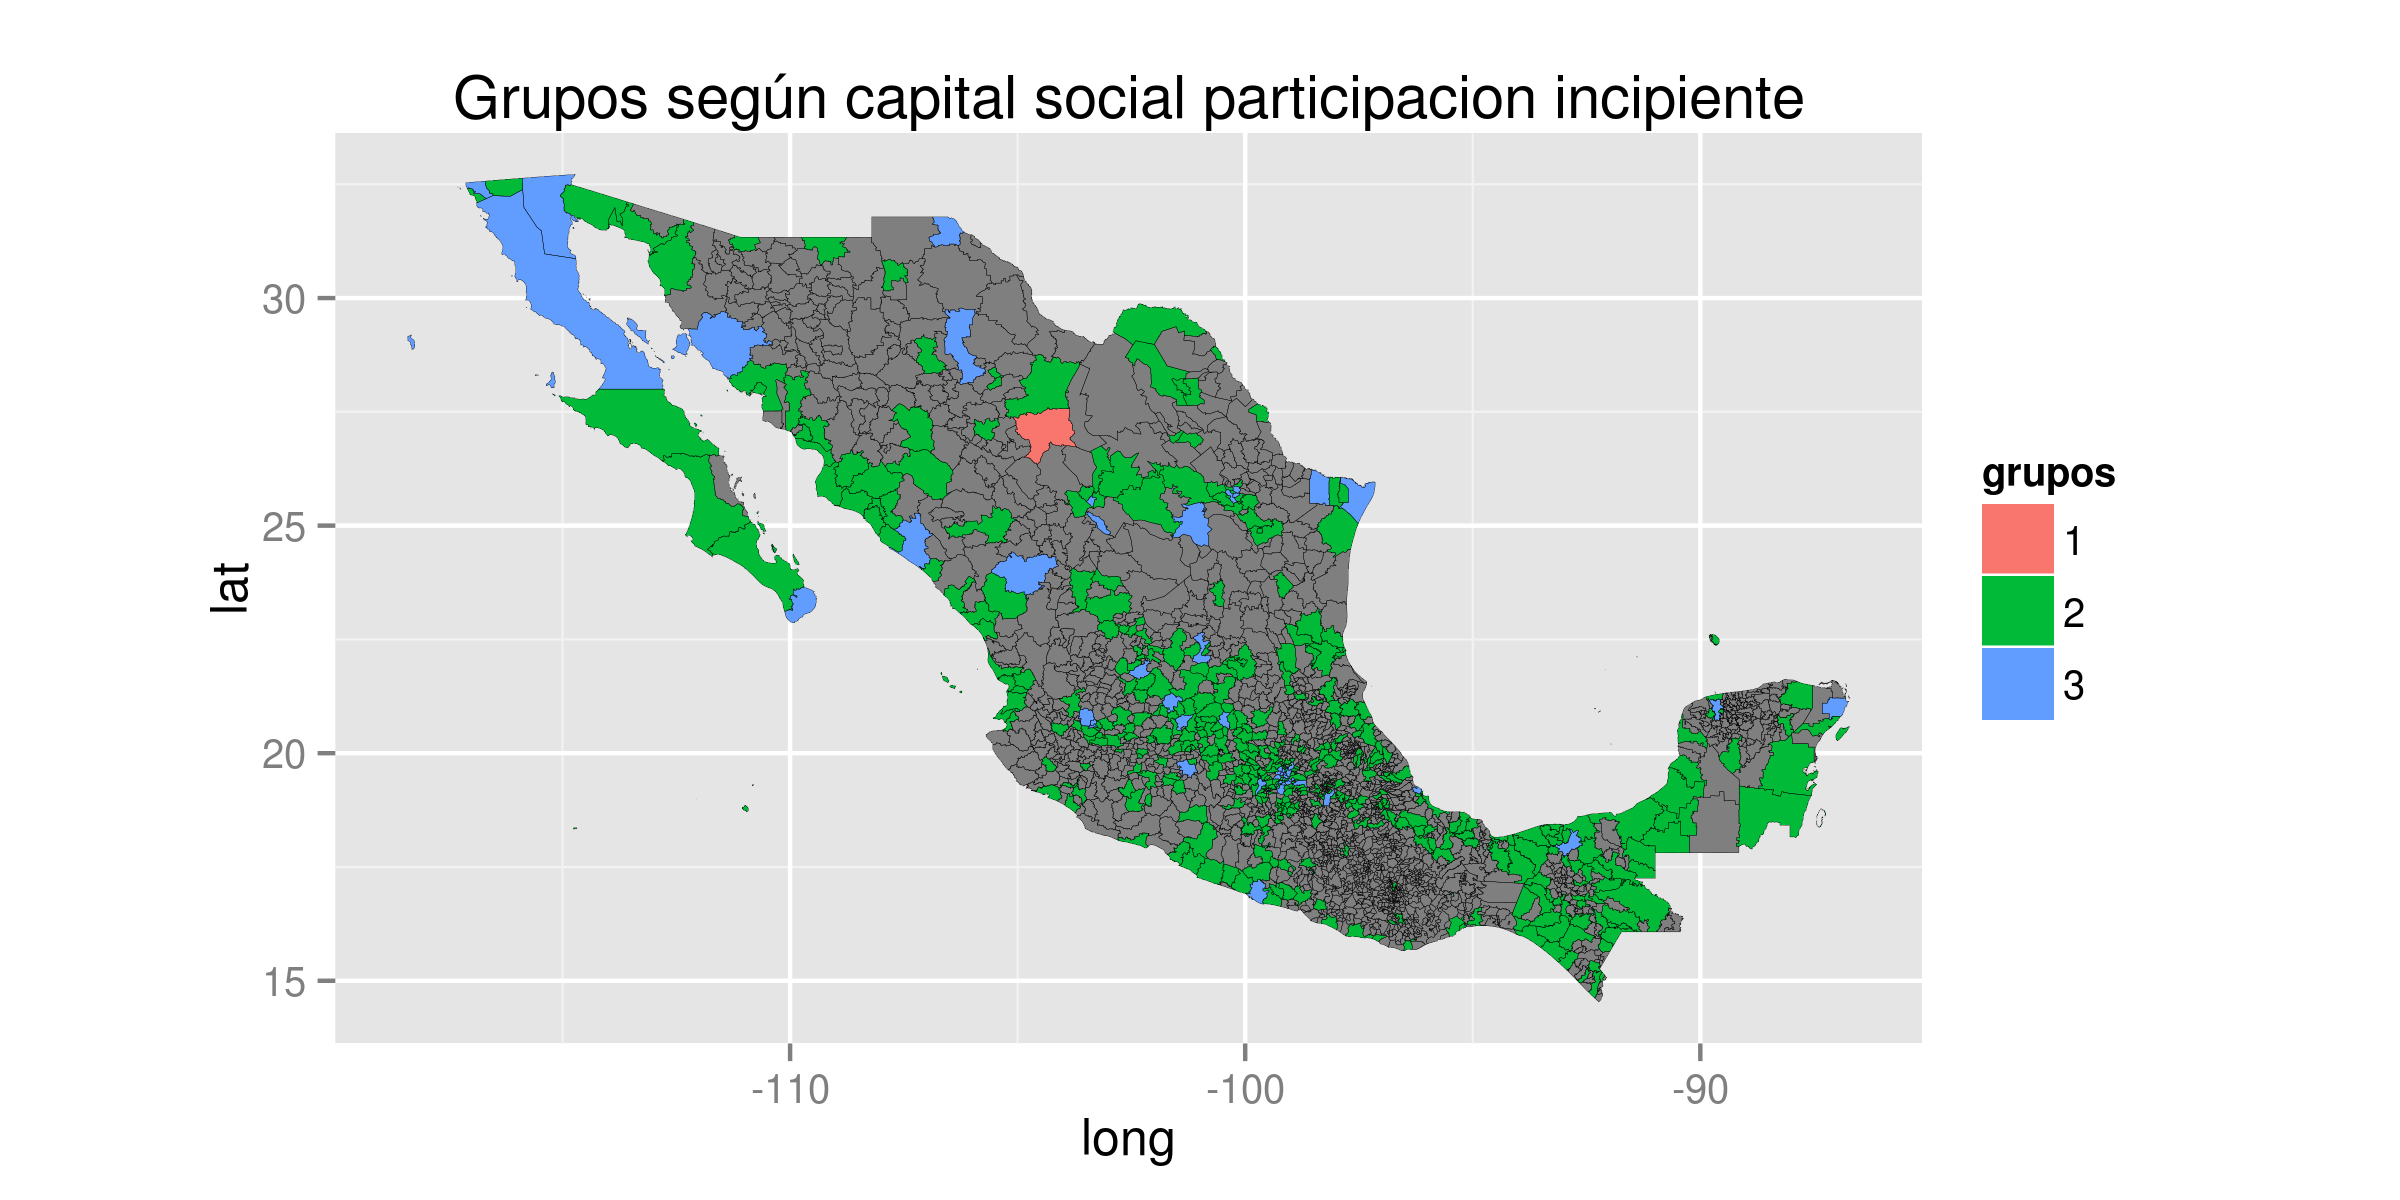
\includegraphics{img/mapa_capital_social_participacion_incipiente.png}

\end{frame}

\begin{frame}{Deserción escolar}

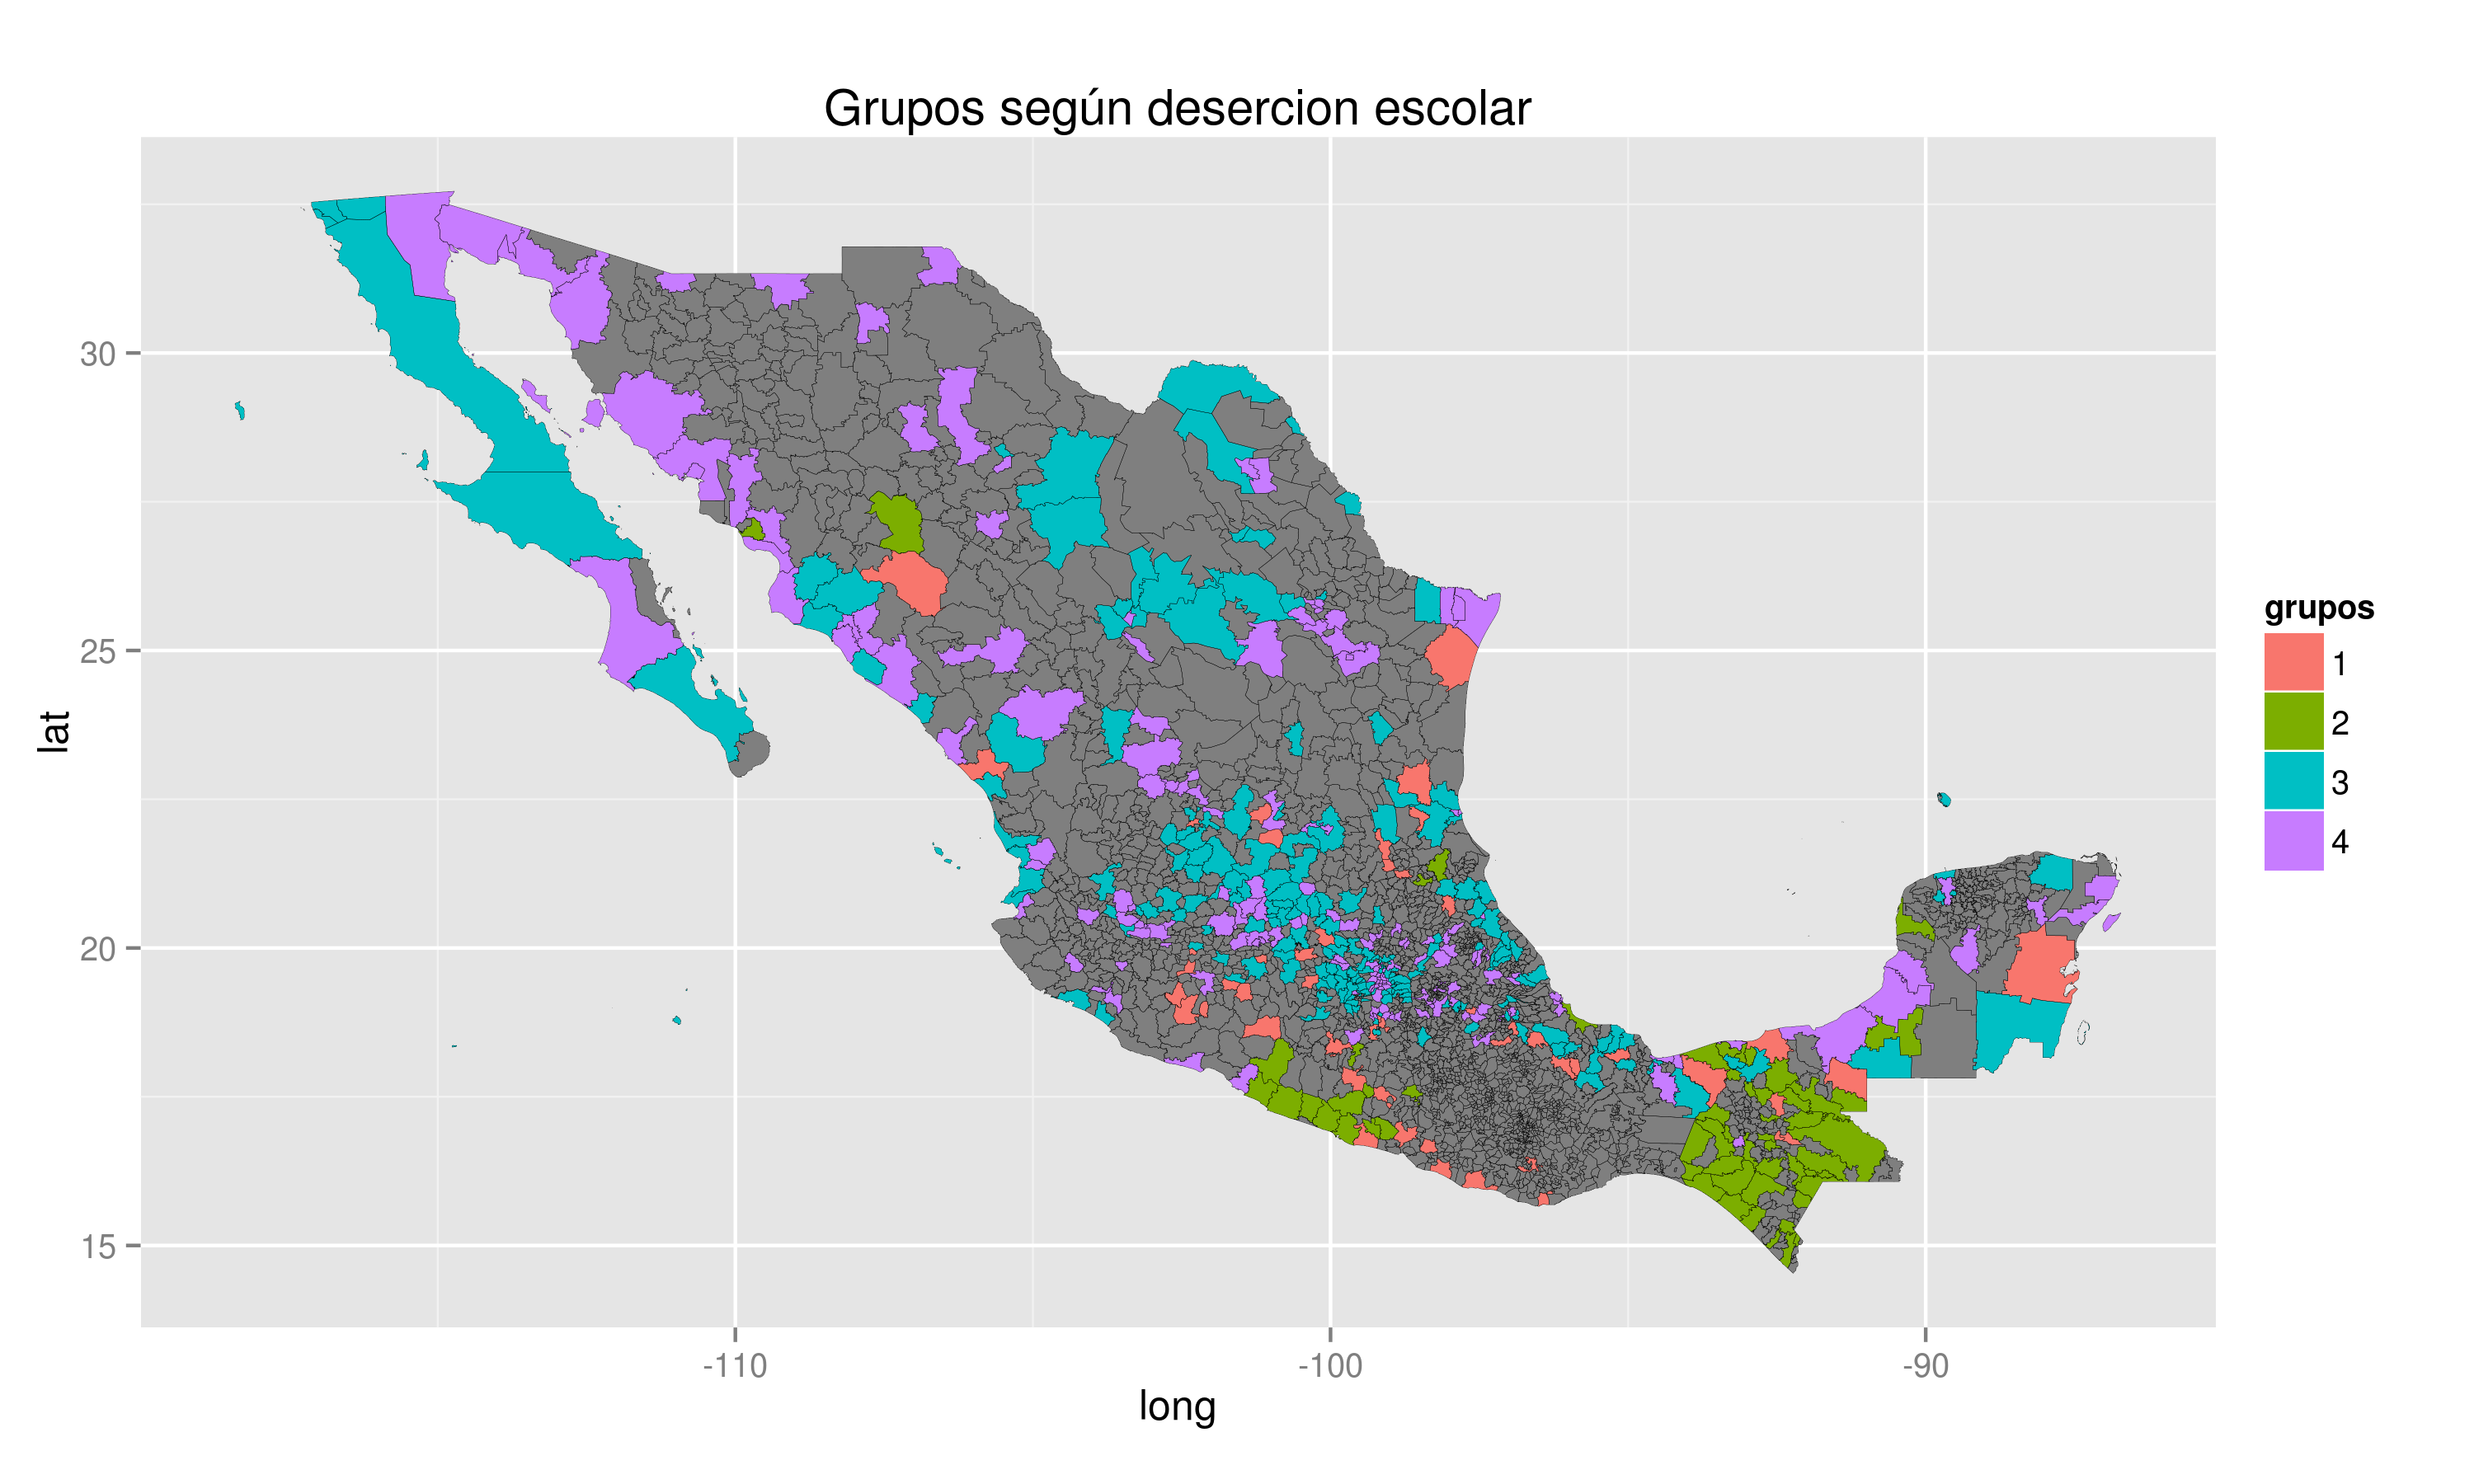
\includegraphics{img/mapa_desercion_escolar.png}

\end{frame}

\begin{frame}{Consumo y abuso de drogas legales e ilegales}

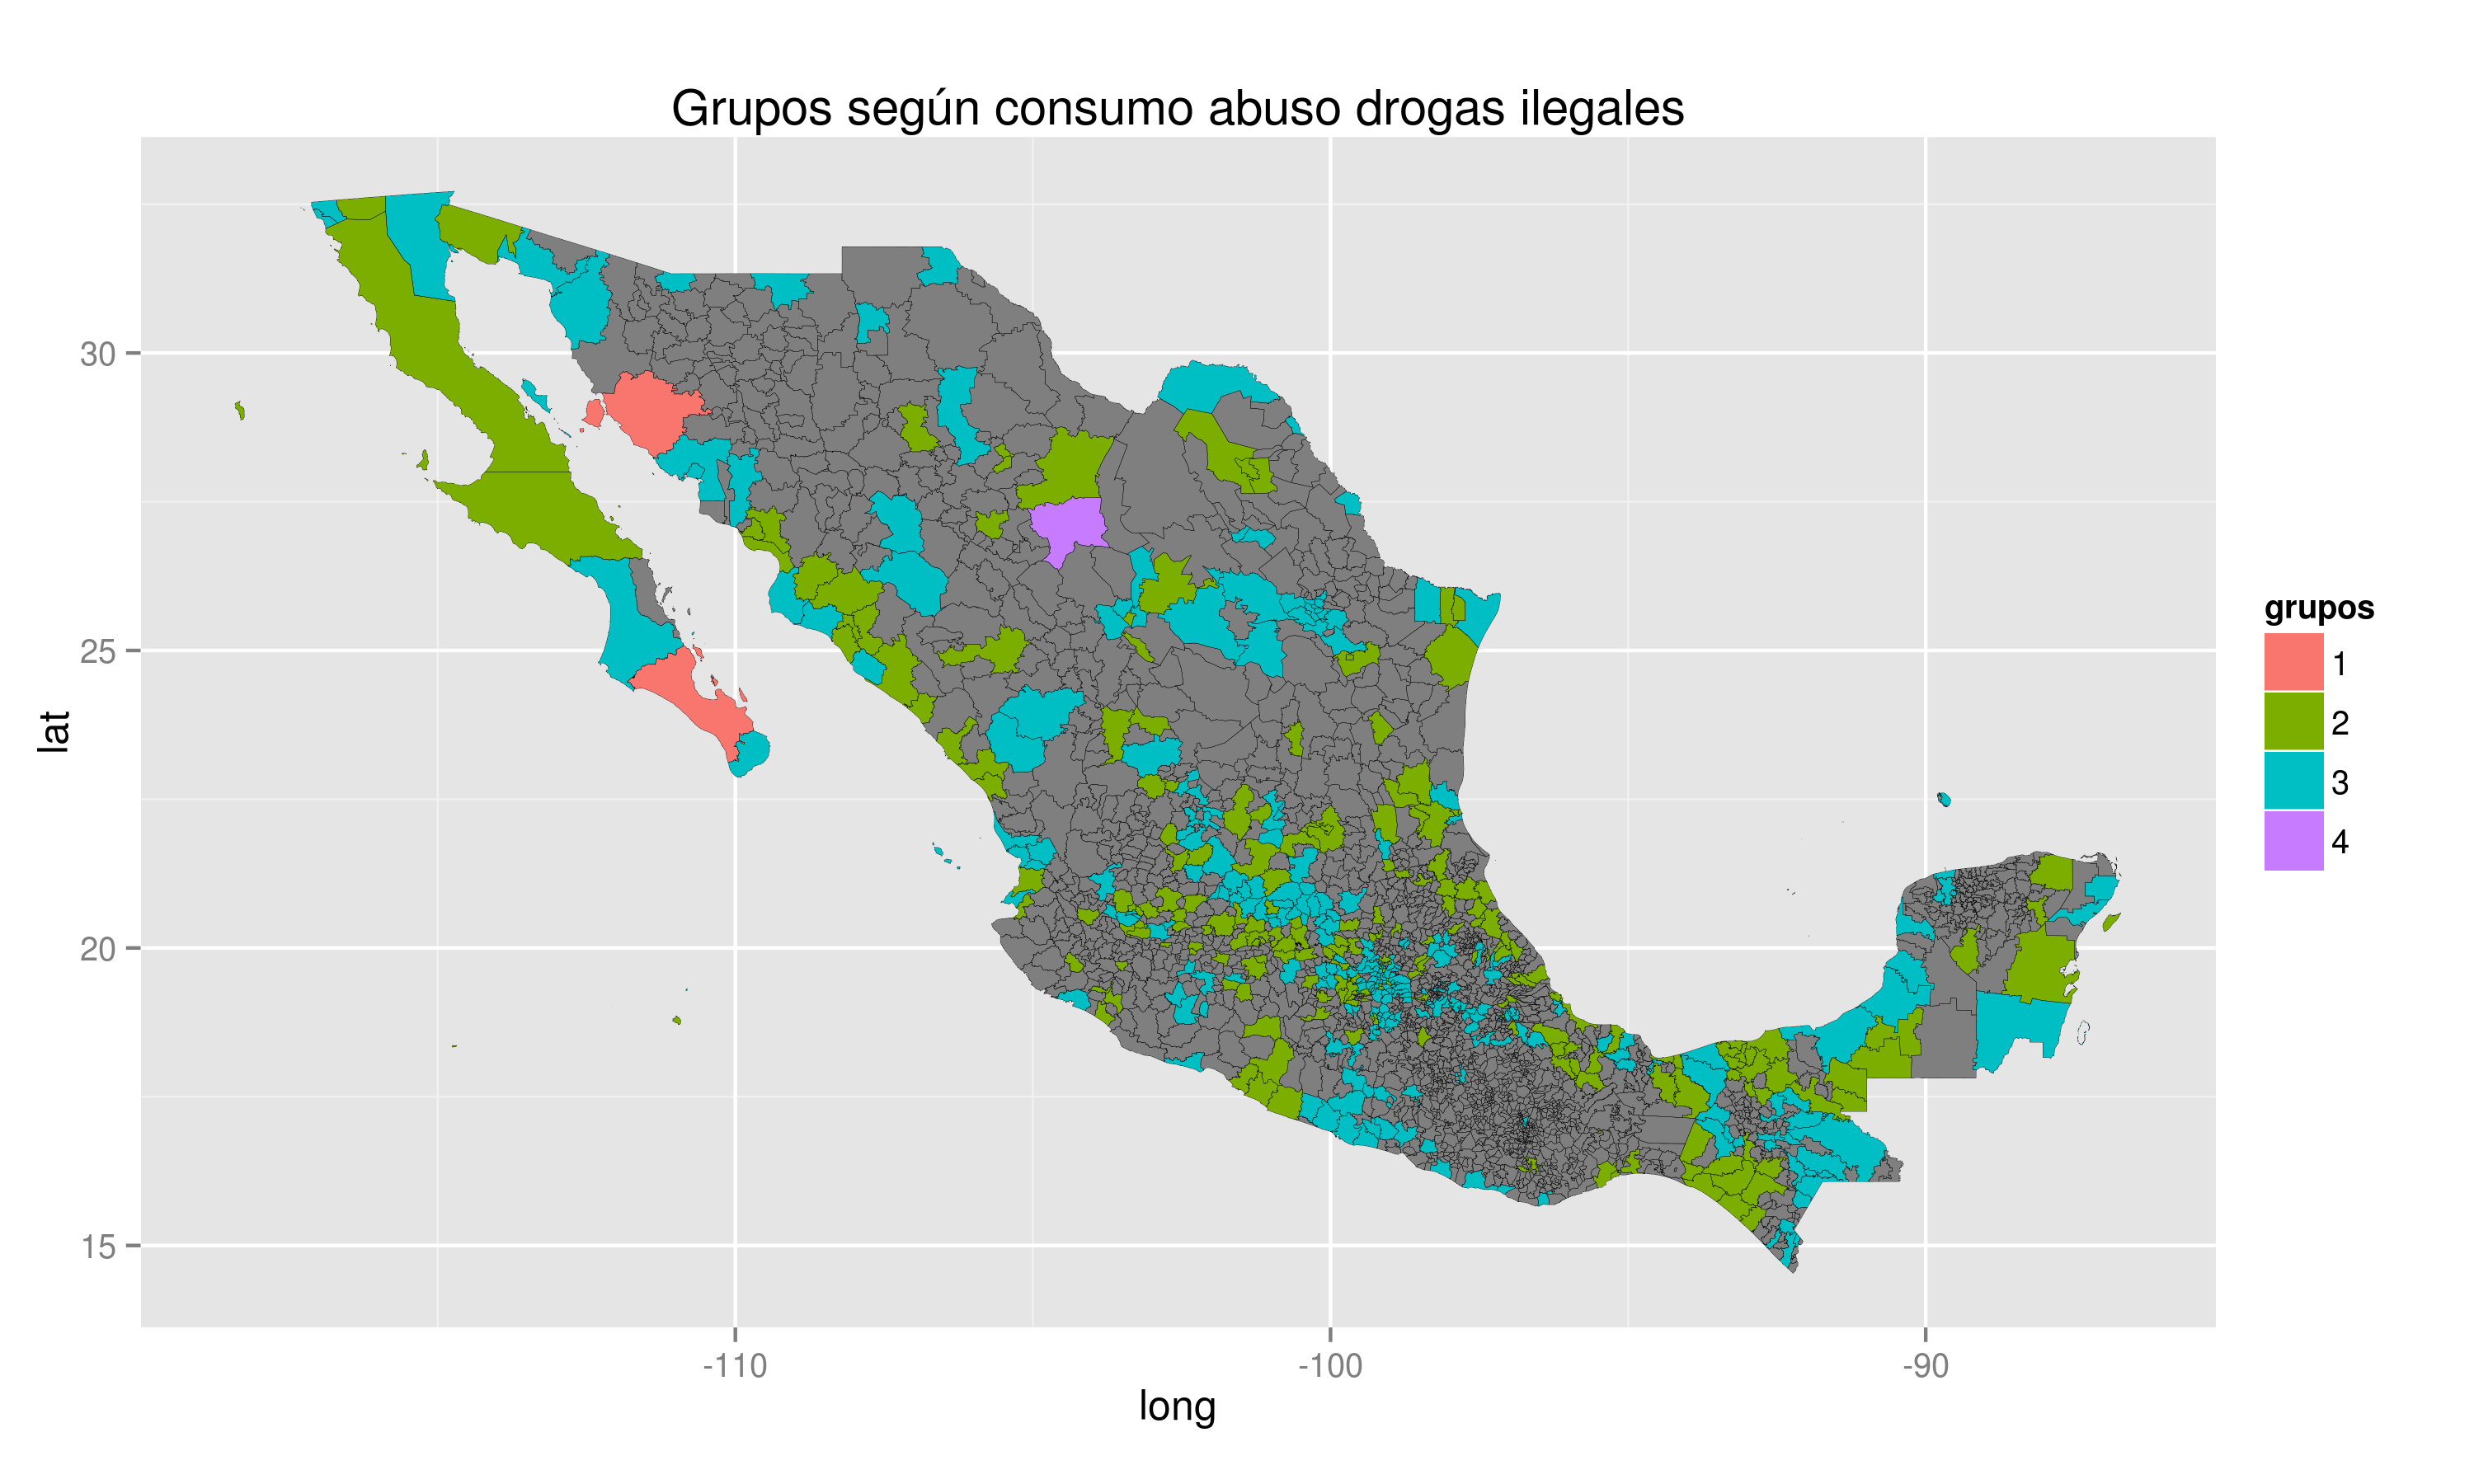
\includegraphics{img/mapa_consumo_abuso_drogas_ilegales.png}

\end{frame}

\begin{frame}{Ambientes familiares deteriorados y problemáticos}

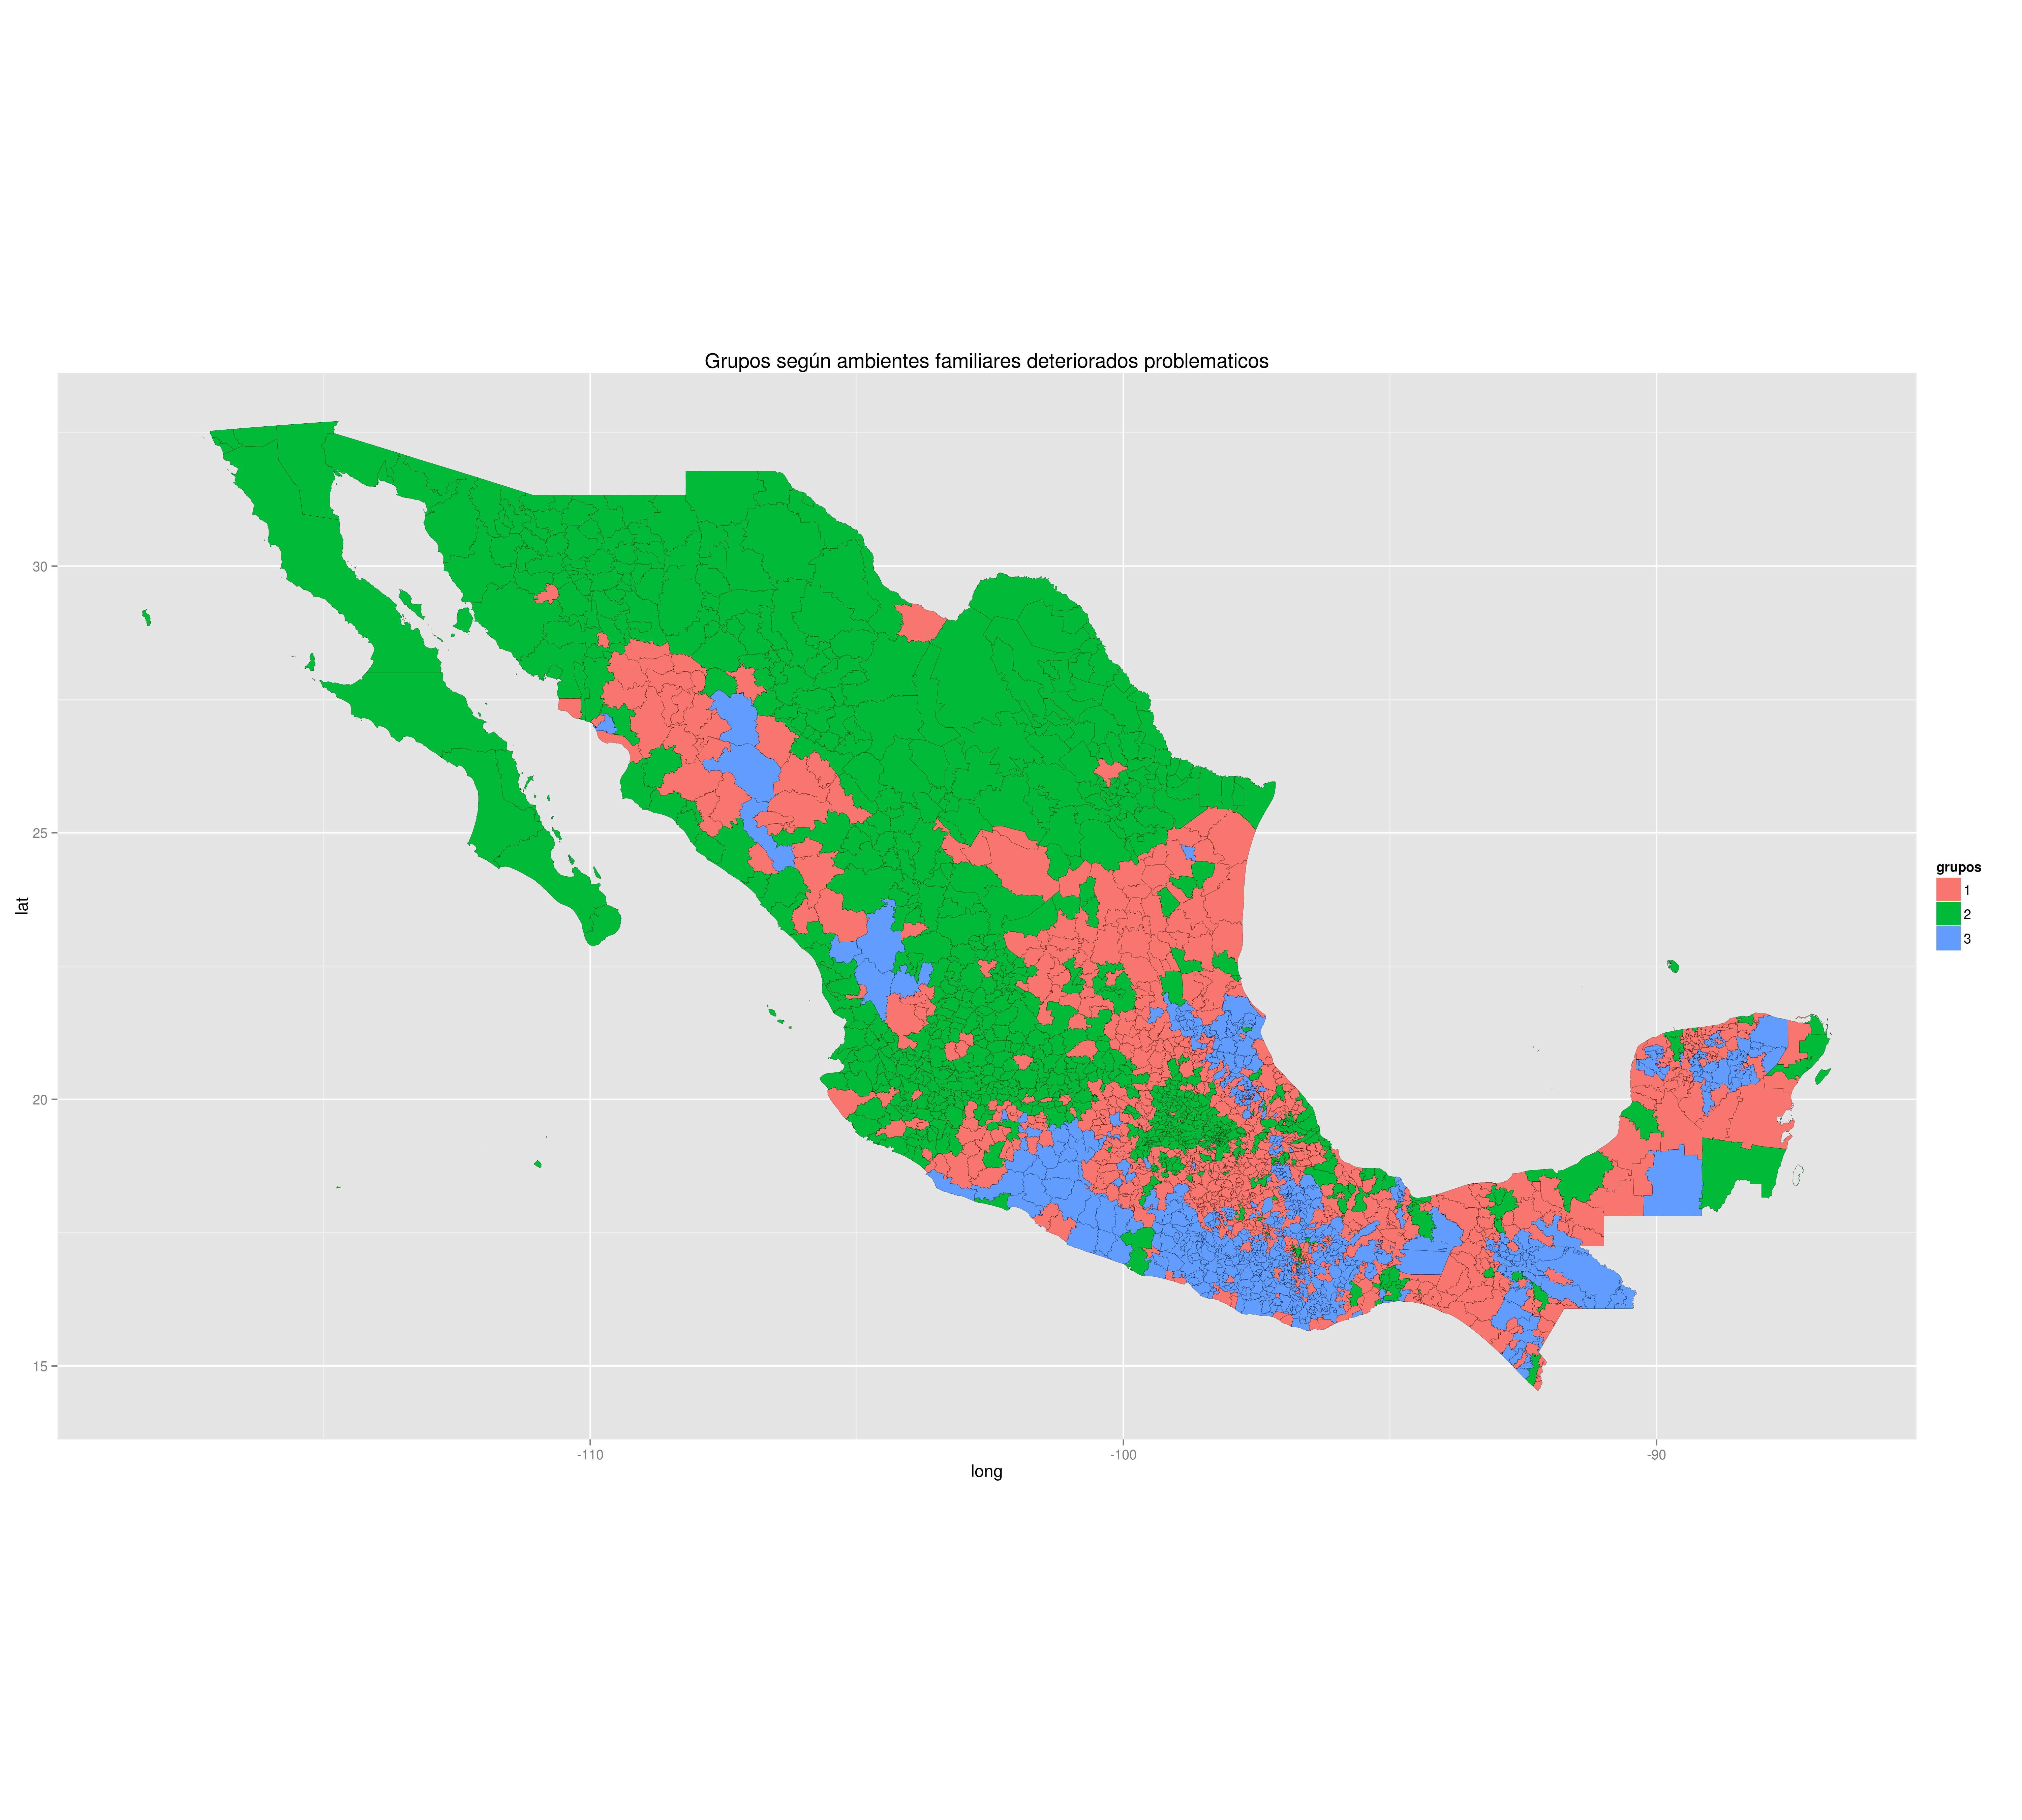
\includegraphics{img/mapa_ambientes_familiares_deteriorados_problematicos.png}

\end{frame}

\begin{frame}{Densidad dependiente}

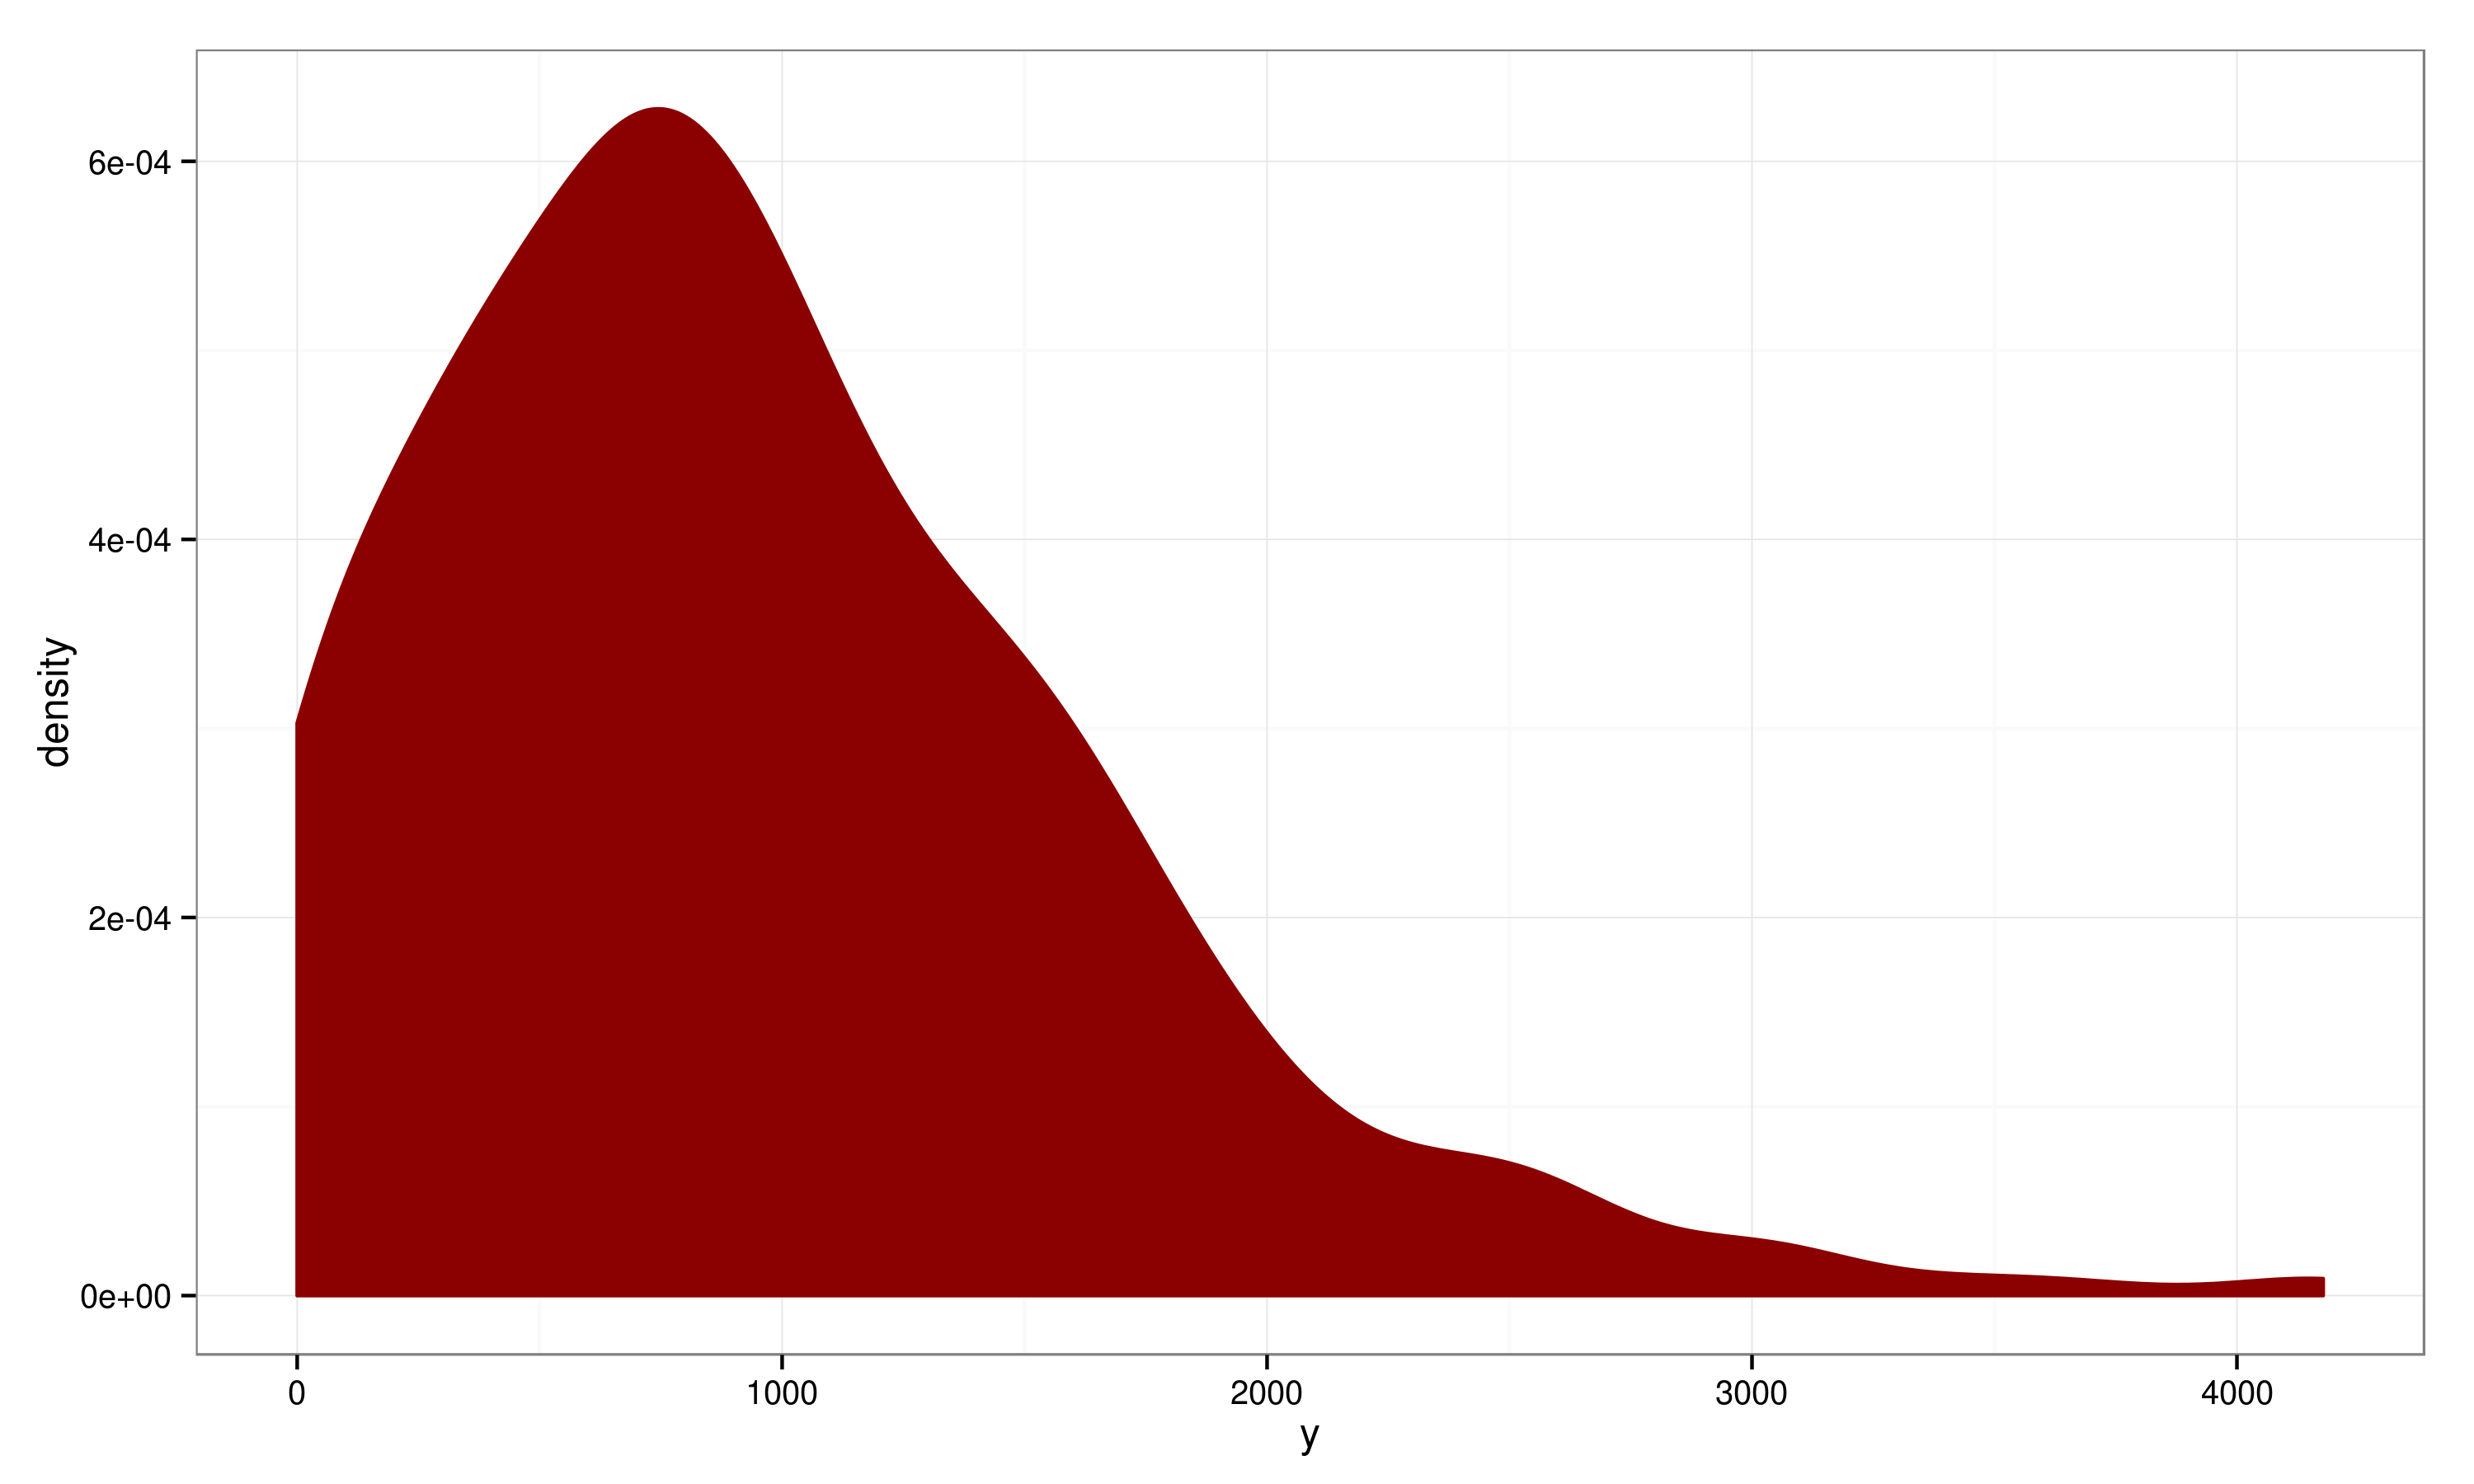
\includegraphics{img/y_log_density.png}

\end{frame}

\begin{frame}{Outliers}

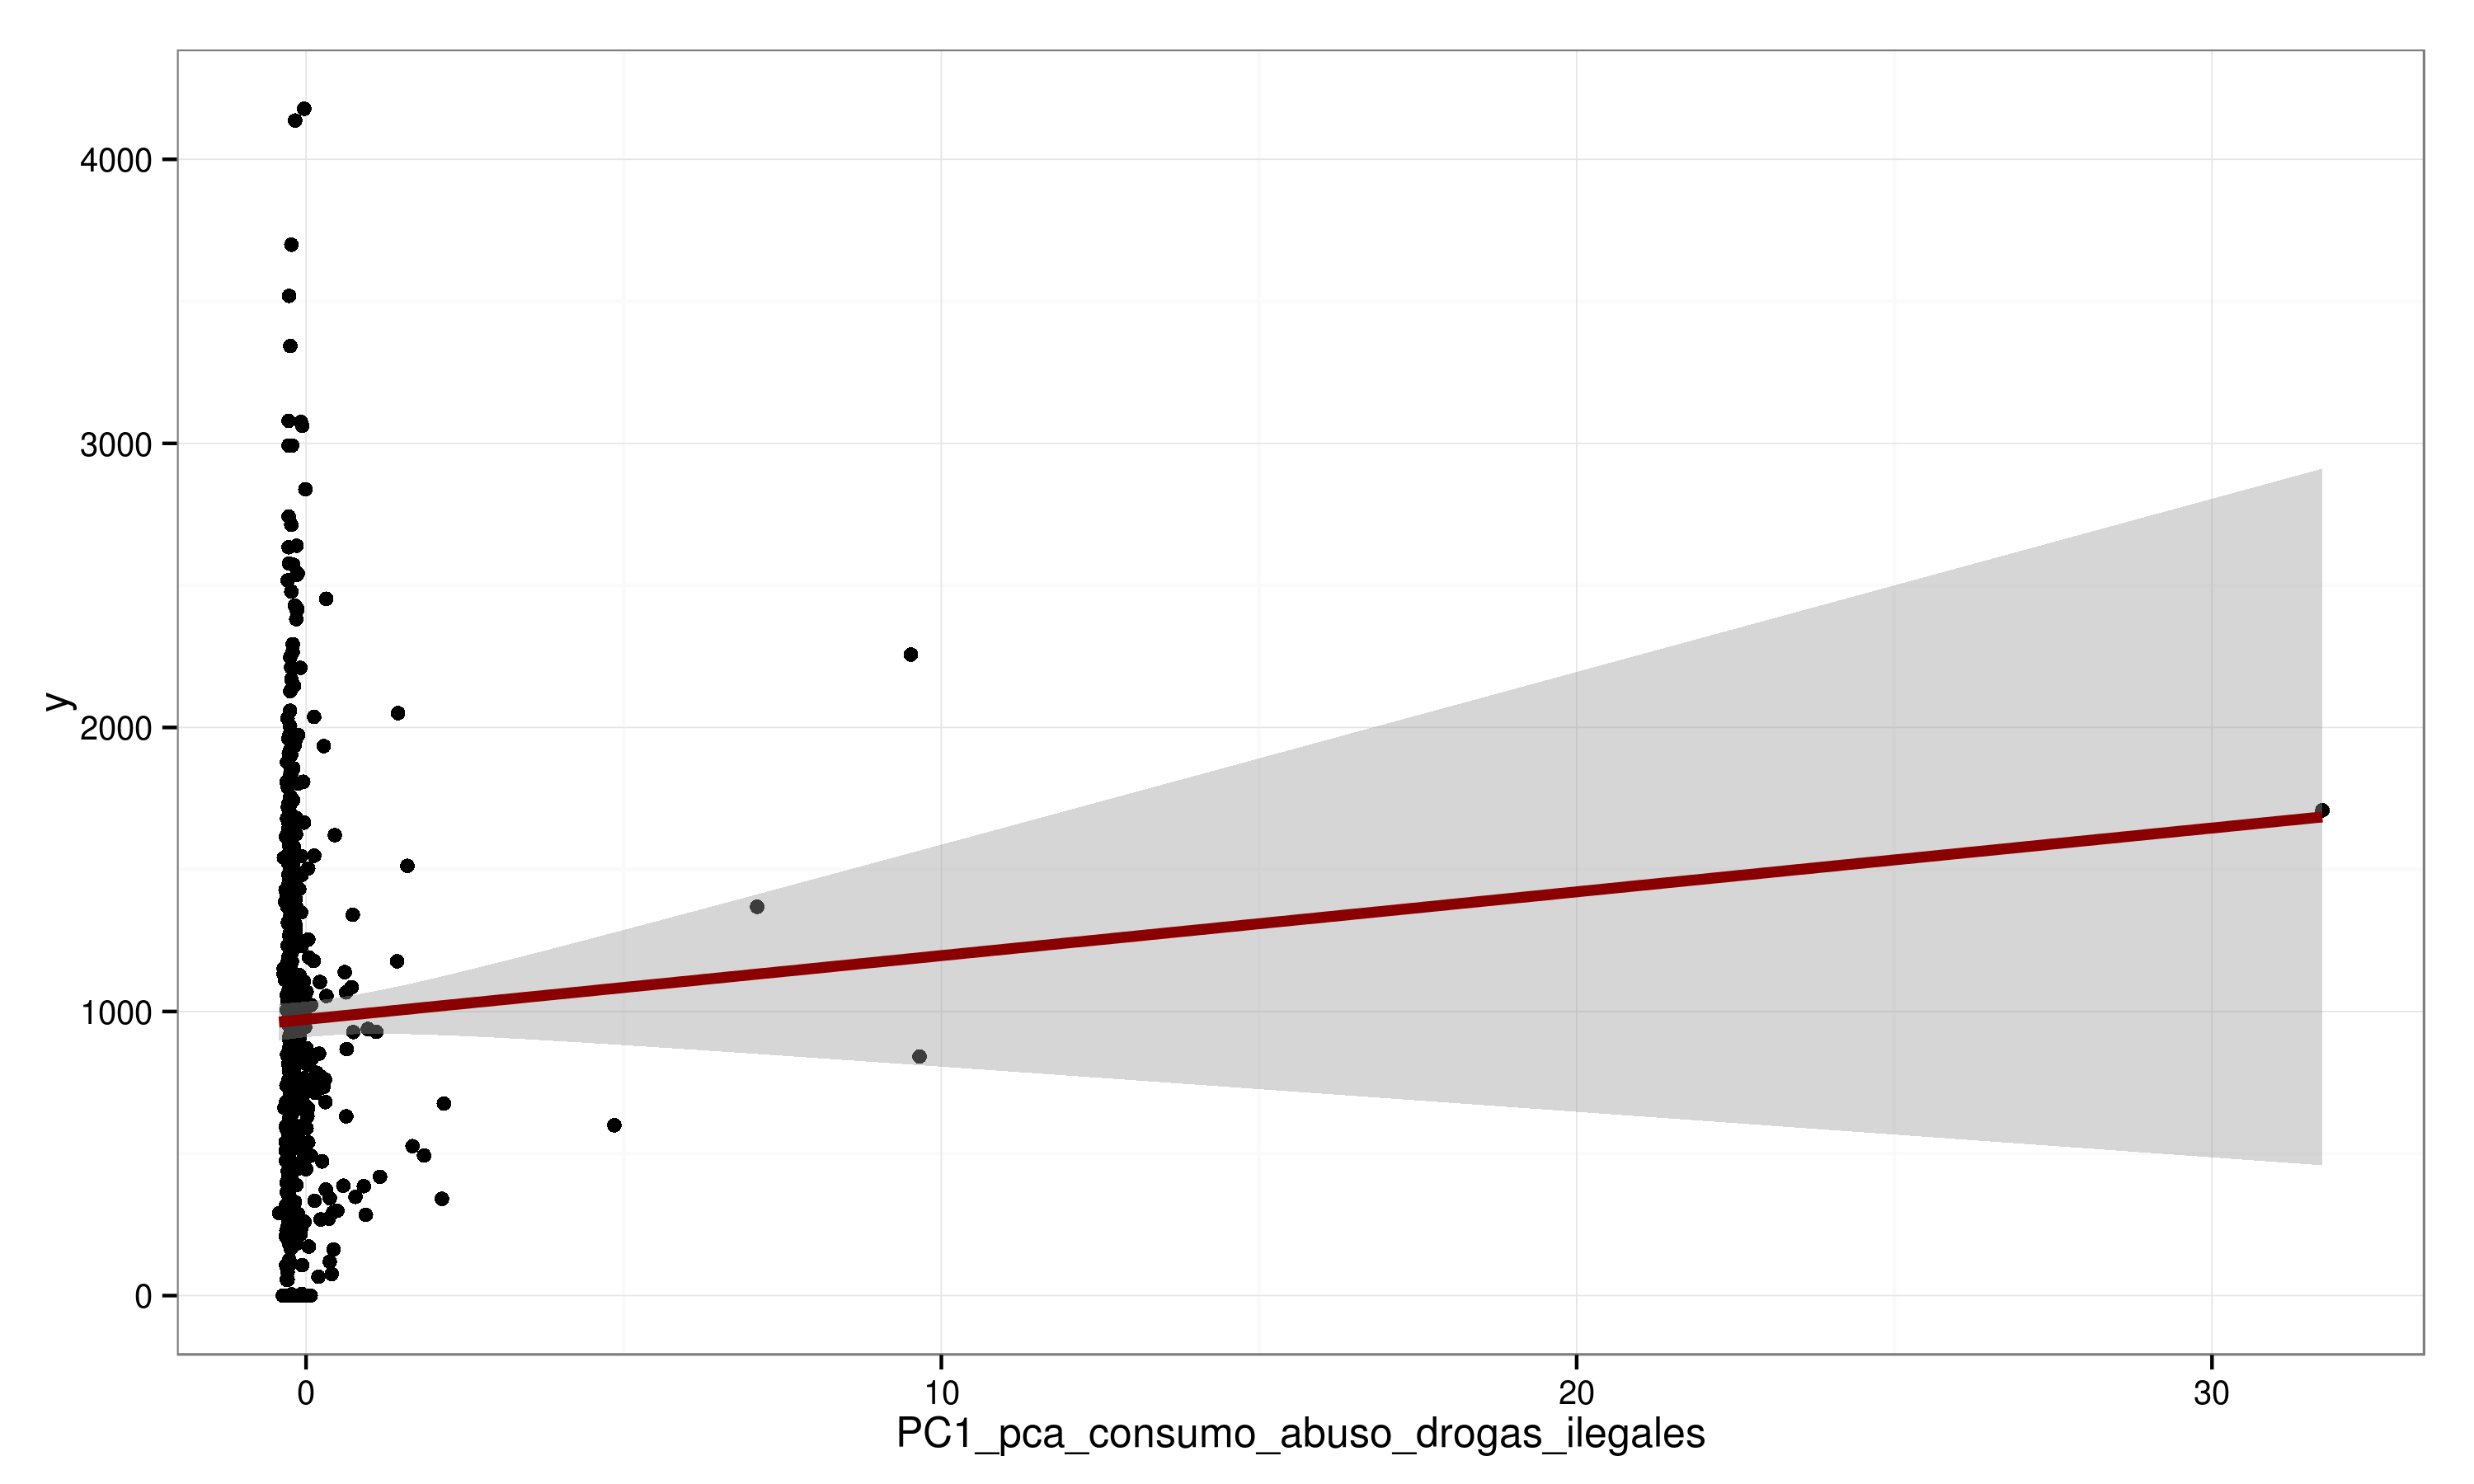
\includegraphics{img/y_indep13.png}

\end{frame}

\begin{frame}{Outliers}

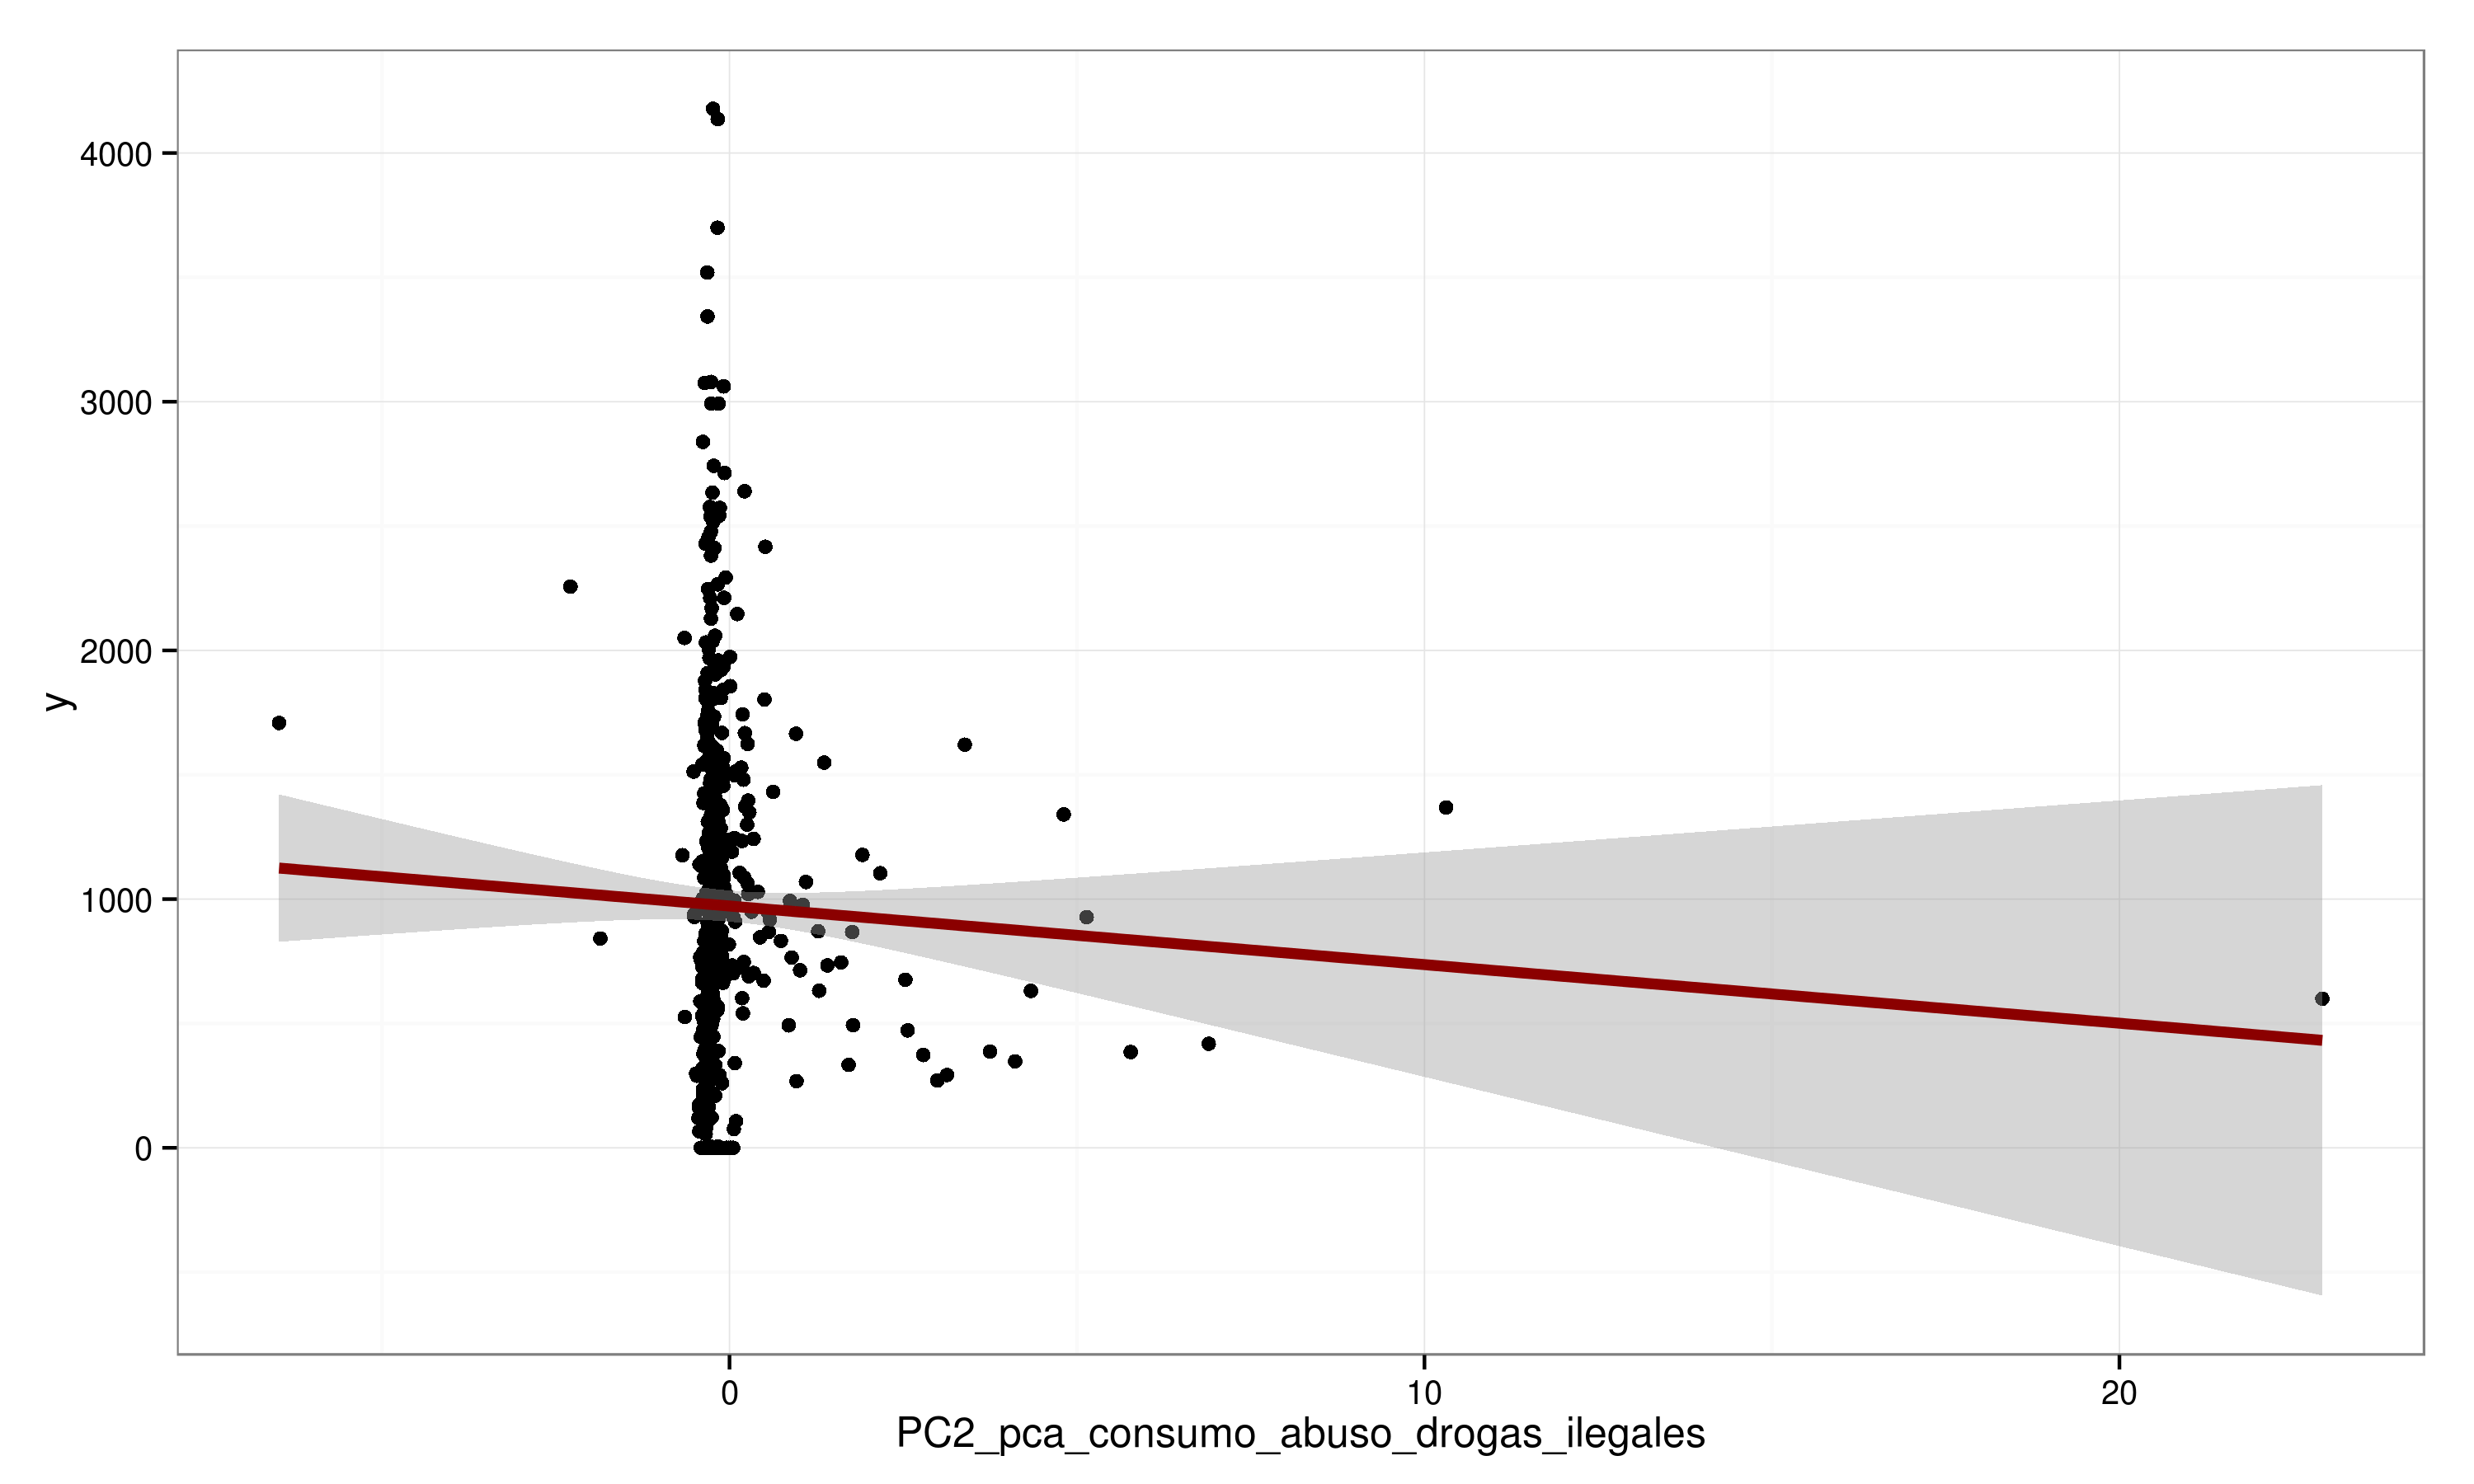
\includegraphics{img/y_indep21.png}

\end{frame}

\begin{frame}{Outliers}

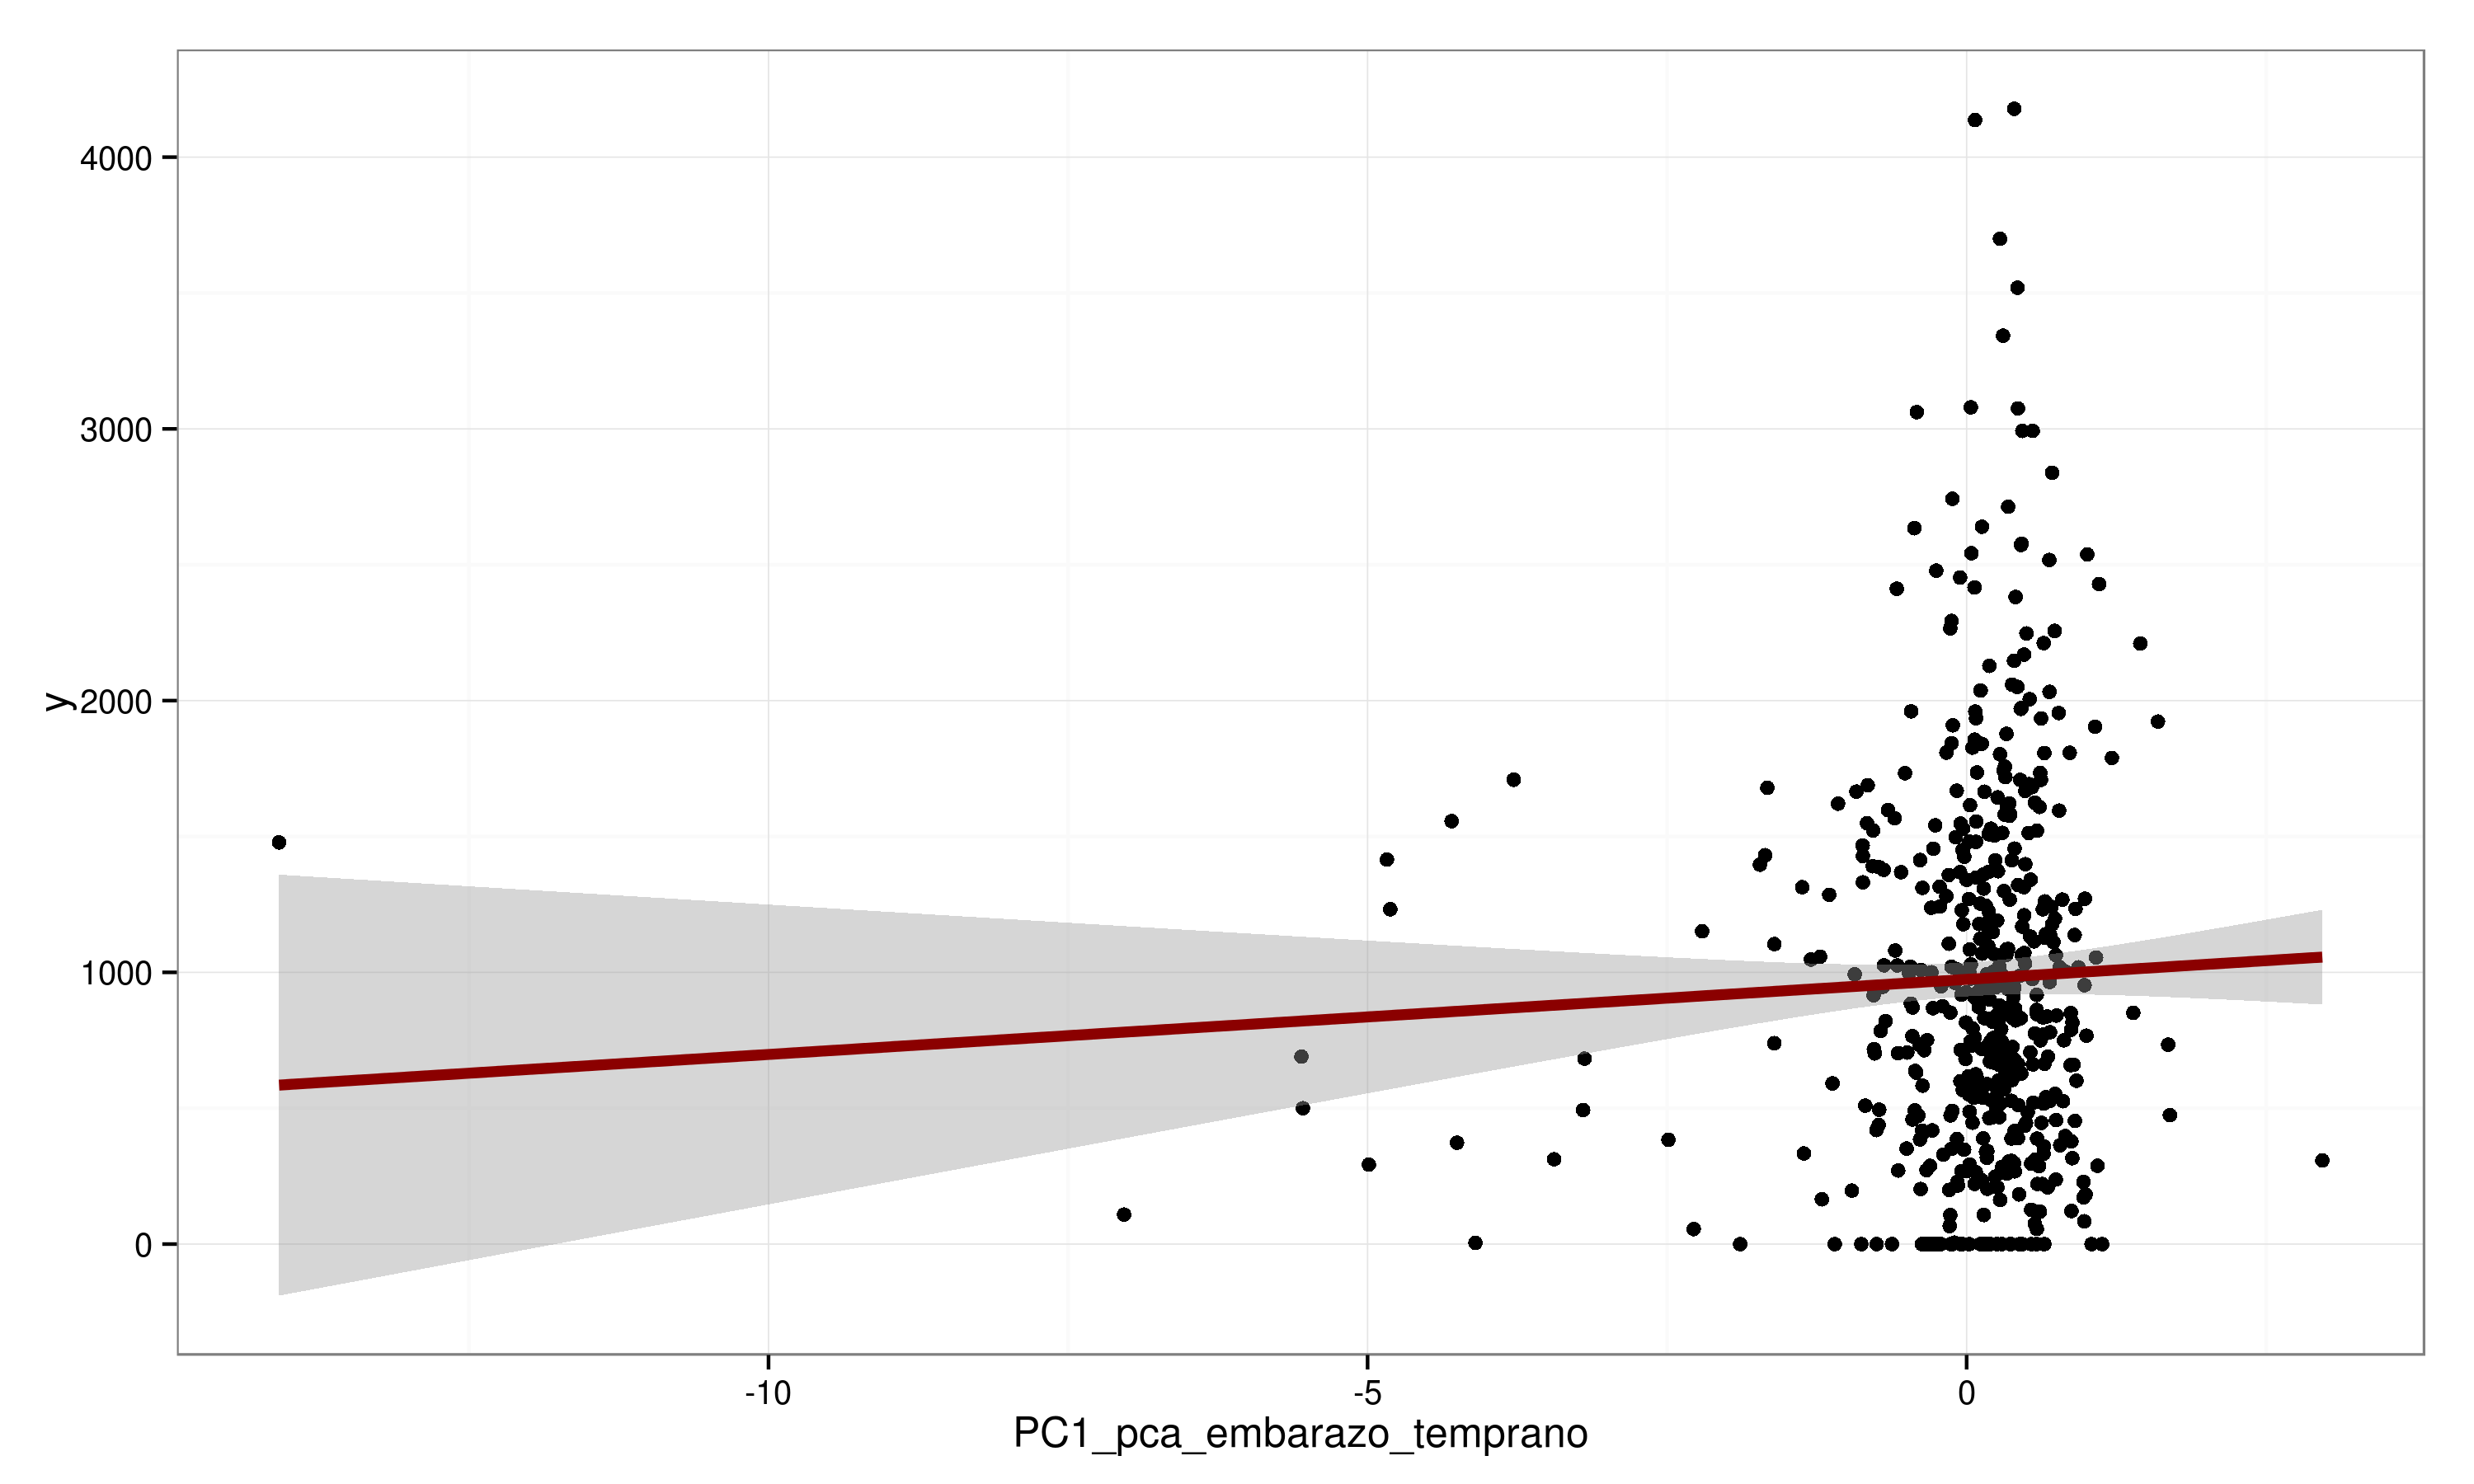
\includegraphics{img/y_indep15.png}

\end{frame}

\begin{frame}{Outliers}

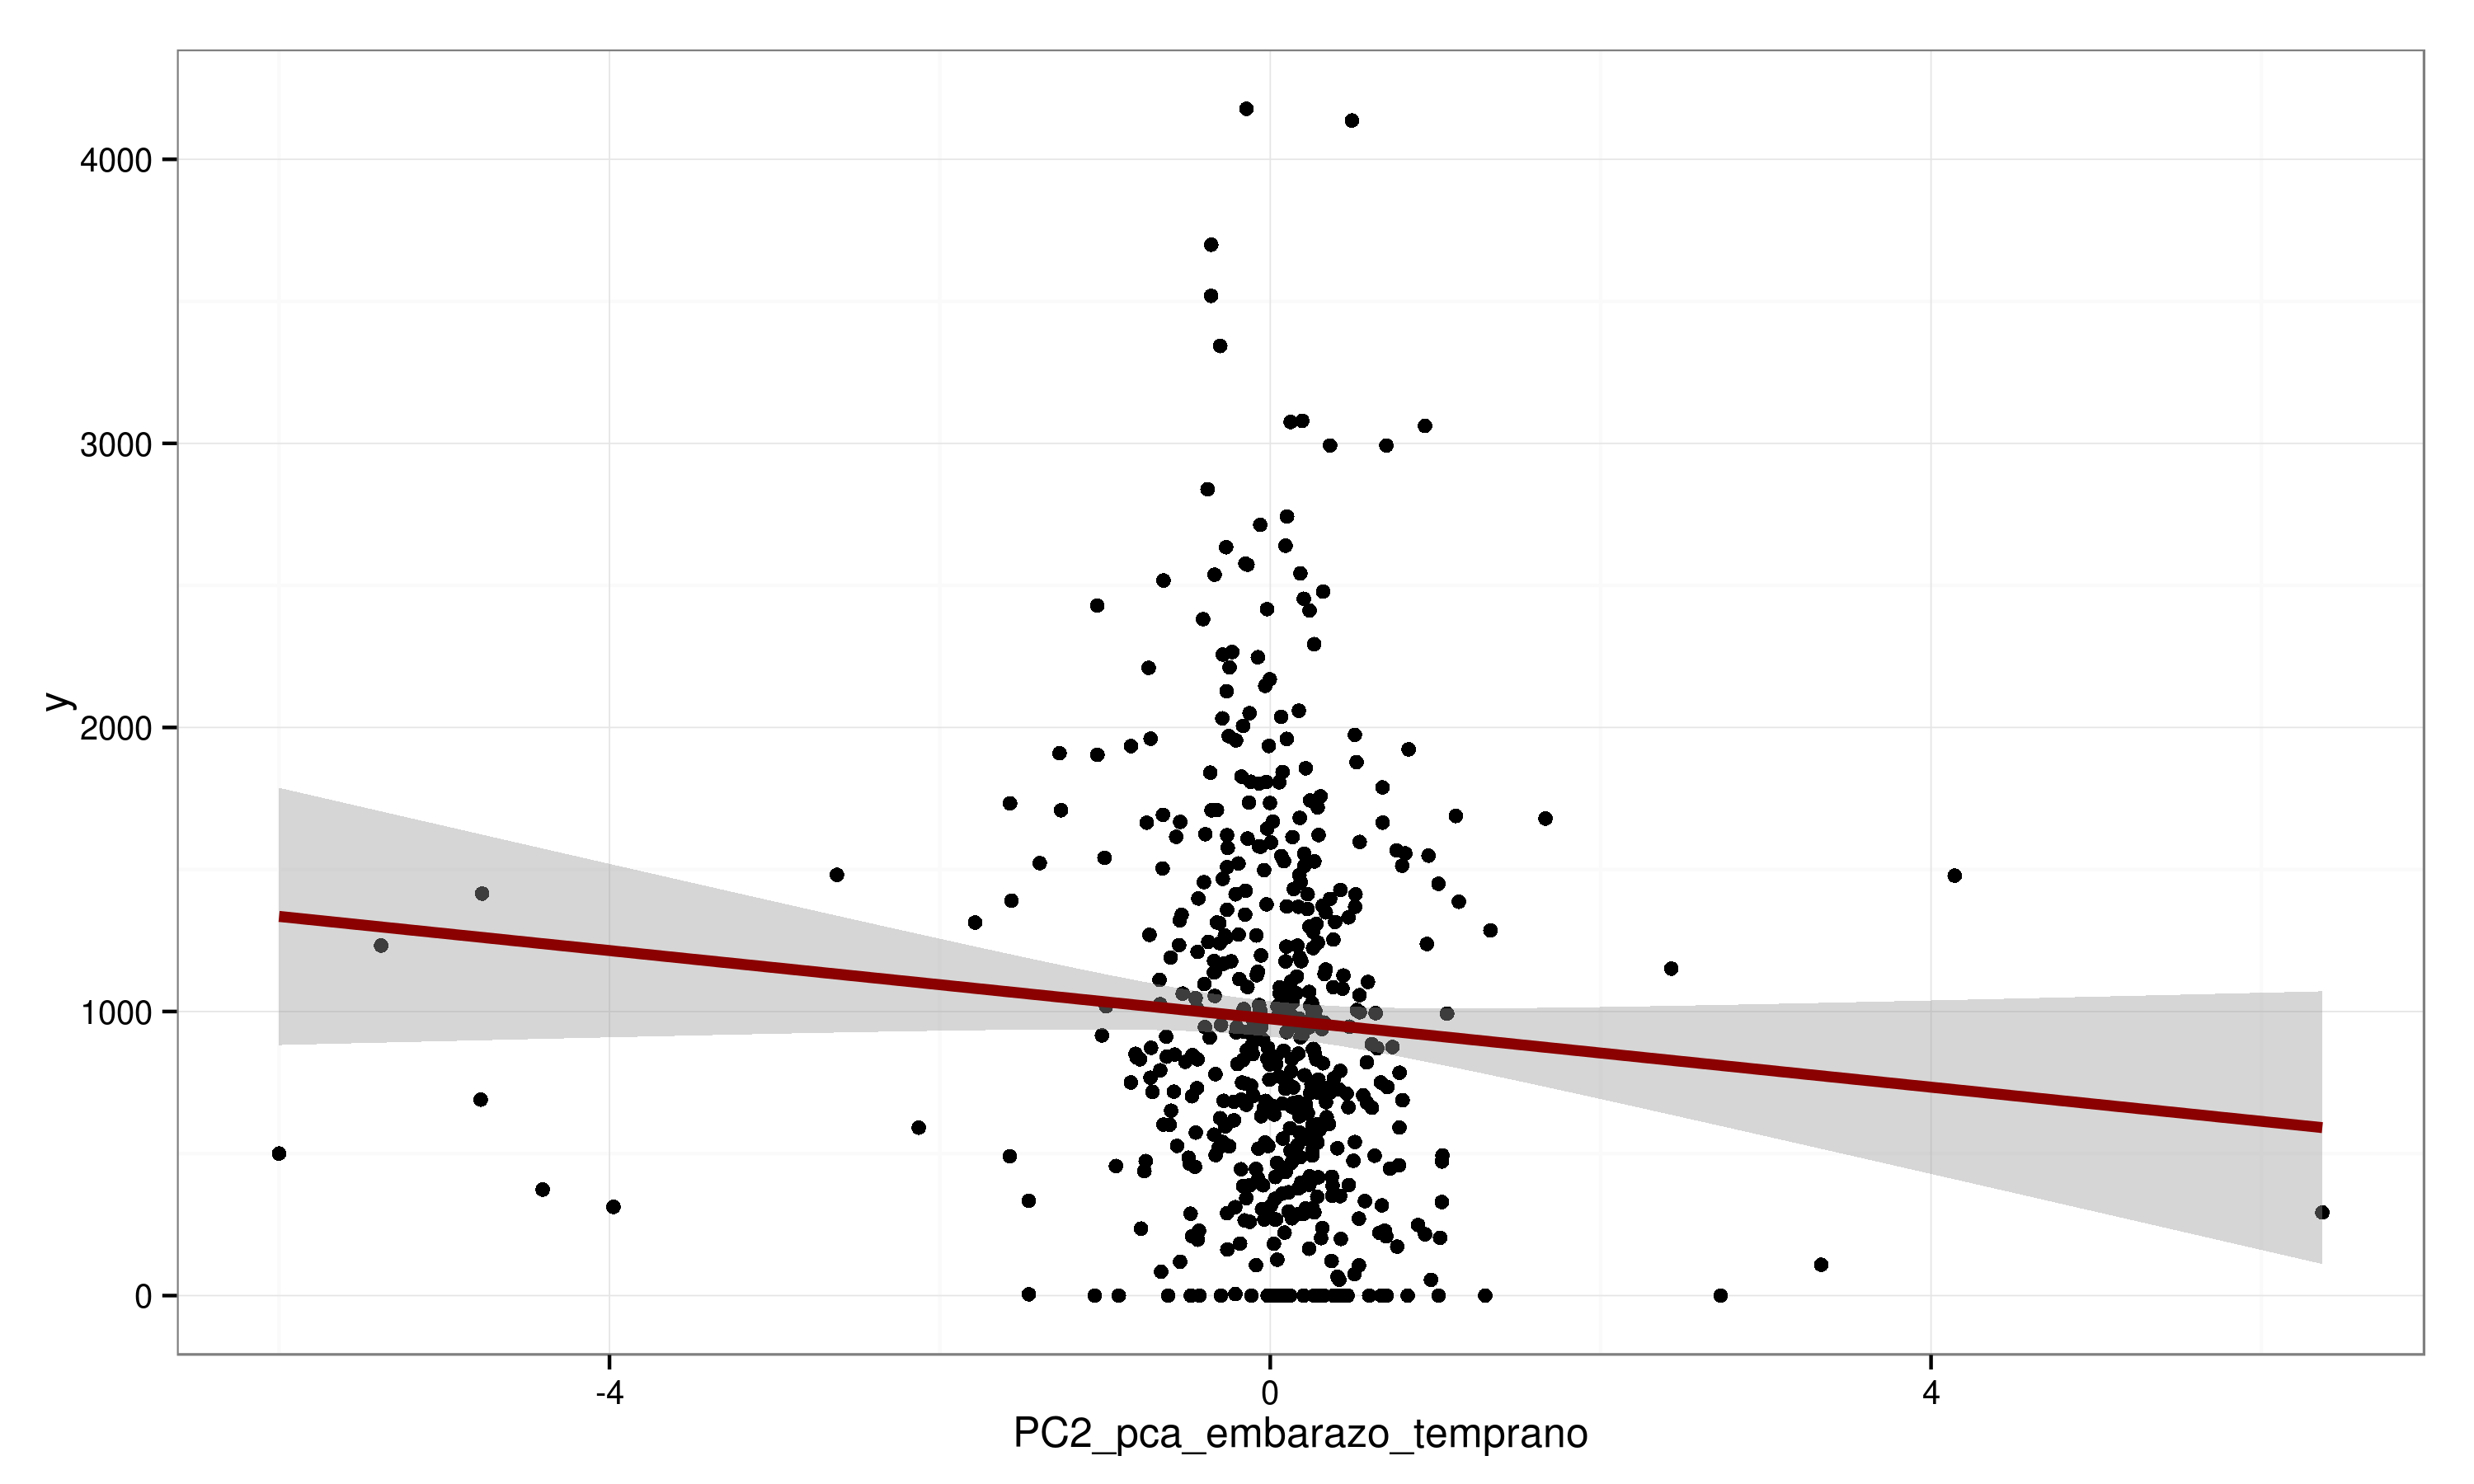
\includegraphics{img/y_indep23.png}

\end{frame}

\begin{frame}{Outliers}

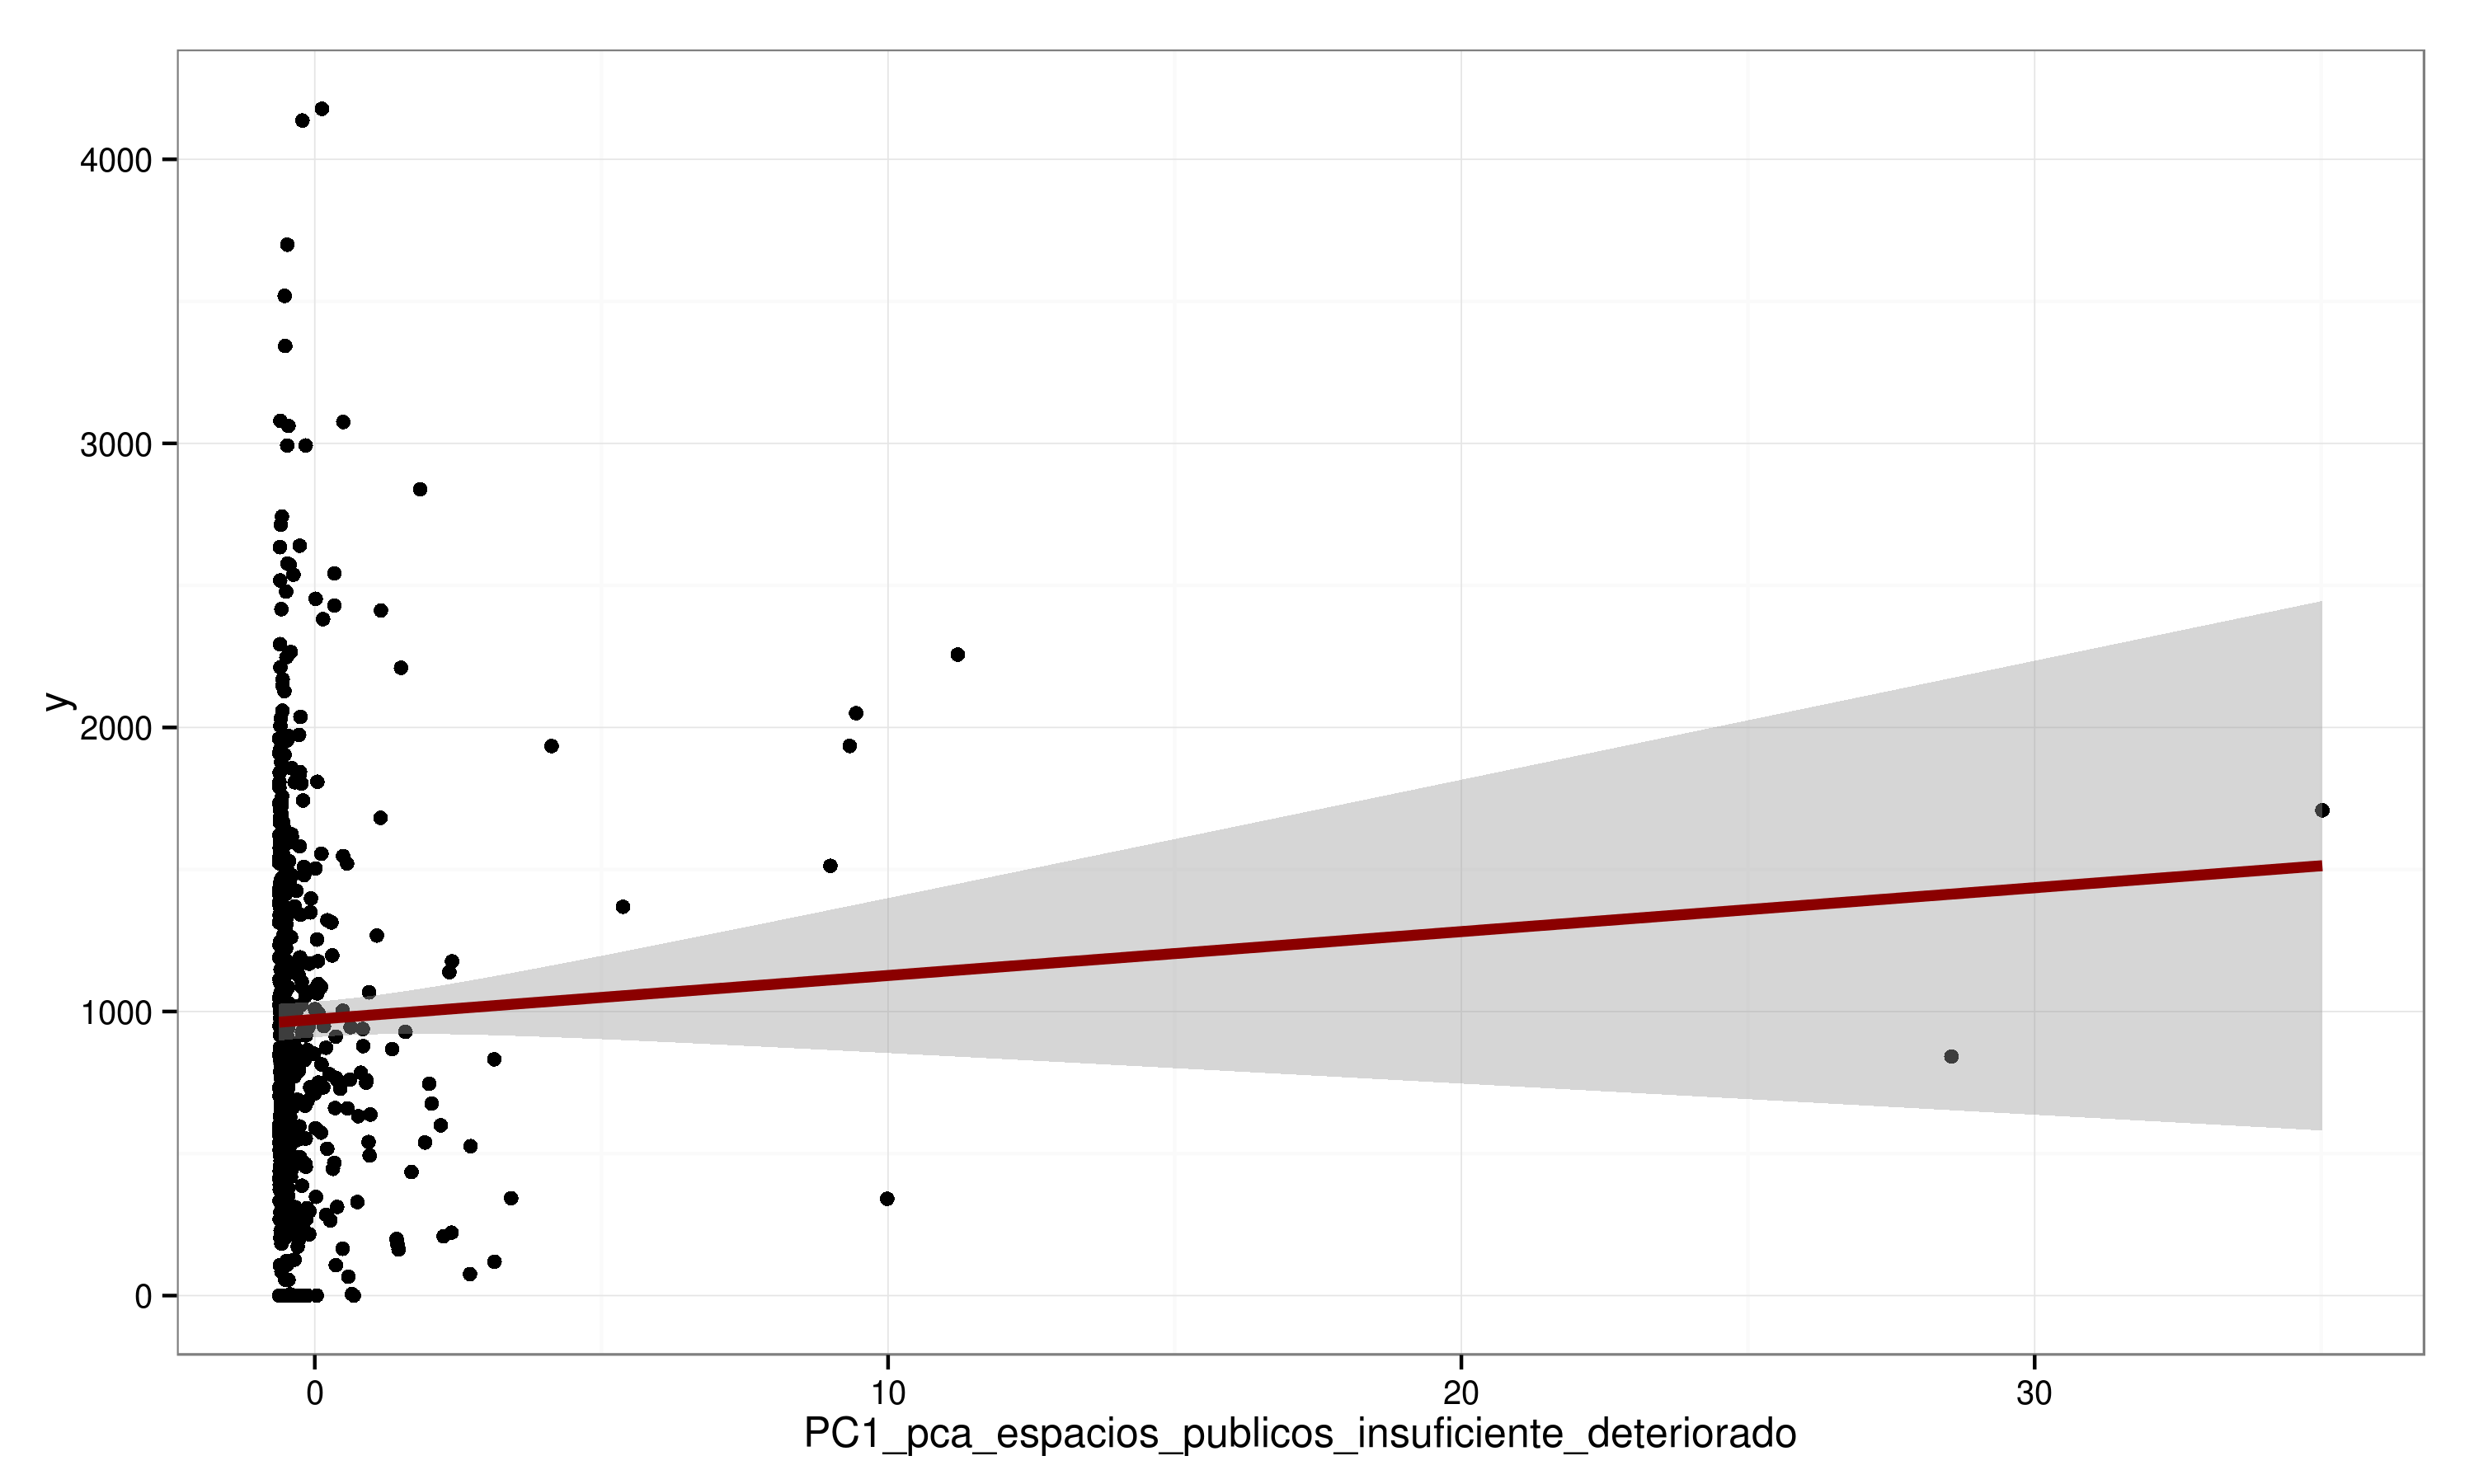
\includegraphics{img/y_indep16.png}

\end{frame}

\begin{frame}{Outliers}

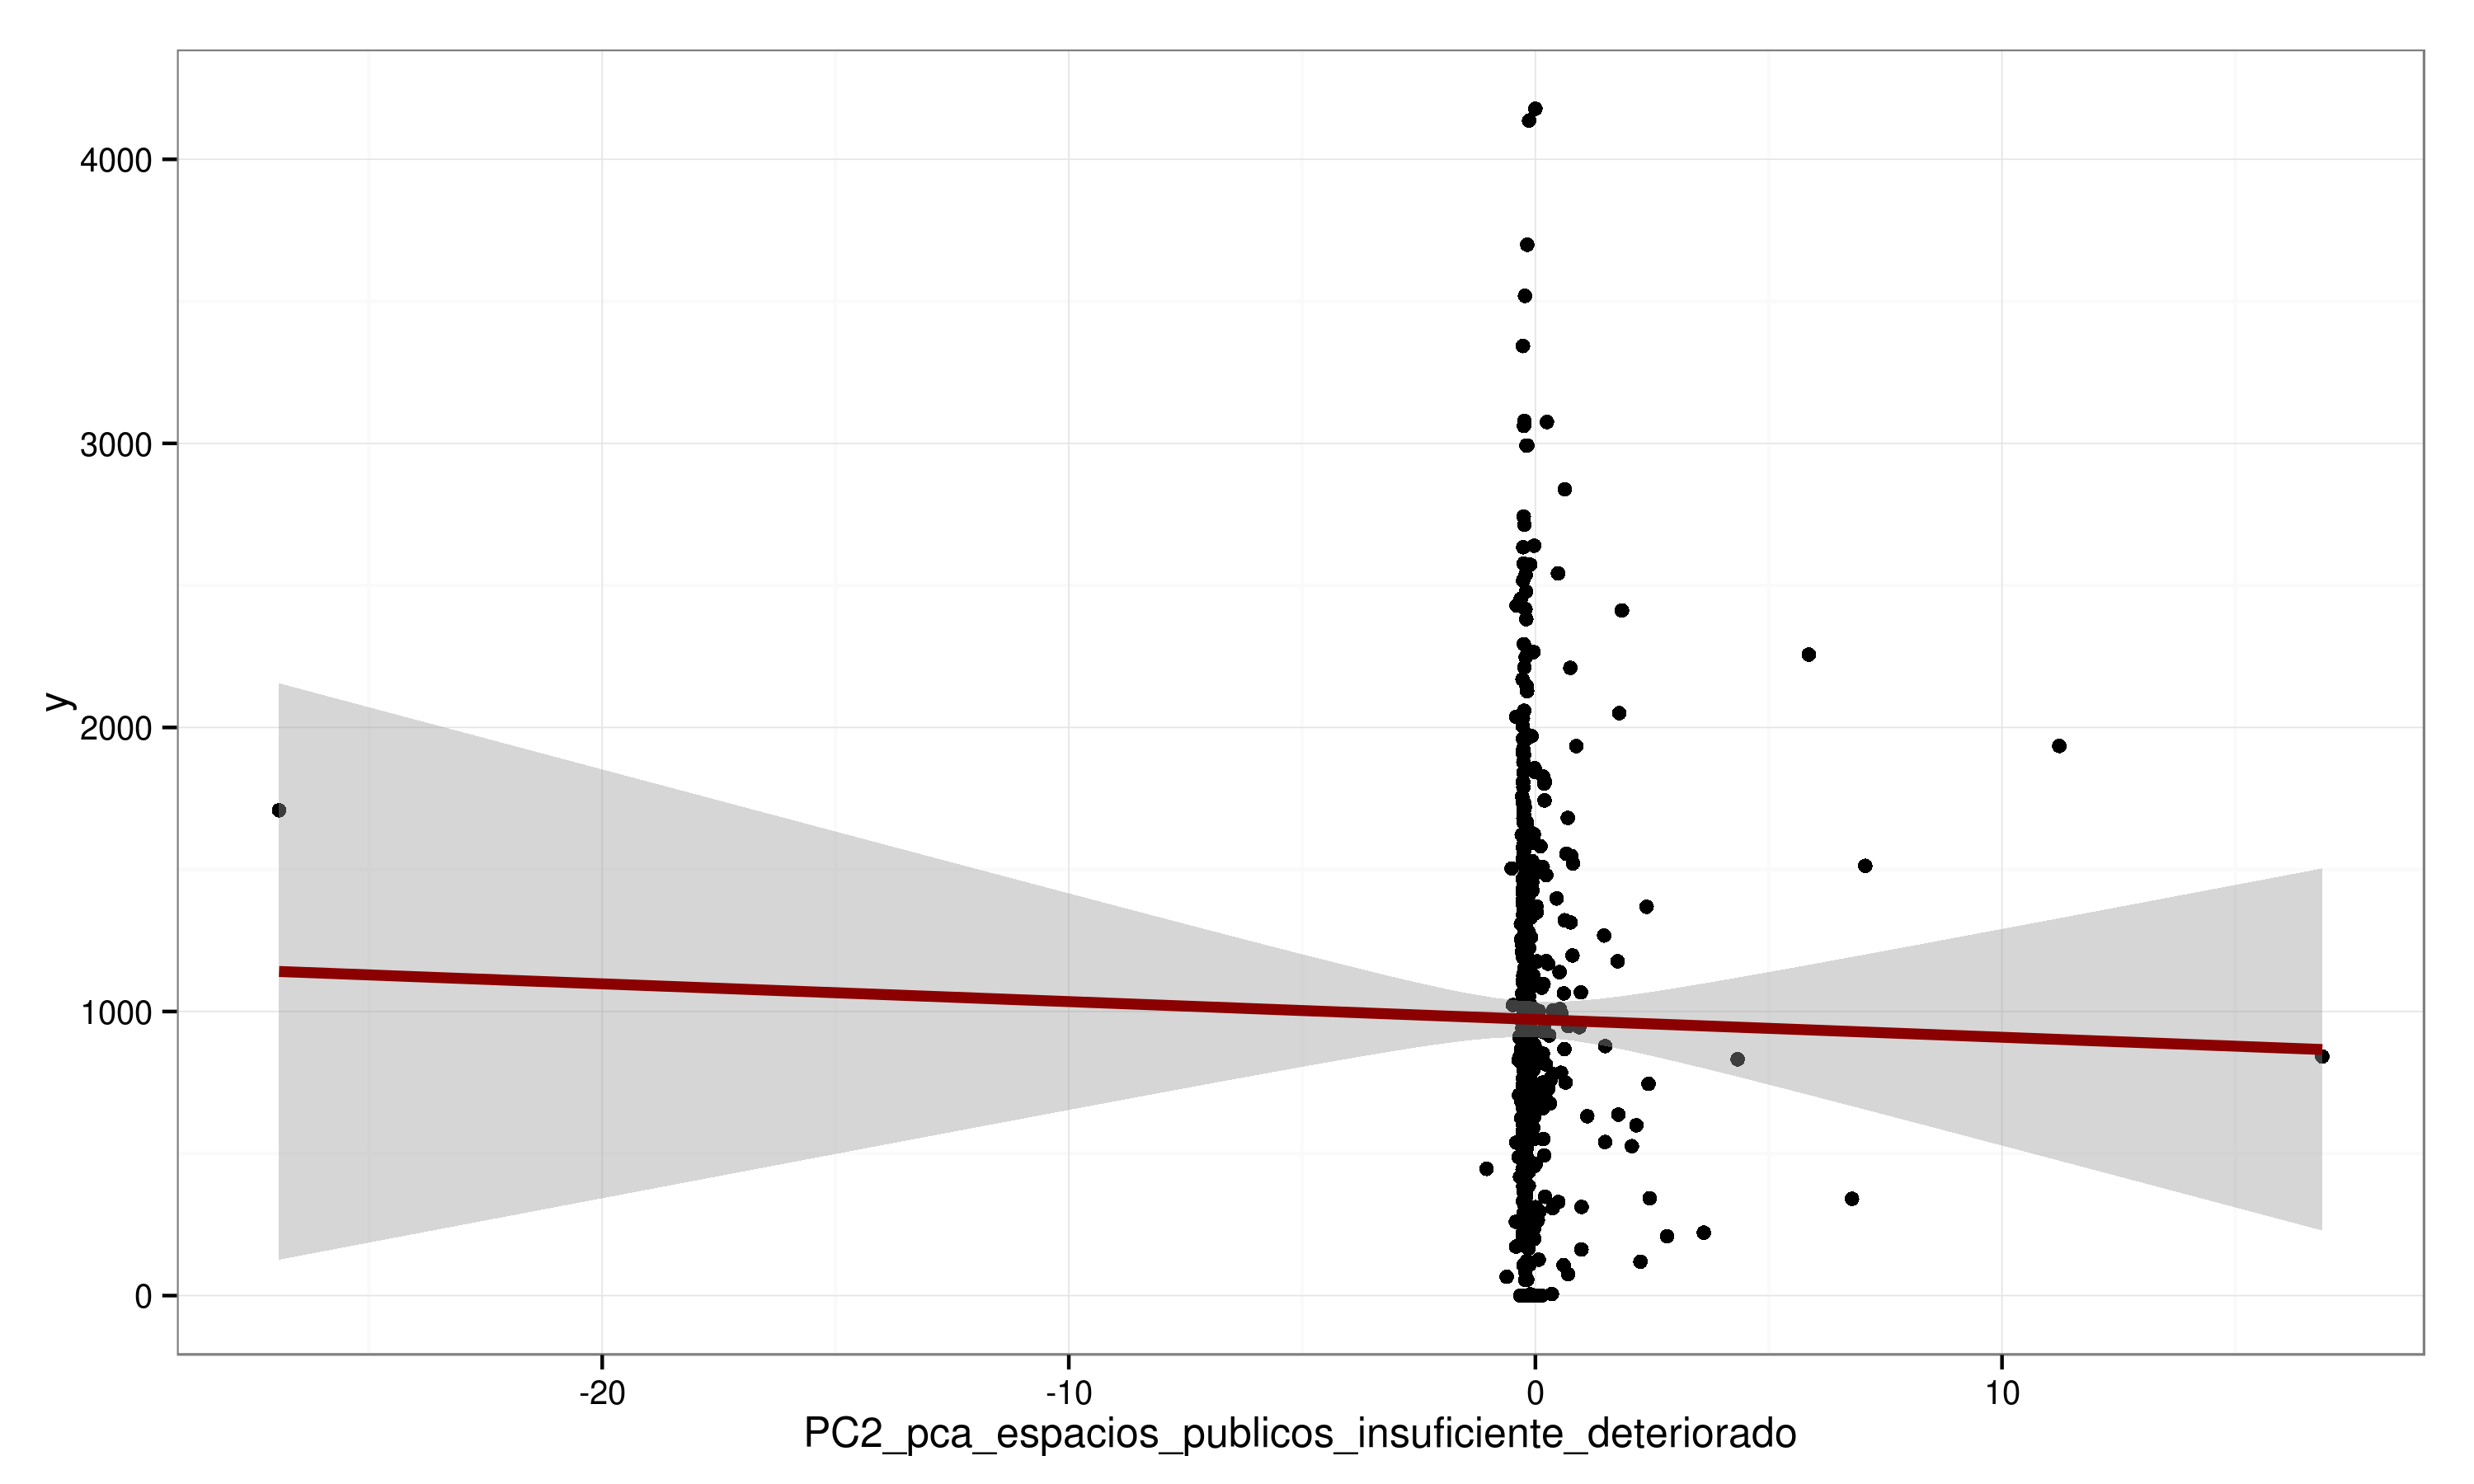
\includegraphics{img/y_indep24.png}

\end{frame}

\begin{frame}{Outliers}

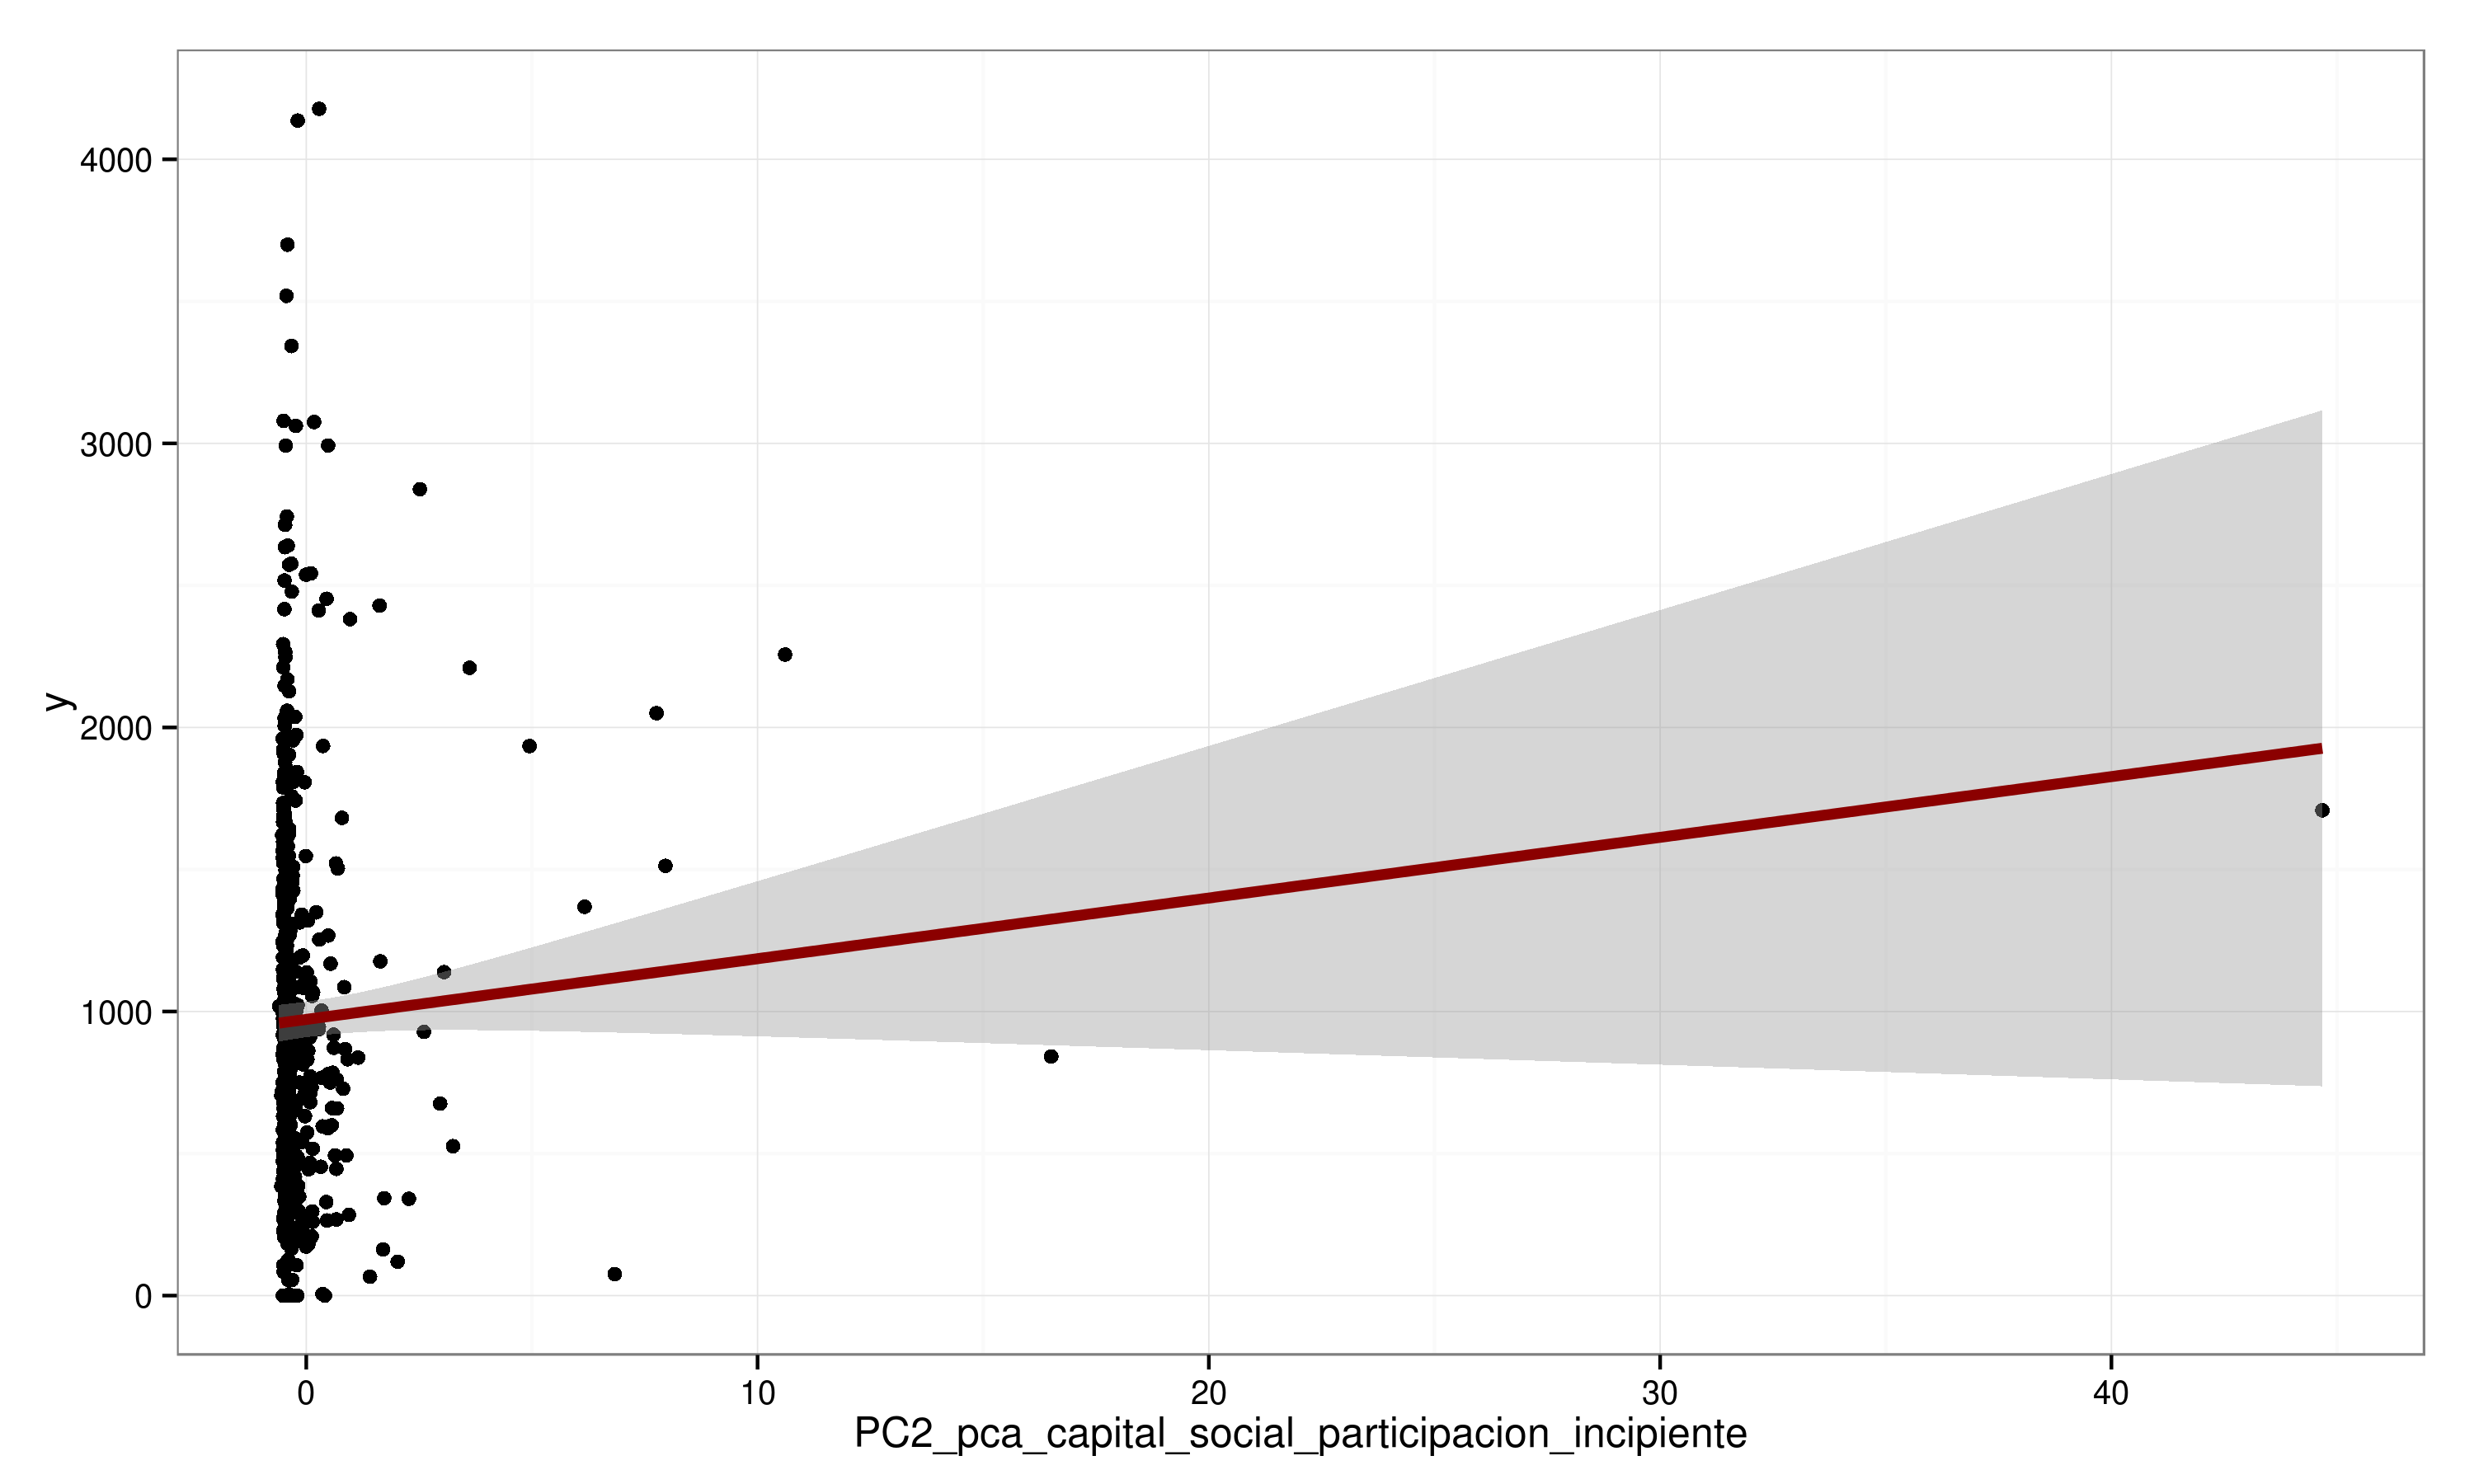
\includegraphics{img/y_indep20.png}

\end{frame}

\begin{frame}{Factores de riesgo}

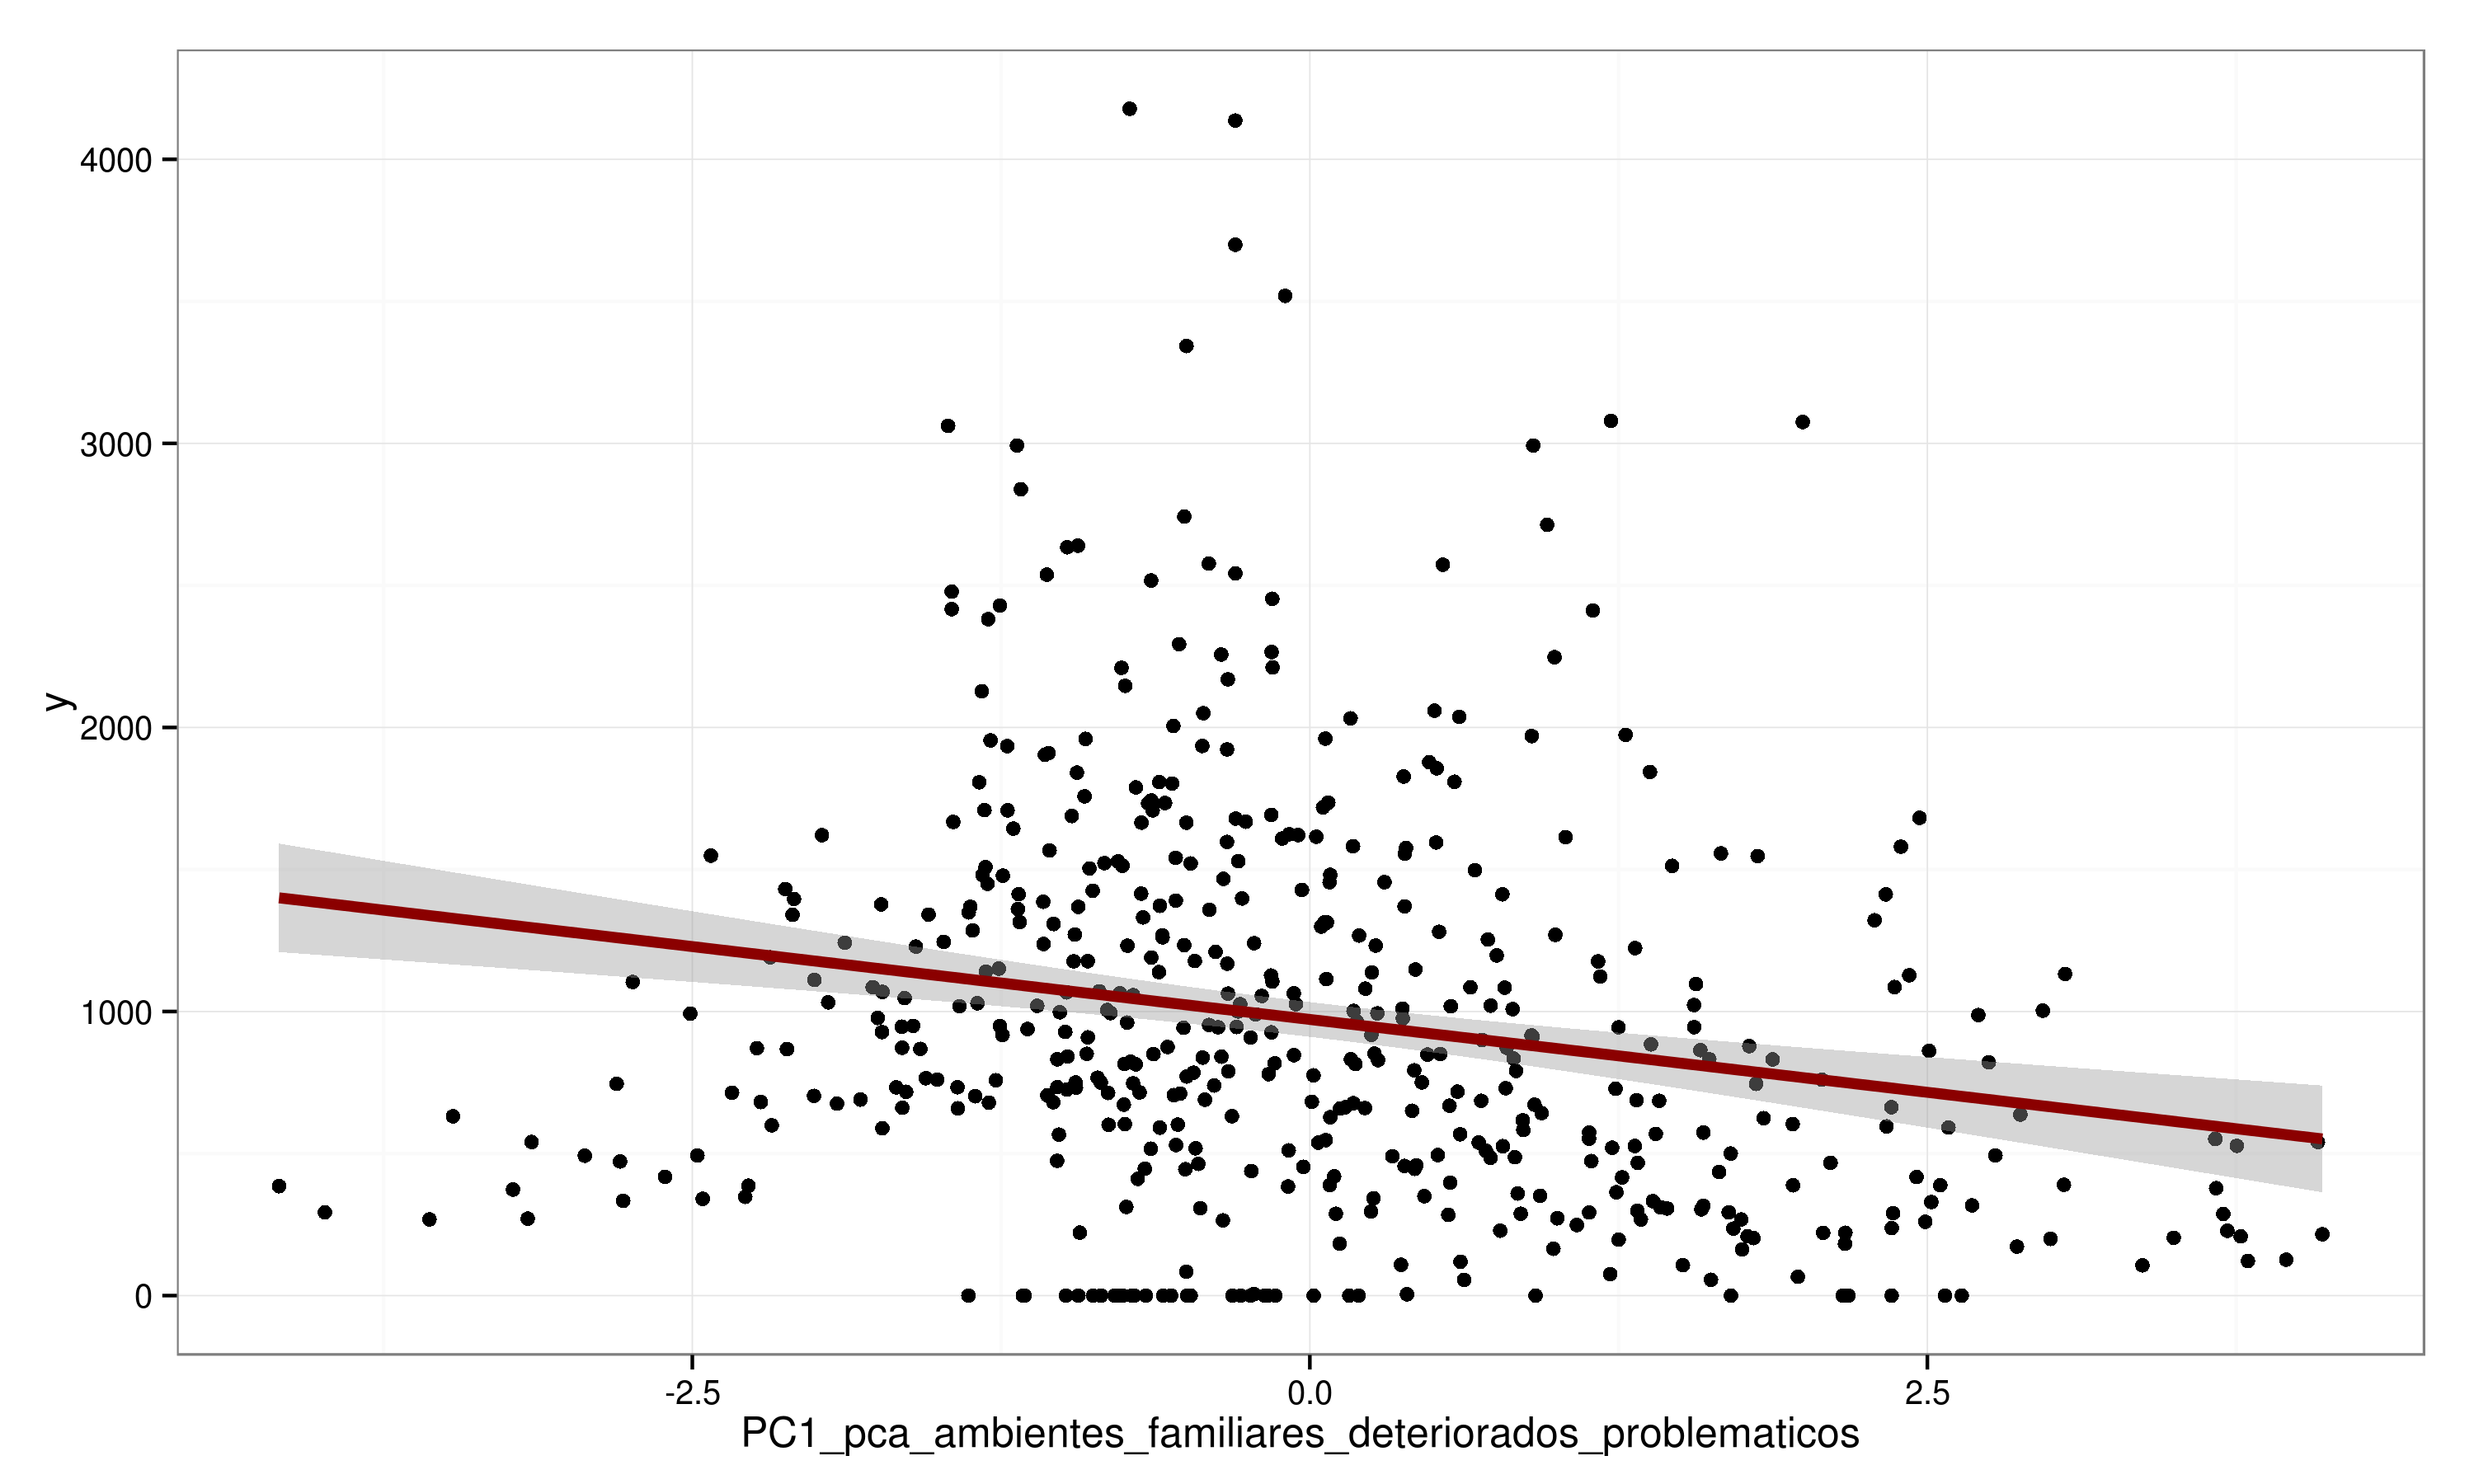
\includegraphics{img/y_indep11.png}

\end{frame}

\begin{frame}{Factores de riesgo}

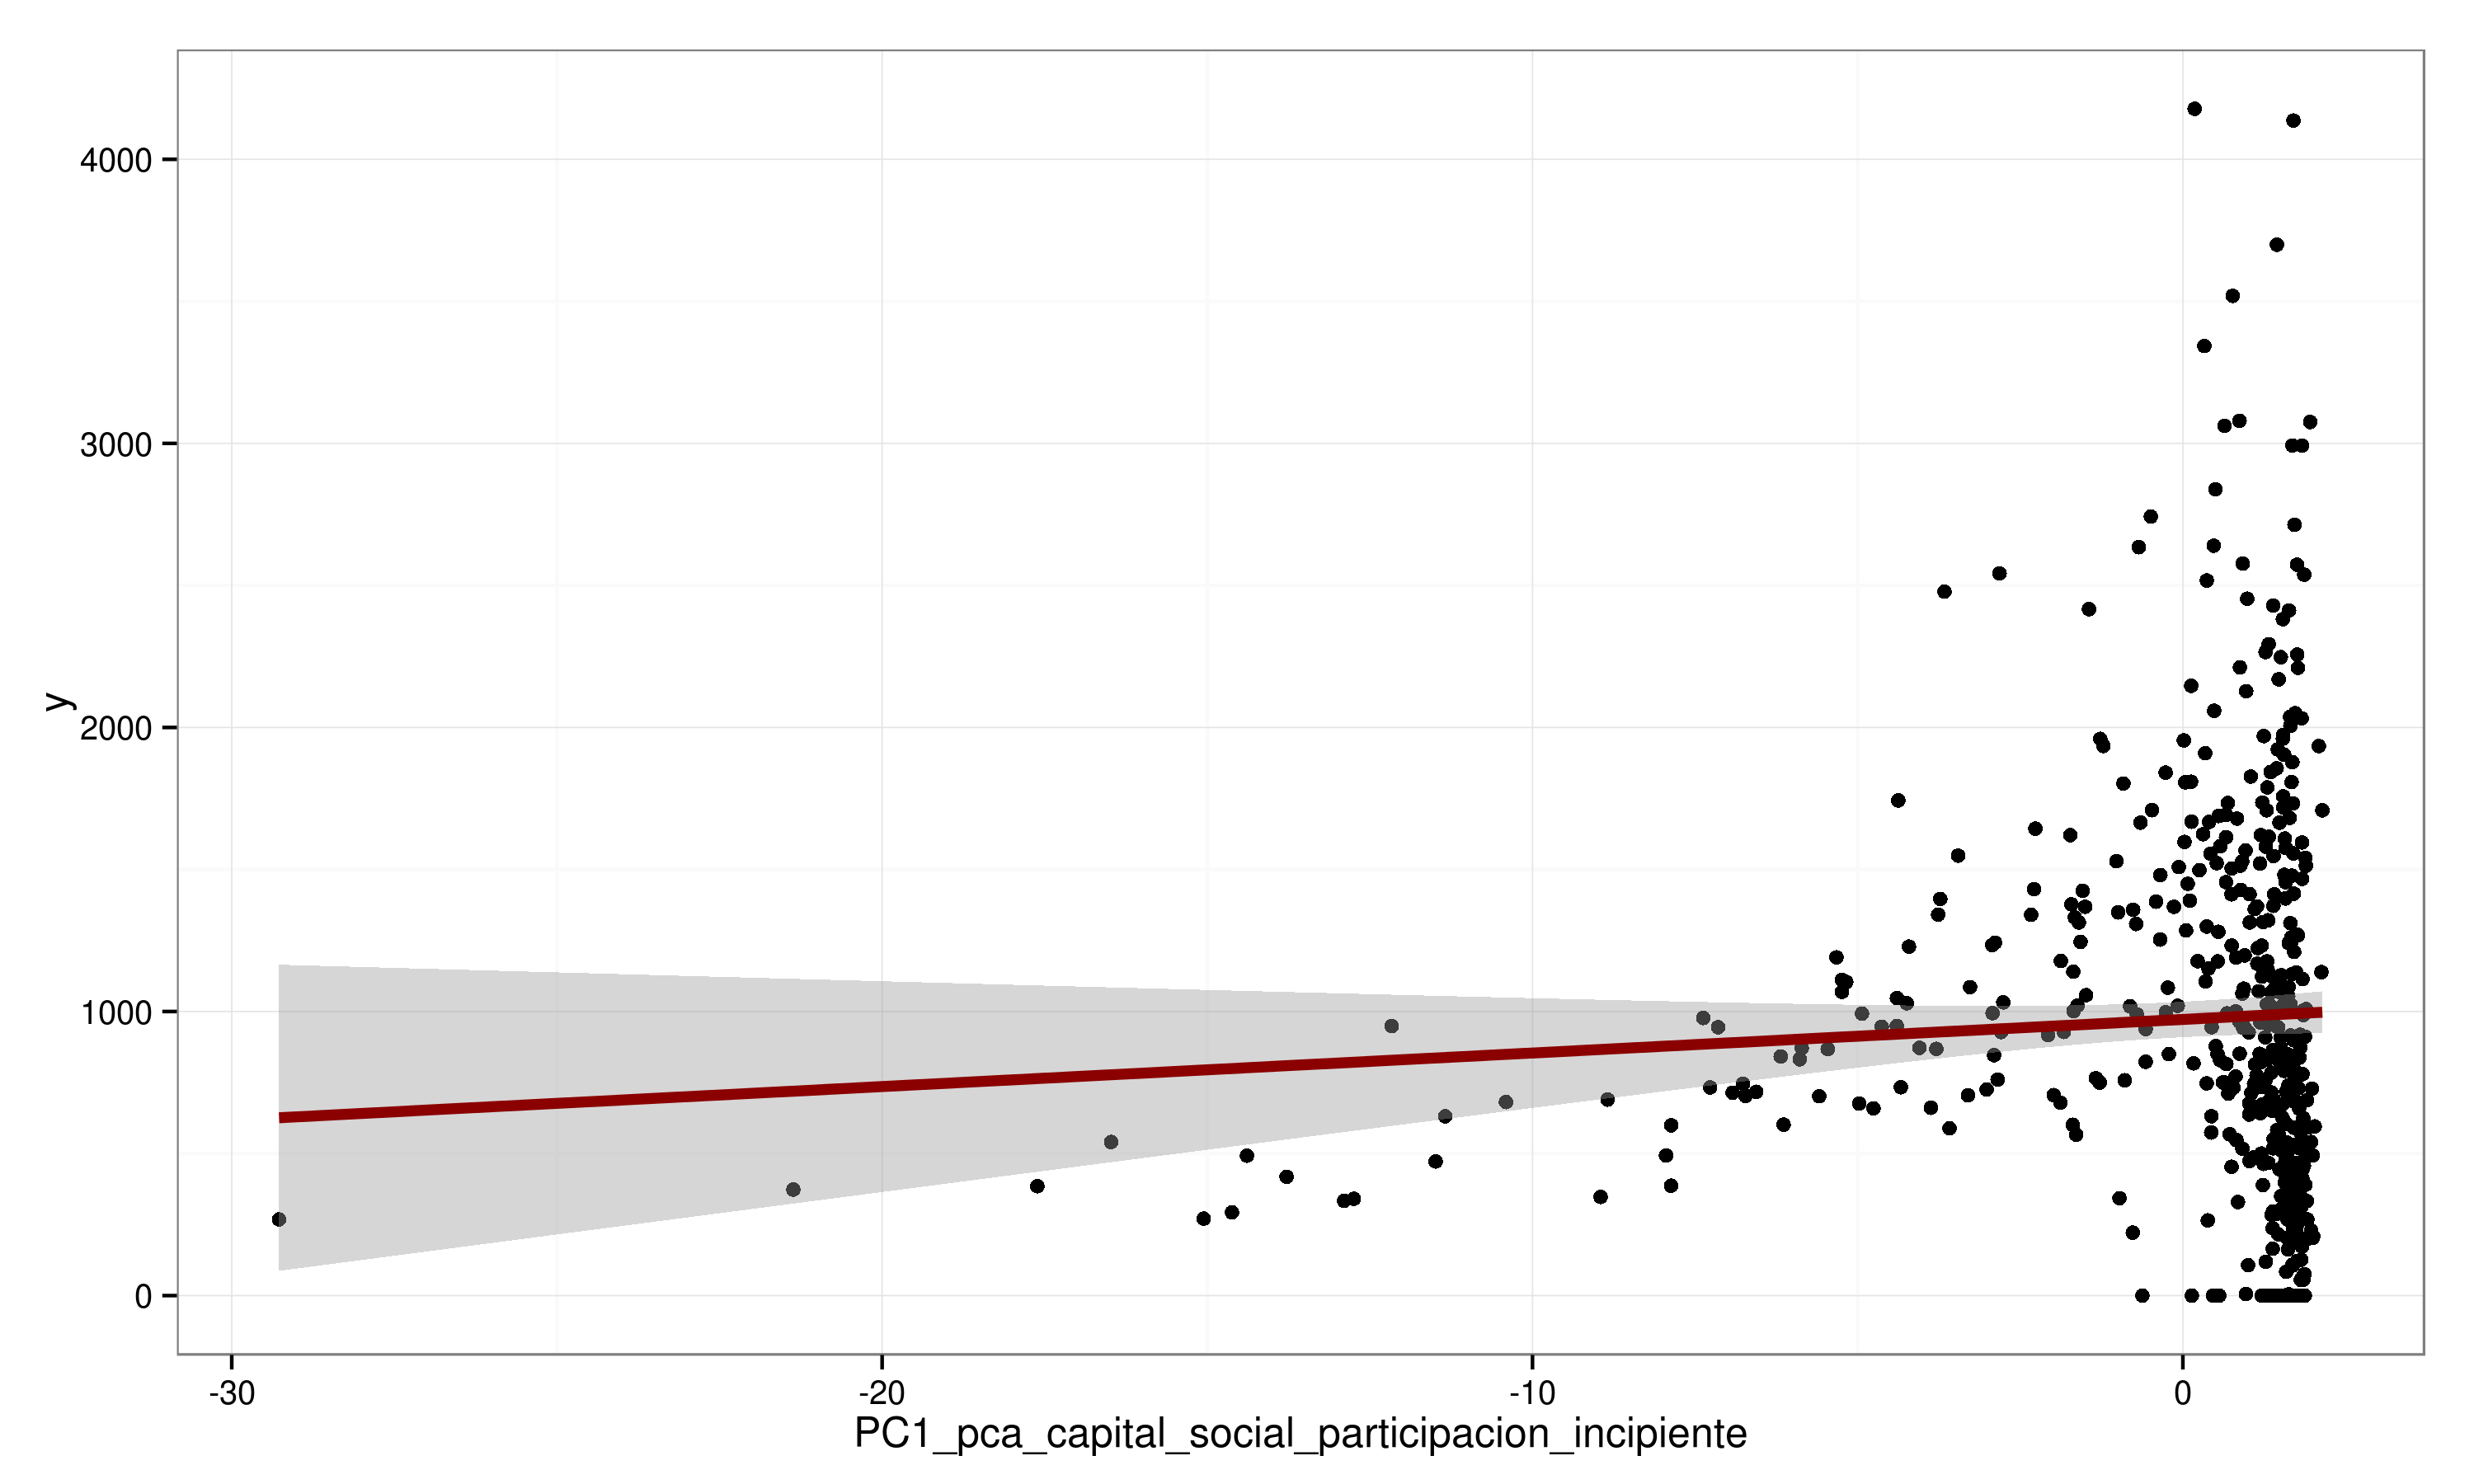
\includegraphics{img/y_indep12.png}

\end{frame}

\begin{frame}{Factores de riesgo}

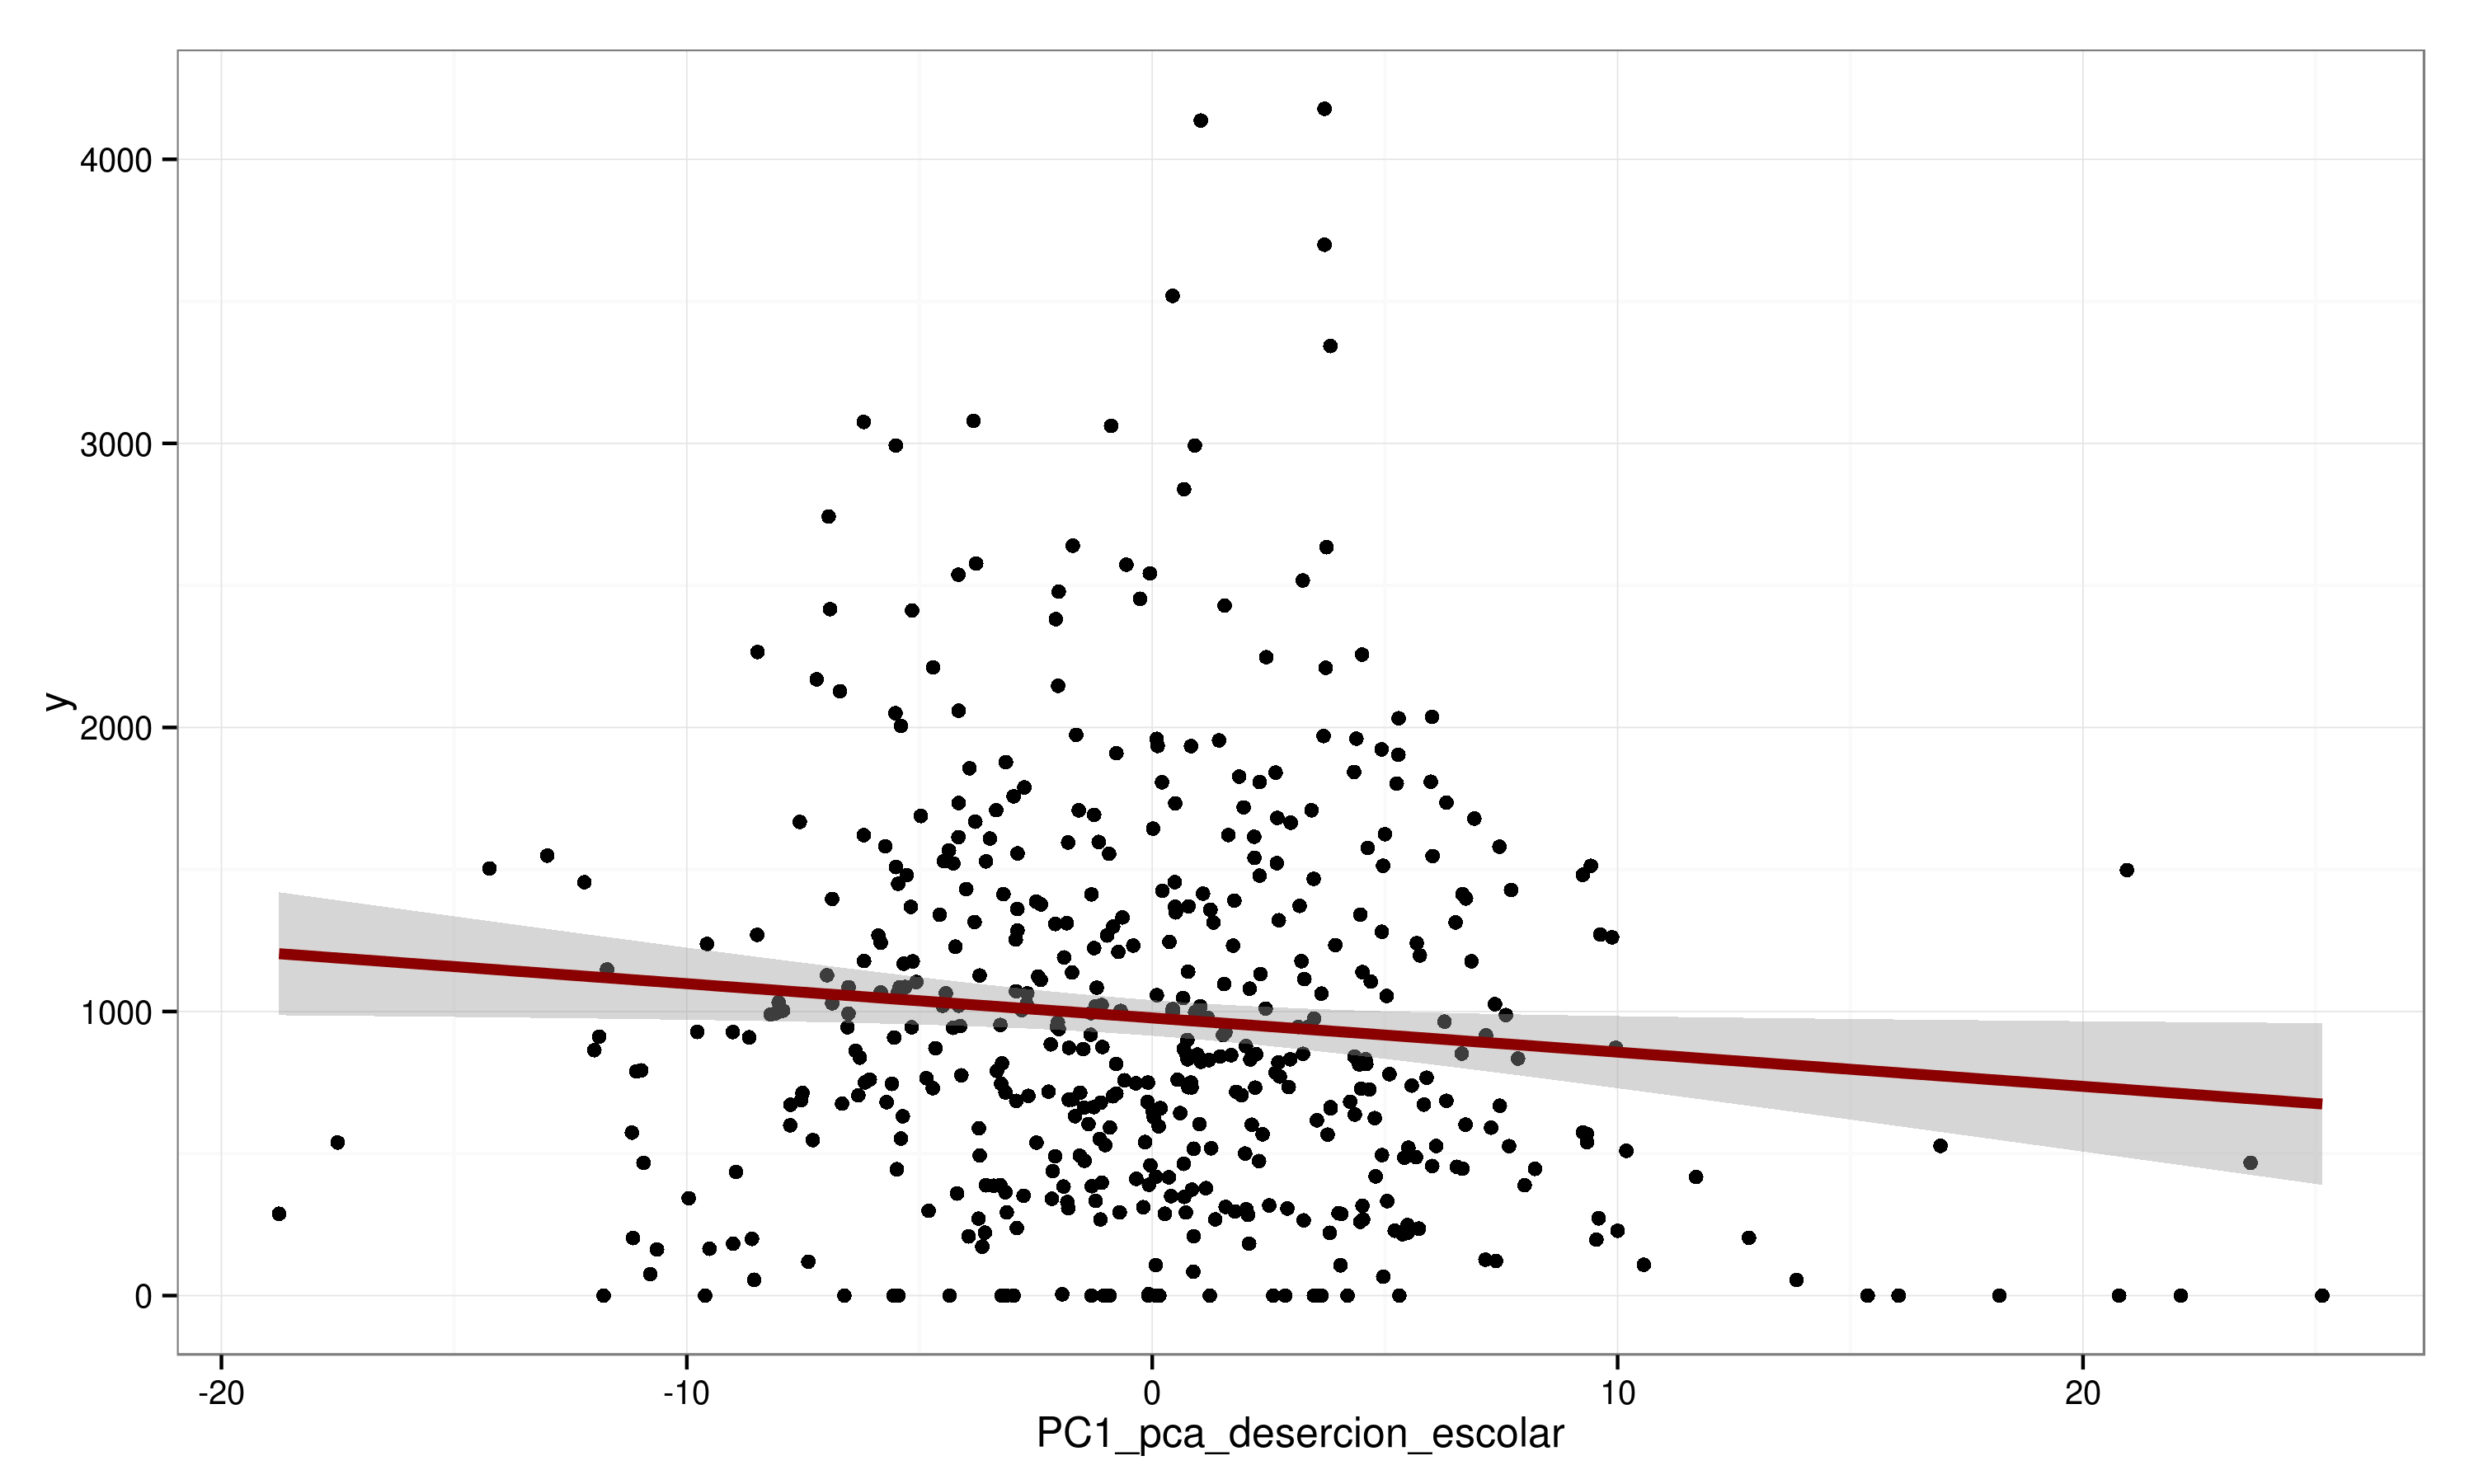
\includegraphics{img/y_indep14.png}

\end{frame}

\begin{frame}{Factores de riesgo}

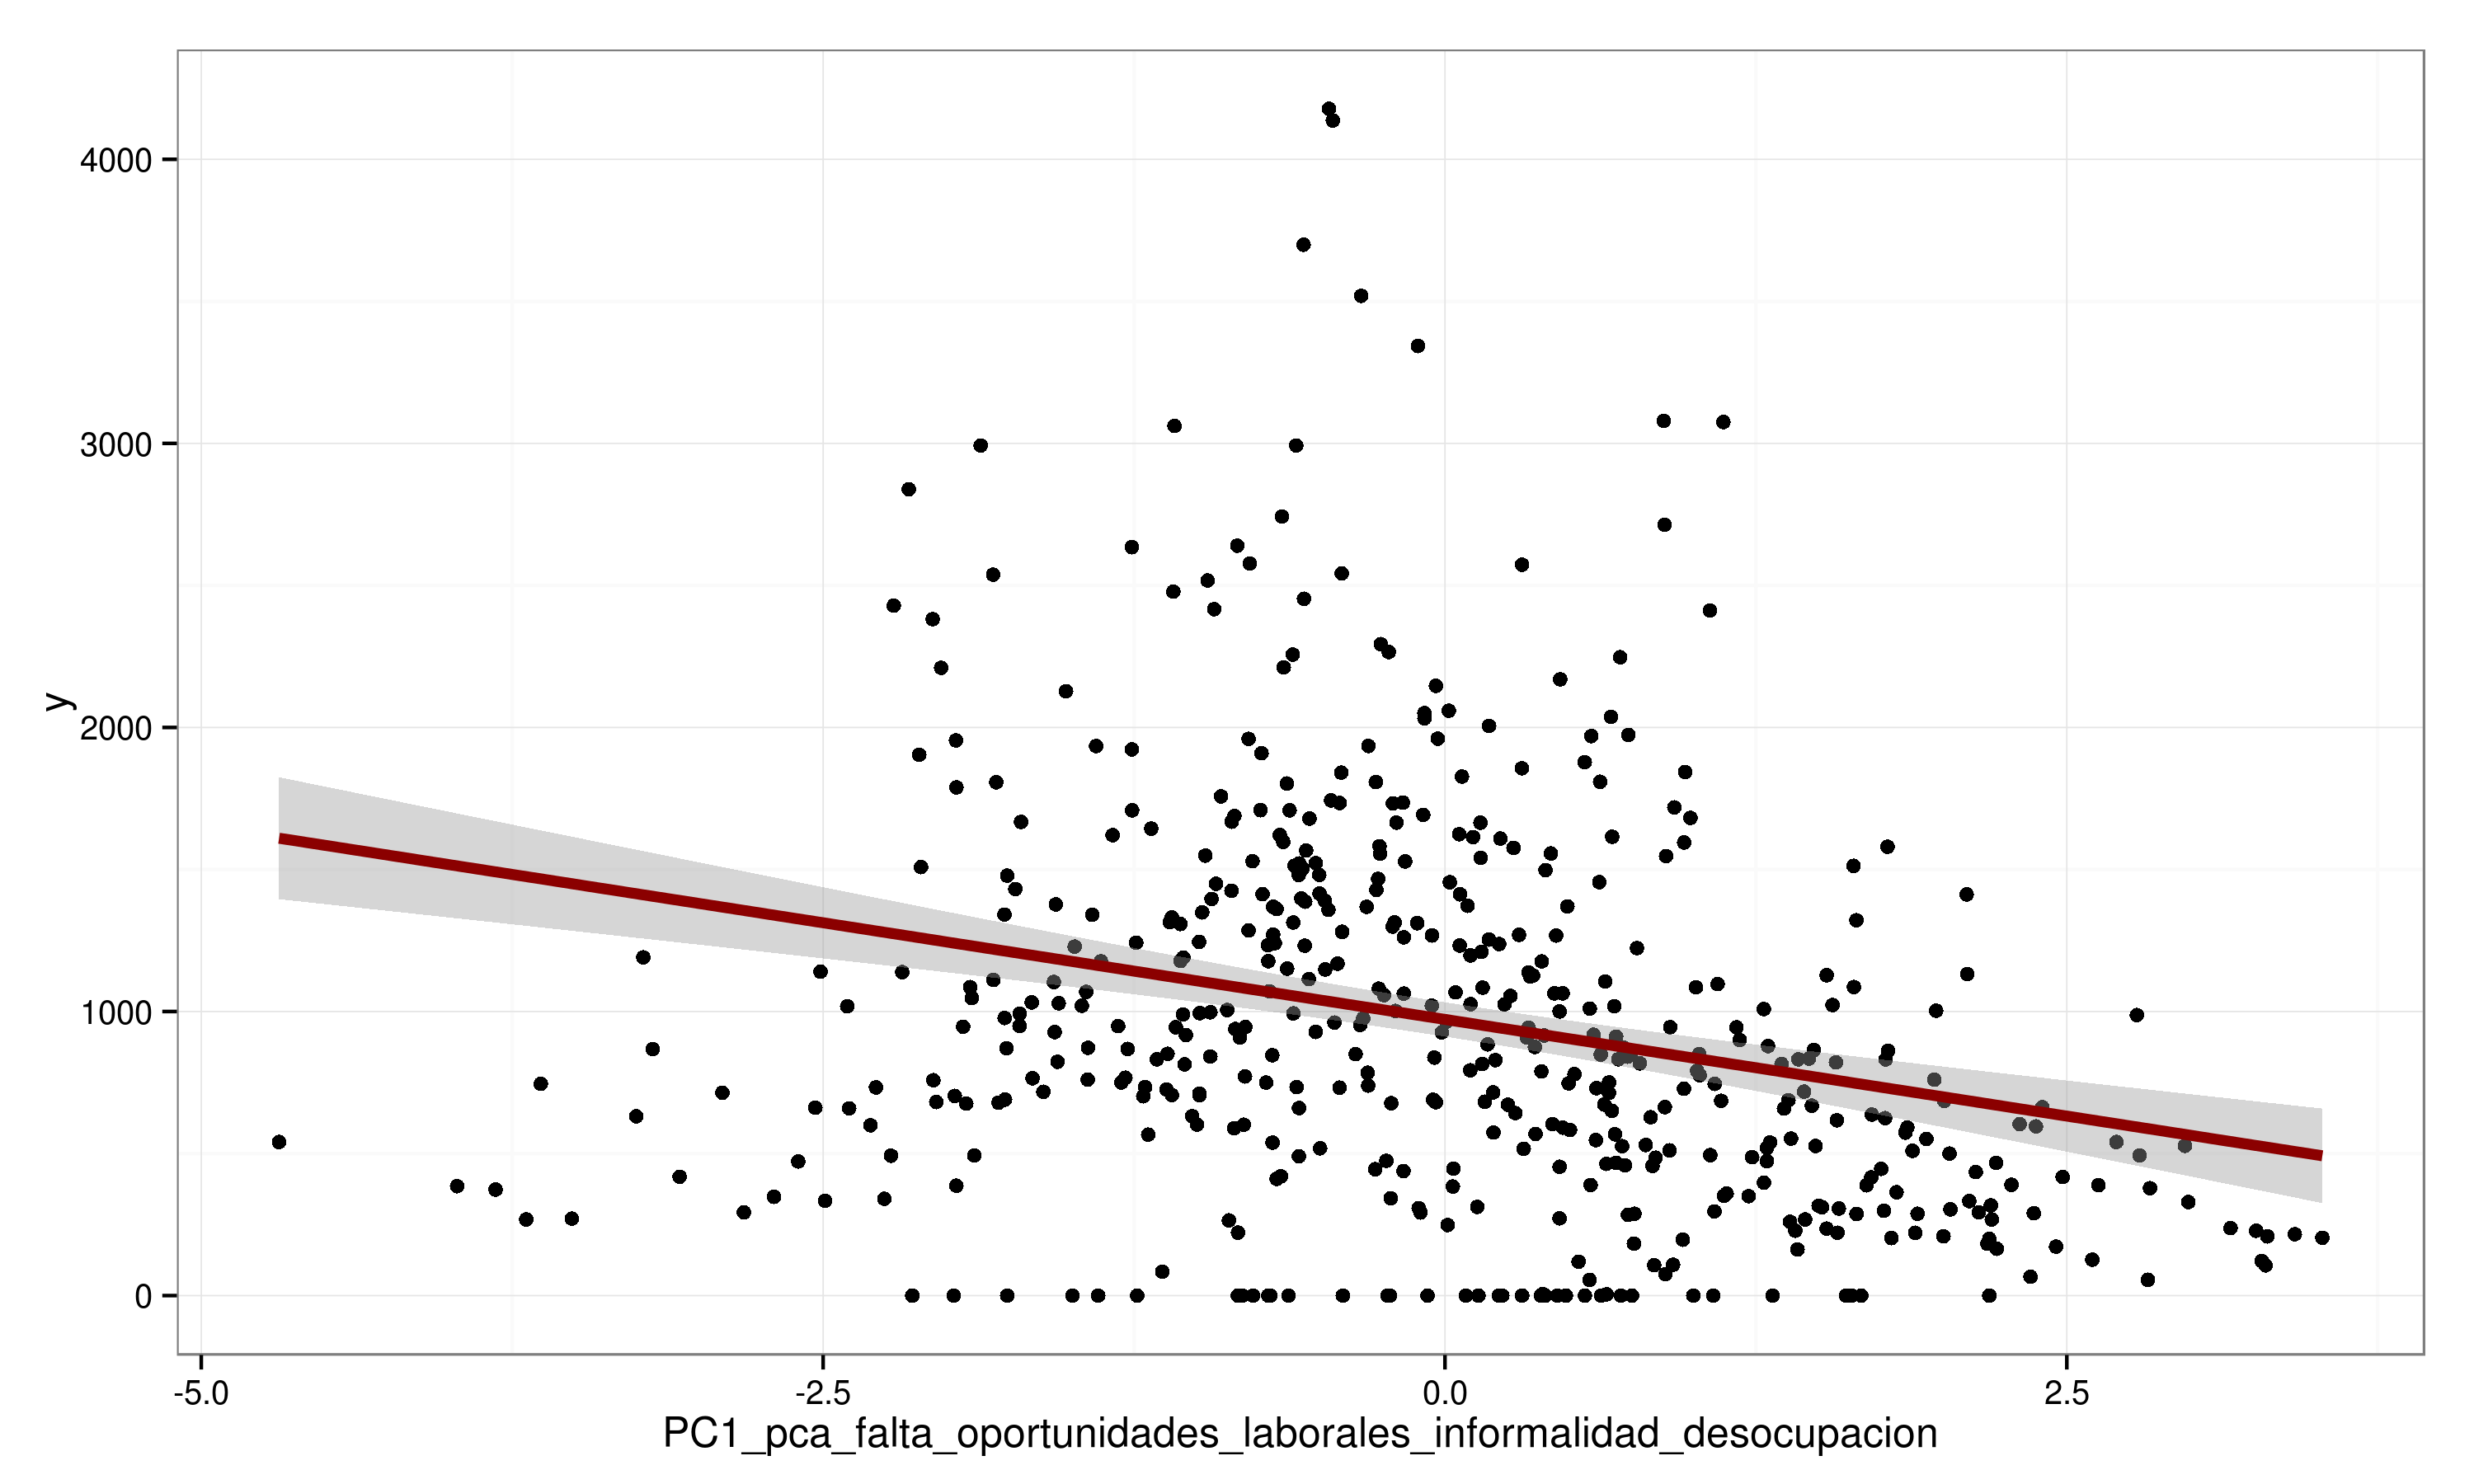
\includegraphics{img/y_indep17.png}

\end{frame}

\begin{frame}{Factores de riesgo}

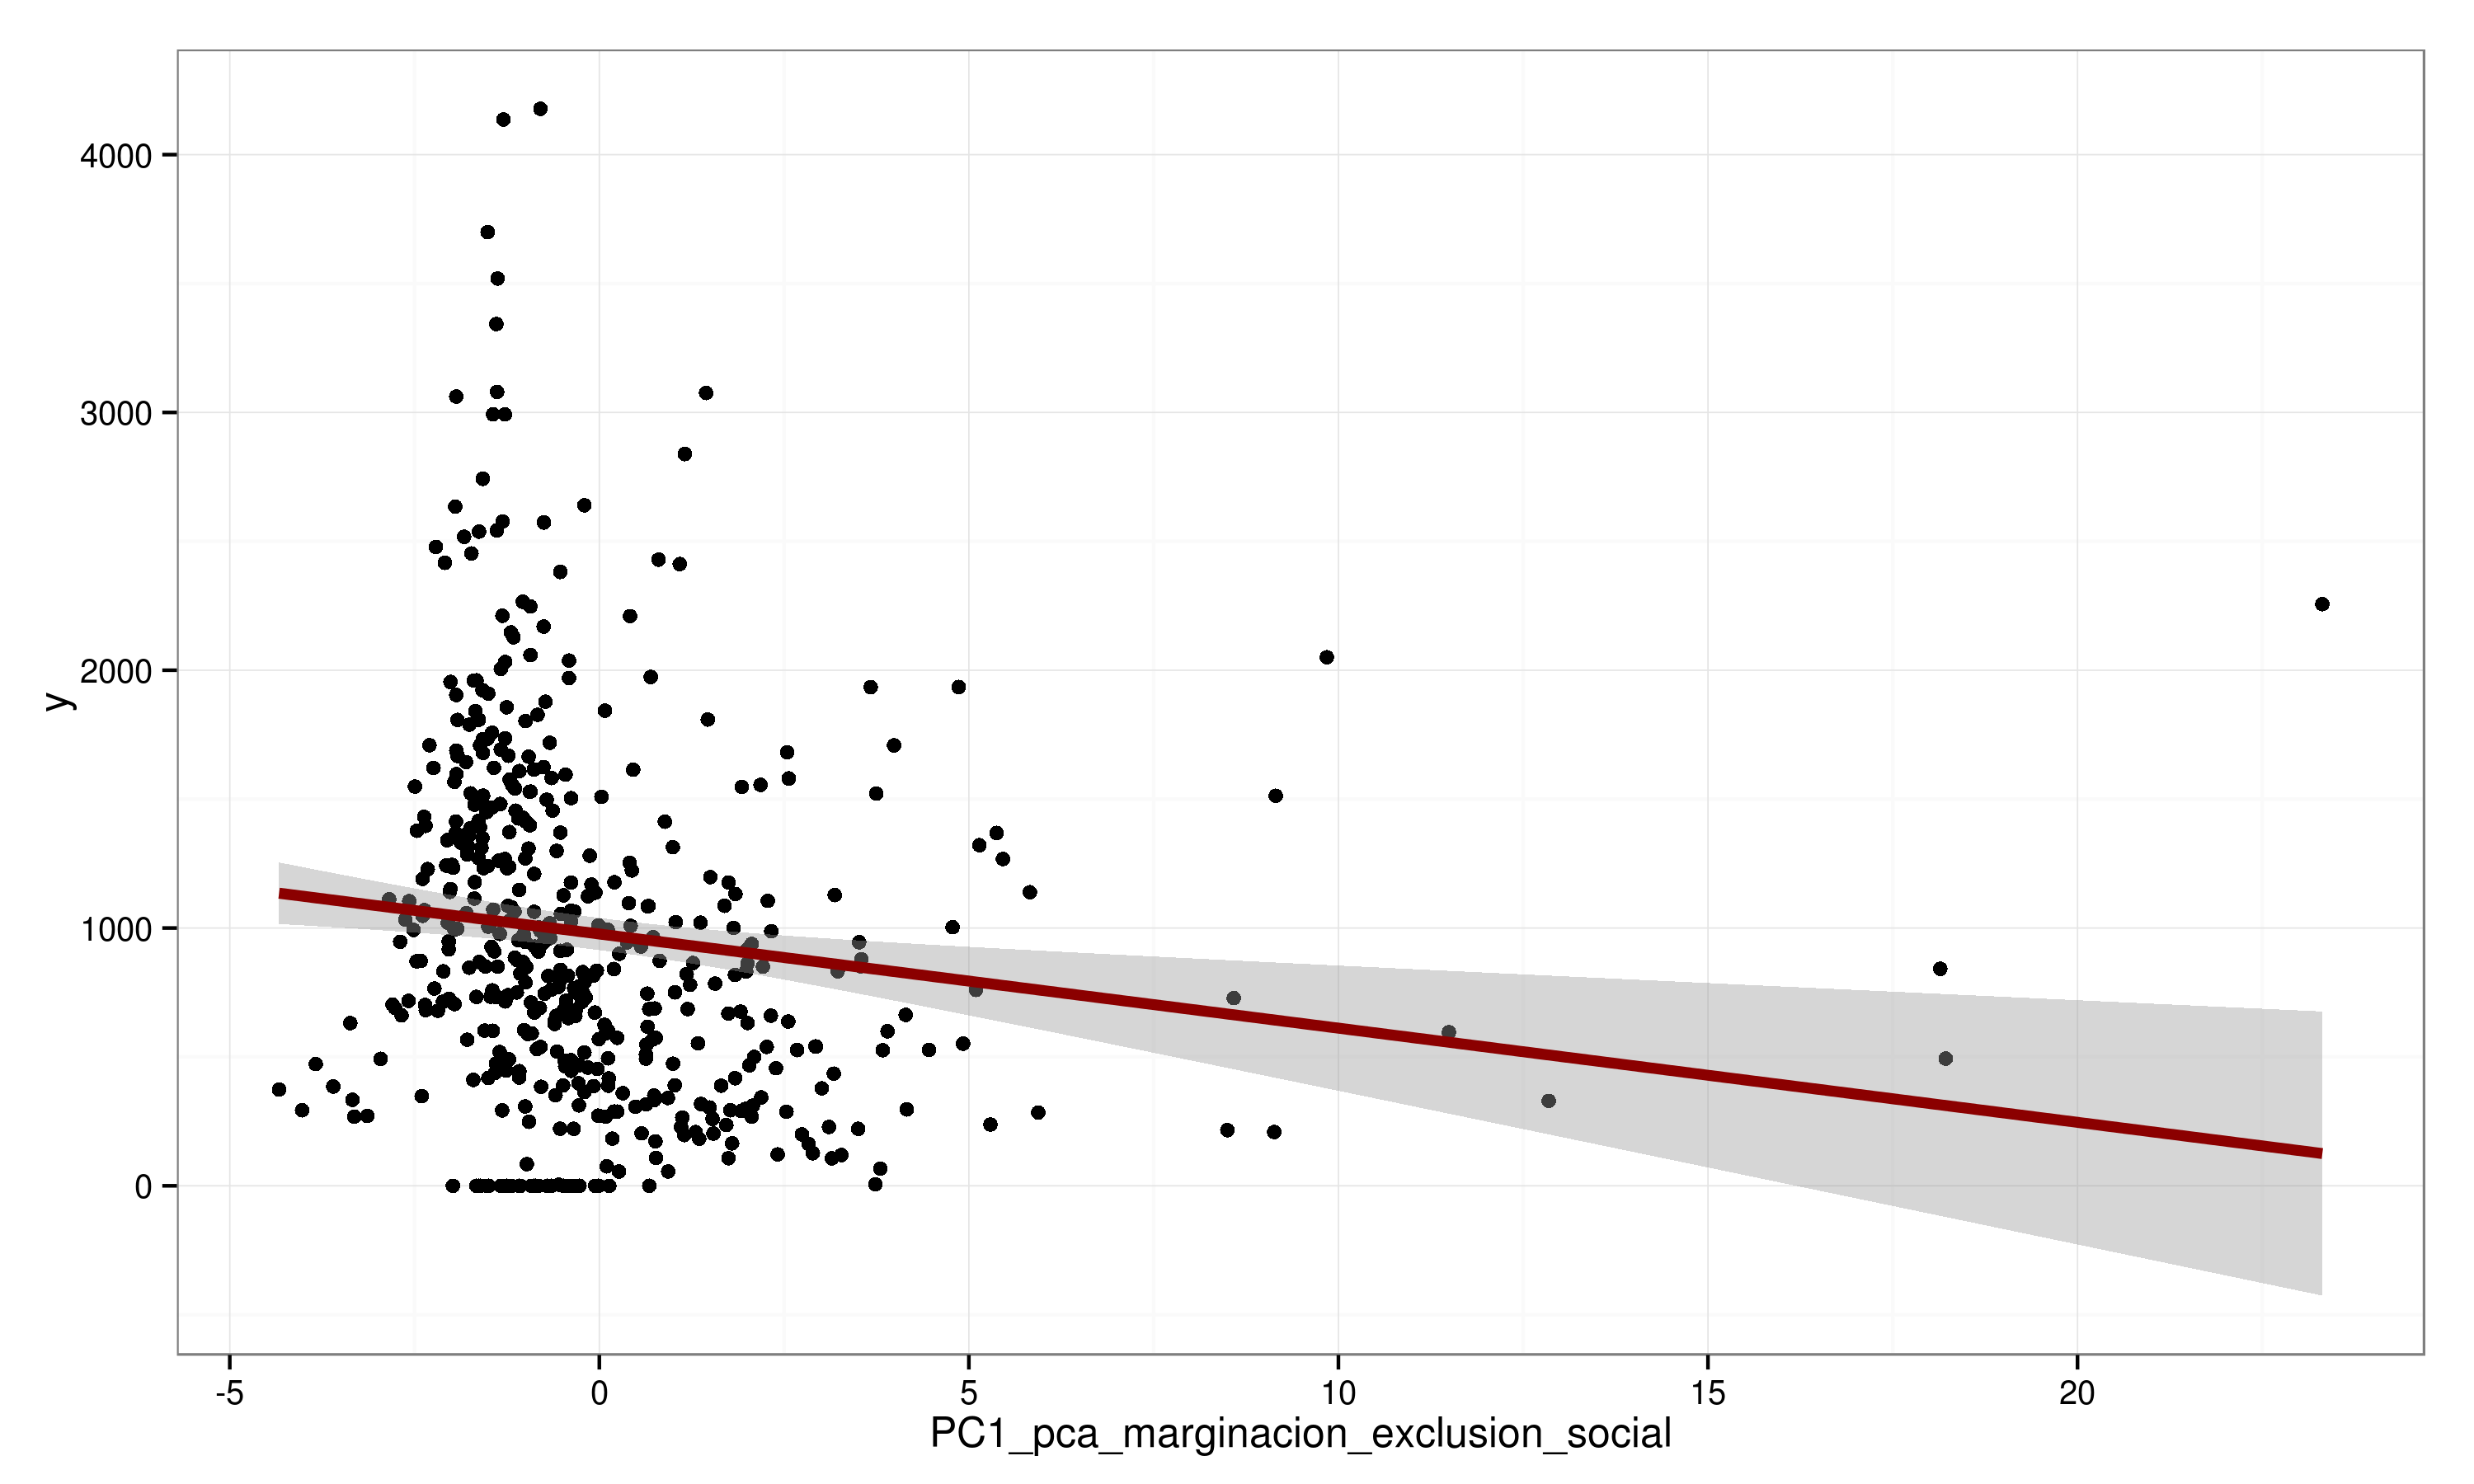
\includegraphics{img/y_indep18.png}

\end{frame}

\begin{frame}{Factores de riesgo}

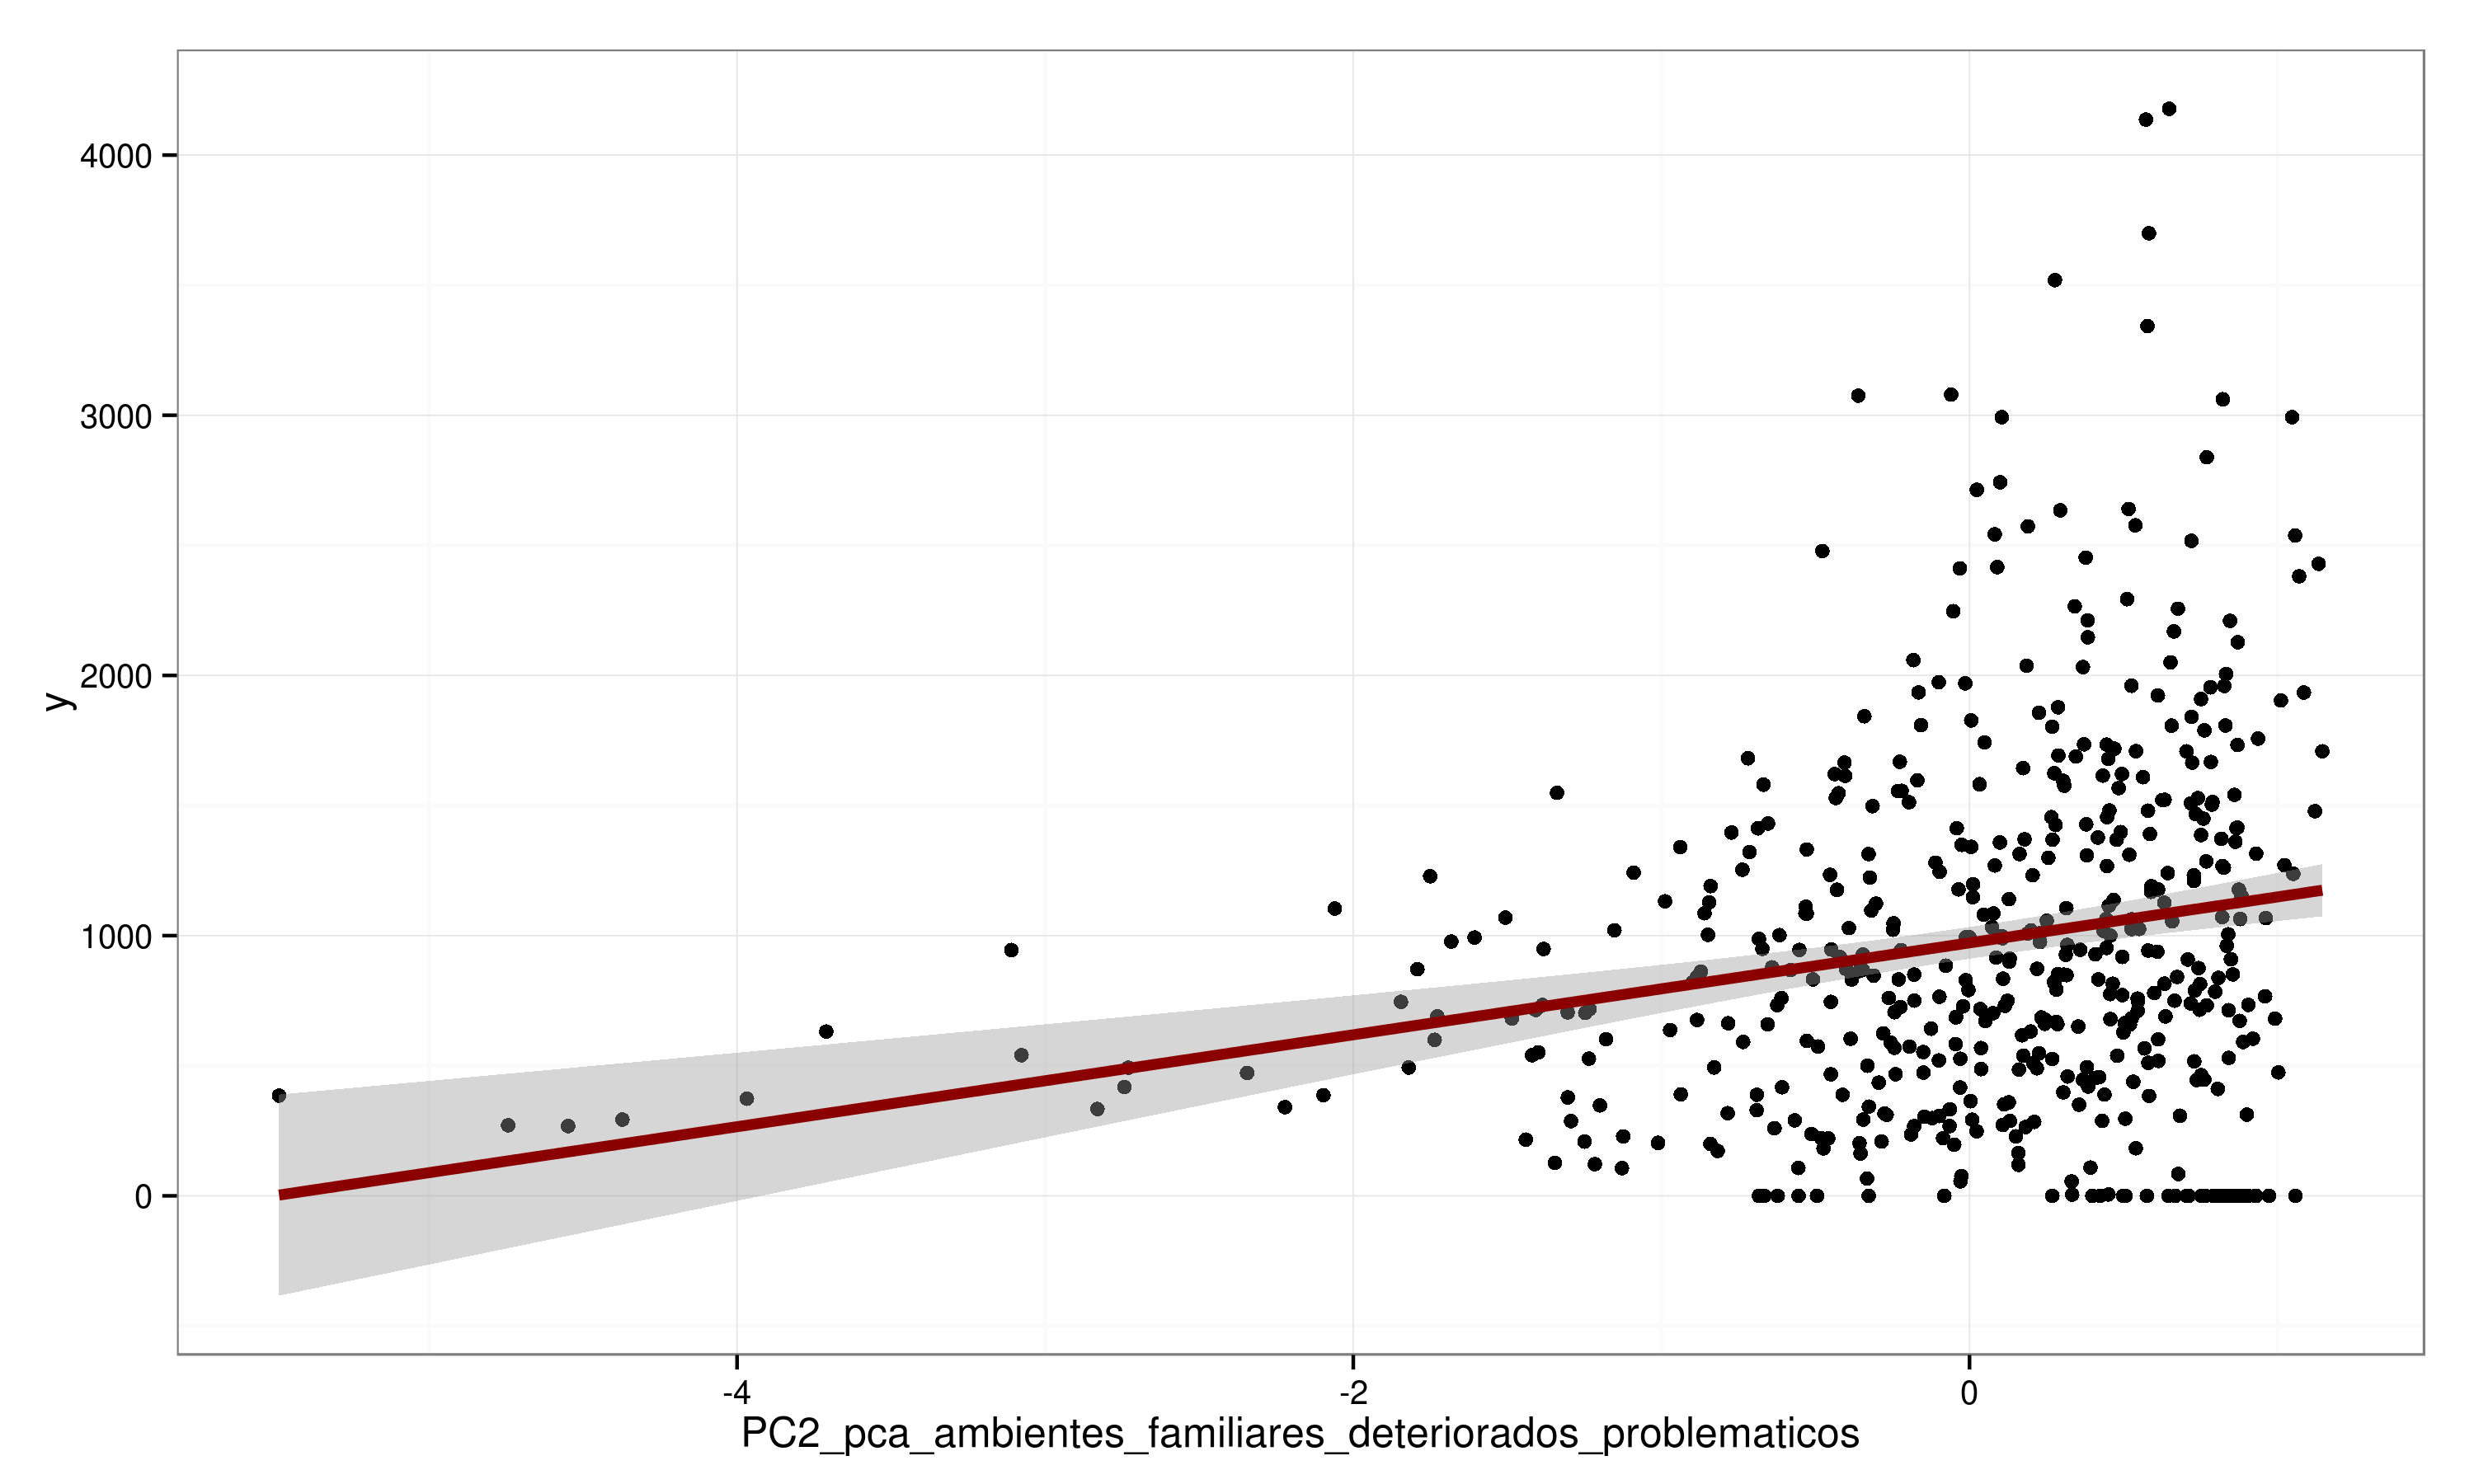
\includegraphics{img/y_indep19.png}

\end{frame}

\begin{frame}{Factores de riesgo}

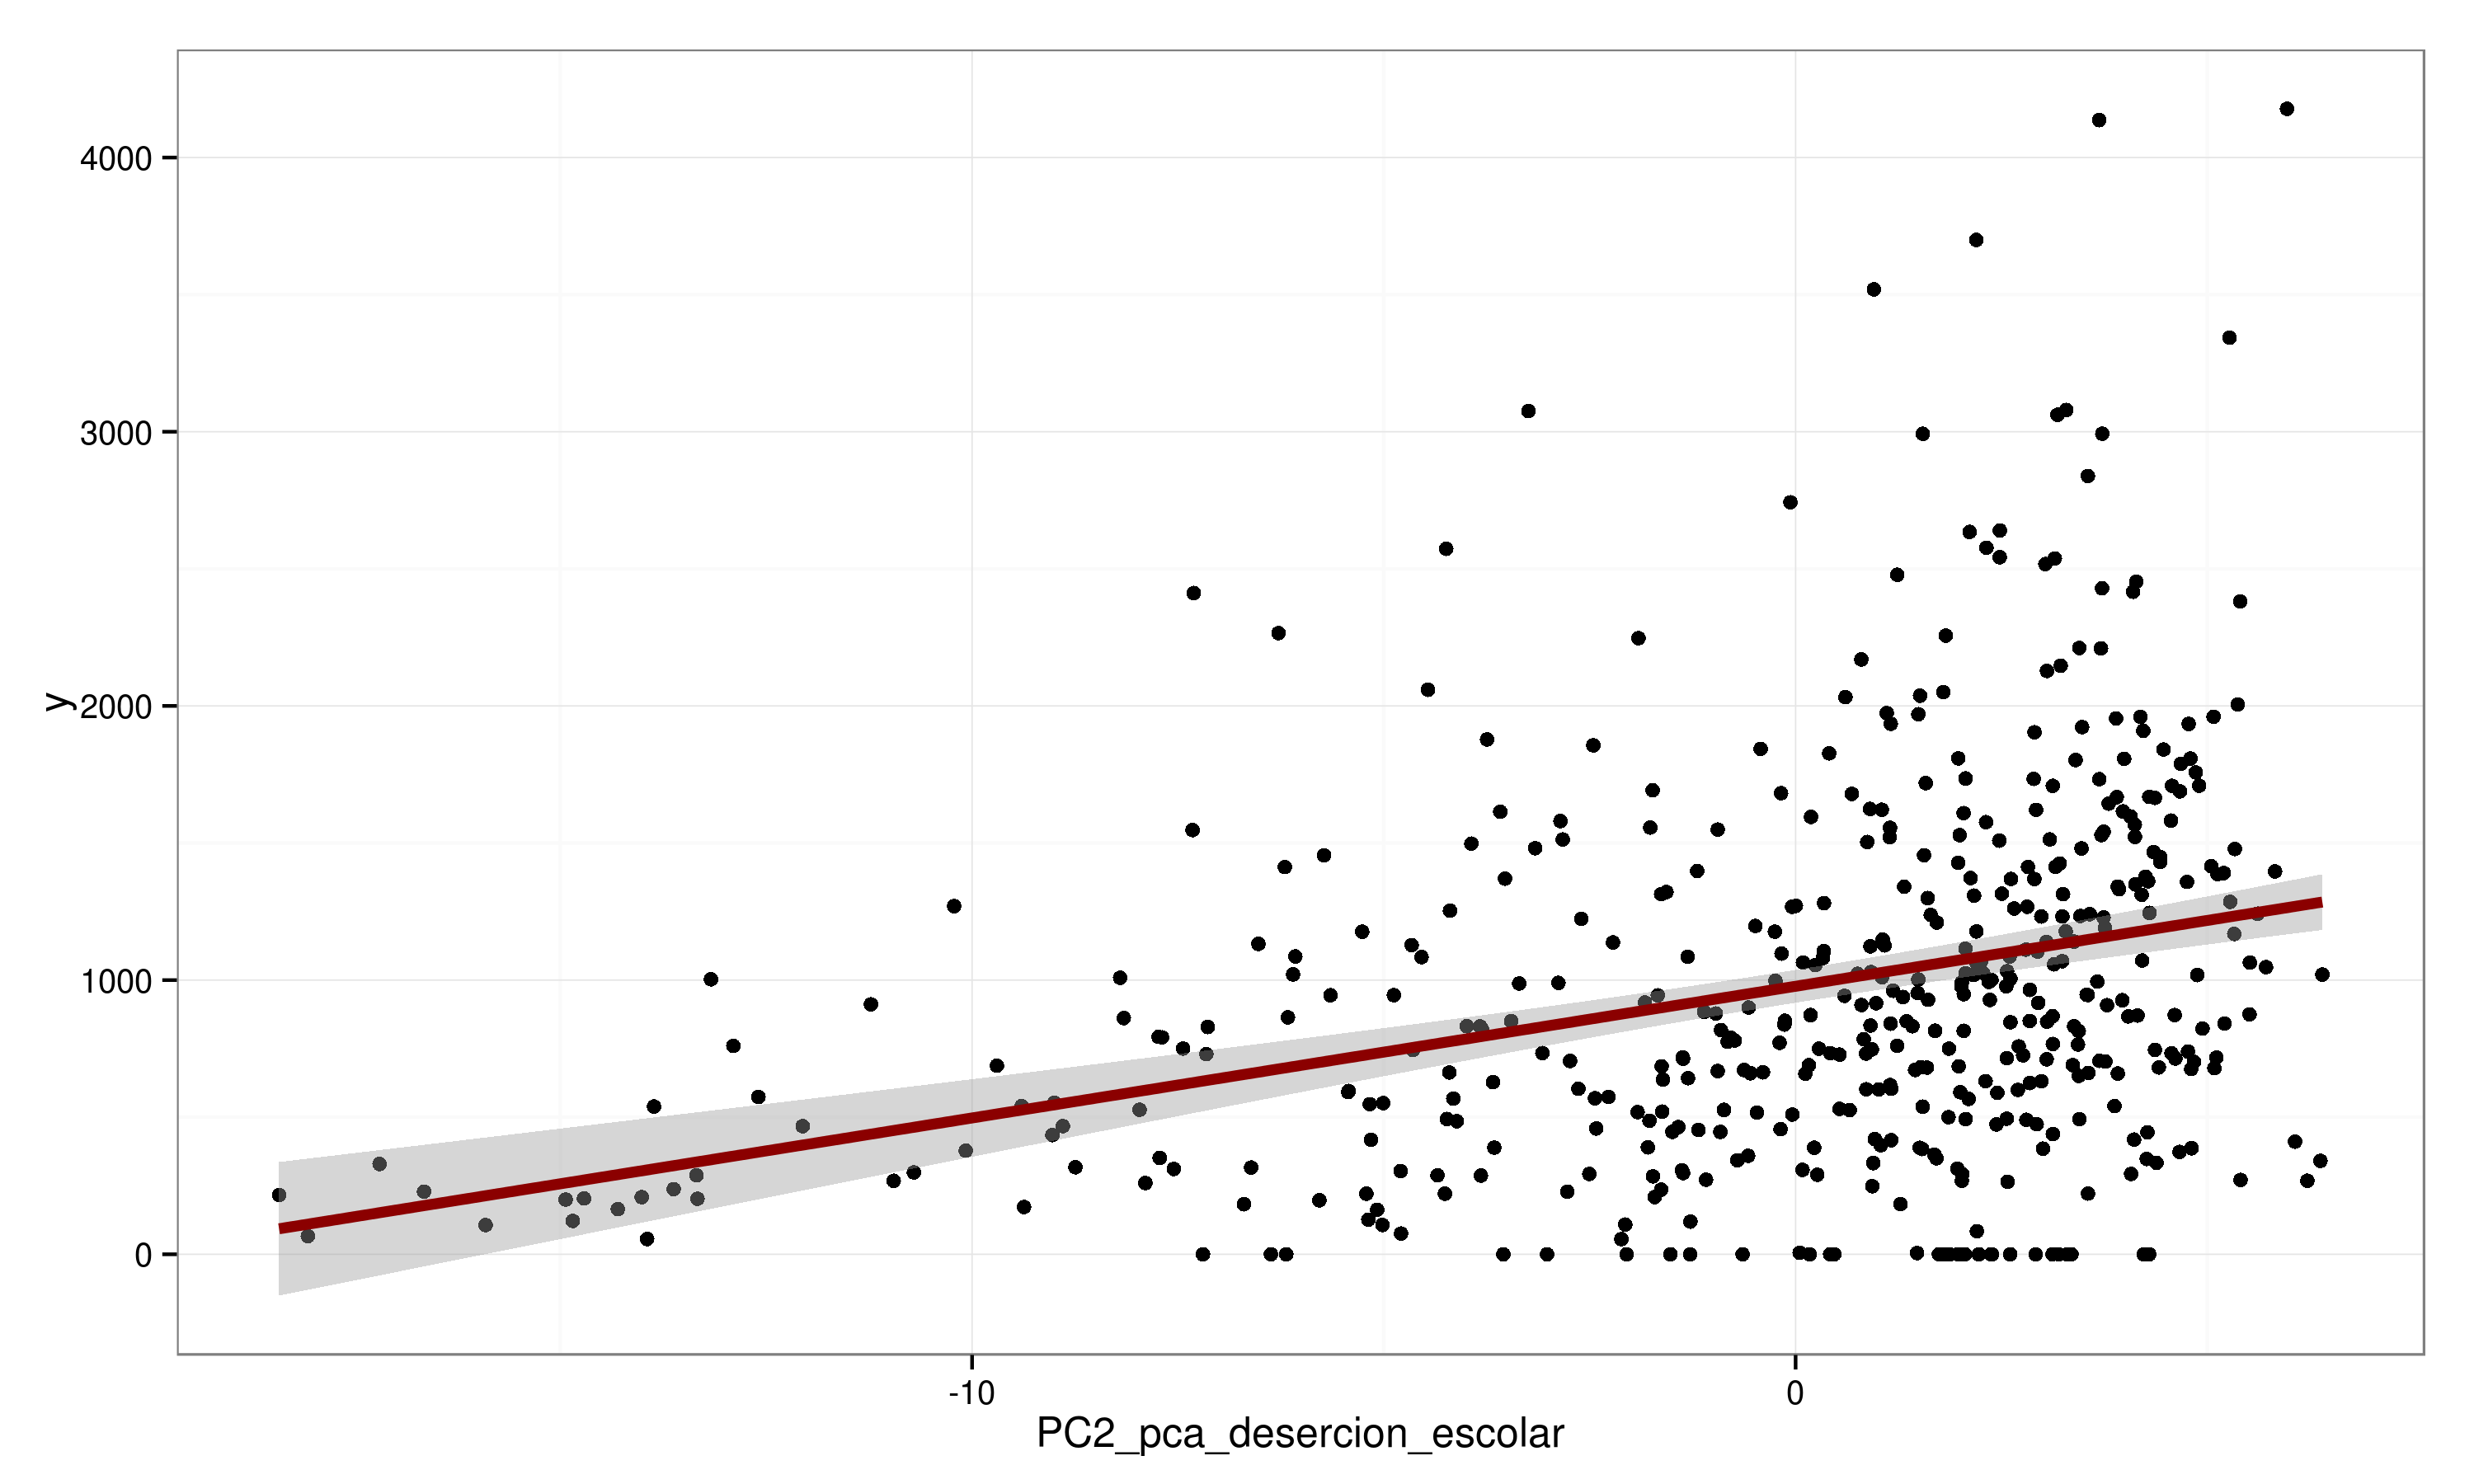
\includegraphics{img/y_indep22.png}

\end{frame}

\begin{frame}{Factores de riesgo}

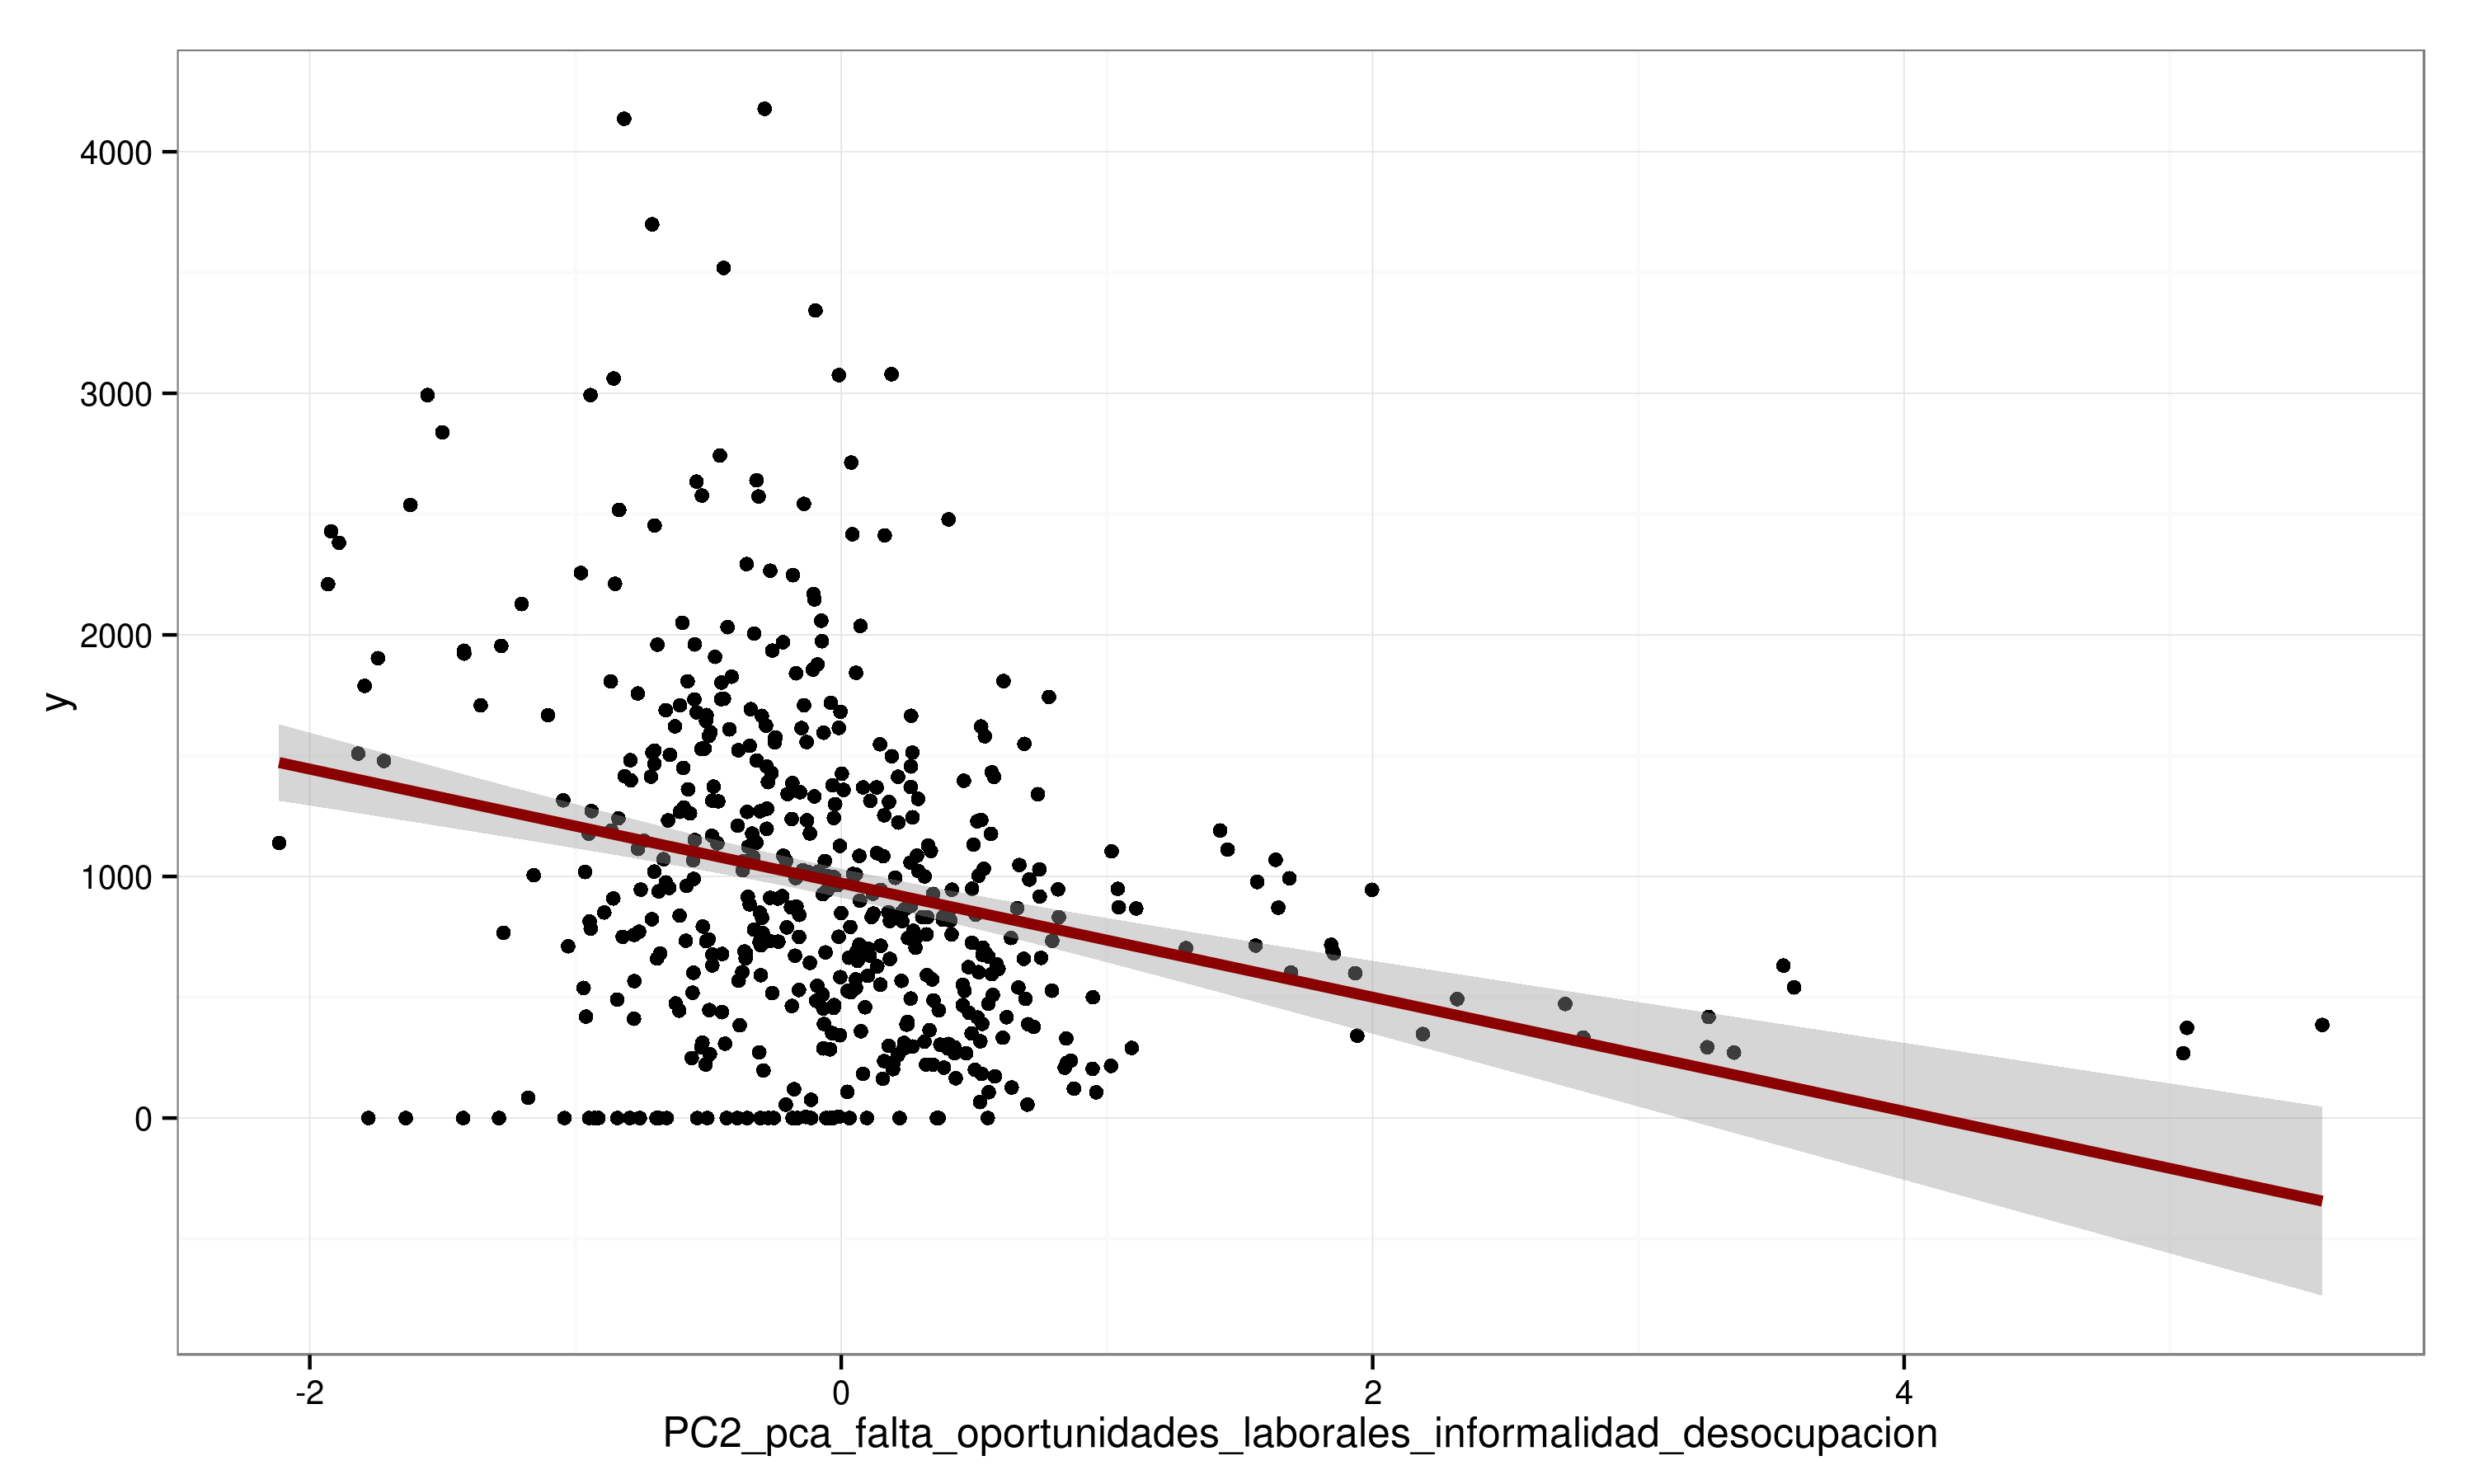
\includegraphics{img/y_indep25.png}

\end{frame}

\begin{frame}{Factores de riesgo}

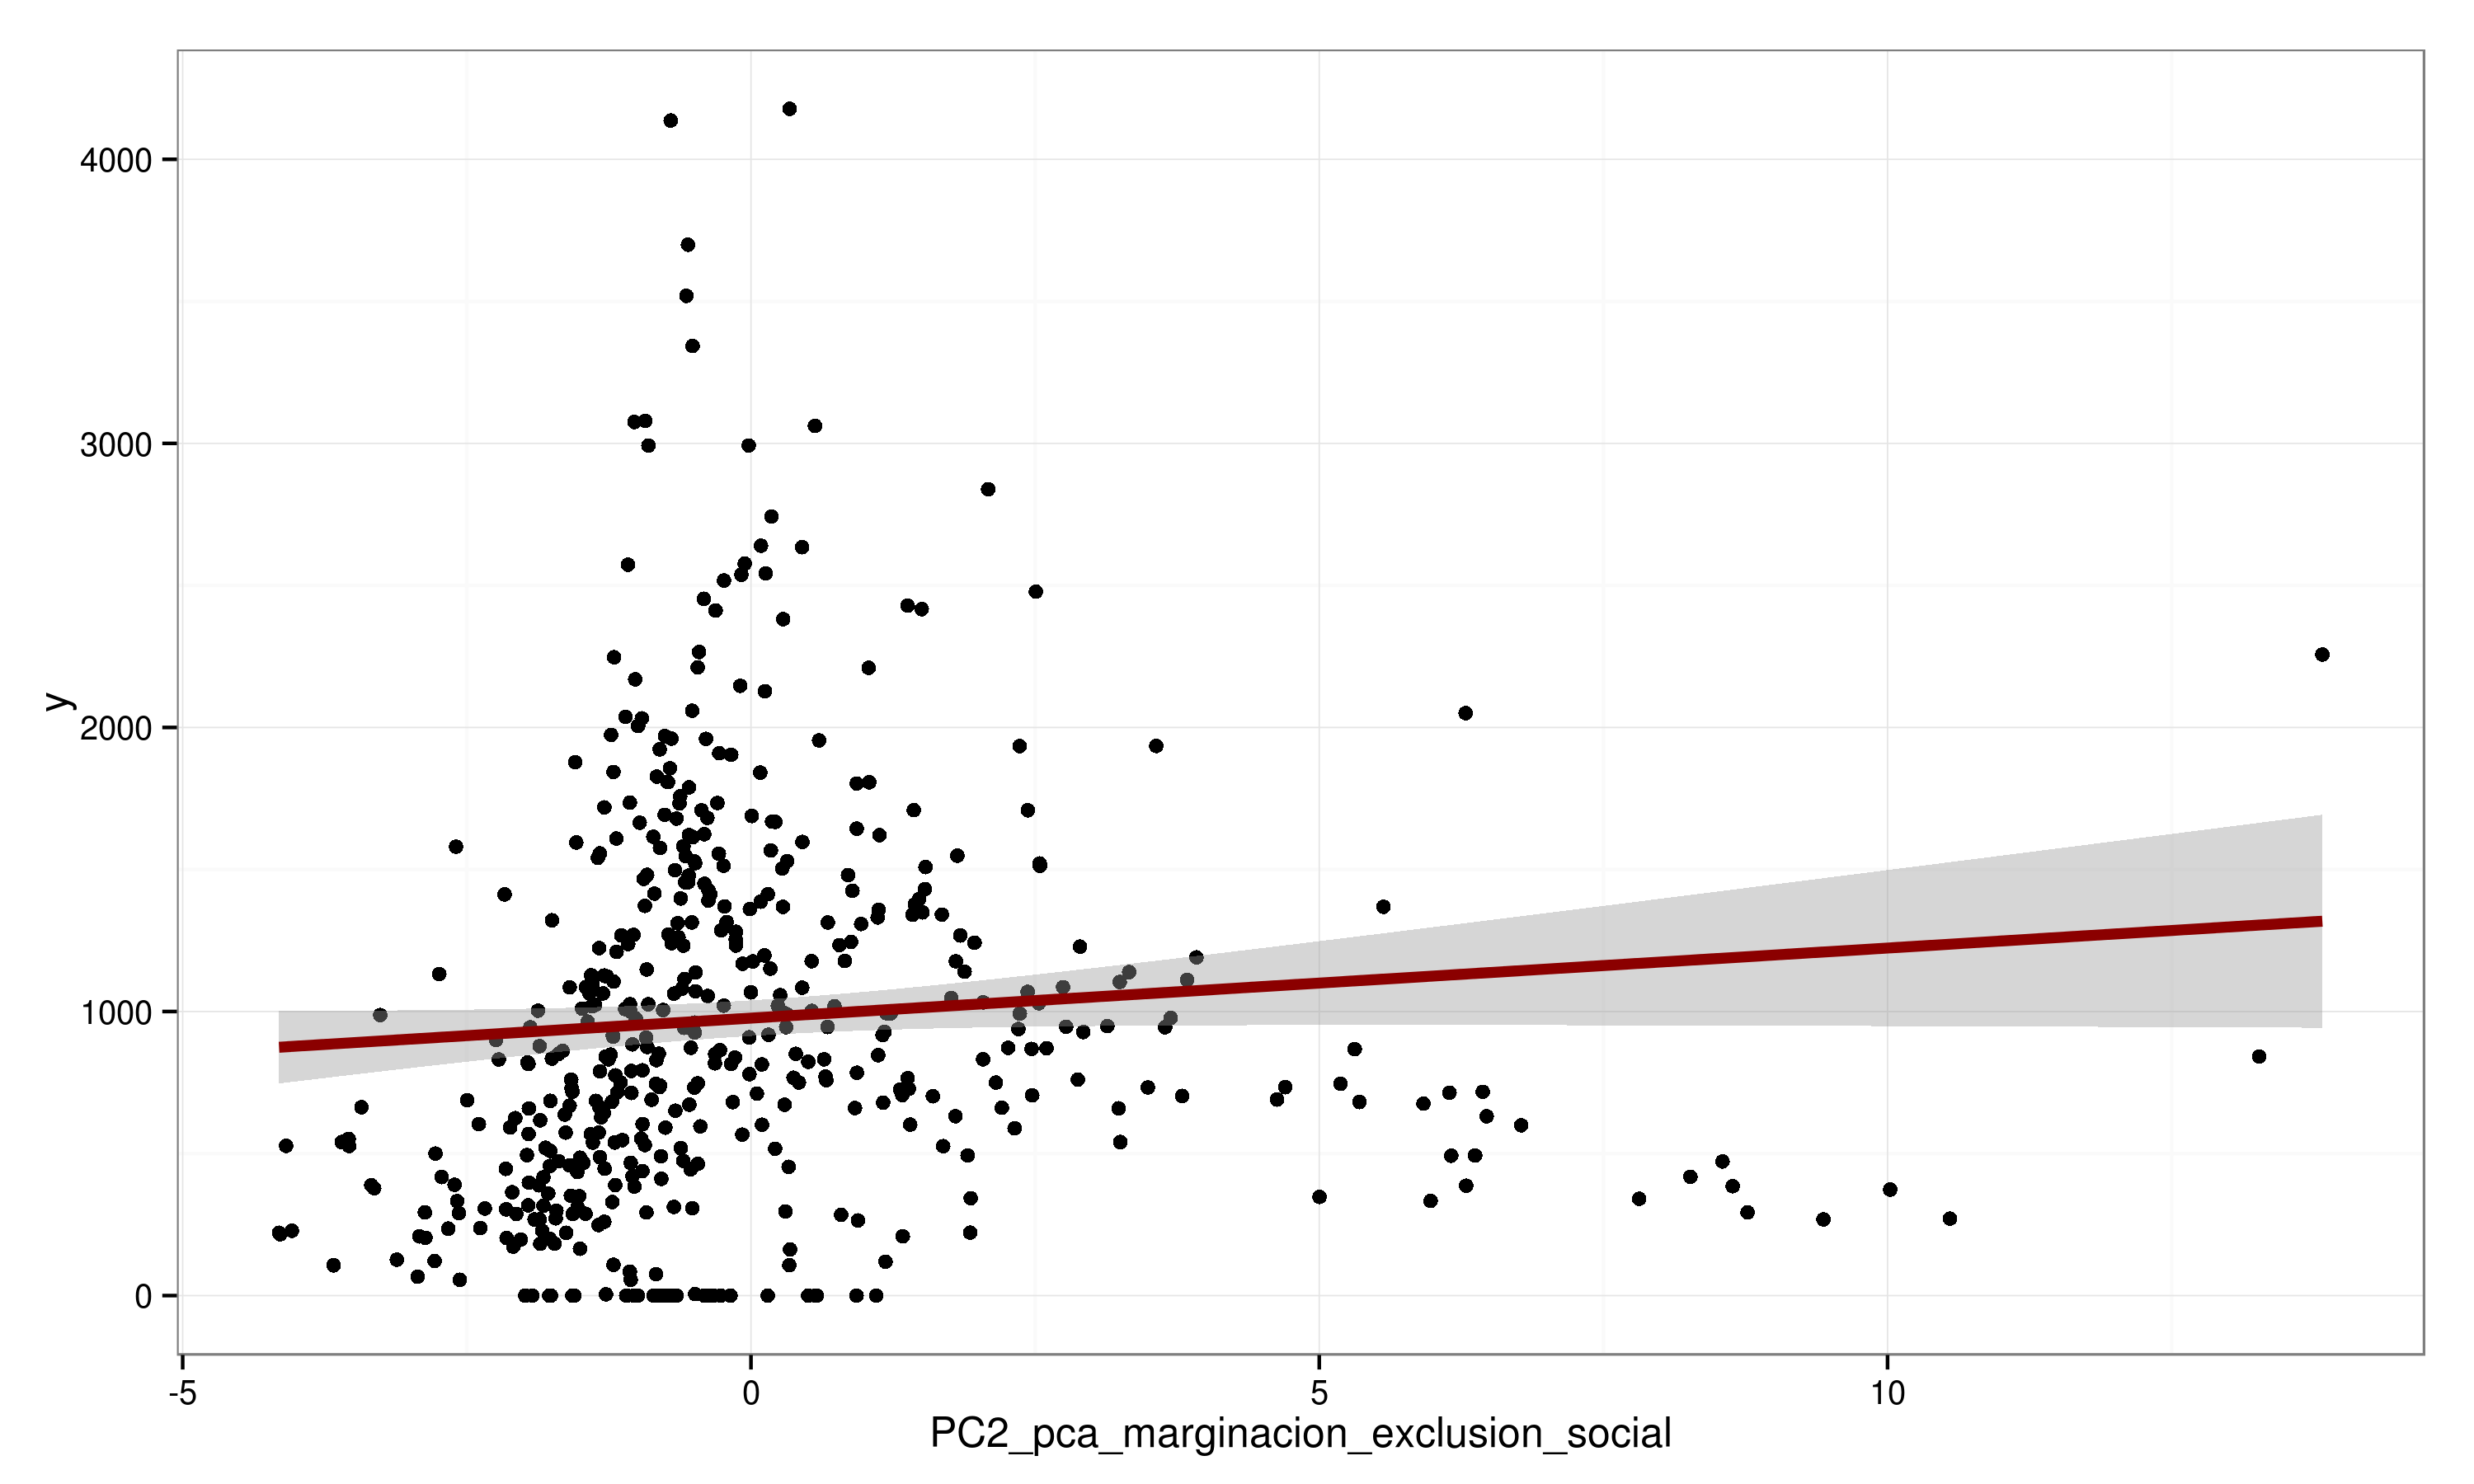
\includegraphics{img/y_indep26.png}

\end{frame}

\begin{frame}{Factores de riesgo}

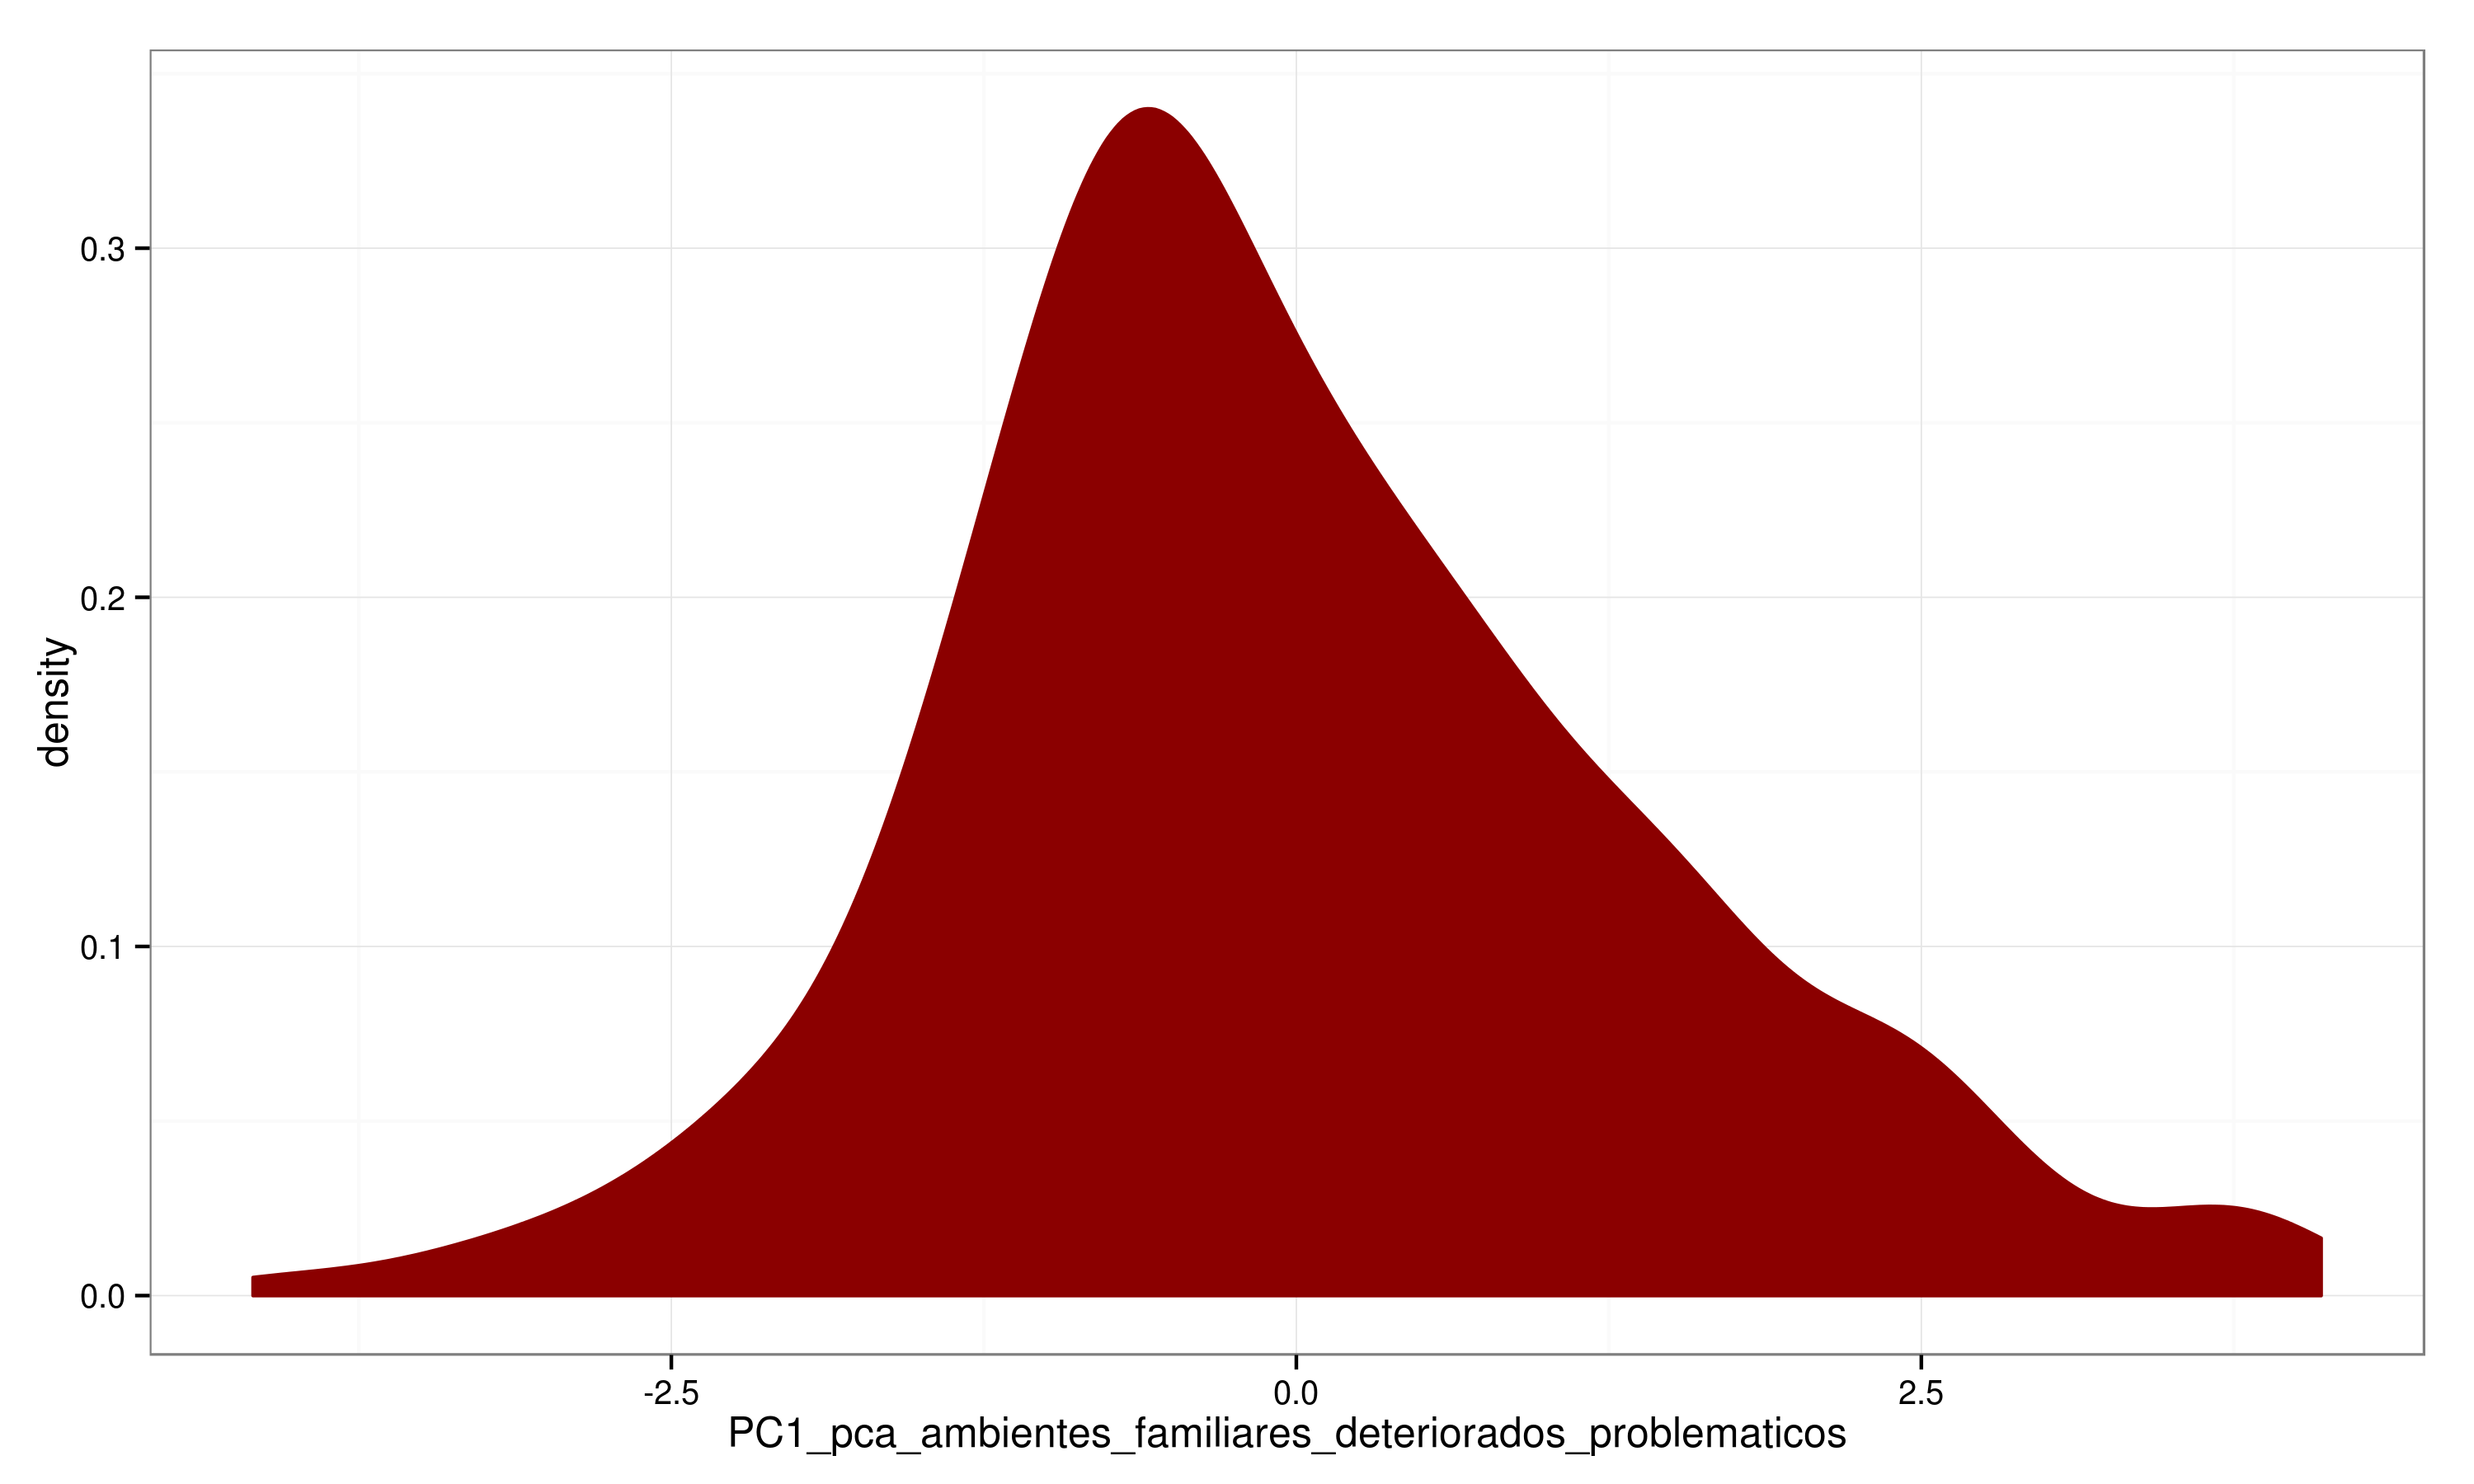
\includegraphics{img/x_density11.png}

\end{frame}

\begin{frame}{Factores de riesgo}

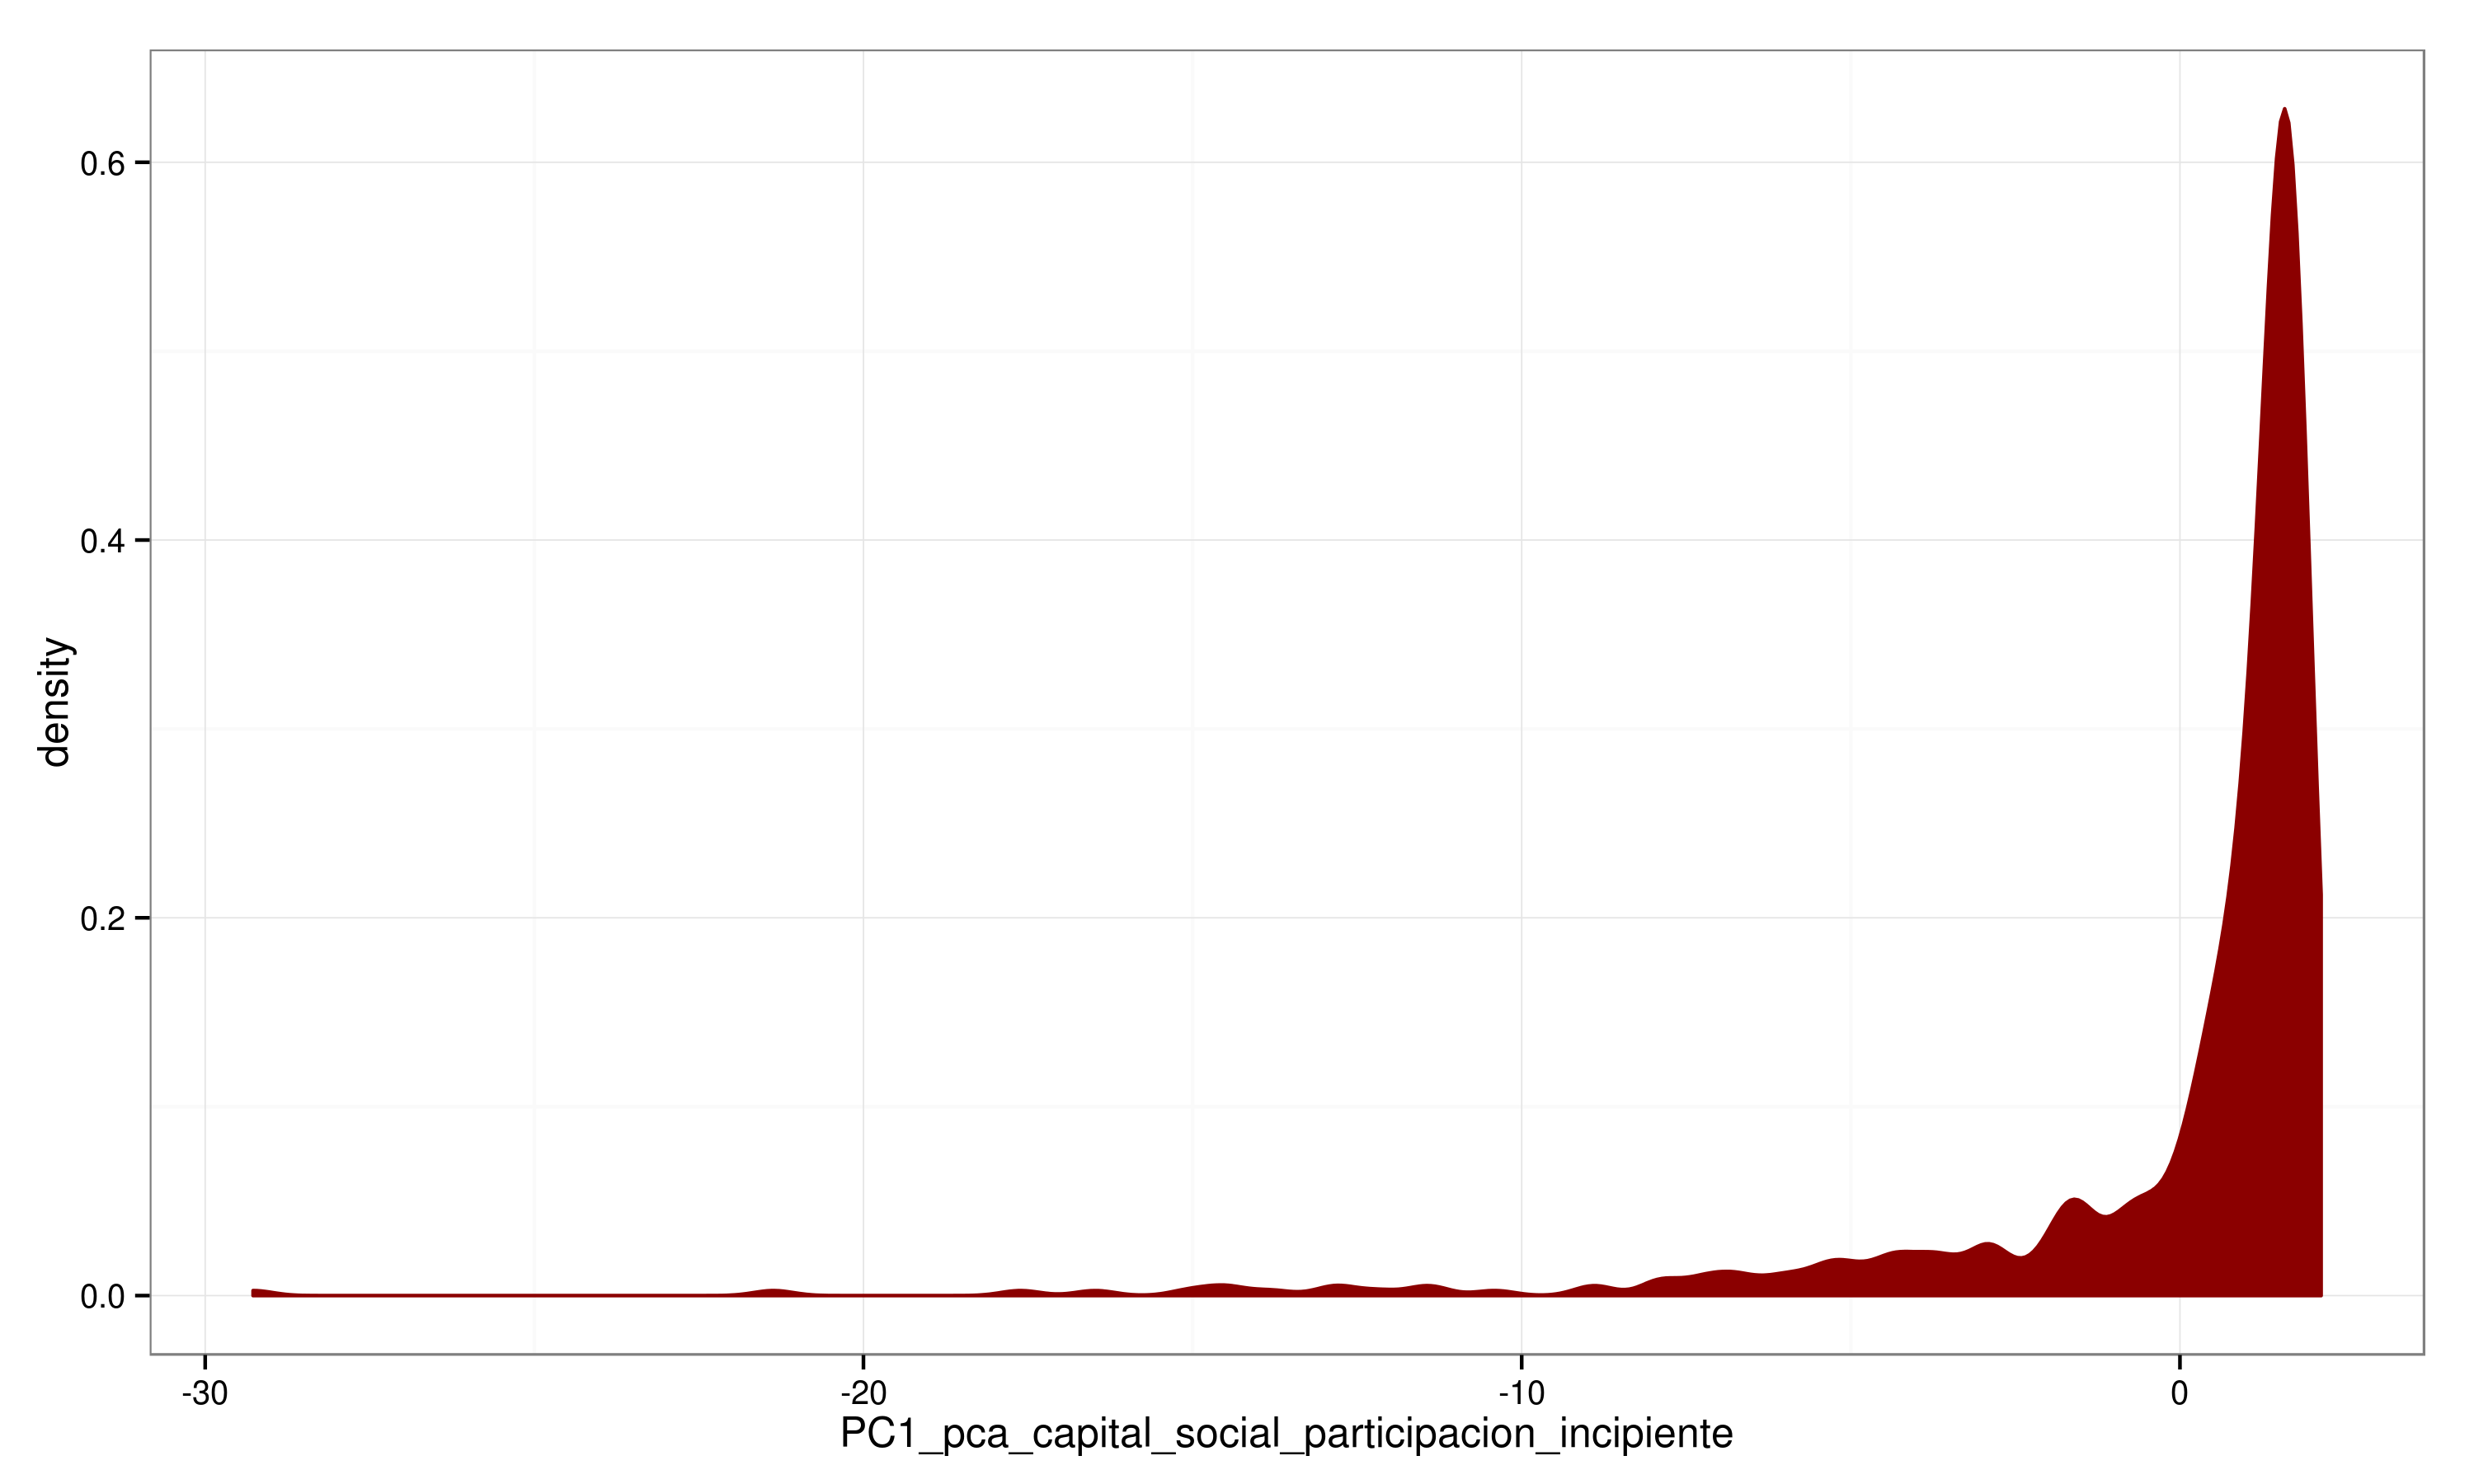
\includegraphics{img/x_density12.png}

\end{frame}

\begin{frame}{Factores de riesgo}

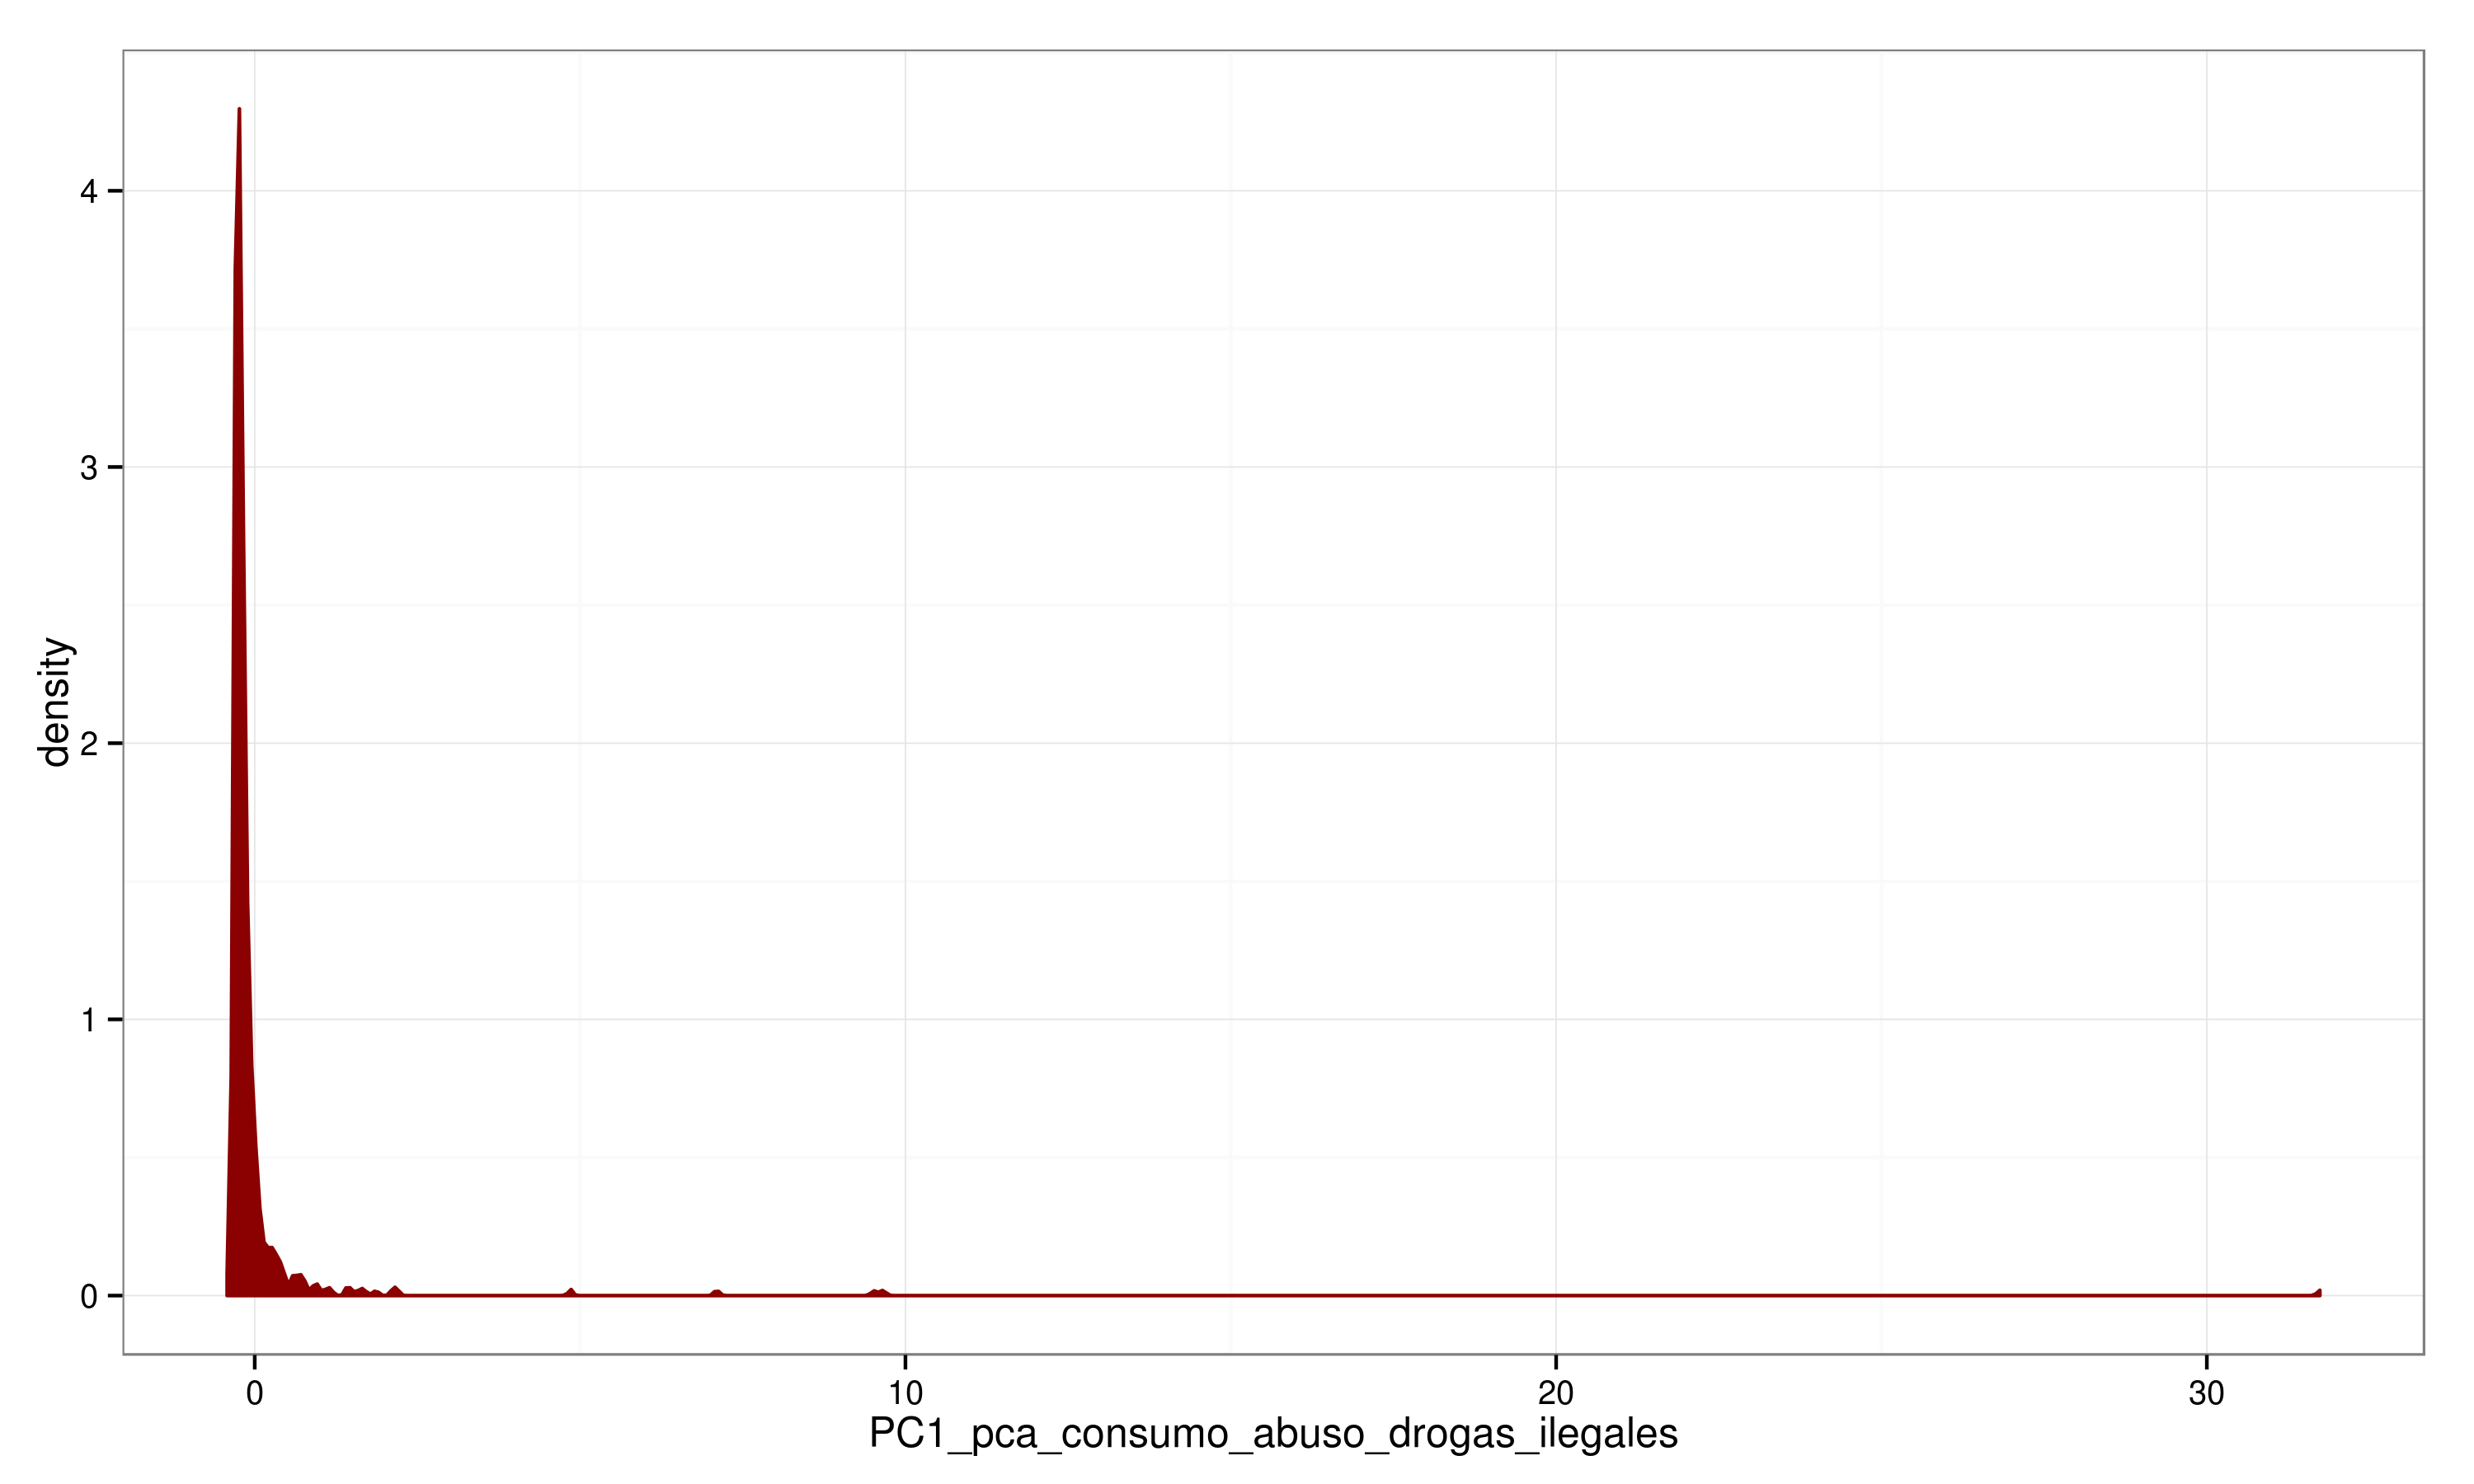
\includegraphics{img/x_density13.png}

\end{frame}

\begin{frame}{Factores de riesgo}

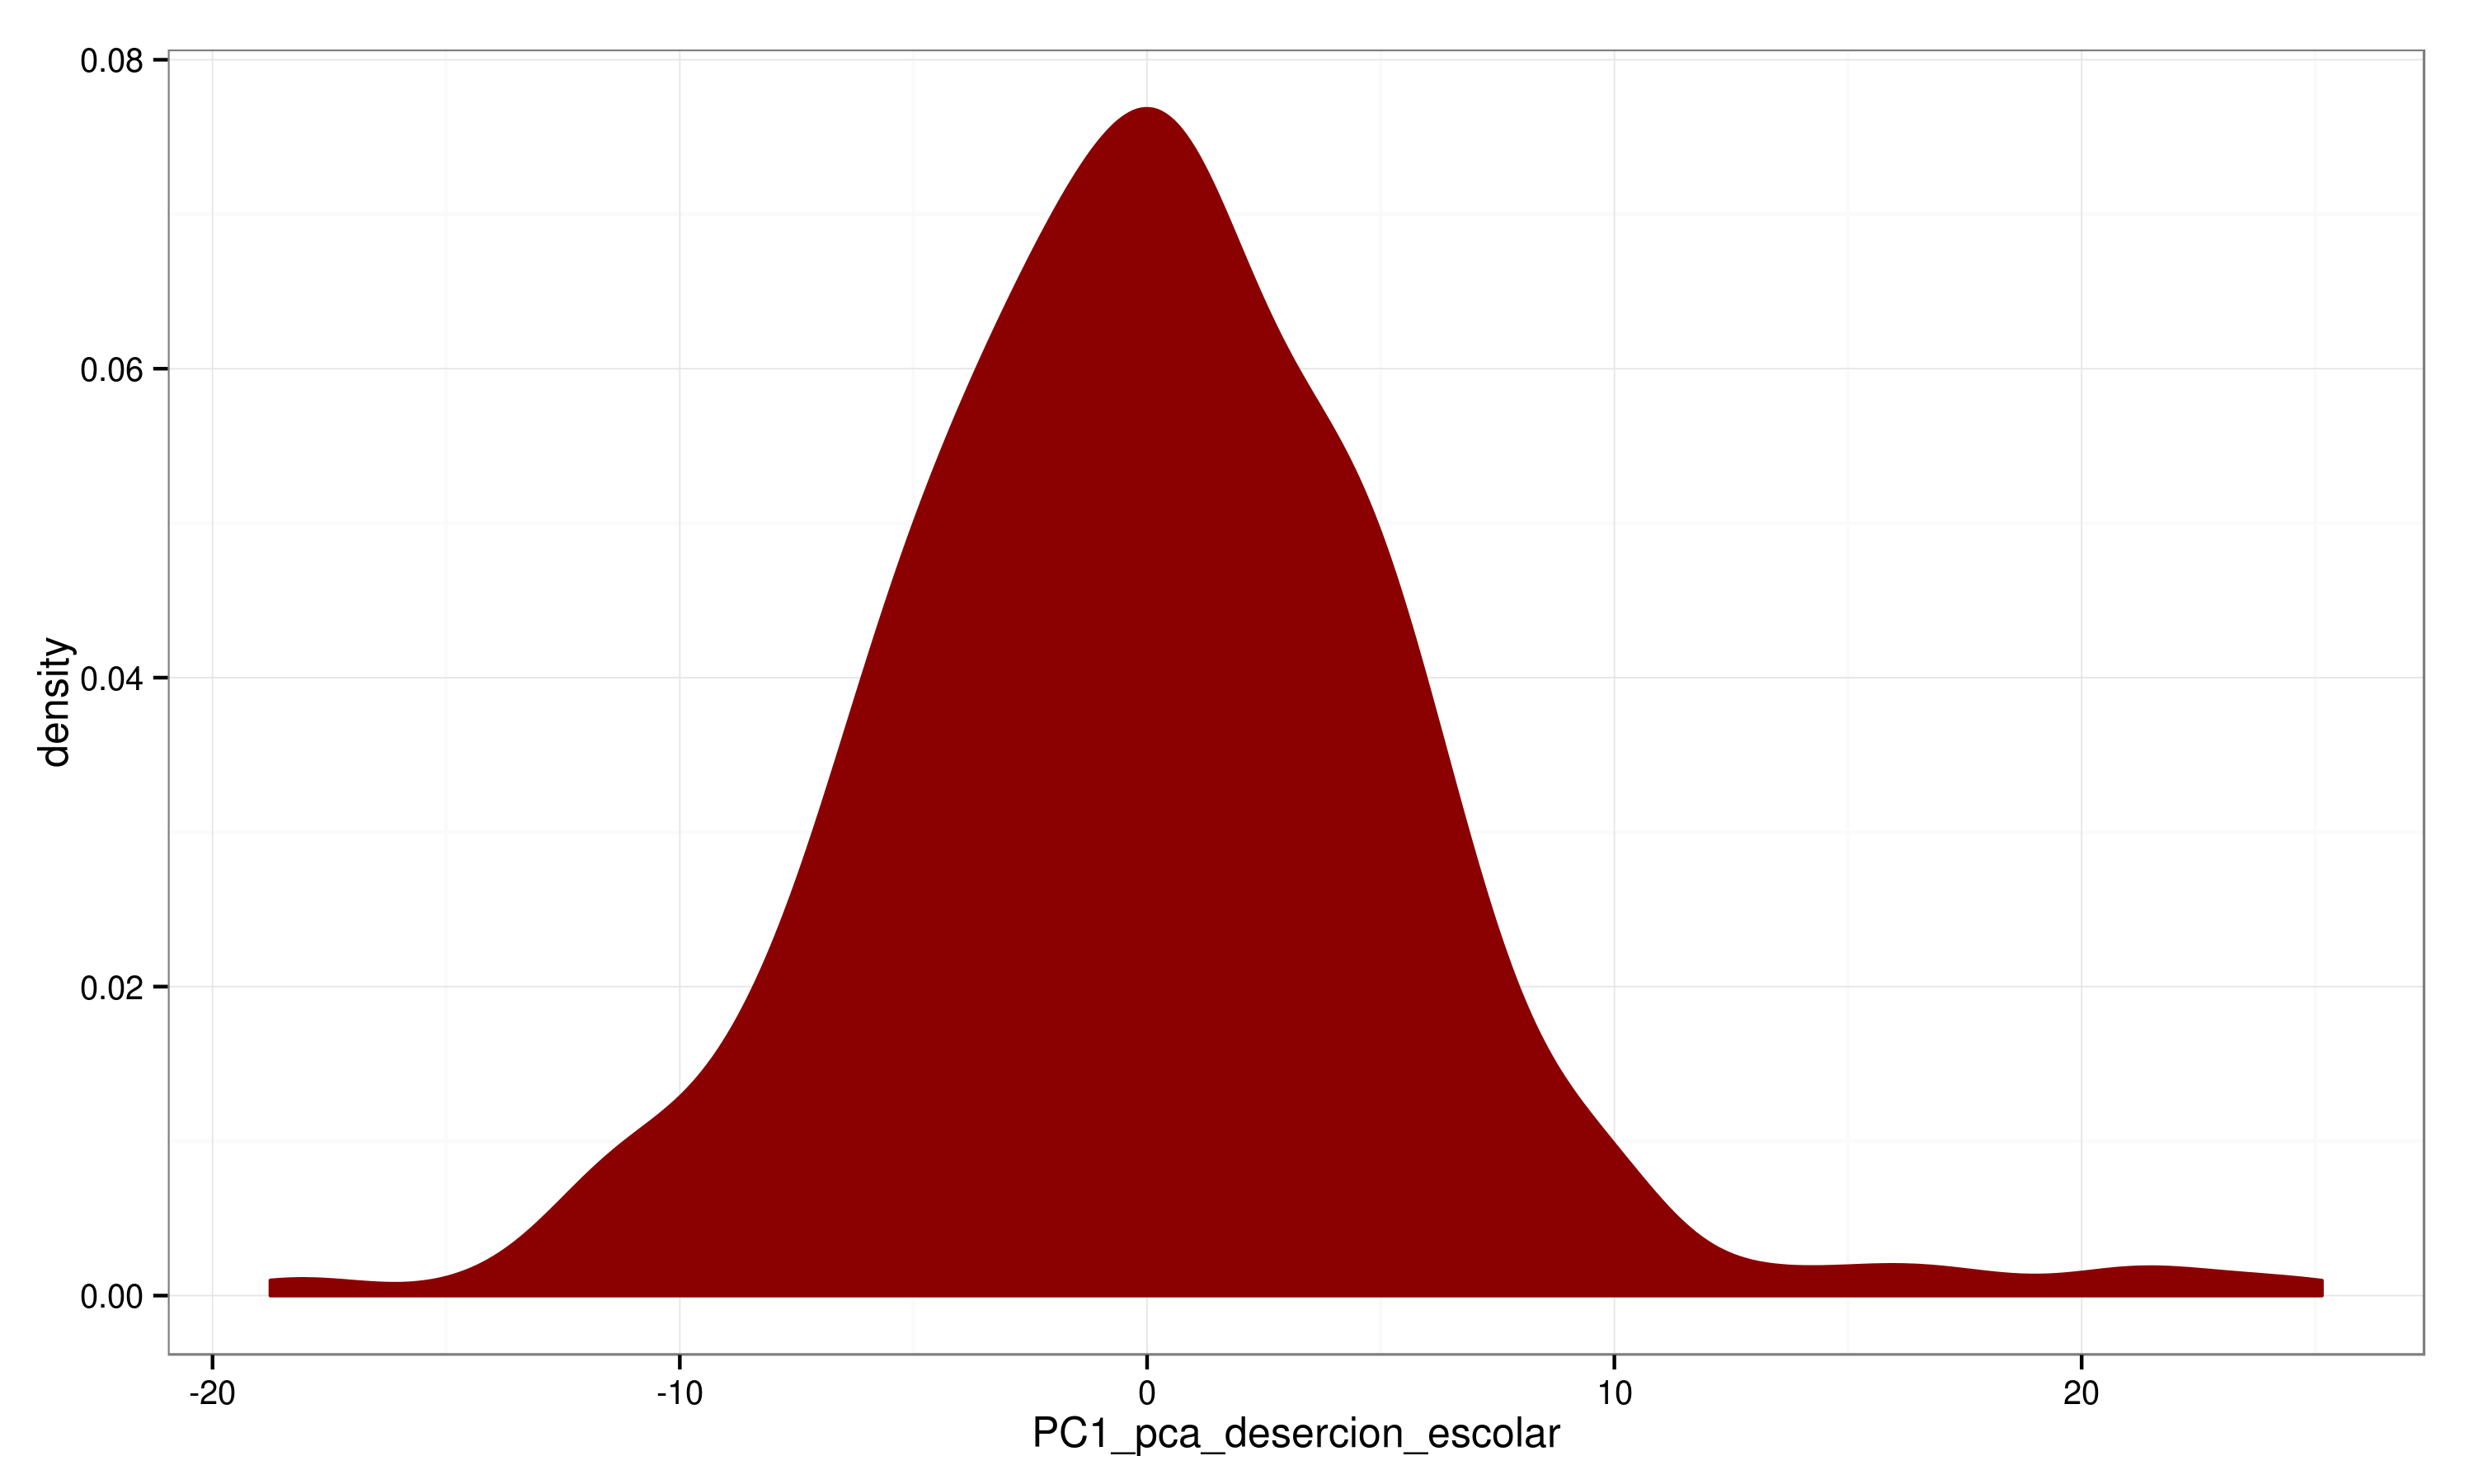
\includegraphics{img/x_density14.png}

\end{frame}

\begin{frame}{Factores de riesgo}

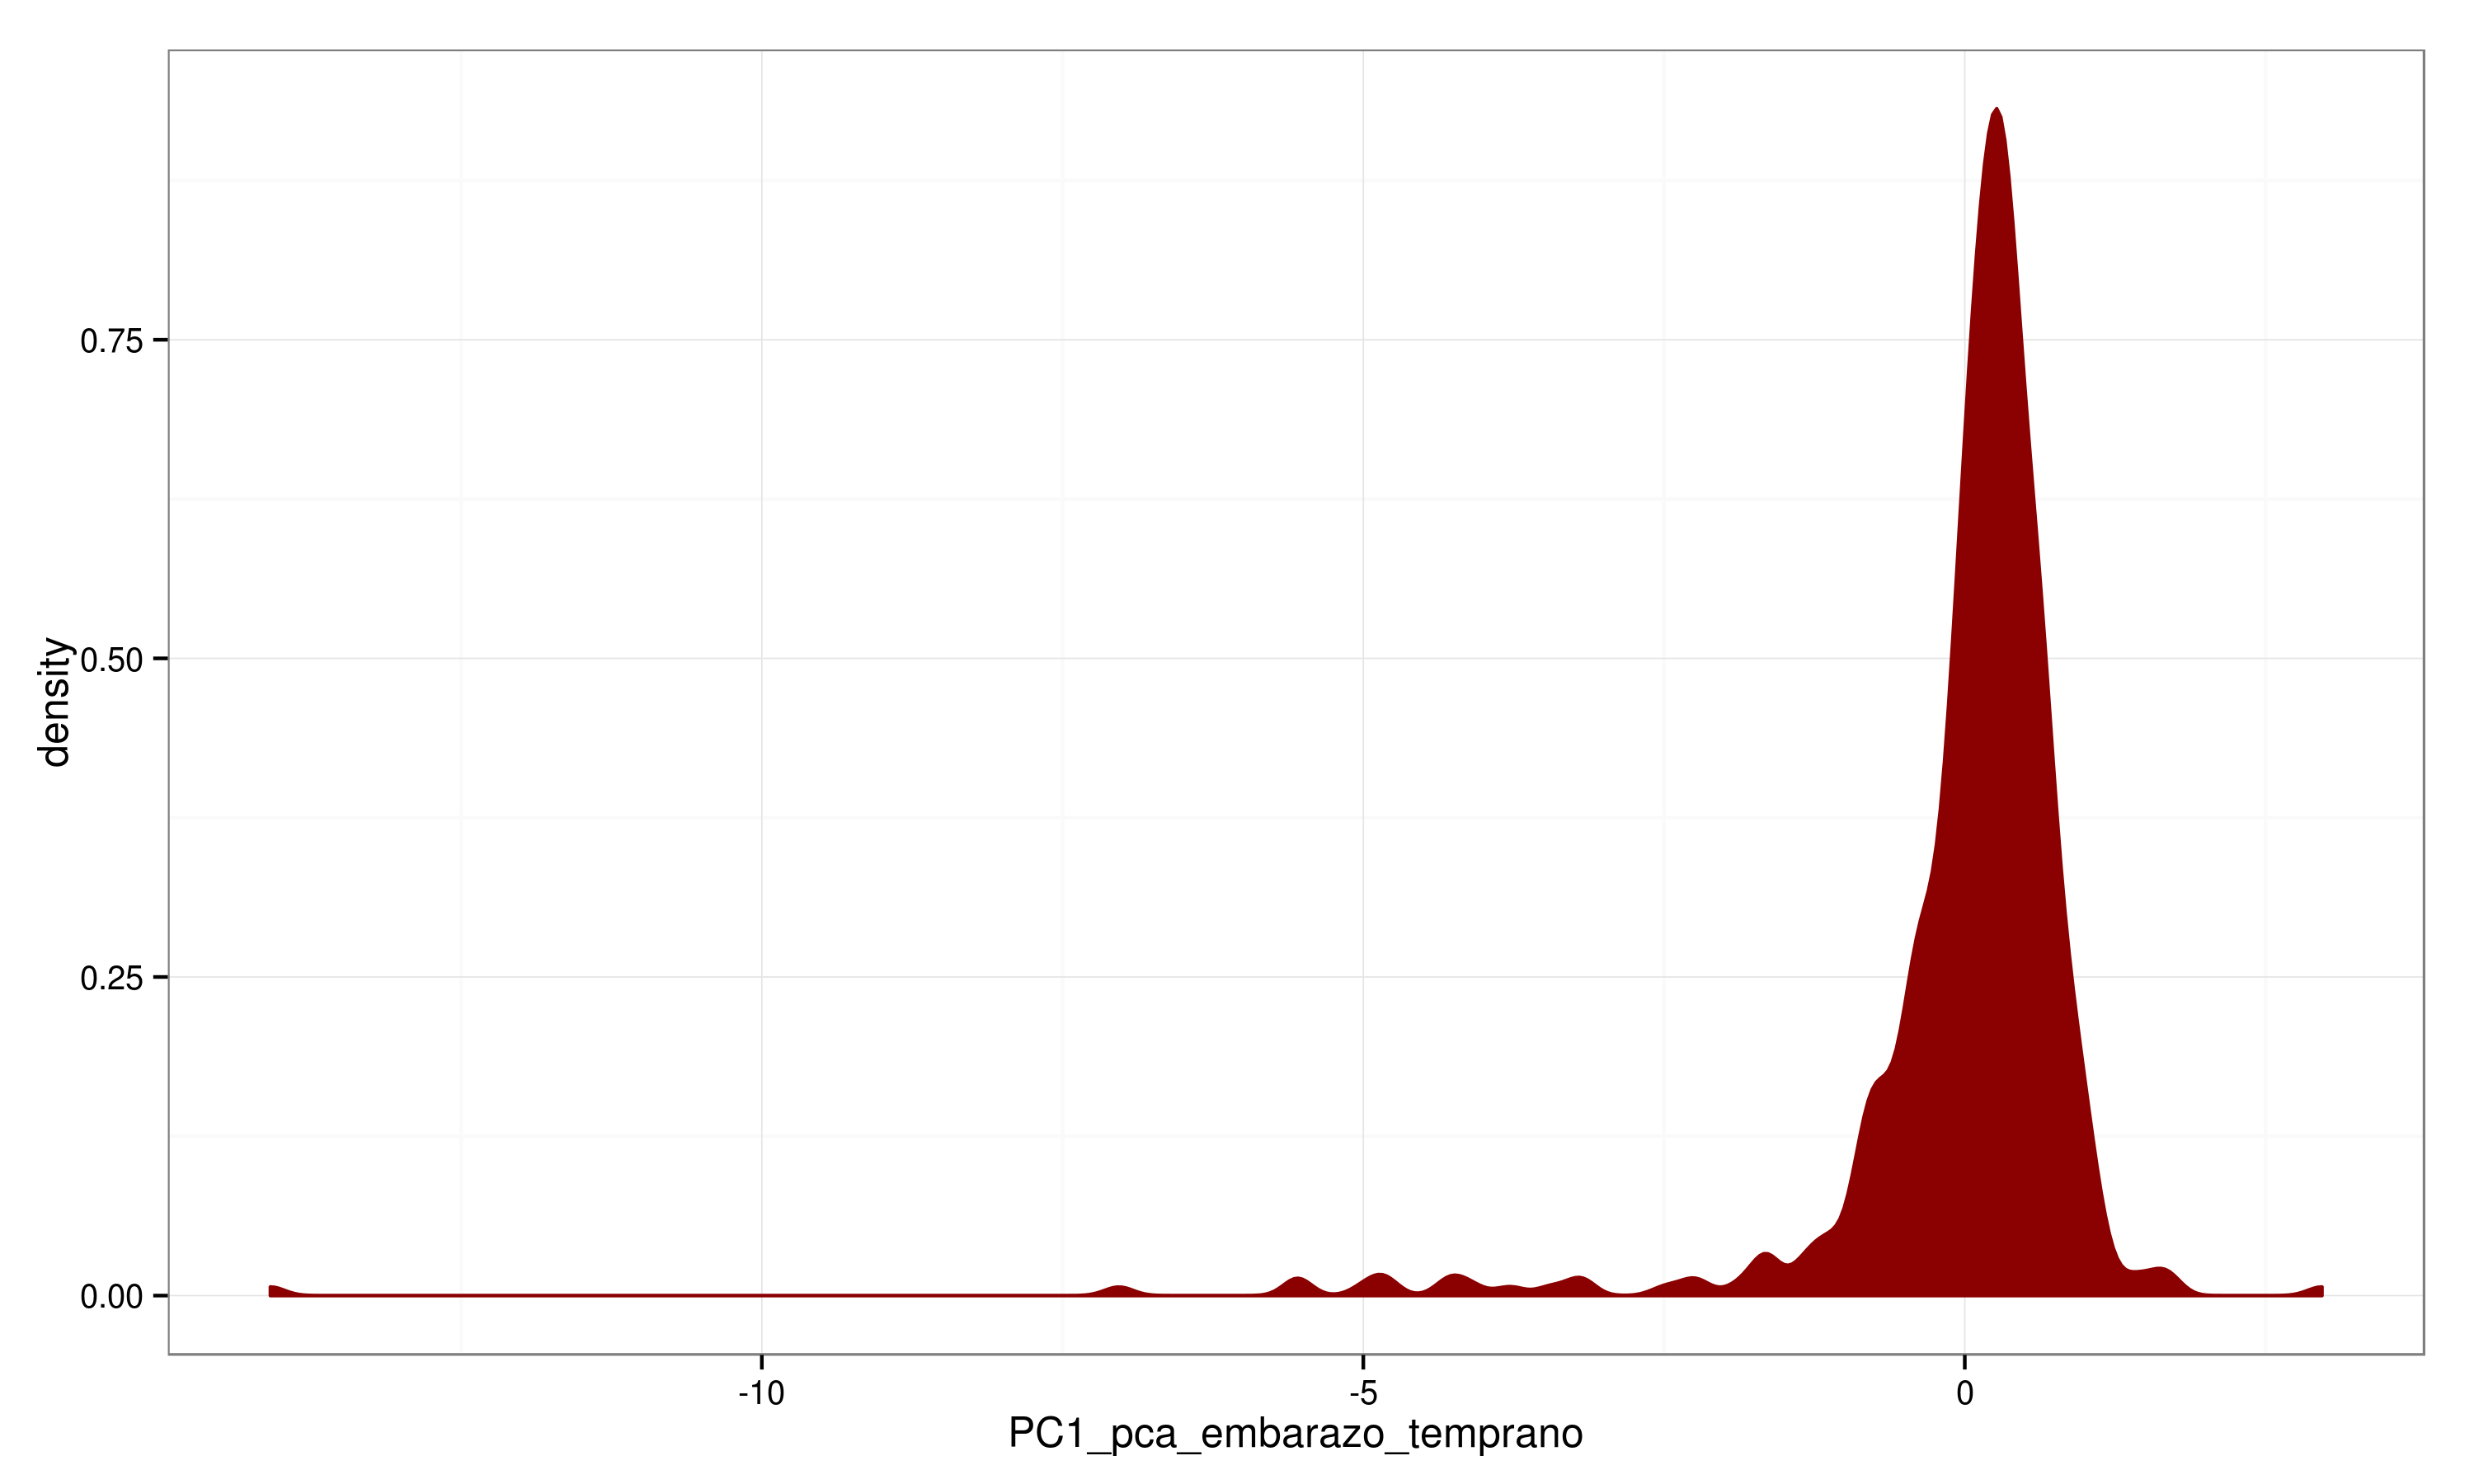
\includegraphics{img/x_density15.png}

\end{frame}

\begin{frame}{Factores de riesgo}

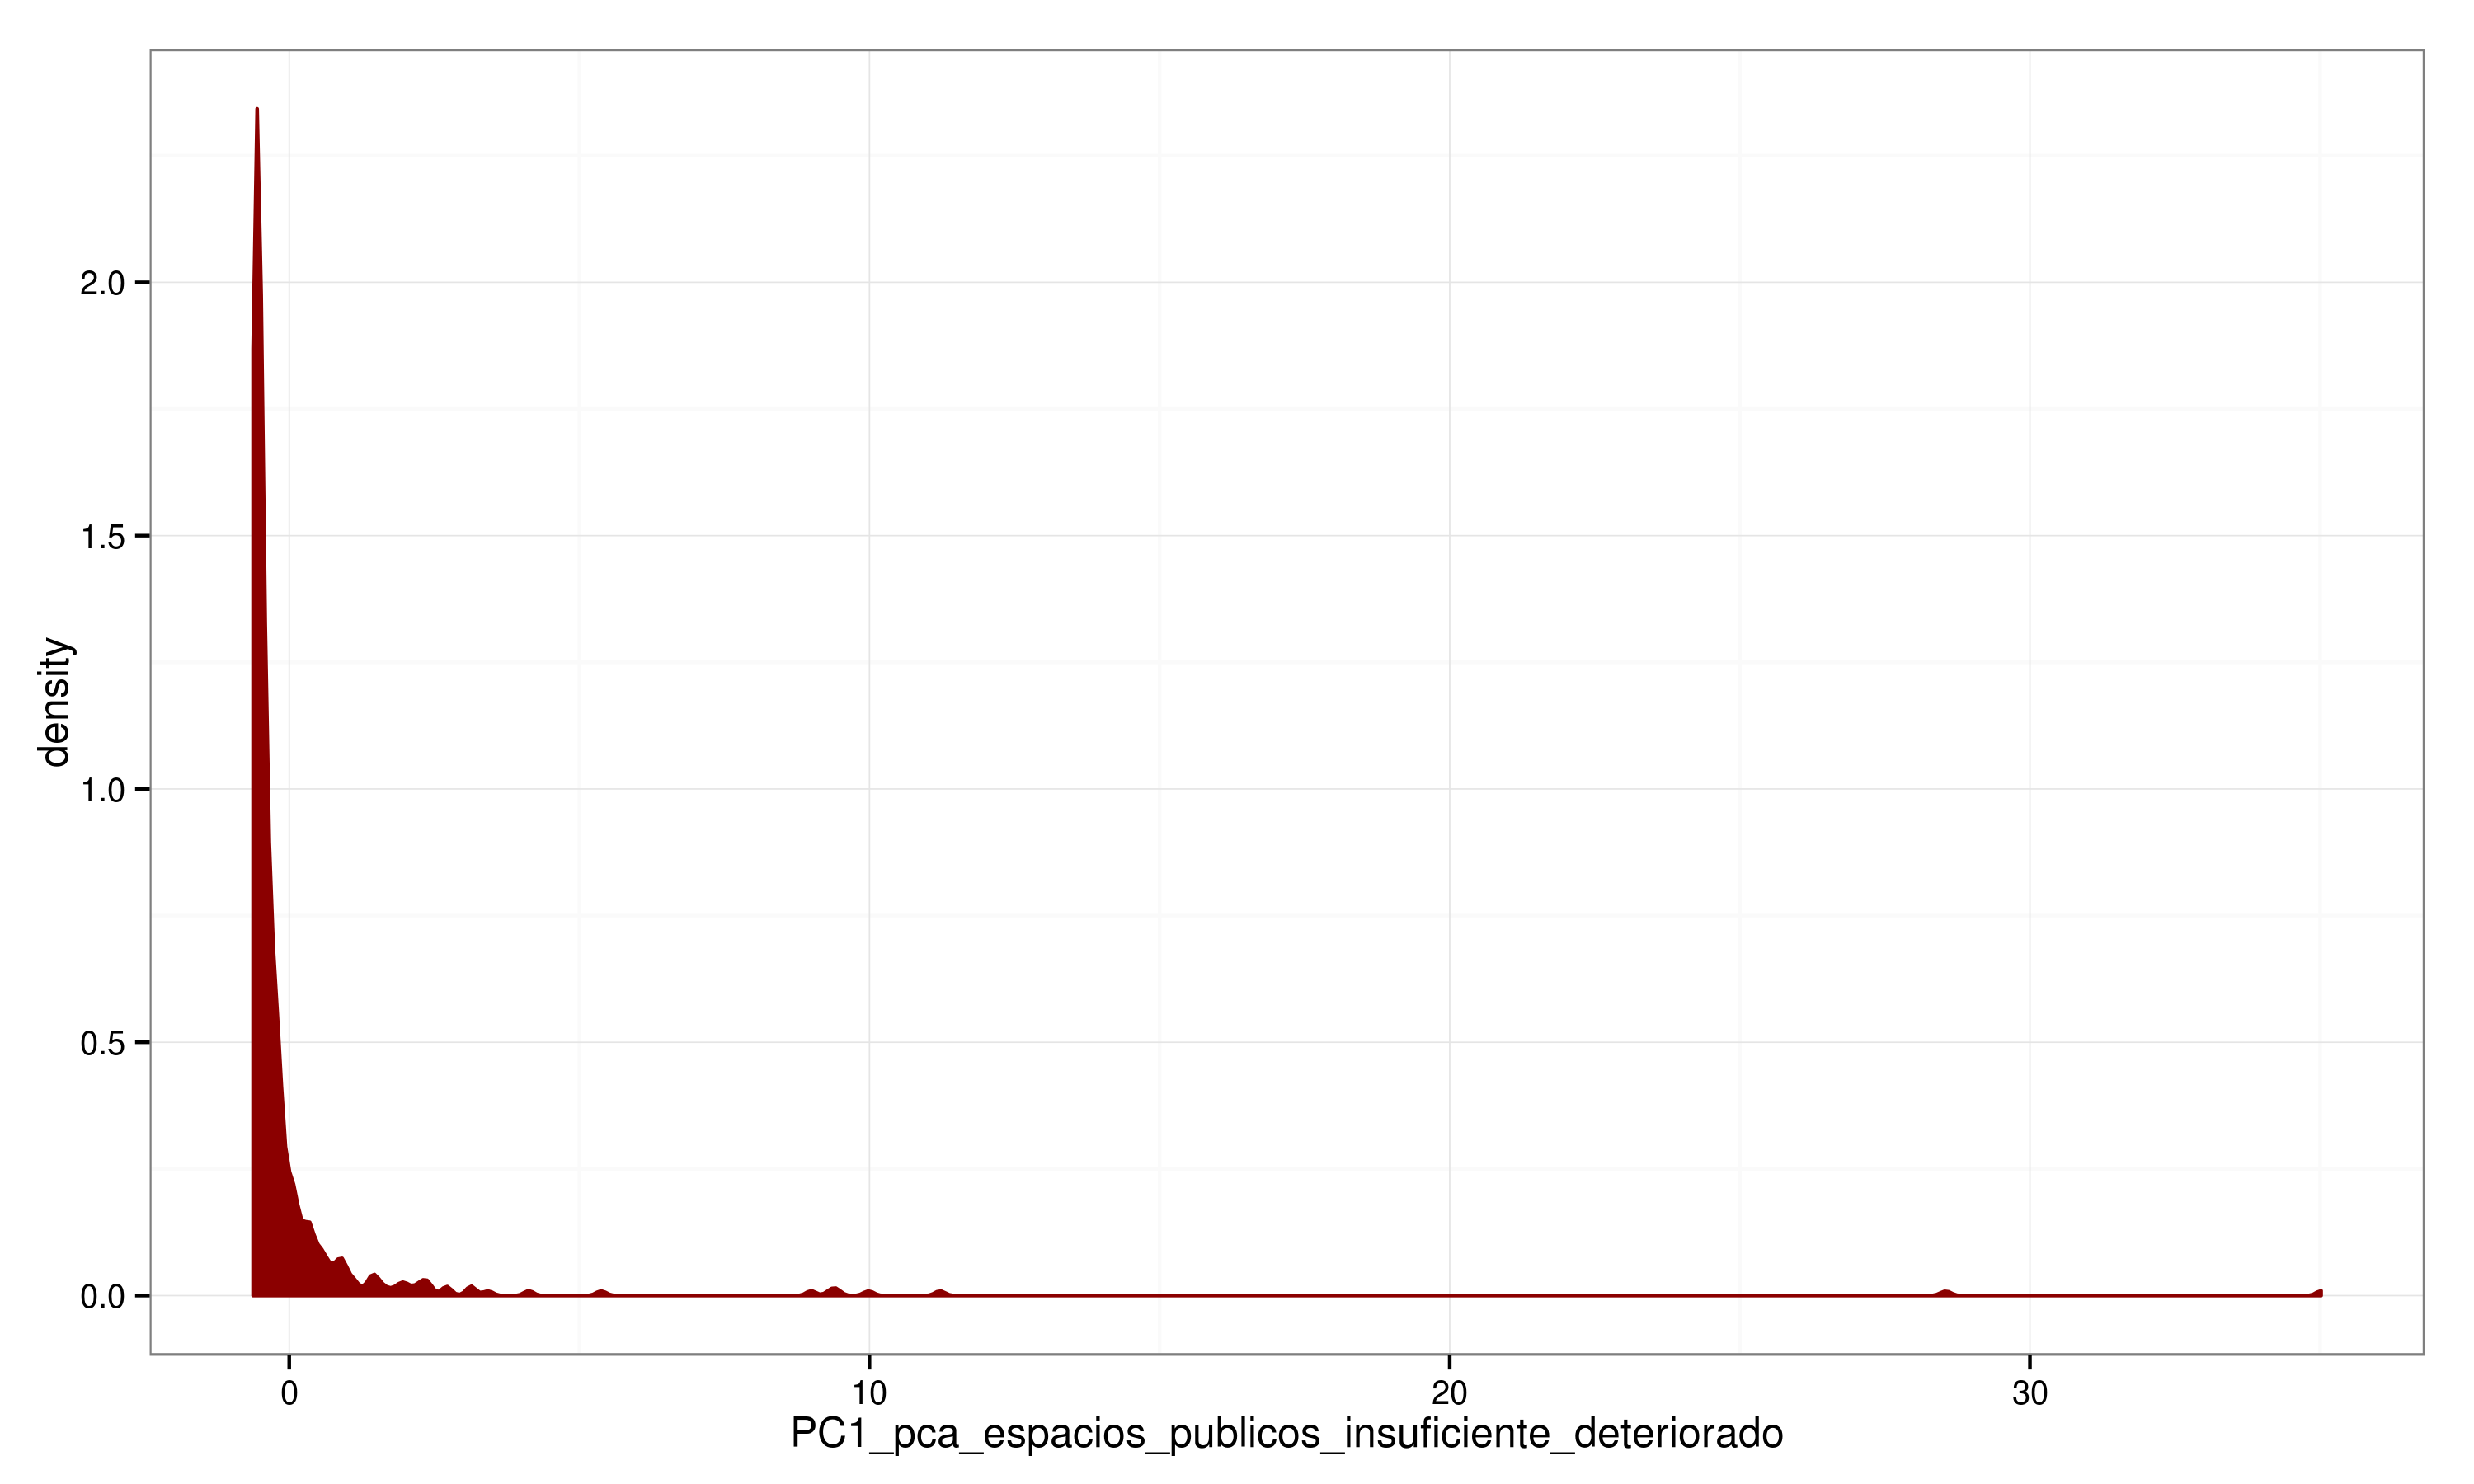
\includegraphics{img/x_density16.png}

\end{frame}

\begin{frame}{Factores de riesgo}

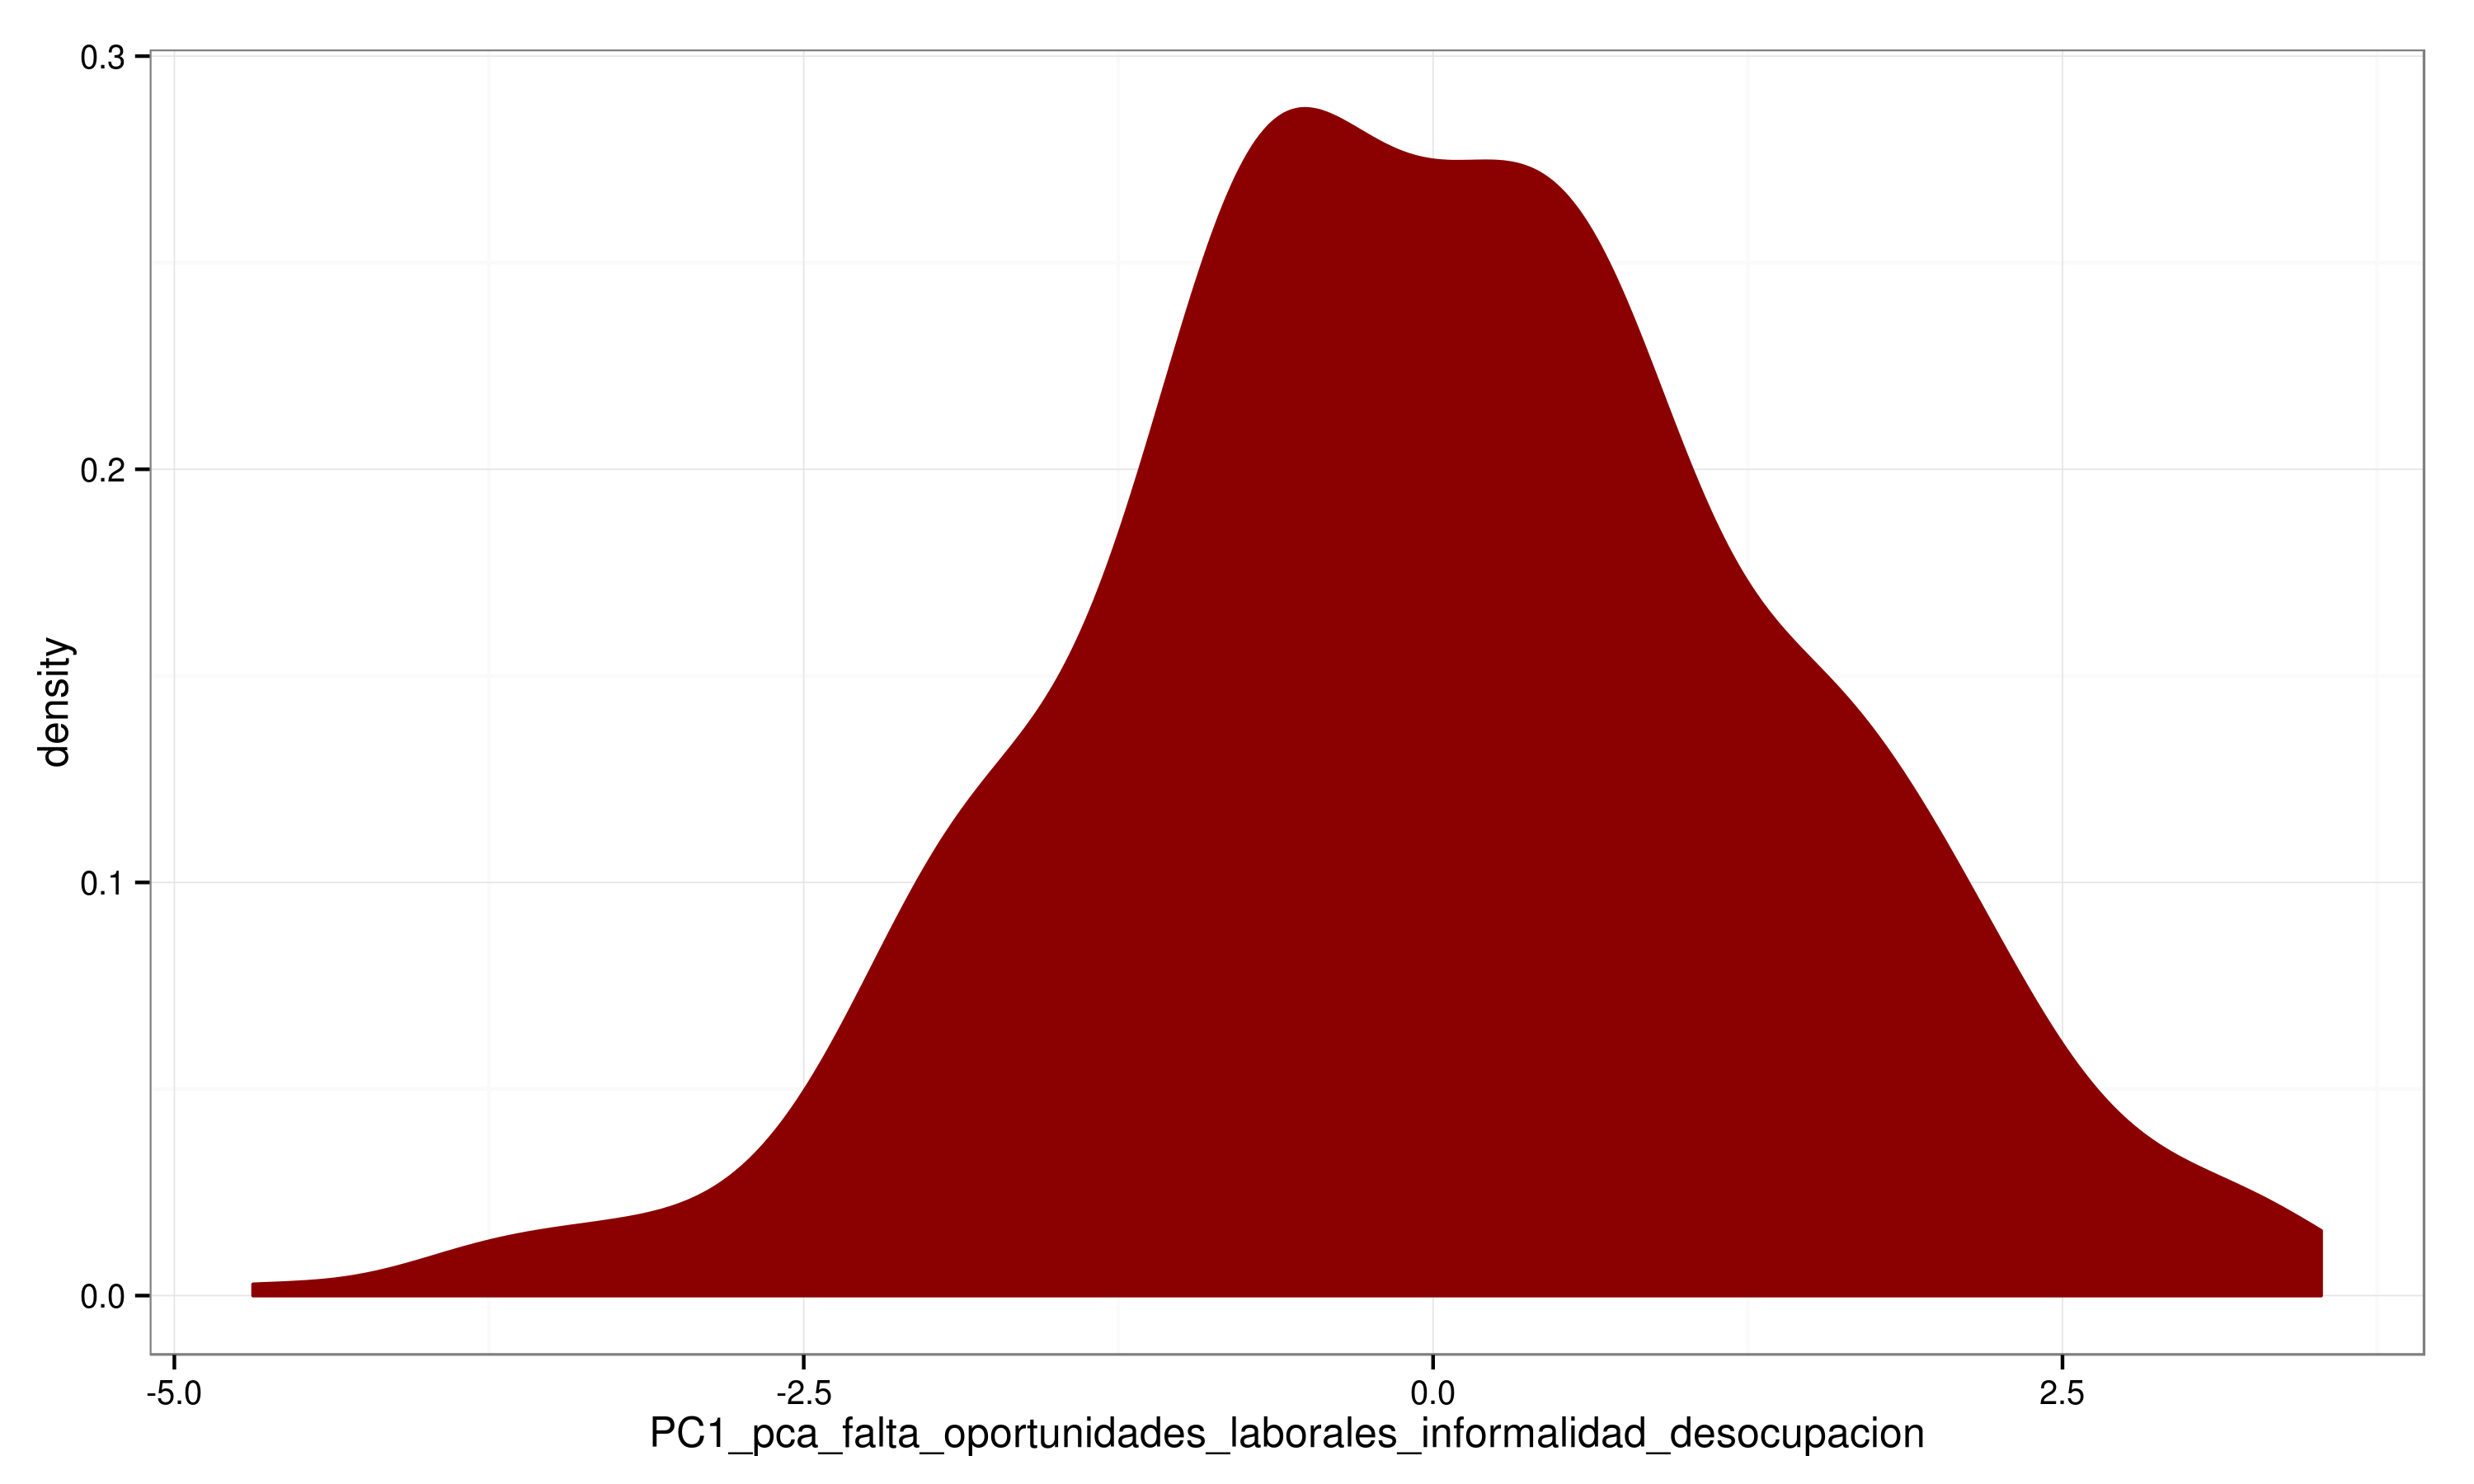
\includegraphics{img/x_density17.png}

\end{frame}

\begin{frame}{Factores de riesgo}

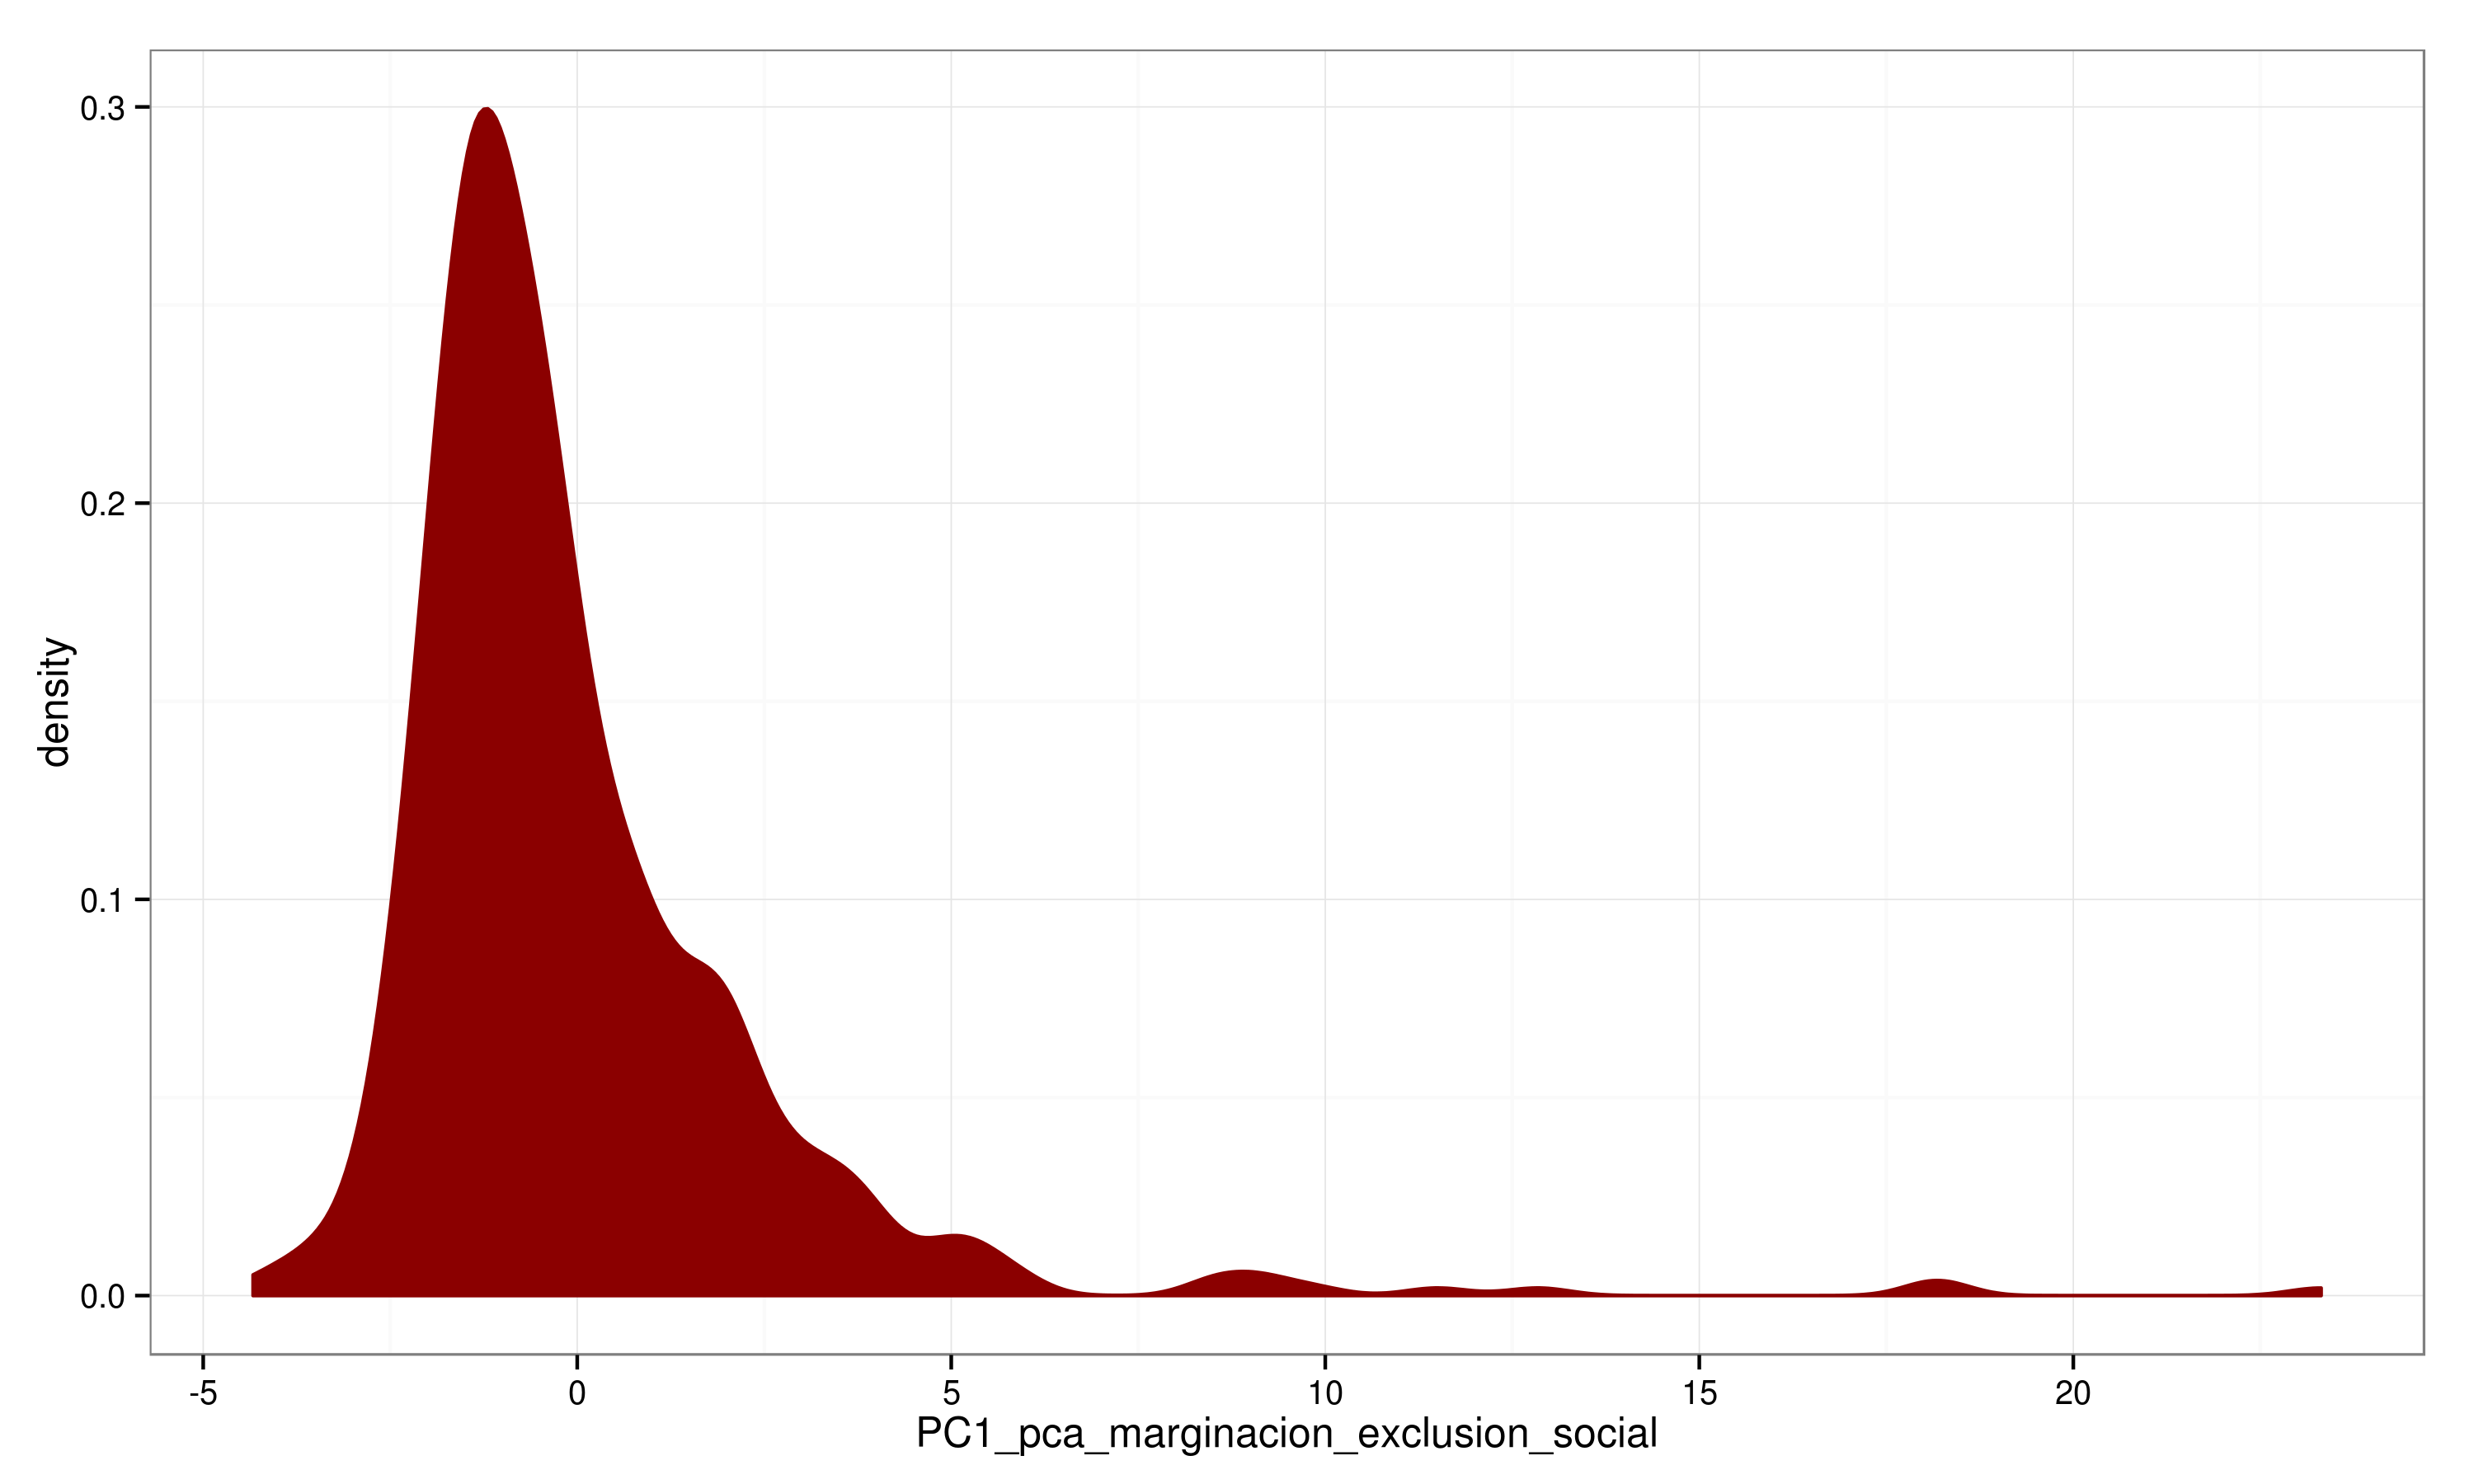
\includegraphics{img/x_density18.png}

\end{frame}

\begin{frame}{Factores de riesgo}

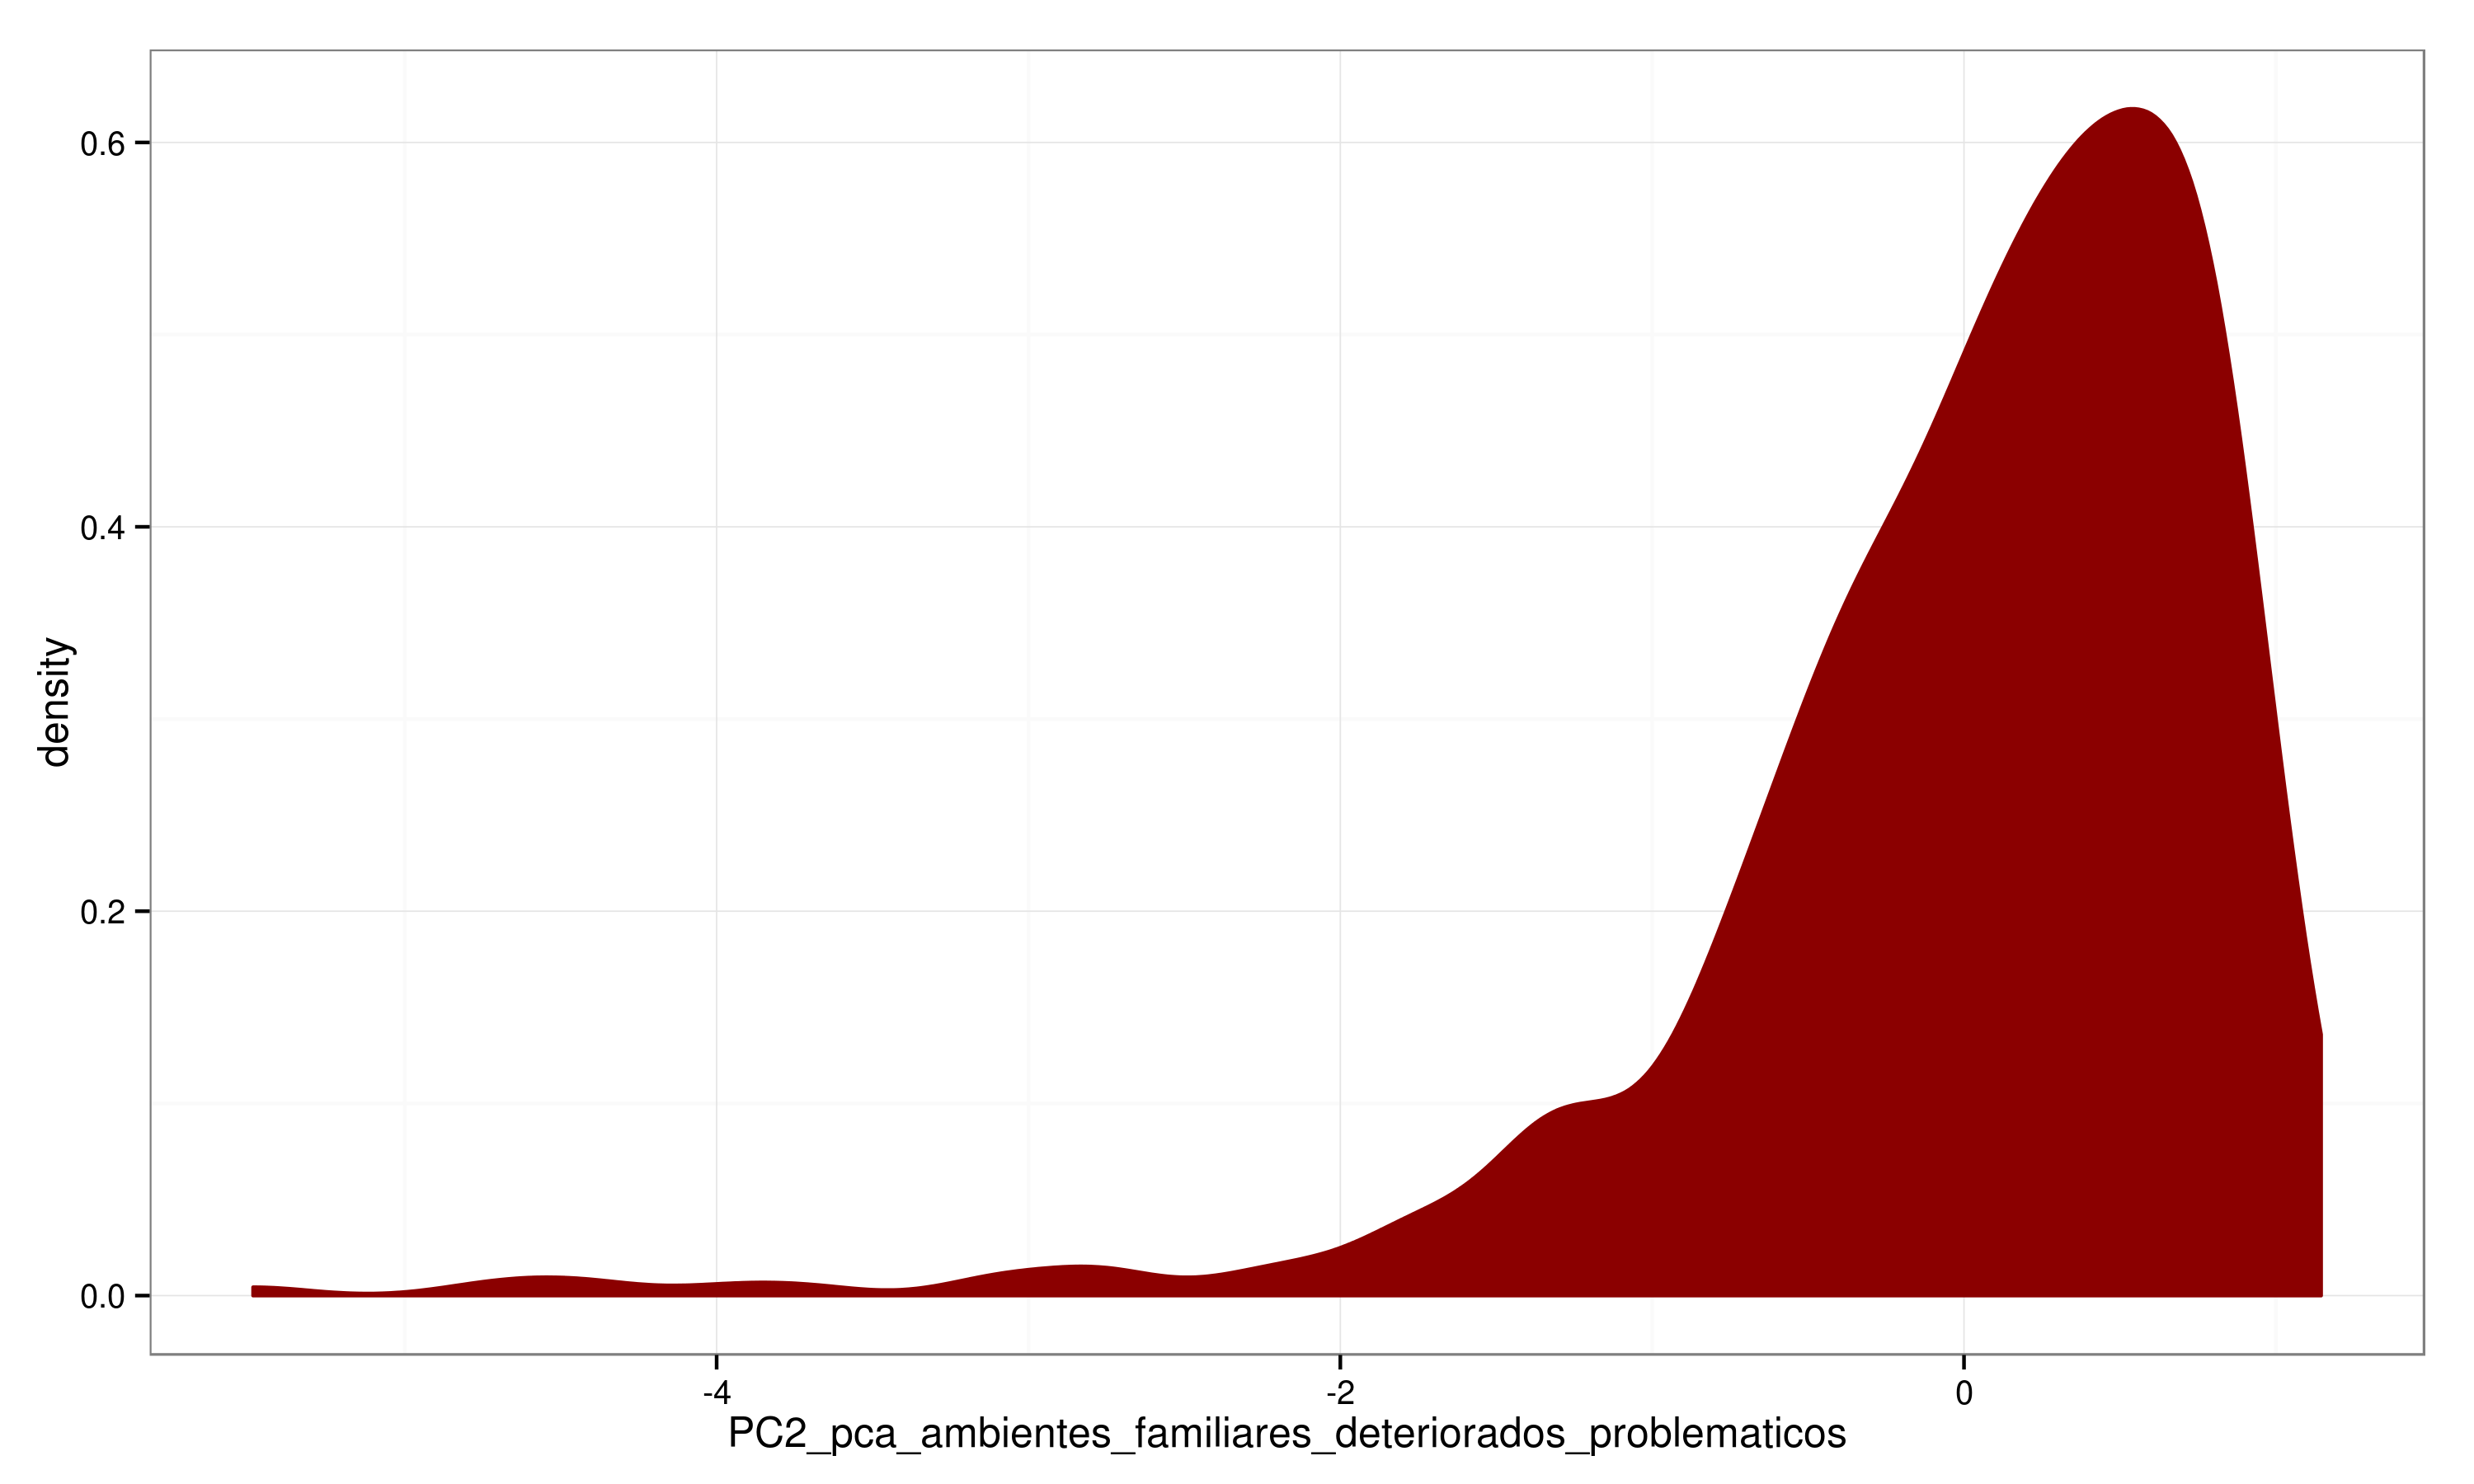
\includegraphics{img/x_density19.png}

\end{frame}

\begin{frame}{Factores de riesgo}

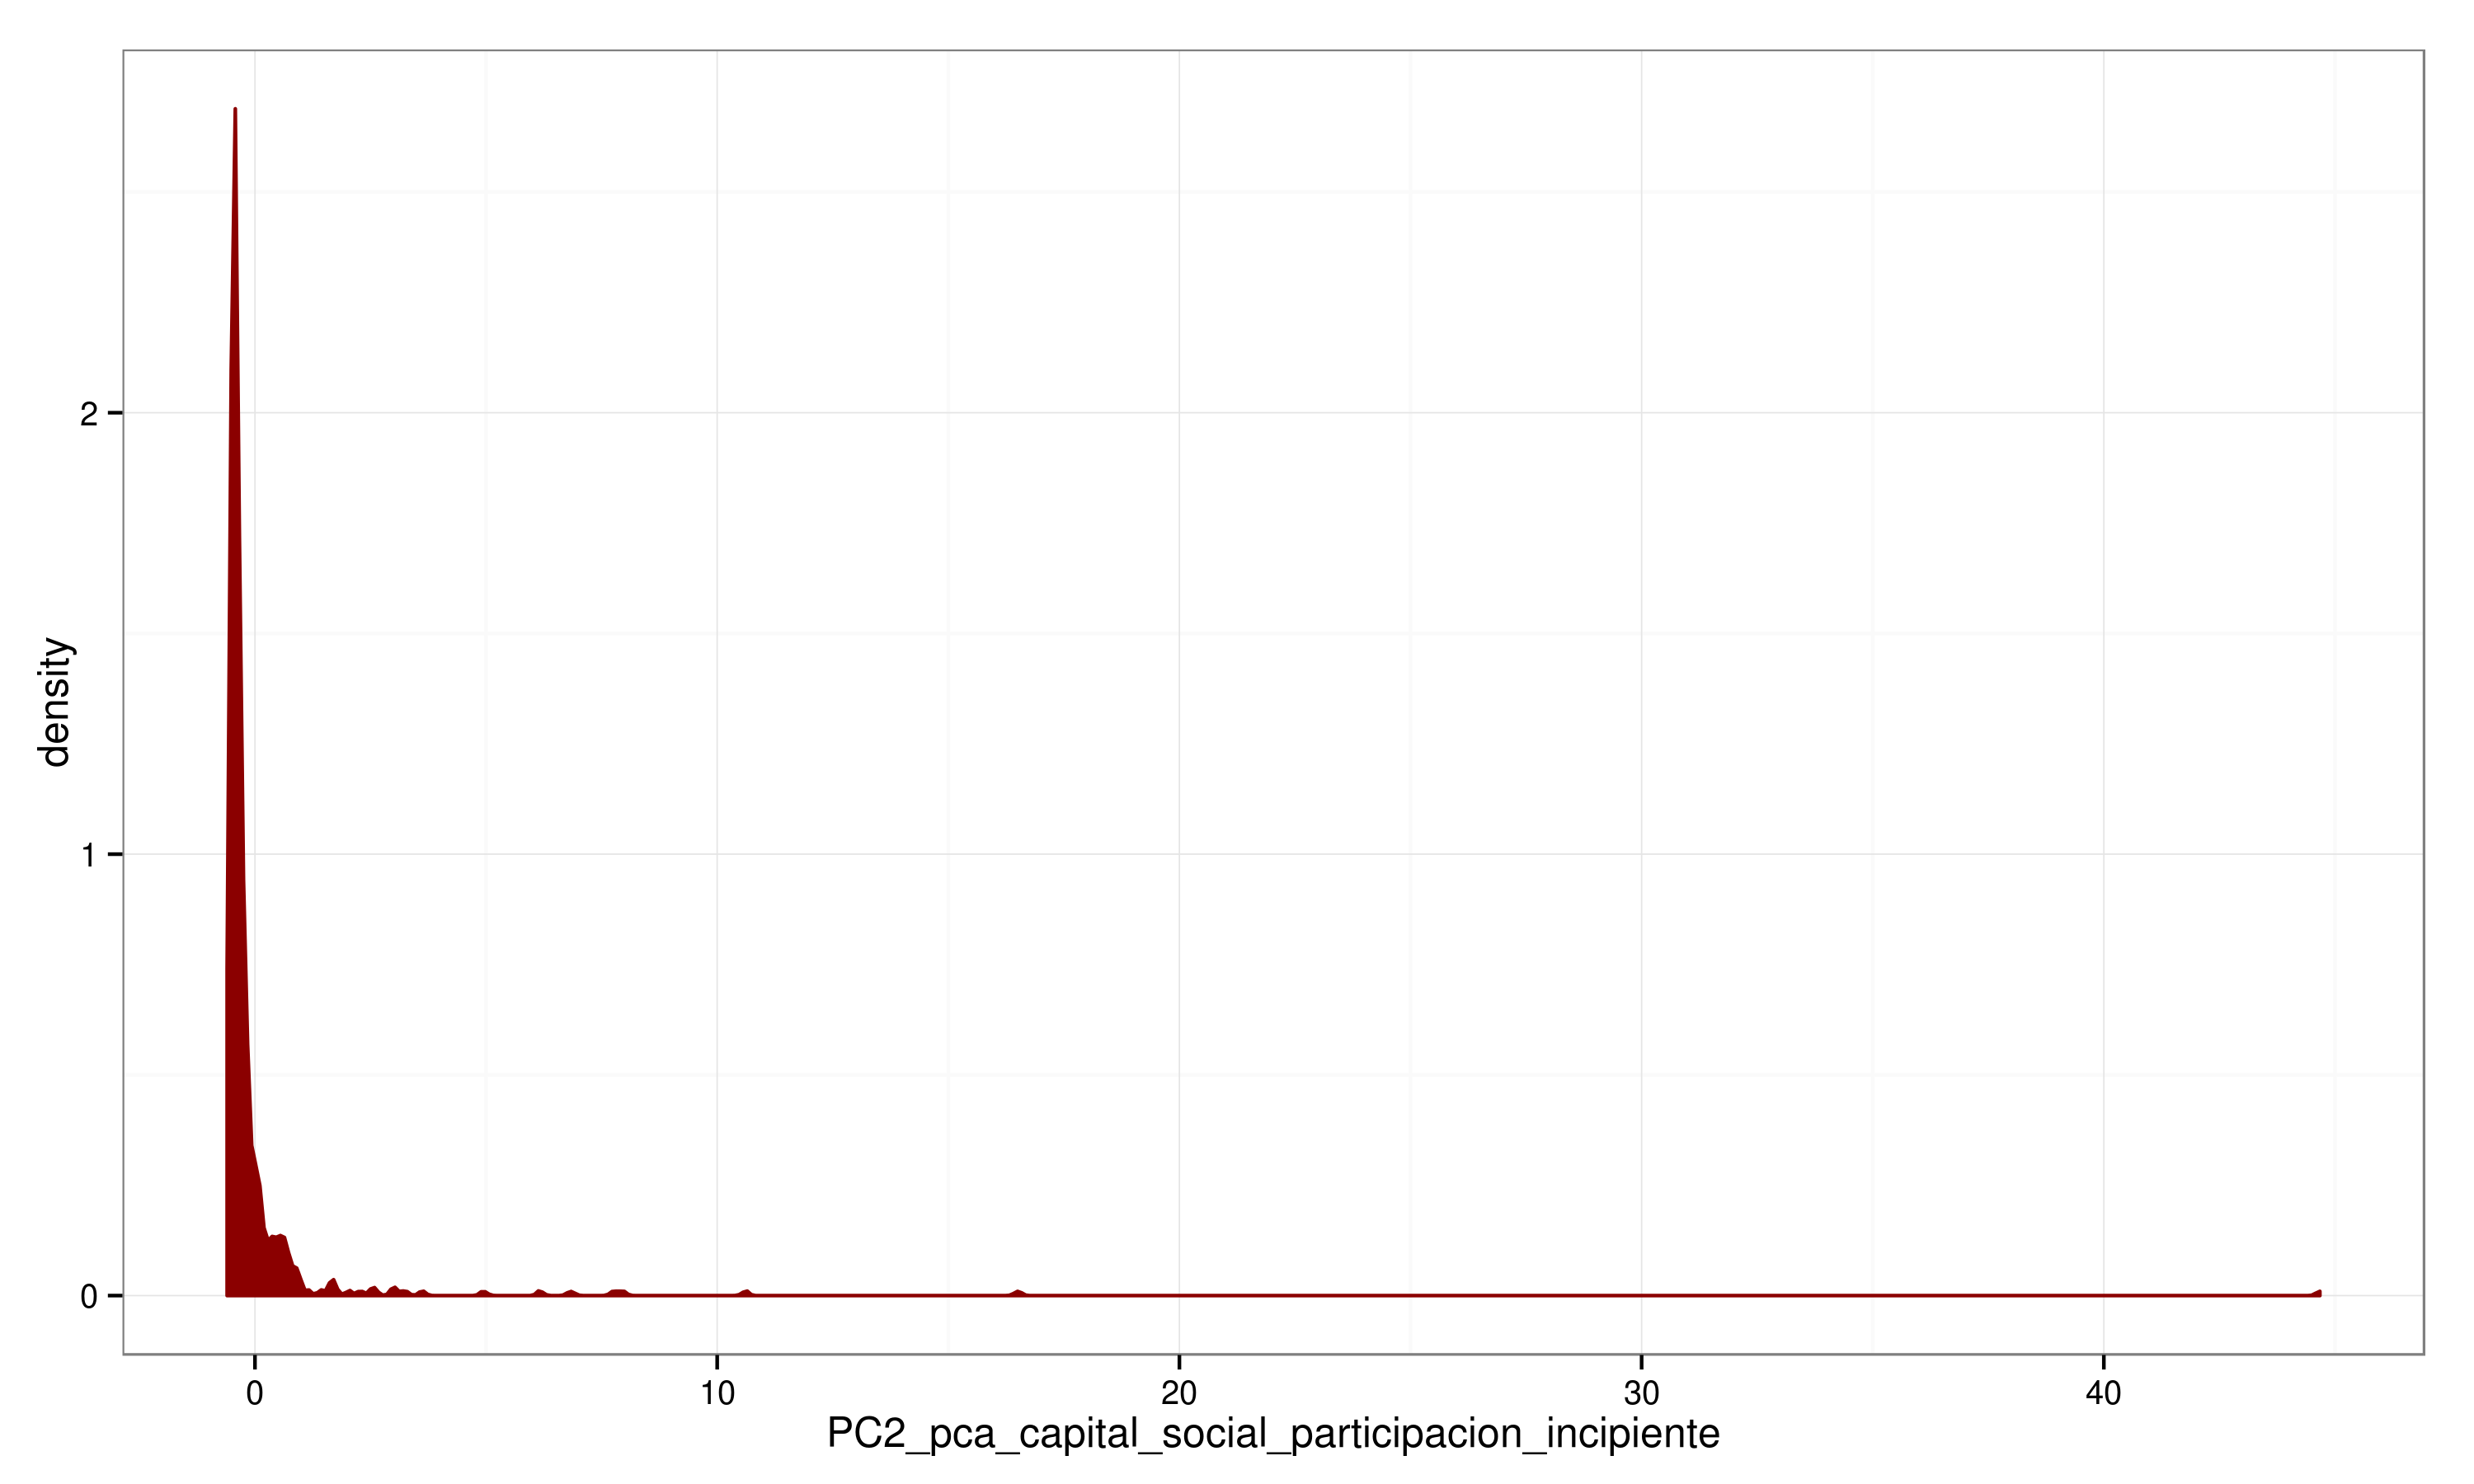
\includegraphics{img/x_density20.png}

\end{frame}

\begin{frame}{Factores de riesgo}

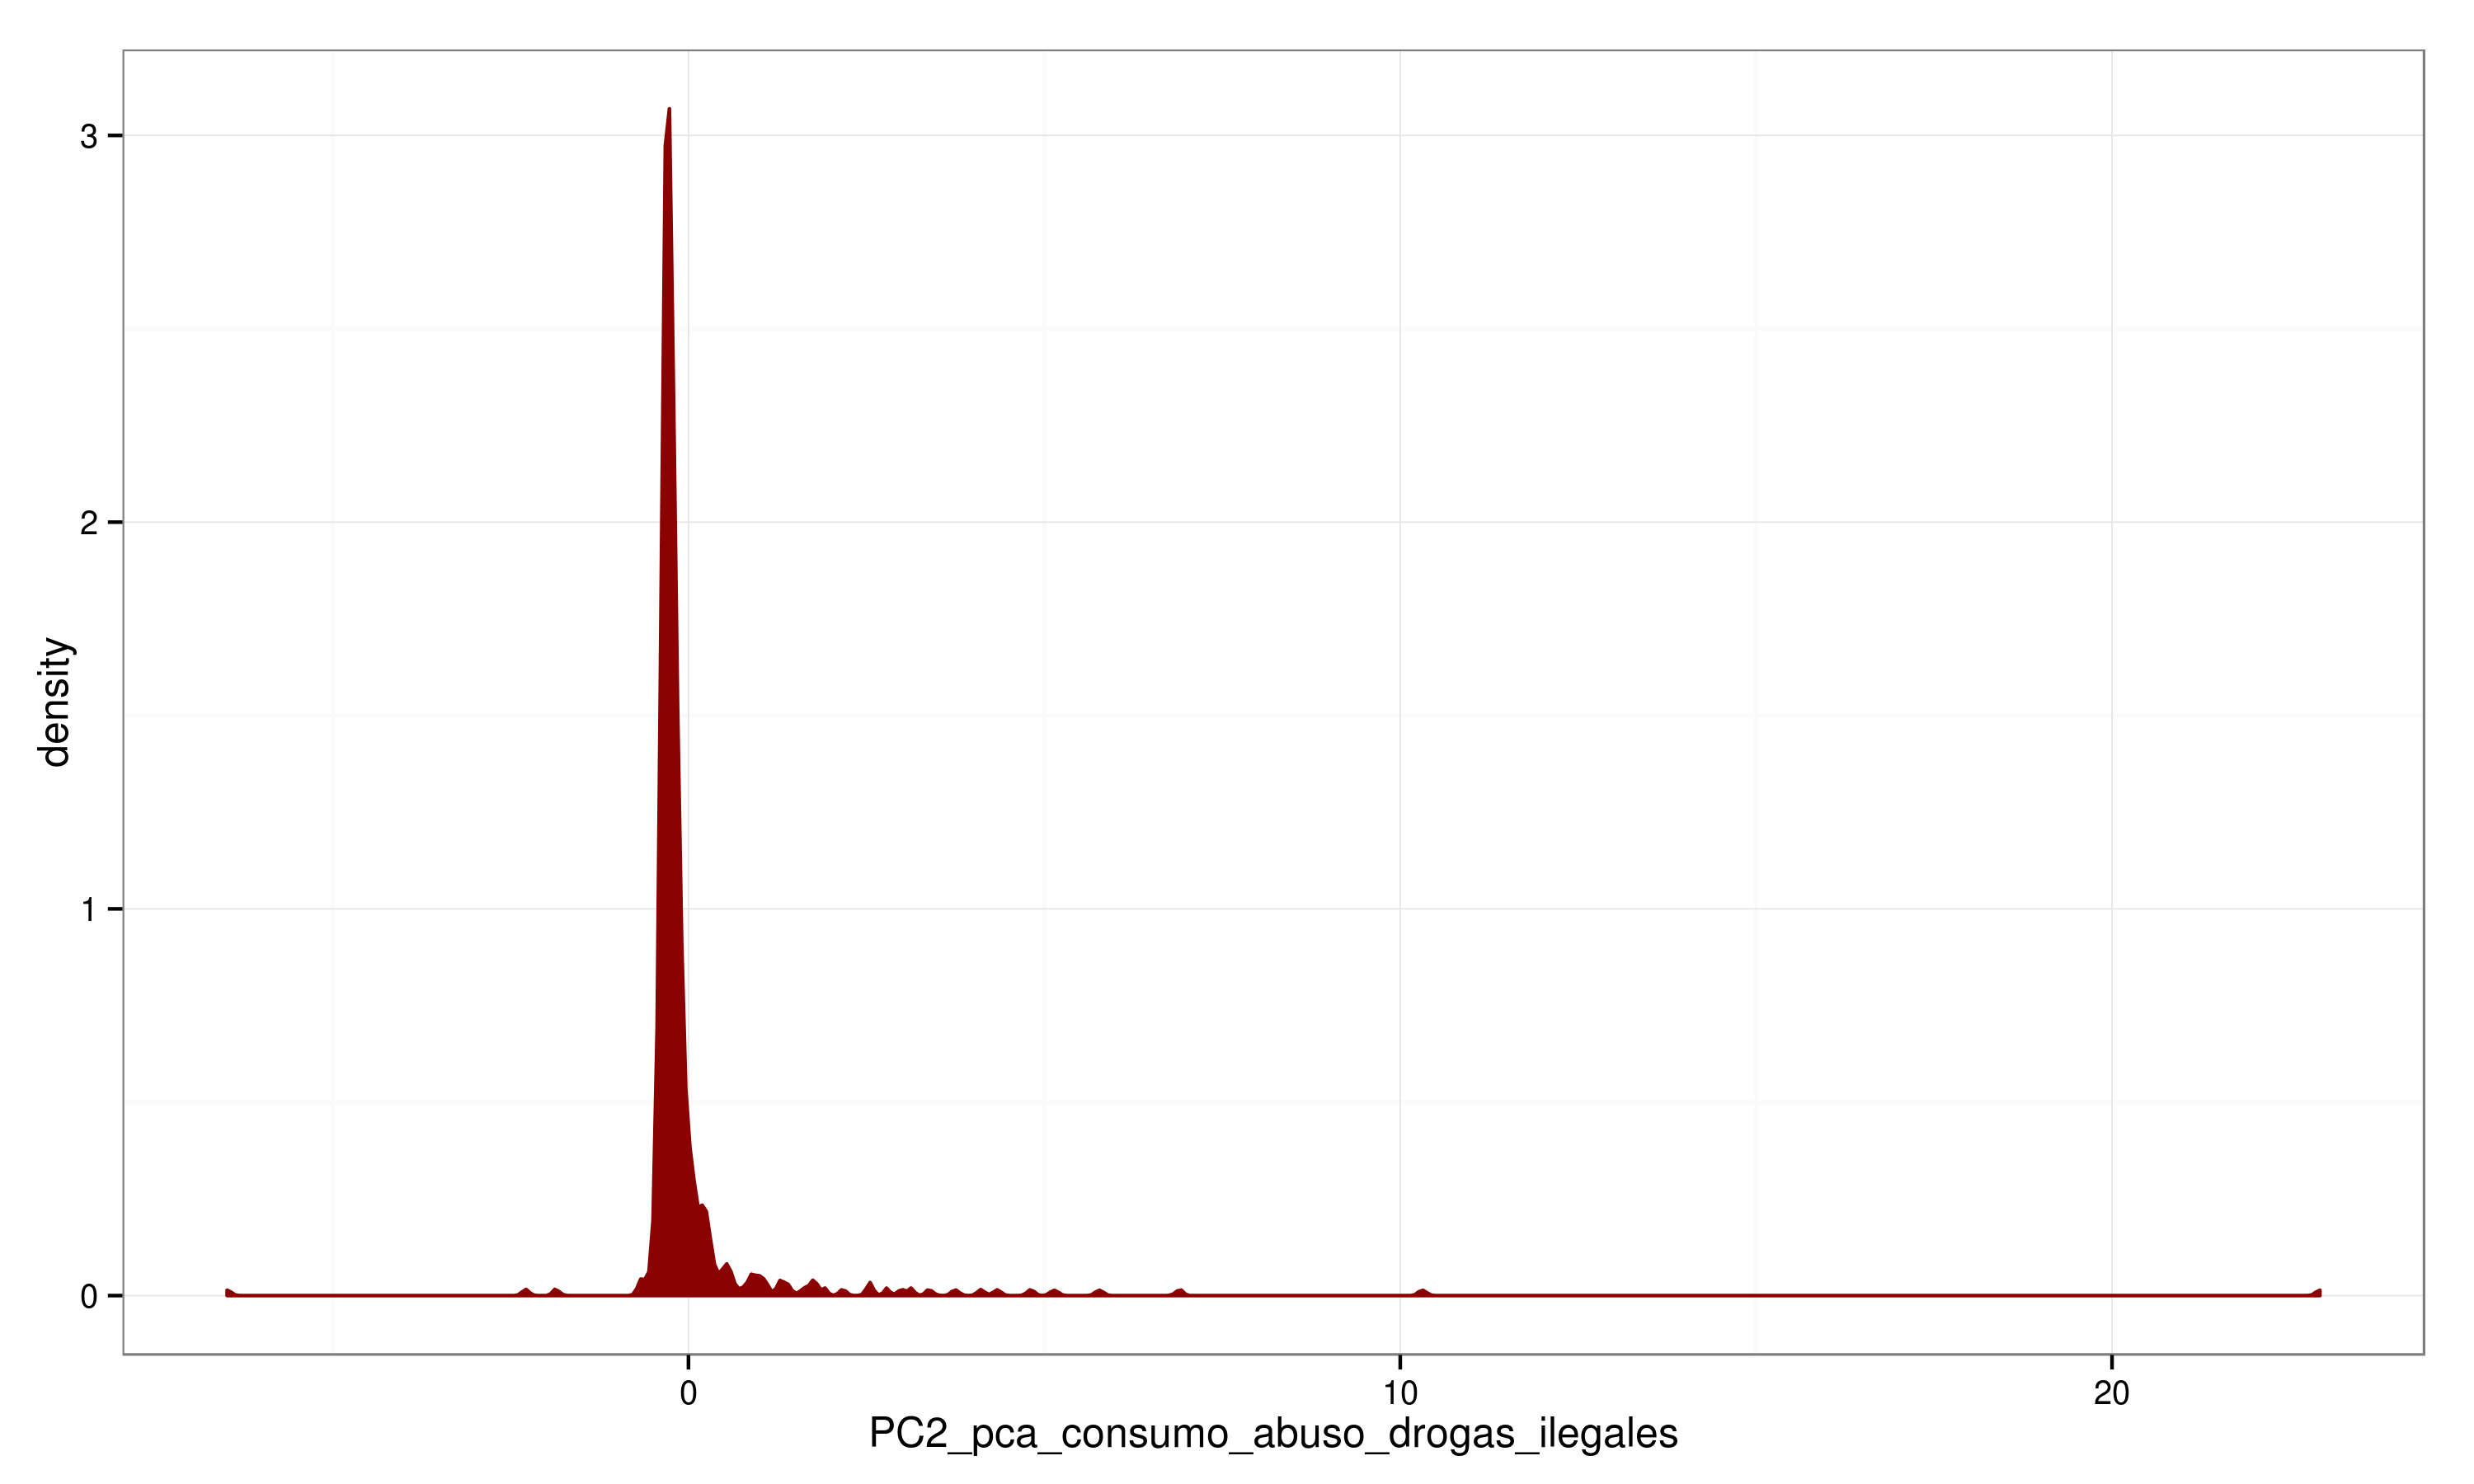
\includegraphics{img/x_density21.png}

\end{frame}

\begin{frame}{Factores de riesgo}

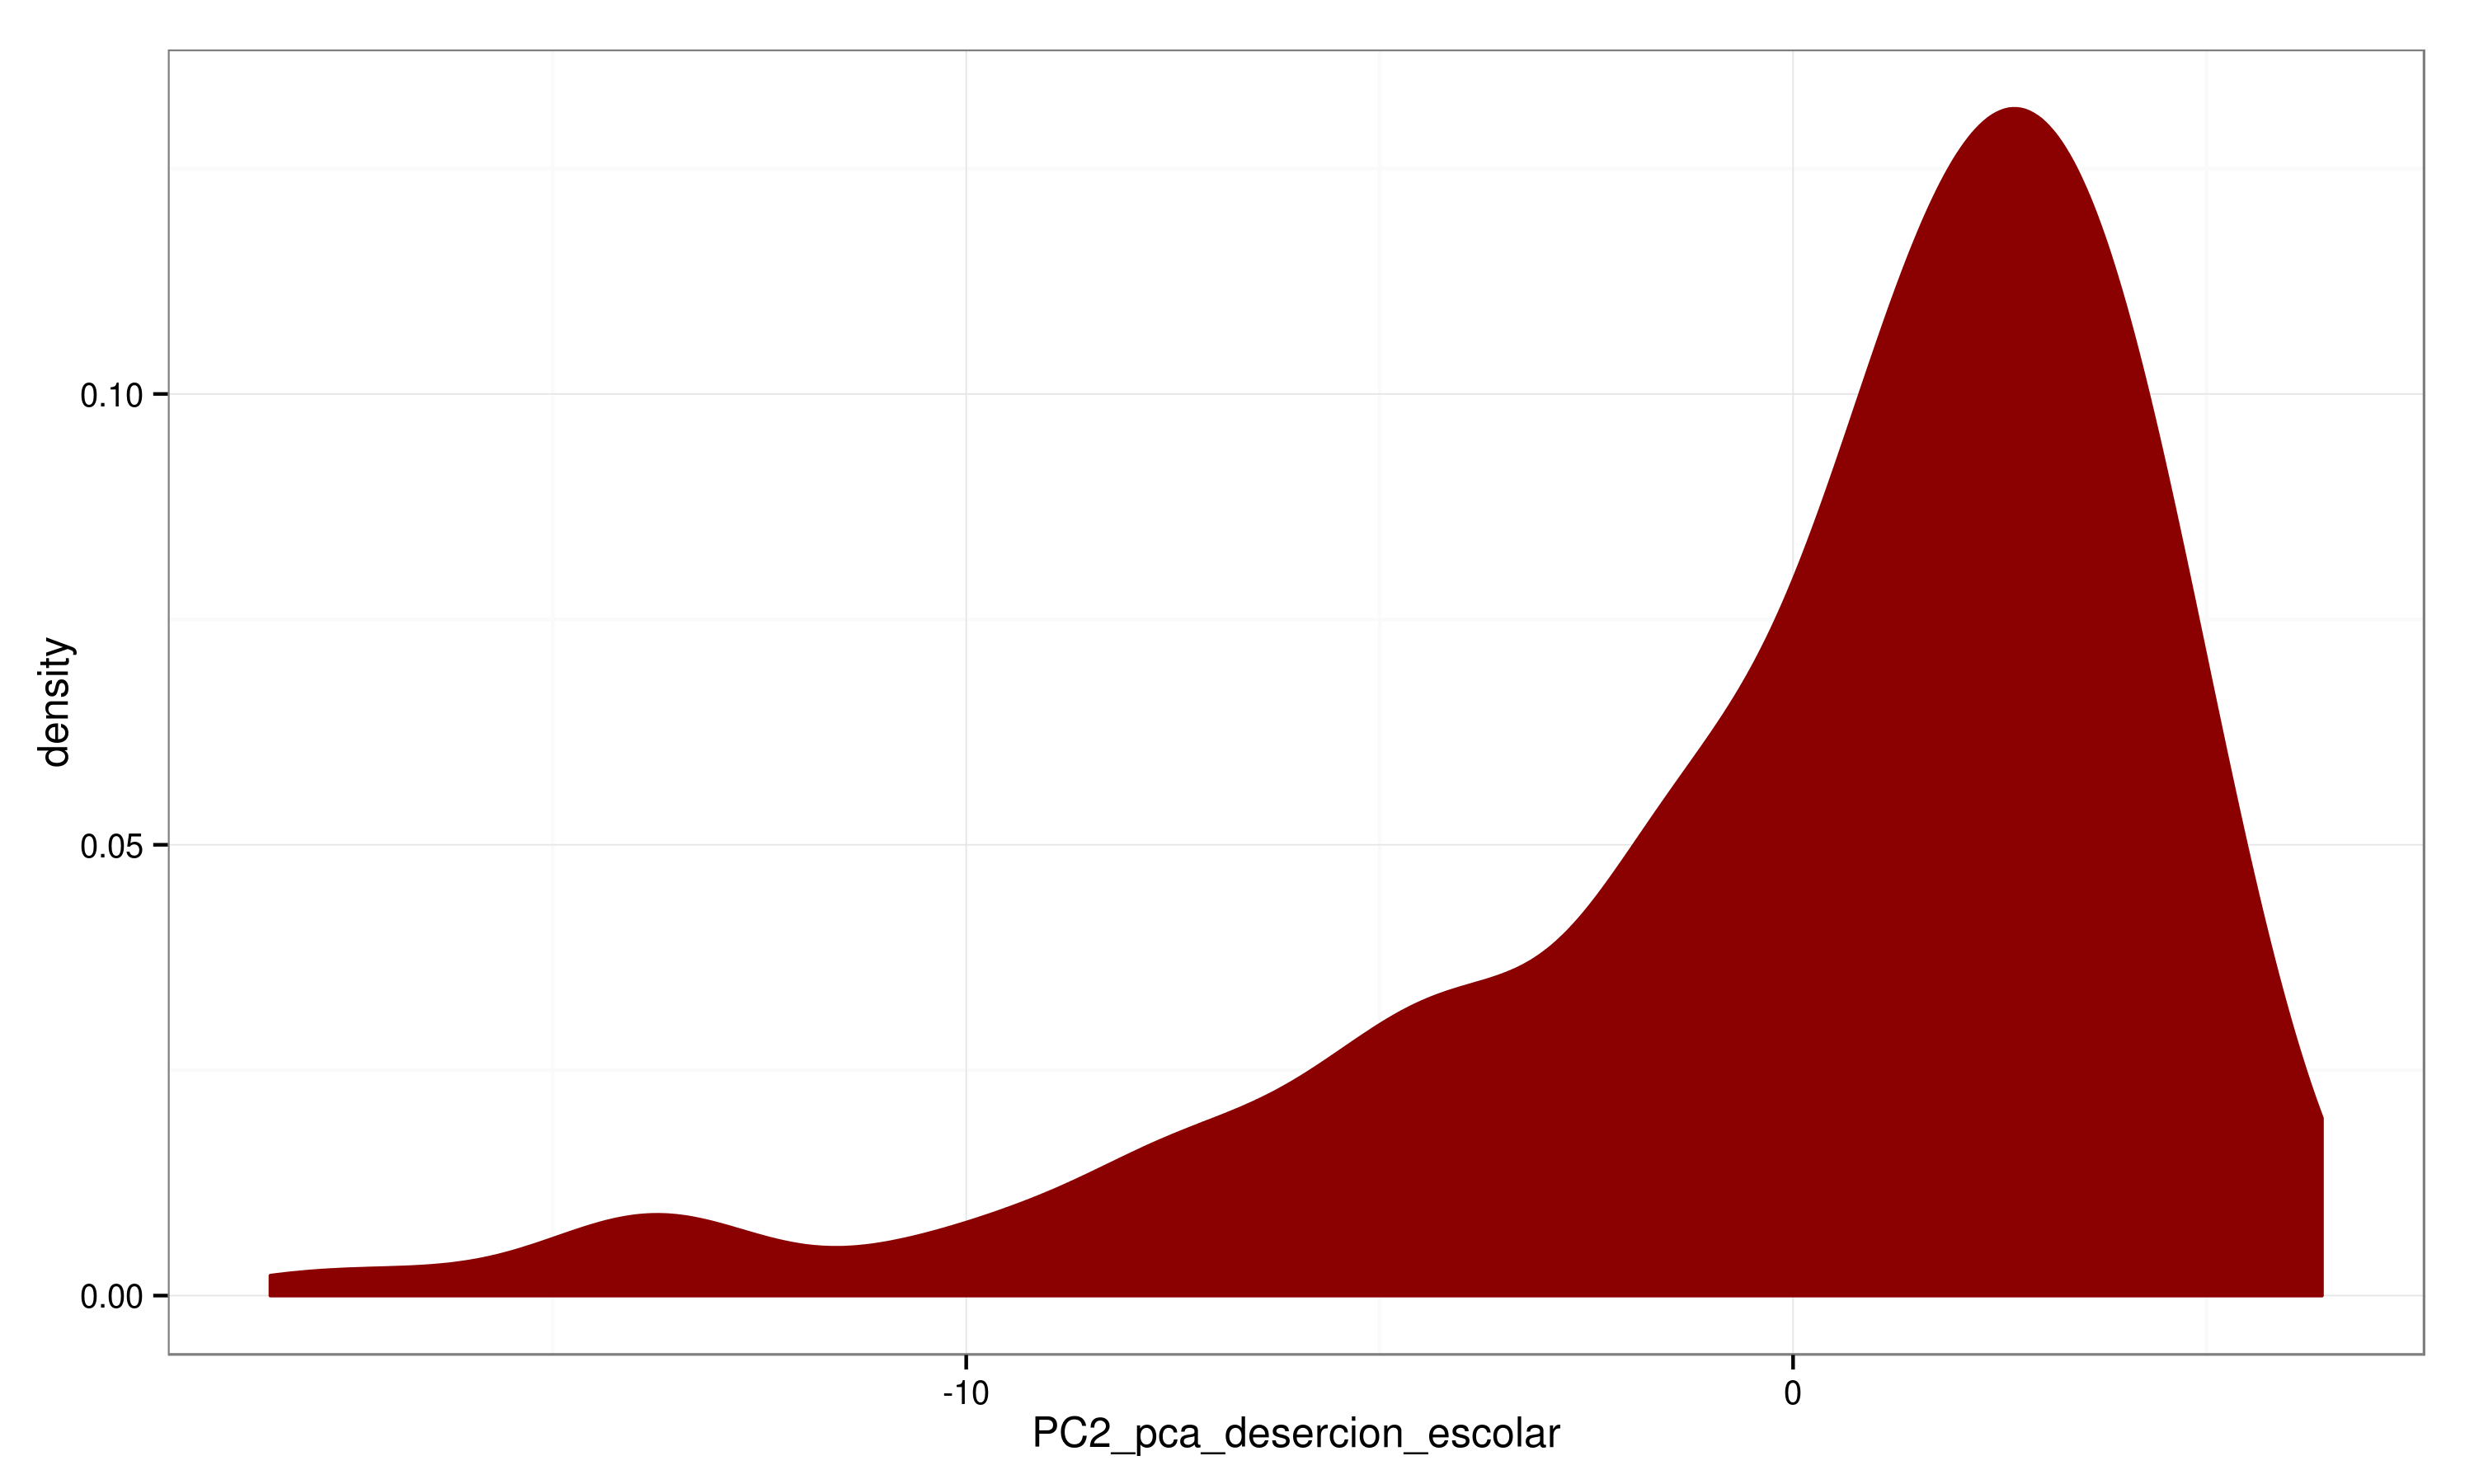
\includegraphics{img/x_density22.png}

\end{frame}

\begin{frame}{Factores de riesgo}

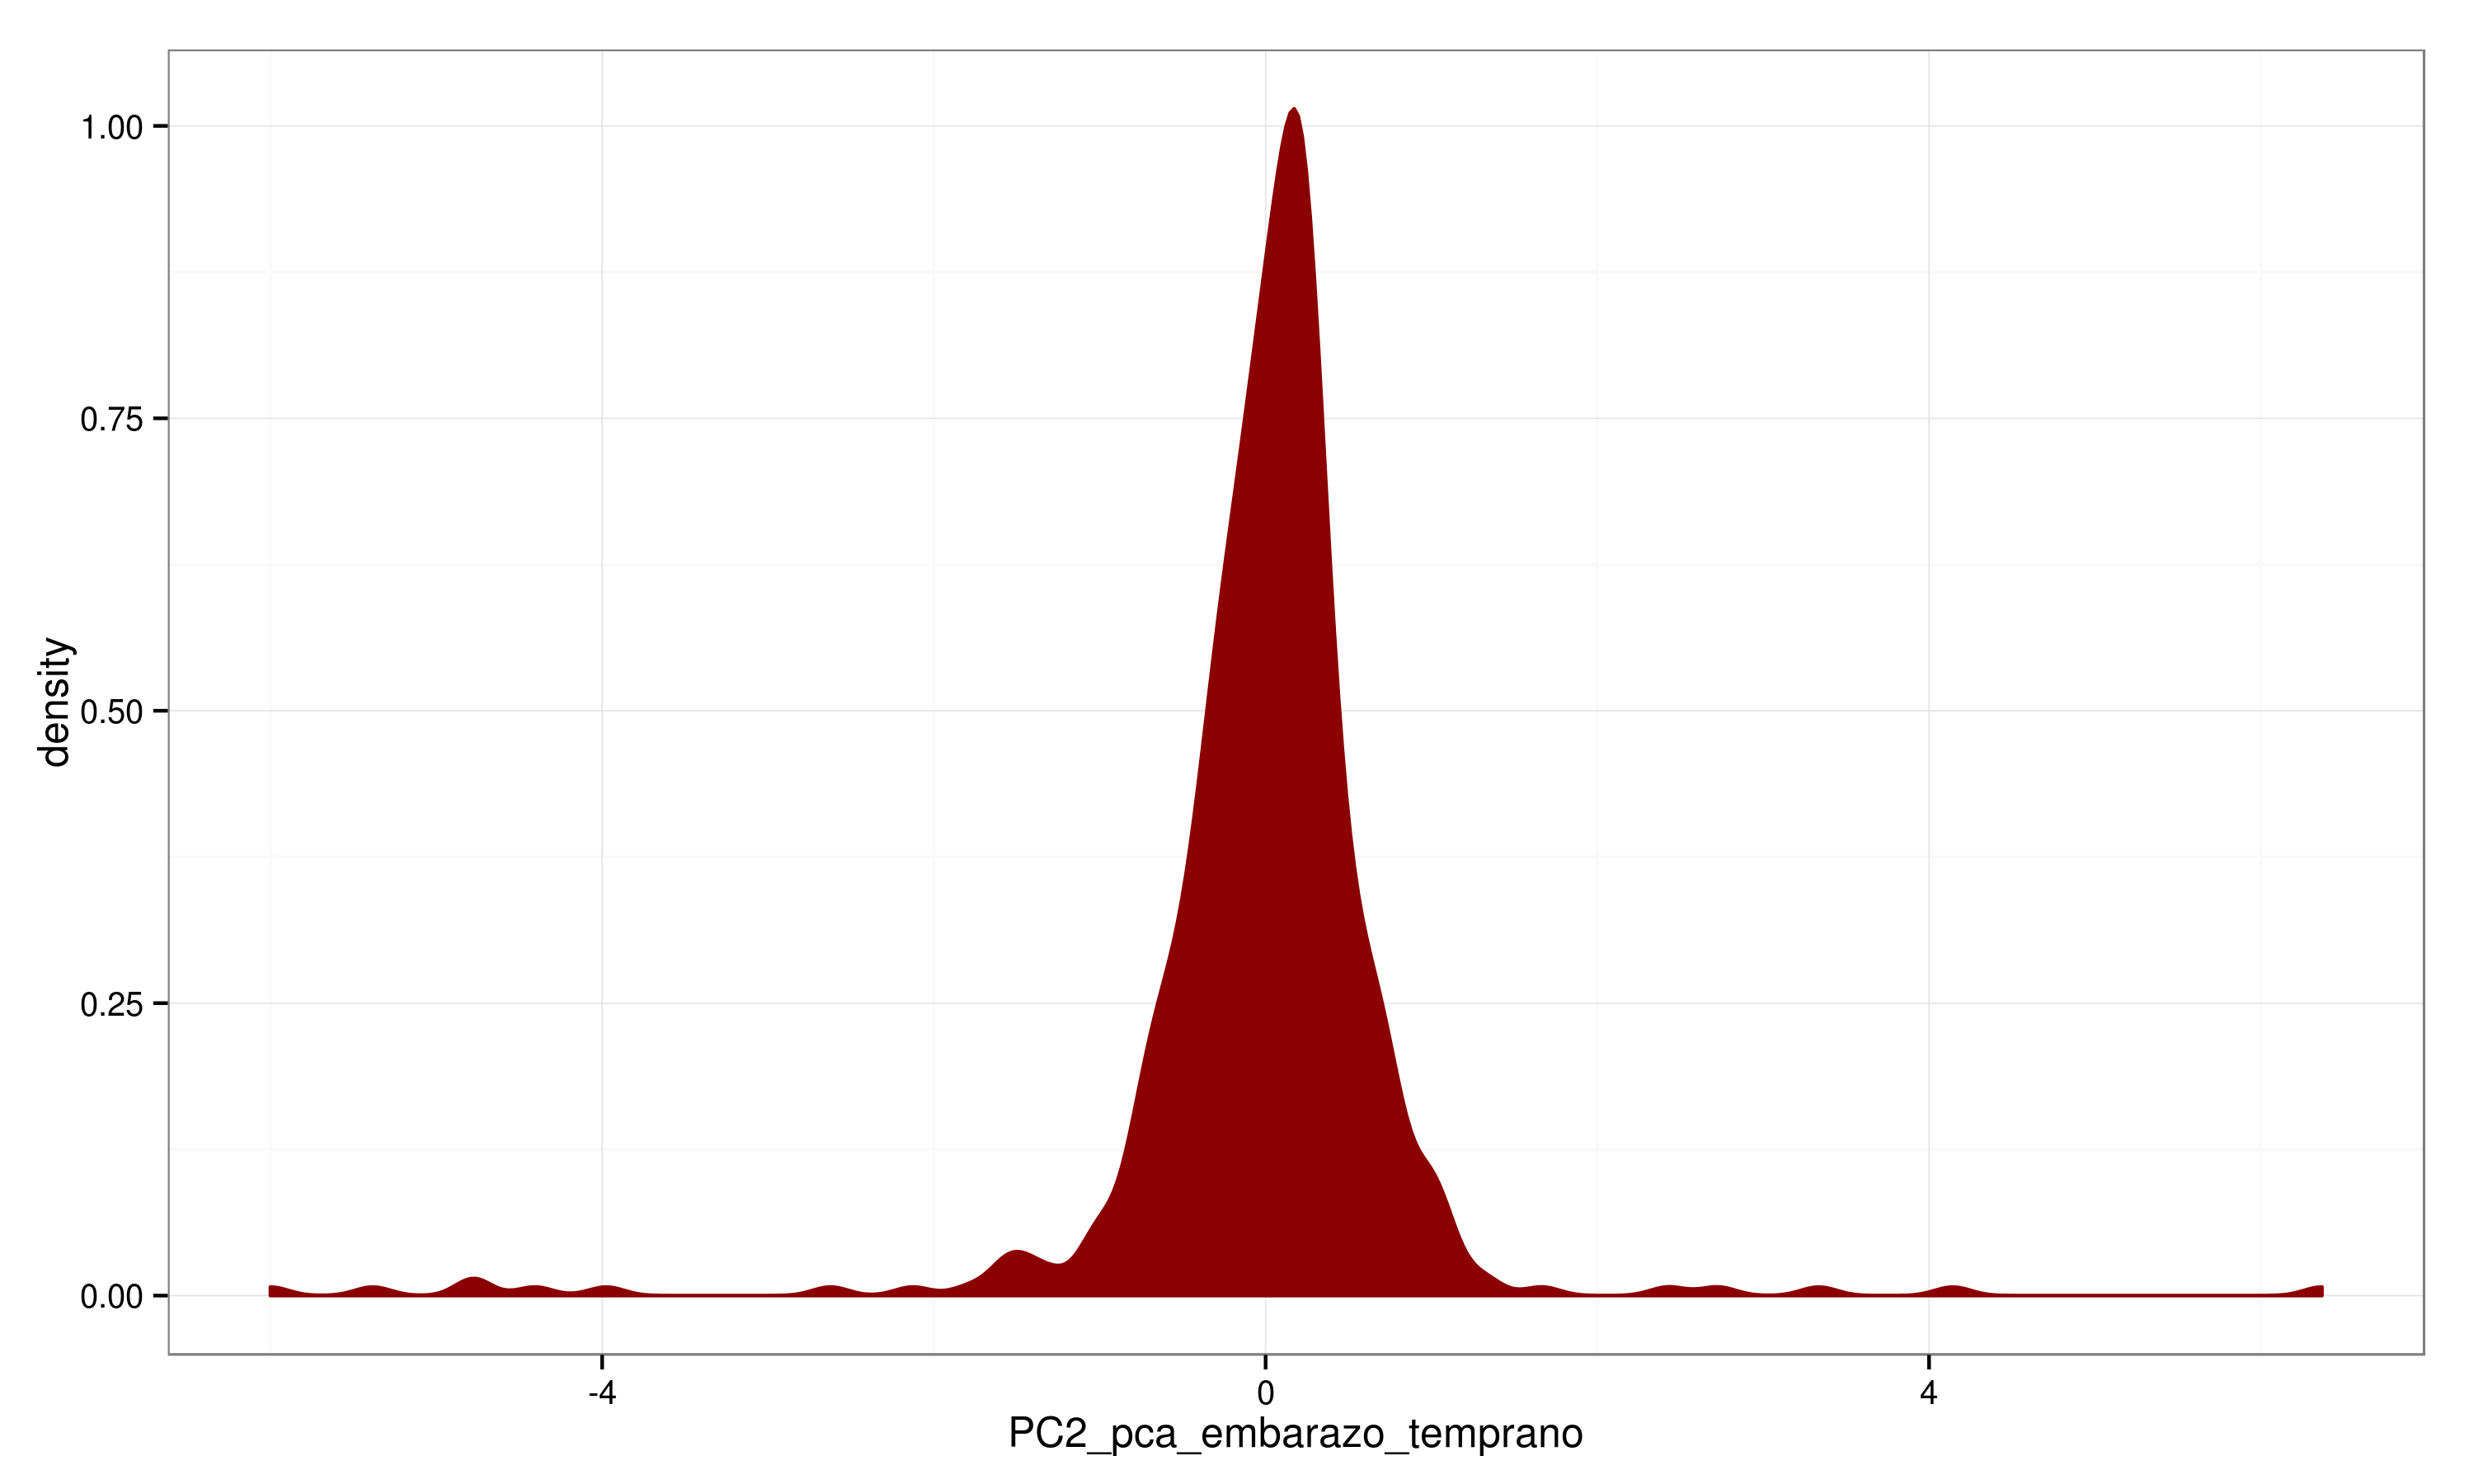
\includegraphics{img/x_density23.png}

\end{frame}

\begin{frame}{Factores de riesgo}

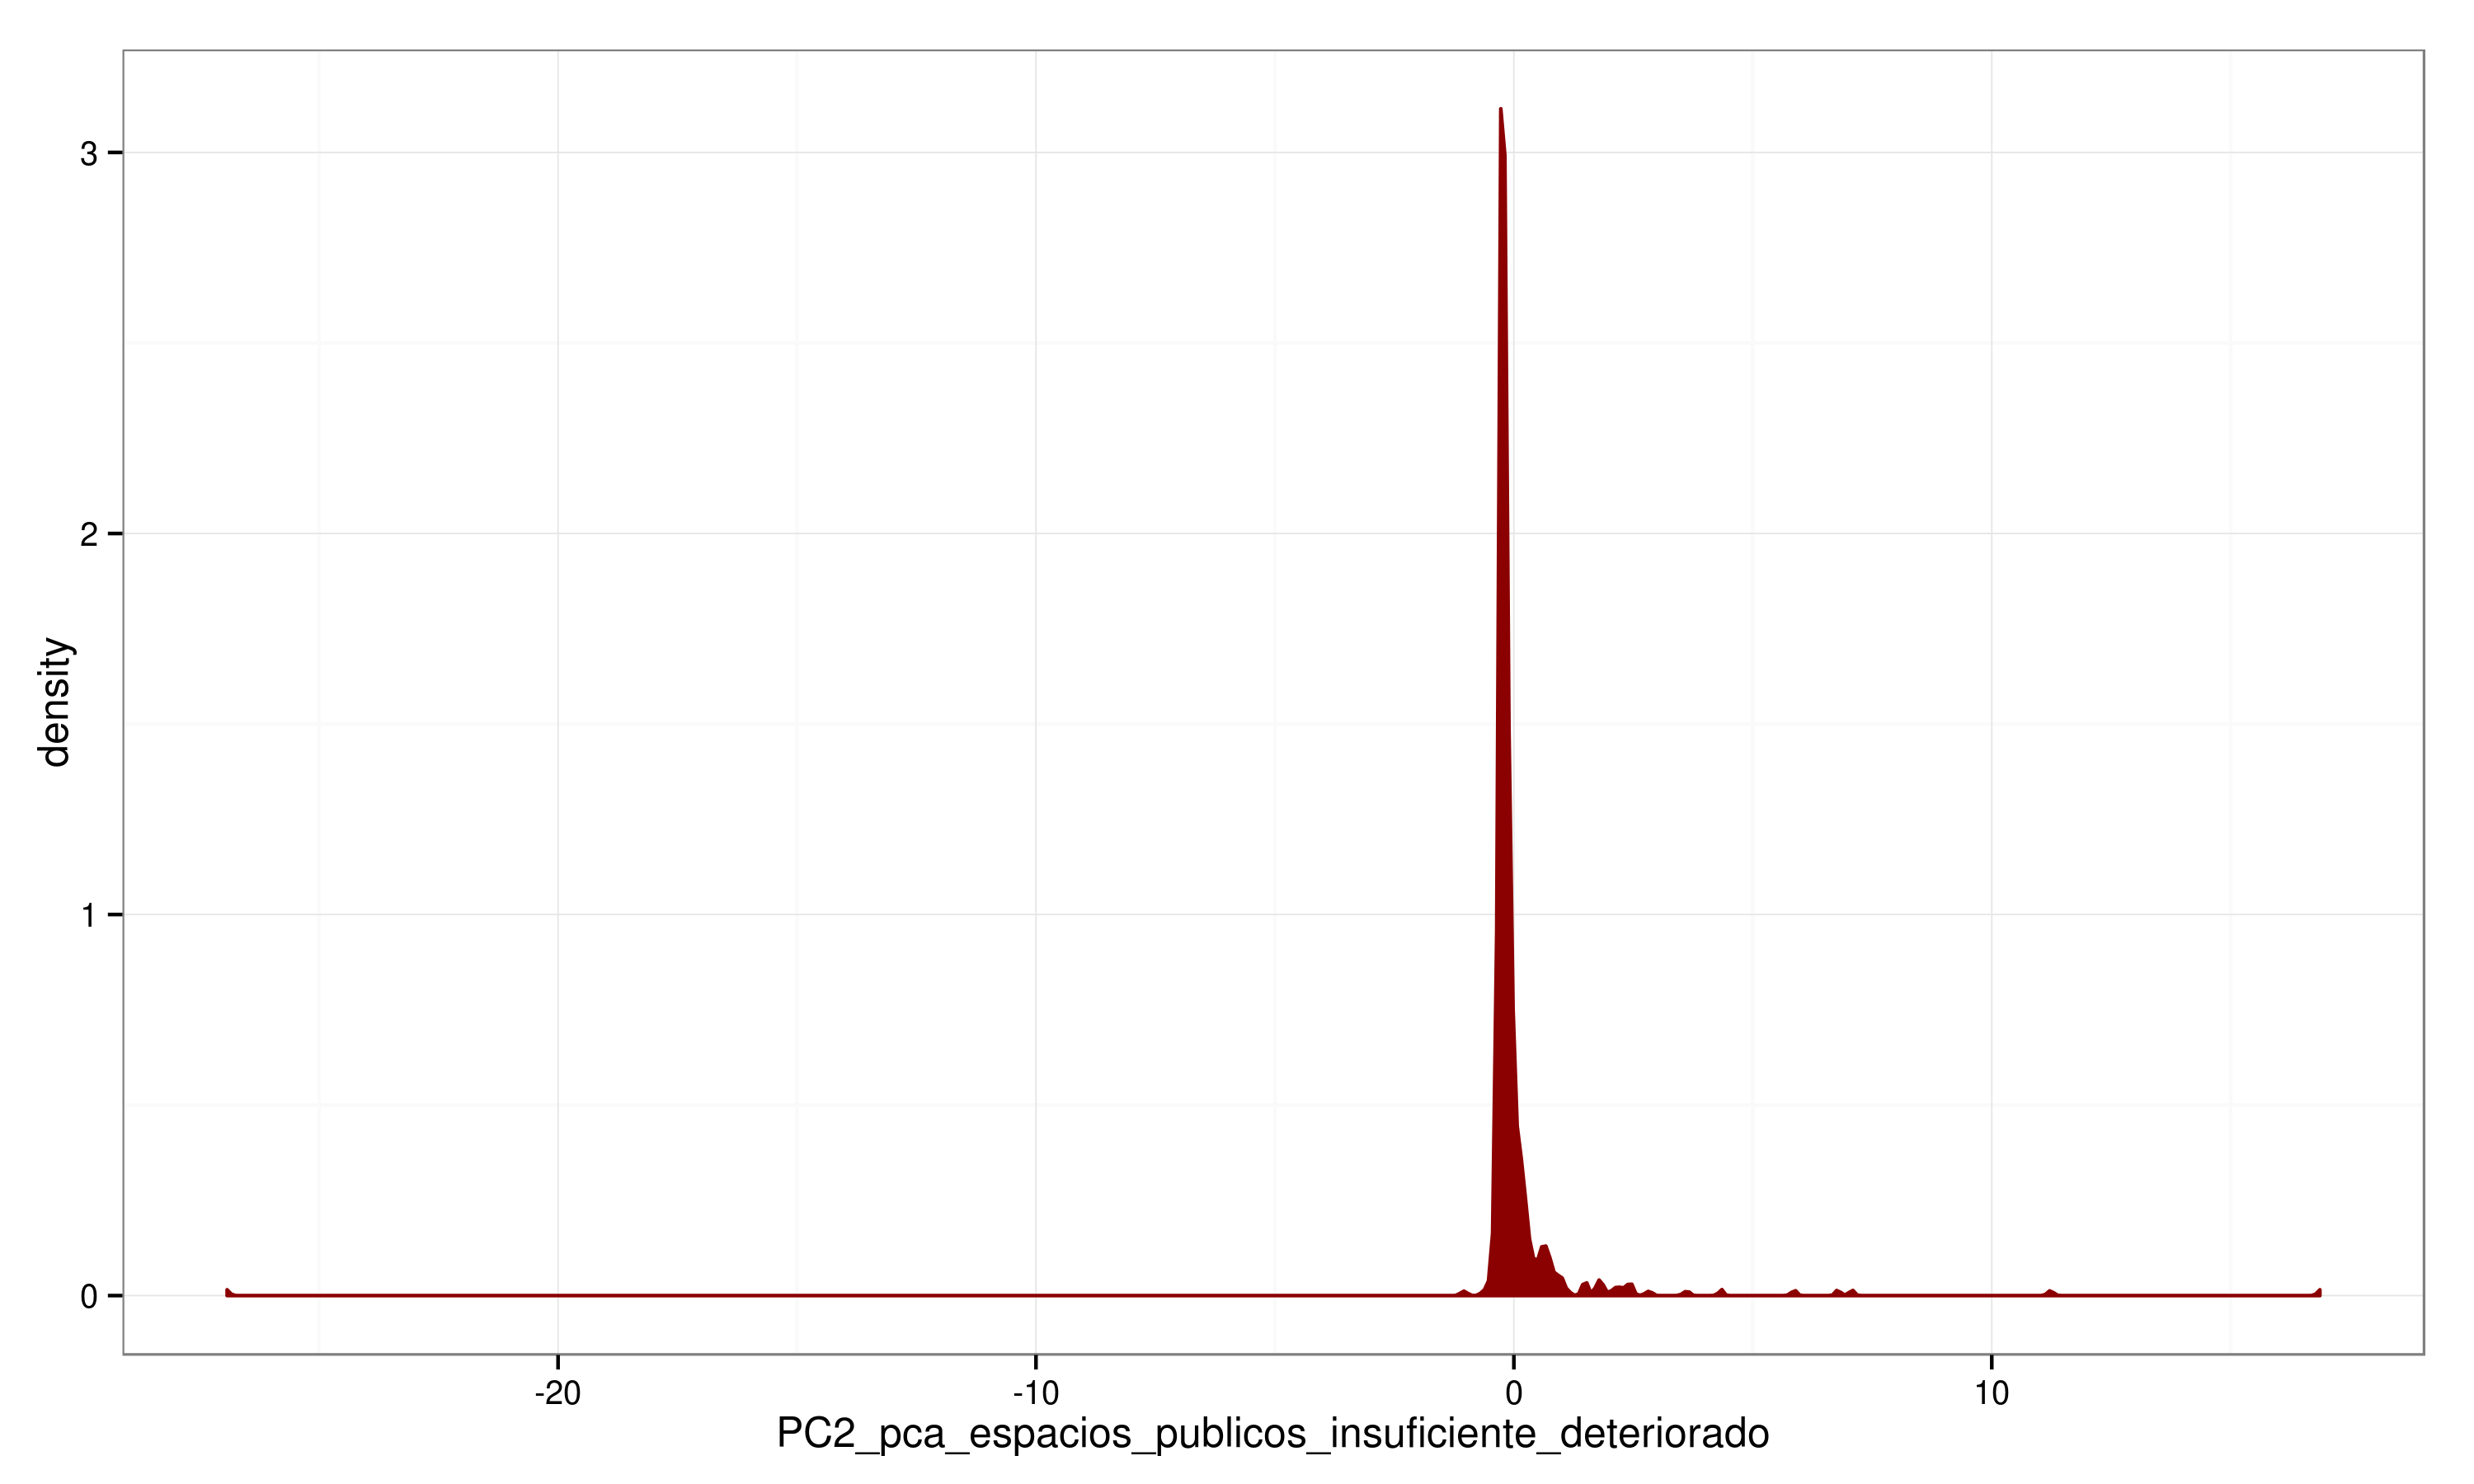
\includegraphics{img/x_density24.png}

\end{frame}

\begin{frame}{Factores de riesgo}

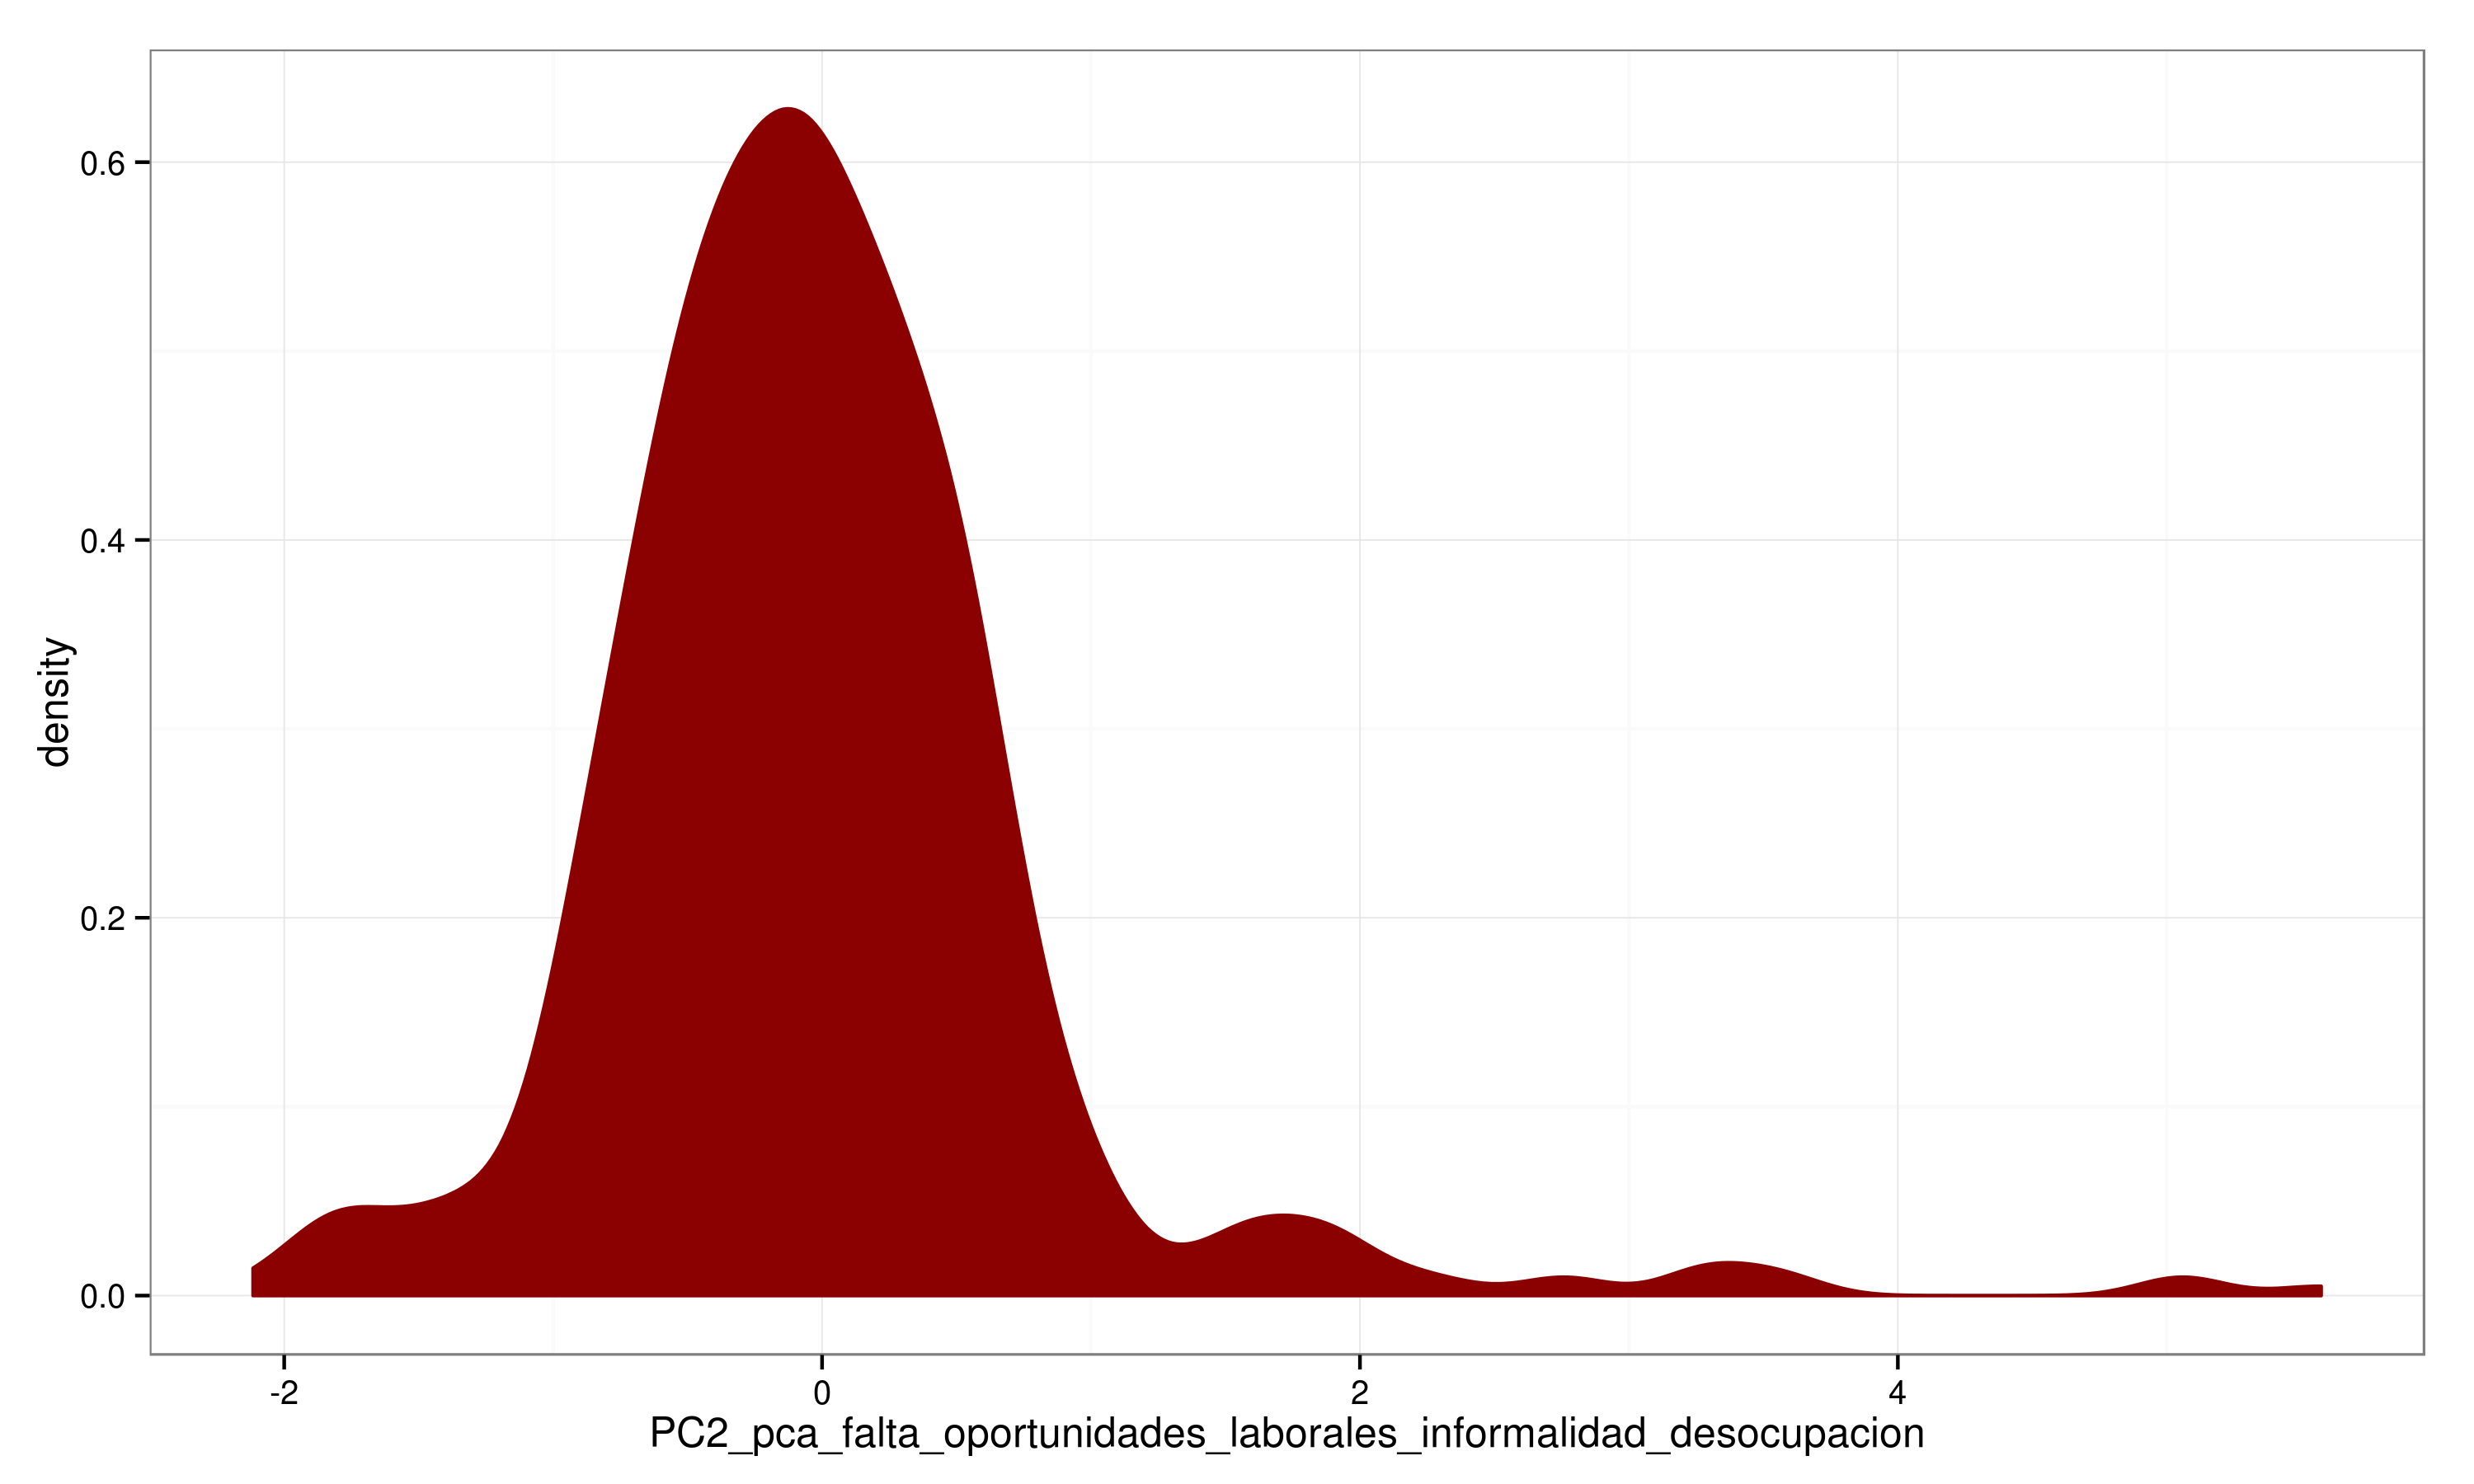
\includegraphics{img/x_density25.png}

\end{frame}

\begin{frame}{Factores de riesgo}

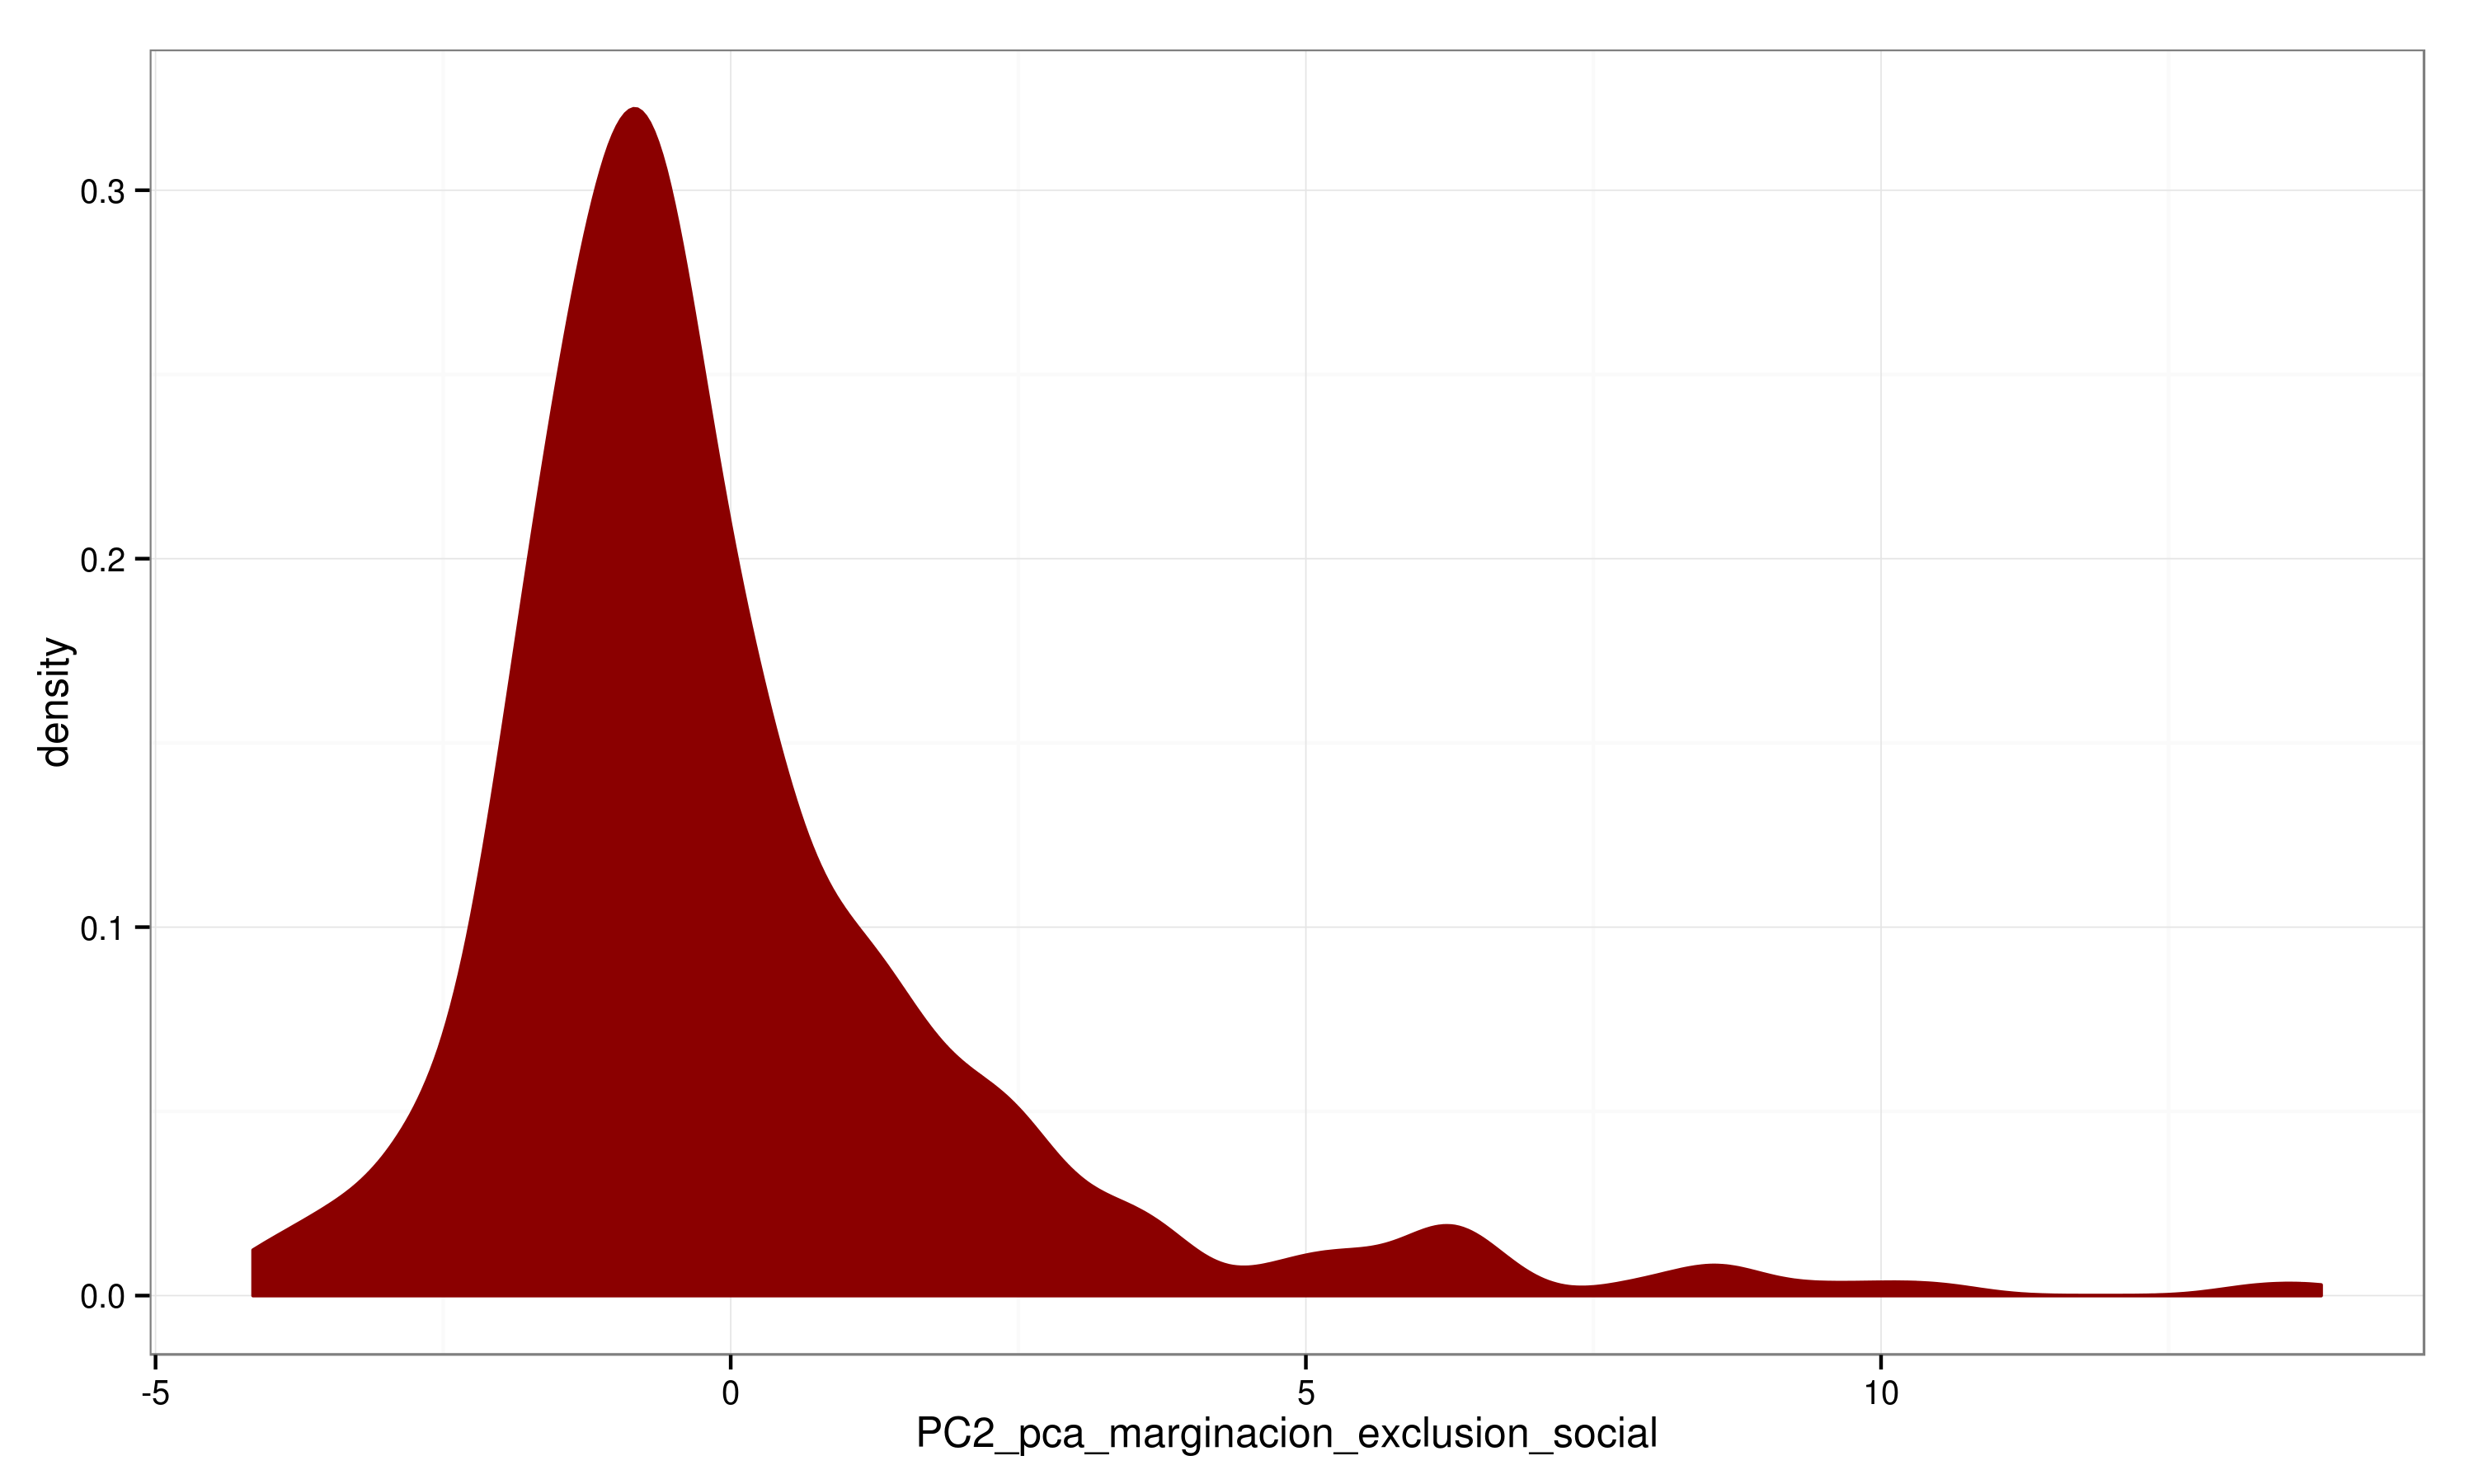
\includegraphics{img/x_density26.png}

\end{frame}

\begin{frame}{Modelo}

Siguiendo las recomendaciones del Dr.~Vilalta se decidió utilizar de
variables dependiente los delitos sumatoria de todos los delitos
ajustada por 100mil habitantes explicadas por los PCA 1 y 2 de los
factores de riesgo

\begin{block}{Modelo 1}

Delitos = factores de riesgo glm familia gaussiana

\end{block}

\begin{block}{Modelo 2}

log 1+Delitos = factores de riesgo glm familia gaussiana

\end{block}

\end{frame}

\begin{frame}{Modelos}

\begin{block}{Modelo 3}

Delitos = factores de riesgo glm familia poisson

\end{block}

\begin{block}{Modelo 4}

log 1+Delitos = factores de riesgo glm familia poisson

\end{block}

\begin{block}{Modelo 5}

Delitos = factores de riesgo glm familia quasi-poisson

\end{block}

\begin{block}{Modelo 6}

log 1+Delitos = factores de riesgo glm familia quasi- poisson

\end{block}

\end{frame}

\begin{frame}{Modelo Gaussiano, tasa de delito por cien mil habitantes}

\begin{table}[ht]
\centering
{\small
\begin{tabular}{rrrr}
  \hline
Estimate & Std. Error & t value & Pr($>$$|$t$|$) \\ 
  \hline
978.2956 & 29.0698 & 33.65 & 0.0000 \\ 
  99.0401 & 72.9292 & 1.36 & 0.1751 \\ 
  48.6531 & 33.2996 & 1.46 & 0.1447 \\ 
  40.5287 & 80.8543 & 0.50 & 0.6164 \\ 
  -13.5341 & 5.6351 & -2.40 & 0.0167 \\ 
  27.0878 & 25.6840 & 1.05 & 0.2921 \\ 
  -72.6210 & 65.6060 & -1.11 & 0.2689 \\ 
  -212.7272 & 80.1829 & -2.65 & 0.0082 \\ 
  -13.7080 & 20.7738 & -0.66 & 0.5097 \\ 
  -72.0285 & 105.6864 & -0.68 & 0.4959 \\ 
  72.9273 & 67.2275 & 1.08 & 0.2786 \\ 
  -20.8337 & 29.7304 & -0.70 & 0.4838 \\ 
  34.7370 & 10.2774 & 3.38 & 0.0008 \\ 
  -46.9624 & 35.7216 & -1.31 & 0.1893 \\ 
  66.1338 & 52.7209 & 1.25 & 0.2103 \\ 
  -109.6174 & 108.3881 & -1.01 & 0.3124 \\ 
  -11.9548 & 41.9198 & -0.29 & 0.7756 \\ 
   \hline
\end{tabular}
}
\end{table}

\end{frame}

\begin{frame}{Modelo Gaussiano, logaritmo de tasa de delito por cien mil
habitantes}

\begin{table}[ht]
\centering
{\small
\begin{tabular}{rrrr}
  \hline
Estimate & Std. Error & t value & Pr($>$$|$t$|$) \\ 
  \hline
6.2951 & 0.0783 & 80.44 & 0.0000 \\ 
  0.1265 & 0.1963 & 0.64 & 0.5196 \\ 
  0.0692 & 0.0896 & 0.77 & 0.4408 \\ 
  0.2155 & 0.2177 & 0.99 & 0.3227 \\ 
  -0.0589 & 0.0152 & -3.88 & 0.0001 \\ 
  0.0744 & 0.0691 & 1.08 & 0.2828 \\ 
  -0.1968 & 0.1766 & -1.11 & 0.2657 \\ 
  -0.5058 & 0.2159 & -2.34 & 0.0195 \\ 
  0.0827 & 0.0559 & 1.48 & 0.1398 \\ 
  -0.2230 & 0.2845 & -0.78 & 0.4335 \\ 
  0.1117 & 0.1810 & 0.62 & 0.5374 \\ 
  -0.0854 & 0.0800 & -1.07 & 0.2867 \\ 
  0.0700 & 0.0277 & 2.53 & 0.0117 \\ 
  -0.1722 & 0.0962 & -1.79 & 0.0741 \\ 
  0.1700 & 0.1419 & 1.20 & 0.2316 \\ 
  0.2443 & 0.2918 & 0.84 & 0.4028 \\ 
  -0.1825 & 0.1128 & -1.62 & 0.1065 \\ 
   \hline
\end{tabular}
}
\end{table}

\end{frame}

\begin{frame}{Modelo Poisson, tasa de delito por cien mil habitantes}

\begin{table}[ht]
\centering
{\small
\begin{tabular}{rrrr}
  \hline
Estimate & Std. Error & z value & Pr($>$$|$z$|$) \\ 
  \hline
6.8209 & 0.0016 & 4393.76 & 0.0000 \\ 
  0.1137 & 0.0039 & 29.39 & 0.0000 \\ 
  0.0811 & 0.0020 & 40.44 & 0.0000 \\ 
  0.0693 & 0.0037 & 18.62 & 0.0000 \\ 
  -0.0165 & 0.0003 & -53.74 & 0.0000 \\ 
  0.0305 & 0.0013 & 23.02 & 0.0000 \\ 
  -0.0733 & 0.0033 & -22.54 & 0.0000 \\ 
  -0.2166 & 0.0042 & -50.97 & 0.0000 \\ 
  -0.0365 & 0.0013 & -28.62 & 0.0000 \\ 
  -0.0724 & 0.0057 & -12.79 & 0.0000 \\ 
  0.0610 & 0.0032 & 19.15 & 0.0000 \\ 
  -0.0290 & 0.0016 & -17.97 & 0.0000 \\ 
  0.0491 & 0.0006 & 83.04 & 0.0000 \\ 
  -0.0483 & 0.0018 & -27.30 & 0.0000 \\ 
  0.0844 & 0.0027 & 31.40 & 0.0000 \\ 
  -0.0479 & 0.0056 & -8.57 & 0.0000 \\ 
  0.0068 & 0.0023 & 2.94 & 0.0033 \\ 
   \hline
\end{tabular}
}
\end{table}

\end{frame}

\begin{frame}{Modelo Poisson, logaritmo de tasa de delito por cien mil
habitantes}

\begin{table}[ht]
\centering
{\small
\begin{tabular}{rrrr}
  \hline
Estimate & Std. Error & z value & Pr($>$$|$z$|$) \\ 
  \hline
1.8365 & 0.0181 & 101.22 & 0.0000 \\ 
  0.0210 & 0.0450 & 0.47 & 0.6405 \\ 
  0.0106 & 0.0205 & 0.52 & 0.6040 \\ 
  0.0327 & 0.0487 & 0.67 & 0.5019 \\ 
  -0.0098 & 0.0036 & -2.71 & 0.0067 \\ 
  0.0133 & 0.0168 & 0.79 & 0.4292 \\ 
  -0.0299 & 0.0399 & -0.75 & 0.4542 \\ 
  -0.0768 & 0.0483 & -1.59 & 0.1119 \\ 
  0.0128 & 0.0128 & 1.00 & 0.3183 \\ 
  -0.0350 & 0.0646 & -0.54 & 0.5878 \\ 
  0.0166 & 0.0410 & 0.40 & 0.6855 \\ 
  -0.0129 & 0.0180 & -0.72 & 0.4743 \\ 
  0.0119 & 0.0065 & 1.82 & 0.0689 \\ 
  -0.0283 & 0.0223 & -1.27 & 0.2057 \\ 
  0.0255 & 0.0322 & 0.79 & 0.4286 \\ 
  0.0362 & 0.0658 & 0.55 & 0.5816 \\ 
  -0.0276 & 0.0251 & -1.10 & 0.2712 \\ 
   \hline
\end{tabular}
}
\end{table}

\end{frame}

\begin{frame}{Modelo Quasipoisson, tasa de delito por cien mil
habitantes}

\begin{table}[ht]
\centering
{\small
\begin{tabular}{rrrr}
  \hline
Estimate & Std. Error & t value & Pr($>$$|$t$|$) \\ 
  \hline
6.8209 & 0.0306 & 223.14 & 0.0000 \\ 
  0.1137 & 0.0762 & 1.49 & 0.1362 \\ 
  0.0811 & 0.0395 & 2.05 & 0.0406 \\ 
  0.0693 & 0.0733 & 0.95 & 0.3449 \\ 
  -0.0165 & 0.0060 & -2.73 & 0.0066 \\ 
  0.0305 & 0.0261 & 1.17 & 0.2429 \\ 
  -0.0733 & 0.0640 & -1.14 & 0.2530 \\ 
  -0.2166 & 0.0837 & -2.59 & 0.0099 \\ 
  -0.0365 & 0.0251 & -1.45 & 0.1468 \\ 
  -0.0724 & 0.1115 & -0.65 & 0.5163 \\ 
  0.0610 & 0.0628 & 0.97 & 0.3313 \\ 
  -0.0290 & 0.0318 & -0.91 & 0.3620 \\ 
  0.0491 & 0.0116 & 4.22 & 0.0000 \\ 
  -0.0483 & 0.0348 & -1.39 & 0.1662 \\ 
  0.0844 & 0.0529 & 1.59 & 0.1115 \\ 
  -0.0479 & 0.1101 & -0.44 & 0.6637 \\ 
  0.0068 & 0.0455 & 0.15 & 0.8814 \\ 
   \hline
\end{tabular}
}
\end{table}

\end{frame}

\begin{frame}{Modelo Quasipoisson, logaritmo de tasa de delito por cien
mil habitantes}

\begin{table}[ht]
\centering
{\small
\begin{tabular}{rrrr}
  \hline
Estimate & Std. Error & t value & Pr($>$$|$t$|$) \\ 
  \hline
1.8365 & 0.0127 & 144.52 & 0.0000 \\ 
  0.0210 & 0.0315 & 0.67 & 0.5052 \\ 
  0.0106 & 0.0143 & 0.74 & 0.4593 \\ 
  0.0327 & 0.0341 & 0.96 & 0.3382 \\ 
  -0.0098 & 0.0025 & -3.87 & 0.0001 \\ 
  0.0133 & 0.0118 & 1.13 & 0.2596 \\ 
  -0.0299 & 0.0279 & -1.07 & 0.2858 \\ 
  -0.0768 & 0.0339 & -2.27 & 0.0237 \\ 
  0.0128 & 0.0090 & 1.42 & 0.1549 \\ 
  -0.0350 & 0.0452 & -0.77 & 0.4394 \\ 
  0.0166 & 0.0287 & 0.58 & 0.5634 \\ 
  -0.0129 & 0.0126 & -1.02 & 0.3075 \\ 
  0.0119 & 0.0046 & 2.60 & 0.0097 \\ 
  -0.0283 & 0.0157 & -1.81 & 0.0715 \\ 
  0.0255 & 0.0226 & 1.13 & 0.2589 \\ 
  0.0362 & 0.0461 & 0.79 & 0.4319 \\ 
  -0.0276 & 0.0176 & -1.57 & 0.1168 \\ 
   \hline
\end{tabular}
}
\end{table}

\end{frame}

\begin{frame}{Comparación de Modelos}

\[ \begin{tabular}{rlrrr}
  \hline
 & .id & AIC & Dev & BIC \\ 
  \hline
1 & mod & 7695.79 & 193136137.25 & 7771.18 \\ 
  2 & mod\_log & 1932.16 & 1399.60 & 2007.55 \\ 
  3 & mod\_poiss & Inf & 196419.01 & Inf \\ 
  4 & mod\_q\_poiss &  & 196419.01 &  \\ 
  5 & mod\_poiss\_log & Inf & 405.68 & Inf \\ 
  6 & mod\_q\_poiss\_log &  & 405.68 &  \\ 
   \hline
\end{tabular} \]

\end{frame}

\begin{frame}{Selección de Variables}

se quitaron as siguientes variables PC1\_pca\_desercion\_escolar -
PC2\_pca\_espacios\_publicos\_insuficiente\_deteriorado -
PC2\_pca\_consumo\_abuso\_drogas\_ilegales -
PC1\_pca\_espacios\_publicos\_insuficiente\_deteriorado -
PC1\_pca\_embarazo\_temprano -
PC1\_pca\_consumo\_abuso\_drogas\_ilegales -
PC2\_pca\_embarazo\_temprano,

\end{frame}

\begin{frame}{Conclusiones}

El modelo poisson con la variable sin transformar obtiene peor devianza
que el modelo gaussiano con la variable y transformada. Sin embargo, los
supuestos del modelo se sostienen mejor en el modelo Poisson. Tanto el
modelo poisson como el quasipoisson son iguales en devianza y los
supuestos se cumplen de manera aceptable.

\end{frame}

\begin{frame}{Recomendaciones}

-El análisis muestra que existen diferentes clasificaciones por
municipio donde se presentan los factores de riesgo y además se agrupan
espacialmente. Por lo tanto la intervención para atacar estos factores
debe ser diferenciada por municipio y por tipo de factor de riesgo. Por
ejemplo, aquellos municipios donde el deterioro de los espacios públicos
aparece como un factor de riesgo, deberán priorizar intervenciones para
la mejora de espacios públicos.

\end{frame}

\begin{frame}{Gasto}

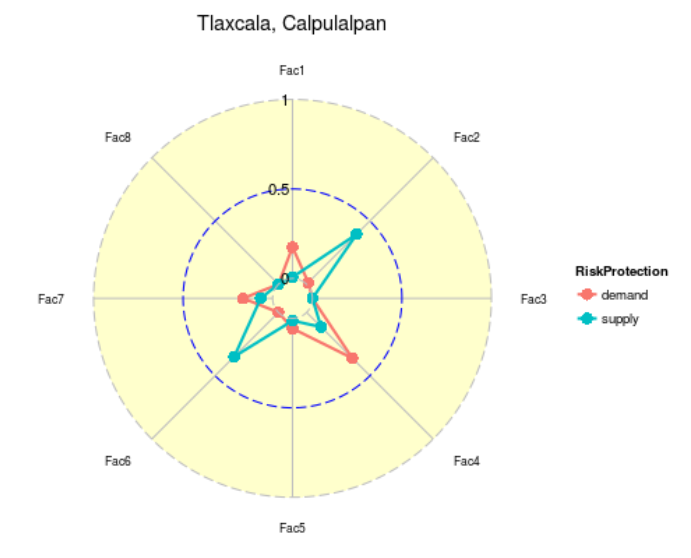
\includegraphics{img/gasto.png}

\end{frame}

\end{document}
